%\title{3cauVMF}
\documentclass[12pt,twoside]{article} 
\usepackage[a4paper,tmargin=1.5cm, bmargin=2cm, lmargin=1.5cm, rmargin=1.5cm]{geometry}
\usepackage{graphicx}
\usepackage{amsmath,amssymb,latexsym,amsfonts, bbm,mathtools, enumitem,esvect,commath,pifont}
\usepackage{fourier}
\usepackage[utf8]{vietnam}
\usepackage{tabvar}
\usepackage{tikz,pgf,tkz-tab}
\usepackage{multicol}
\usepackage{pdfpages}
\usepackage{fancyhdr}
\pagestyle{fancy}
\lhead[]{}\chead[]{}\rhead[]{}
\lfoot[\sl Trang \thepage]{\it http://diendantoanhoc.net}\cfoot[]{}\rfoot[\it http://diendantoanhoc.net]{\sl Trang \thepage}
\renewcommand{\headrulewidth}{0pt}
\renewcommand{\footrulewidth}{1pt}  
\setlength{\parindent}{0pt}

%%---code dùng để đóng khung 
\usepackage[framemethod=tikz]{mdframed}
\usetikzlibrary{shadows}
\newcounter{bai}[section]
\newenvironment{Fancybox}[1][\textwidth]
{\stepcounter{bai}%
  \mdfsetup{
      singleextra={%
      \node[draw=gray!100,anchor=east,rectangle, thick,font=\color{black},
     top color=green!40, bottom color=blue!5,
     rounded corners=3pt,minimum height=5mm, minimum width = 15mm] at ([xshift=60pt]O|-P){\strut \bf Bài~\thebai}; 
		},%
    apptotikzsetting={\tikzset{mdfbackground/.append style={shade, left color=blue!25, right color=white}}},
    frametitleaboveskip=\dimexpr-\ht\strutbox\relax,
   % skipabove=\topskip,
    skipbelow=\topskip,
    rightline=true,
    innertopmargin=18pt,innerleftmargin=10pt,innerrightmargin=10pt,
    roundcorner=5pt,
    linecolor=gray,%
    innerlinewidth=1pt,
    topline=true,
    shadow=true,
    shadowsize=5pt,
    shadowcolor=gray!100
  }
  \begin{mdframed}[userdefinedwidth=#1]\relax%
}
{\end{mdframed}}

\newcounter{vdu}[section]
\newenvironment{Fancyboxv}[1][\textwidth]
{\stepcounter{vdu}%
  \mdfsetup{
      singleextra={%
      \node[draw=gray!100,anchor=east,rectangle, thick,font=\color{black},
     top color=green!40, bottom color=blue!5,
     rounded corners=3pt,minimum height=5mm, minimum width = 15mm] at ([xshift=60pt]O|-P){\strut \bf Ví dụ~\thevdu}; 
		},%
    apptotikzsetting={\tikzset{mdfbackground/.append style={shade, left color=blue!25, right color=white}}},
    frametitleaboveskip=\dimexpr-\ht\strutbox\relax,
   % skipabove=\topskip,
    skipbelow=\topskip,
    rightline=true,
    innertopmargin=18pt,innerleftmargin=10pt,innerrightmargin=10pt,
    roundcorner=5pt,
    linecolor=gray,%
    innerlinewidth=1pt,
    topline=true,
    shadow=true,
    shadowsize=5pt,
    shadowcolor=gray!100
  }
  \begin{mdframed}[userdefinedwidth=#1]\relax%
}
{\end{mdframed}}

% - các newcommand để gõ tắt kí hiệu

\newcounter{debai}[section]
\def\thedebai{\arabic{debai}}
\newcommand{\debai}[1]{\refstepcounter{debai}{\strut \bf Bài ~\thedebai. } #1 \bigskip}
\newcommand{\deda}[1]{\begin{Fancybox}#1 \end{Fancybox}}
\newcommand{\vidu}[1]{\begin{Fancyboxv}#1 \end{Fancyboxv}}
\newcommand{\lgi}{\begin{center} \bf Lời giải \end{center} } 
\newcommand{\hda}{\begin{center} \bf Hướng dẫn \end{center} } 
\newcommand{\nxe}{\textbf{Nhận xét:} } 
\newcommand{\cl}[1]{\centerline{#1}}
\newcommand{\hay}[1]{\left[\begin{array}{ll}#1\end{array}\right.}
\newcommand{\va}[1]{\left\{\begin{array}{ll}#1\end{array}\right.}
\newcommand{\vt}[1]{\overrightarrow{#1}}
\newcommand{\bd}{Trong mặt phẳng với hệ tọa độ $Oxy$,\,}
\newcommand{\hpt}[1]{\left\{ \begin{array}{l} #1 \end{array}\right.}
\newcommand{\goc}[1]{\widehat{#1}}
\newcommand{\hoac}[1]{\left[ \begin{array}{l} #1 \end{array}\right.}

\title{TUYỂN TẬP BỘ BA CÂU PHÂN LOẠI\\ TRONG ĐỀ THI THỬ \\ TRUNG HỌC PHỔ THÔNG QUỐC GIA 2015}
\author{VMF}
\date{Ngày 6 tháng 10 năm 2015}

\everymath{\displaystyle}
\begin{document}

\includepdf[pages={1},scale=1.0]{bia.pdf}
\newpage
\thispagestyle{empty}
\text{ }

\newpage
\maketitle
\thispagestyle{empty}
{\Large LỜI NÓI ĐẦU}

\hspace{10mm} Xuất phát từ thực tế kì thi THPT Quốc gia 2015, với các bạn sử dụng kết quả môn Toán để xét tuyển đại học, thì sự cạnh tranh chủ yếu diễn ra ở bộ ba câu phân loại. Bộ ba câu này thường rơi vào các chủ đề Phương trình - Bất phương trình - Hệ phương trình, Hình học tọa độ phẳng, Bất đẳng thức - Tìm GTLN NN.
\vspace{5mm}
 
\hspace{10mm} Nhằm mục đích cung cấp thêm cho các bạn chuẩn bị tham gia kì thi THPT Quốc gia 2016 một tài liệu tham khảo hữu ích, các thành viên của diễn đàn toán học VMF đã cùng nhau biên soạn tài liệu này. Tài liệu tổng hợp lại các câu hỏi thuộc 3 chủ đề nói trên trong các đề thi thử năm học 2014 - 2015. Phần hướng dẫn, đáp số chúng tôi chủ yếu dựa trên đáp án của đơn vị ra đề, tuy nhiên trong một số bài toán chúng tôi có đưa ra cách tiếp cận khác, hoặc chỉ hướng dẫn sơ lược có đáp số nhằm giúp bạn đọc chủ động hơn trong quá trình đọc tài liệu. Chúng tôi nhấn mạnh rằng, cách làm trong tài liệu này chưa hẳn là tốt nhất, bạn đọc cũng không nên quá coi trọng các lời giải mang đậm chất kĩ thuật, khó định hướng tự nhiên.
\vspace{5mm}
 

\hspace{10mm} Nhóm biên soạn tài liệu này gồm có\\
•Bạn Trần Tuấn Anh, Nguyễn Nguyên Trang - Sinh viên khoa Toán ĐHSP TP.HCM (Katyusha);\\
•Bạn Trương Việt Hoàng - THPT Nguyễn Du, Thái Bình (Viet Hoang 99);\\
•Thầy Châu Ngọc Hùng - Ninh Thuận (hungchng);\\
•Thầy Nguyễn Công Định - Cà Mau (CD13);\\
•Thầy Hoàng Ngọc Thế - Hà Nội (E.Galois);\\
•Thầy Lê Minh An - Nam Định (leminhansp).
\vspace{5mm}

\hspace{10mm} Mặc dù chúng tôi đã cùng nhau biên soạn tài liệu này với tất cả sự tận tâm, tinh thần vì cộng đồng vô tư. Nhưng sự tỉ mỉ và cố gắng của chúng tôi chắc chắn chưa thể kiểm soát được hết các sai sót. Vì vậy sự nhiệt tâm từ phía bạn đọc cũng sẽ giúp tài liệu hoàn thiện hơn. Mọi trao đổi hãy chia sẻ với chúng tôi tại diễn đàn toán học VMF.
http://diendantoanhoc.net/forum/
\vspace{5mm}

\hspace{10mm} Sau cùng, chúng tôi hi vọng cộng đồng chia sẻ trực tuyến sẽ dành cho chúng tôi sự tôn trọng tối thiểu bằng cách ghi rõ nguồn tài liệu khi chia sẻ. Không dùng tài liệu này để trục lợi cá nhân. Chúng tôi xin cảm ơn!
\vspace{5mm}

\hspace{12cm} Nhóm biên tập

%\newpage\tableofcontents

%\newpage\part*{I. PHƯƠNG PHÁP TỌA ĐỘ TRONG MẶT PHẲNG}
\addcontentsline{toc}{part}{I. PHƯƠNG PHÁP TỌA ĐỘ TRONG MẶT PHẲNG}
\section{Lý thuyết chung}
\subsection{Hệ tọa độ}
Trong mặt phẳng với hệ tọa độ $Oxy$ cho các điểm: $A\left(x_A;y_A\right), B\left(x_B;y_B\right), C\left(x_C;y_C\right)$.
\begin{itemize}
\item Tọa độ vectơ: $\overrightarrow{AB} = \left(x_B-x_A;y_B-y_A\right)$
\item Tọa độ trung điểm $J$ của đoạn thẳng $AB$, trọng tâm $G$ của tam giác $ABC$ lần lượt là: 
$$J\left( \dfrac{x_A+x_B}{2}; \dfrac{y_A+y_B}{2}\right); \quad G\left( \dfrac{x_A+x_B+x_C}{3}; \dfrac{y_A+y_B+y_C}{3}\right)$$
\end{itemize}
\subsection{Phương trình đường thẳng}
\subsubsection{ Vectơ chỉ phương và vectơ pháp tuyến của đường thẳng:}
\begin{itemize}
\item Vectơ $\overrightarrow u (\overrightarrow u \neq \overrightarrow 0) $ là \textbf{vectơ chỉ phương} của đường thẳng $d$ nếu nó có giá song song hoặc trùng với đường thẳng $d$.
\item Vectơ $\overrightarrow n (\overrightarrow n \neq \overrightarrow 0) $ là \textbf{vectơ pháp tuyến} của đường thẳng $d$ nếu nó có giá vuông góc với đường thẳng $d$.
\item Đường thẳng $ax + by + c = 0$ có một vectơ pháp tuyến là $\overrightarrow n = (a; b)$.
\item Hai đường thẳng song song có cùng vectơ chỉ phương (vectơ pháp tuyến).
\item Hai đường thẳng vuông góc có vectơ pháp tuyến của đường thẳng này là vectơ chỉ phương của đường thẳng kia.
\item Nếu $\overrightarrow u, \overrightarrow n$ lần lượt là vectơ chỉ phương, vectơ pháp tuyến của đường thẳng $d$ thì $\overrightarrow u. \overrightarrow n = 0$. Do đó, nếu $\overrightarrow u = (a;b)$ thì $\overrightarrow n = (b; -a)$.
\item Một đường thẳng có vô số vectơ pháp tuyến, vô số vectơ chỉ phương. Nếu $\overrightarrow n$ là một vectơ pháp tuyến (vectơ chỉ phương) của đường thẳng $d$ thì $k\overrightarrow n (k \neq 0)$ cũng là một vectơ pháp tuyến, vectơ chỉ phương của $d$.
\end{itemize} 
\subsubsection{Phương trình đường thẳng}
\begin{itemize}
\item \textbf{Phương trình tổng quát} của đường thẳng: 
\begin{equation}
ax + by + c = 0\quad (a^2+b^2>0)
\end{equation}
Đường thẳng đi qua điểm $M(x_0;y_0)$ và nhận $\overrightarrow n = (a; b)$ là vectơ pháp tuyến có phương trình dạng:
\begin{equation}
a(x-x_0) + b(y-y_0) = 0
\end{equation}
Đặc biệt: đường thẳng đi qua $(a; 0), (0; b)$ có \textbf{phương trình theo đoạn chắn}:
\begin{equation}
\dfrac{x}{a}+\dfrac{y}{b}=1
\end{equation}
* Đường thẳng đi qua $M(x_0; y_0)$ và nhận vectơ $\overrightarrow n=(p;q)$ làm vectơ chỉ phương, có \textbf{phương trình tham số} là:
\begin{equation}
\left\{\begin{array}{l} x=x_0+pt\\y=y_0+qt \end{array}\right.
\end{equation}
Có \textbf{phương trình chính tắc} là:
\begin{equation}
\dfrac{x-x_0}{p}=\dfrac{y-y_0}{q} \quad (p,q \neq 0)
\end{equation}
\textbf{Đặc biệt}: đường thẳng đi qua 2 điểm phân biệt $A\left(x_A;y_A\right), B\left(x_B;y_B\right)$ có phương trình dạng:
\begin{equation}
\dfrac{{x - x_A }}{{x_B - x_A }} = \dfrac{{y - y_A }}{{y_B - y_A }}
\end{equation}
\item Đường thẳng đi qua $M(x_0;y_0)$ và có hệ số góc $k$ thì có \textbf{phương trình đường thẳng với hệ số góc} dạng:
\begin{equation}
y=k(x-x_0)+y_0
\end{equation}
\textbf{Chú ý:}
\begin{itemize}
\item Không phải đường thẳng nào cũng có hệ số góc. Các đường thẳng dạng $x=a$ không có hệ số góc. Do vậy, khi giải các bài toán dùng hệ số góc, ta phải xét cả trường hợp đặc biệt này.
\item Nếu $\overrightarrow n = (a; b)$ là vectơ pháp tuyến của đường thẳng thì hệ số góc của nó là $k = -\dfrac{a}{b}, b\neq 0.$
\end{itemize}
\end{itemize}
\subsubsection{Vị trí tương đối của 2 điểm và 1 đường thẳng}
Cho $A\left(x_A;y_A\right),B\left(x_B;y_B\right)$ và đường thẳng $\Delta: ax + by+ c = 0$. Khi đó:
\begin{itemize}
\item Nếu $\left(ax_A + by_A+ c \right)\left(ax_B + by_B+ c \right) <0$ thì $A,B$ ở về hai phía khác nhau đối với $\Delta$.
\item Nếu $\left(ax_A + by_A+ c \right)\left(ax_B + by_B+ c \right) >0$ thì $A,B$ ở cùng một phía đối với $\Delta$
\end{itemize}
\subsection{Góc và khoảng cách}
\begin{itemize}
\item Góc giữa hai vectơ $\vec{v}, \vec{w}$ được tính dựa theo công thức:
\begin{equation} \label{goc2vt}
\cos (\vec{u}, \vec{w}) = \dfrac{\vec{u}.\vec{w}}{\left | \vec{v} \right|.\left | \vec{w} \right| }
\end{equation}
\item Giả sử $\overrightarrow n_1,\overrightarrow n_2$ lần lượt là vectơ pháp tuyến của các đường thẳng $d_1$ và $d_2$. Khi đó:
\begin{equation} \label{goc2dt}
cos(d_1, d_2) = \dfrac{{\left| {\overrightarrow n _1 .\overrightarrow n _2 } \right|}}{{\left| {\overrightarrow n _1 } \right|.\left| {\overrightarrow n _2 } \right|}}
\end{equation}
\item Độ dài vectơ $\vec{u}=(a;b)$ là: 
\begin{equation}
\left|\vec{u}\right| = \sqrt{a^2+b^2}
\end{equation}
\item Khoảng cách giữa hai điểm $A(x_A;y_A),B(x_B;y_B)$ là:
\begin{equation}\label{ab}
AB = \sqrt{\left(x_B-x_A\right)^2+\left(y_B-y_A\right)^2}
\end{equation}
\item Diện tích tam giác $ABC$ là:
\begin{equation} \label{dttg}
S=\dfrac{1}{2}\sqrt{\left ( AB.AC \right )^2 - \left (\overrightarrow{AB}.\overrightarrow{AC}  \right )^2}
\end{equation}
\item Khoảng cách từ điểm $M(x_0; y_0)$ đến đường thẳng $d:ax+by+c=0$ được tính bằng công thức:
\begin{equation}\label{kc}
d_{(M; d)} = \dfrac{{\left| {ax_0 + by_0 + c} \right|}}{{\sqrt {a^2 + b^2 } }}
\end{equation}
\end{itemize}
\subsection{Phương trình đường tròn}
\begin{itemize}
\item Đường tròn tâm $I(a; b)$, bán kính $R$ có dạng:
\begin{equation}
(x-a)^2 + (y-b)^2 = R^2
\end{equation}
\item Phương trình:
\begin{equation} \label{dtrtq}
x^2 + y^2 + 2ax + 2by + c = 0, \quad (a^2 + b^2-c > 0)
\end{equation}
cũng là phương trình đường tròn với tâm $I(- a ;-b)$ và bán kính $R=\sqrt{a^2+b^2-c}$.
\item Phương trình tiếp tuyến của đường tròn tại điểm $M(x_0 ; y_0)$
\begin{equation}
(x_0-a)(x-x_0) + (y_0-b)(y-y_0) = 0
\end{equation}
\item Vị trí tương đối của đường thẳng $\Delta$ và đường tròn $\left(C\right)$ tâm $I$, bán kính $R$.
\begin{itemize}
\item Nếu $d_{(I;\Delta)} > R$ thì $\Delta$ và $\left(C\right)$ không cắt nhau.
\item Nếu $d_{(I;\Delta)} = R$ thì $\Delta$ và $\left(C\right)$ tiếp xúc tại $I'$ là hình chiếu của $I$ lên $d$.
\item Nếu $d_{(I;\Delta)} < R$ thì $\Delta$ và $\left(C\right)$ cắt nhau tại hai điểm $M,N$. Khi đó trung điểm $H$ của $MN$ là hình chiếu của $I$ lên $MN$ và 
\begin{equation}
MN= 2\sqrt{R^2-d^2_{(I,\Delta)}}
\end{equation}
\end{itemize}
\end{itemize} 
\subsection{Phương trình Elip}
\begin{itemize}
\item Elip là tập hợp các điểm $M$ di động thỏa mãn $MF_1+MF_2=2a$ với $F_1, F_2$ cố định, $F_1F_2=2c$, $a>c>0$ là các số cho trước. 
\item $F_1(-c;0)$,$F_2(c;0)$ được gọi là \textbf{tiêu điểm}, $F_1F_2=2c$ được gọi là \textbf{tiêu cự}. $MF_1,MF_2$ là các \textbf{bán kính qua tiêu}.
\item Các điểm $A_1(-a;0)$, $A_2(a;0)$, $B_1(0;-b)$, $B_2(0;b)$ được gọi là các \textbf{đỉnh} của elip. Đoạn thẳng $A_1A_2=2a$ được gọi là \textbf{trục lớn}, $B_1B_2=2b$ được gọi là \textbf{trục nhỏ}.
\item \textbf{Phương trình chính tắc của Elip} có hai tiêu điểm $F_1(-c;0)$, $F_2(c;0)$ là:
\begin{equation} \label{pte}
\dfrac{x^2}{a^2}+\dfrac{y^2}{b^2}=1
\end{equation}
Trong đó $a>b>0, b^2=a^2-c^2$.
\item \textbf{Tâm sai} $e=\dfrac{c}{a}$.
\item Cho elip $(E)$ có phương trình chính tắc $\eqref{pte}$. Hình chữ nhật $PQRS$ với $P(-a;b)$, $Q(a;b)$, $R(a;-b)$, $S(-a;-b)$ được gọi là \textbf{hình chữ nhật cơ sở} của Elip.
\item Nếu $M\in (E)$ và $M,F_1,F_2$ không thẳng hàng thì đường thẳng phân giác ngoài của góc $\widehat{F_1MF_2}$ chính là tiếp tuyến của $(E)$ tại $M$.
\end{itemize}
\subsection{Tứ giác nội tiếp}
Một số lợi ích có thể sử dụng của tứ giác nội tiếp:
\begin{itemize}
\item Viết được phương trình đường tròn ngoại tiếp.
\item Sử dụng được tính chất: các góc nội tiếp chắn cùng 1 cung thì bằng nhau.
\item Chứng minh được 1 điểm cách đều các điểm khác.
\item ...
\end{itemize}
Các cách chứng minh tứ giác $ABCD$ nội tiếp:
\begin{enumerate}
\item Bốn đỉnh cùng cách đều 1 điểm.
\item Có hai góc đối diện bù nhau.
\item Hai đỉnh cùng nhìn đoạn thẳng (tạo bởi hai đỉnh còn lại) hai góc bằng nhau.
\item $MA.MB=MC.MD$, trong đó: $M=AB\cap CD$; hoặc $NA.ND=NC.NB$, với $N=AD \cap BC$.
\item $IA.IC=ID.IB$ với $I$ là giao điểm hai đường chéo.
\item Tứ giác đó là hình thang cân, hình chữ nhật, hình vuông, ...
\end{enumerate}
\section{Một số kĩ thuật cơ bản}
\subsection{Kĩ thuật xác định tọa độ điểm}
\subsubsection{Dựa vào hệ điểm} 
Xác định tọa độ điểm $M$ thỏa mãn điều kiện nào đó với hệ các điểm $A_1,A_2, ..., A_n$. Đối với bài toán này, ta đặt $M(x;y)$ và khai thác giả thiết.
\vidu{ Cho tam giác $ABC$ có trọng tâm $G(1;2)$, trực tâm $H(-1;3)$. Tìm tọa độ tâm đường tròn ngoại tiếp $I$ của tam giác.
}
\lgi
Giả sử $I(x;y)$. Ta có: $\overrightarrow{GH}=(-2;1); \overrightarrow{GI}=(x-1;y-2)$. Vì $\overrightarrow{GH}=-2\overrightarrow{GI}$ nên: \\
\cl{$\begin{cases}-2(x-1)=-2\\-2(y-2)=1\end{cases} \Leftrightarrow \begin{cases} x=2 \\y = \dfrac{3}{2} \end{cases}$}
Vậy $I \left(2; \dfrac{3}{2}\right).$
\subsubsection{Xác định tọa độ giao điểm của hai đường}
\subsubsection*{Giao của hai đường thẳng} 
Tọa độ giao điểm của hai đường thẳng $d_1:ax+by+c=0, d_2: mx+ny+p=0$ (nếu có) là nghiệm của hệ phương trình:
\begin{equation}
\begin{cases} ax+by+c=0 \\ mx+ny+p=0 \end{cases}
\end{equation}
\subsubsection*{Giao của đường thẳng và đường tròn} 
Cho đường thẳng $d: \begin{cases} x= x_0+mt \\y=y_0+nt\end{cases}$ và đường tròn $(C): (x-a)^2+(y-b)^2=R^2$. Tọa độ giao điểm (nếu có) của $d$ và $(C)$ là nghiệm của hệ phương trình:
\begin{equation}
\begin{cases} x= x_0+mt \\y=y_0+nt \\ (x-a)^2+(y-b)^2=R^2 \end{cases}
\end{equation}
\subsubsection*{Giao của đường thẳng và Elip} 
Cho đường thẳng $d: \begin{cases} x= x_0+mt \\y=y_0+nt\end{cases}$ và elip $\left(E\right): \dfrac{x^2}{a^2}+\dfrac{y^2}{b^2}=1$. Tọa độ giao điểm của $d$ và $\left(E\right)$ (nếu có) là nghiệm của hệ phương trình:
\begin{equation}
\begin{cases} x= x_0+mt \\y=y_0+nt \\ \dfrac{x^2}{a^2}+\dfrac{y^2}{b^2}=1 \end{cases}
\end{equation}
\subsubsection*{Giao của hai đường tròn} 
Tọa độ giao điểm của hai đường tròn:
$$\left(C_1\right):x^2+y^2+2a_1x+2b_1y+c_1=0; \quad \left(C_2\right):x^2+y^2+2a_2x+2b_2y+c_2=0 $$
(nếu có) là nghiệm của hệ phương trình:
\begin{equation}
\begin{cases}
x^2+y^2+2a_1x+2b_1y+c_1=0 \\ x^2+y^2+2a_2x+2b_2y+c_2=0
\end{cases}
\end{equation}
\vidu{ Cho hai đường tròn: $
\left(C_1\right): (x-1)^2+(y-2)^2=25;\quad \left(C_2\right):\left(x-\dfrac{7}{2}\right)^2+\left(y+\dfrac{1}{2} \right)^2=\dfrac{25}{2}.
$
Tìm tọa độ giao điểm (nếu có) của chúng.
}
\lgi
Tọa độ giao điểm (nếu có) của hai đường tròn là nghiệm của hệ phương trình:\\
\cl{$\begin{cases}x^2+y^2-2x-4y-20=0 \\ x^2+y^2-7x+y=0 \end{cases} \Leftrightarrow  \begin{cases}x-y=4 \\ x^2+y^2-7x+y=0 \end{cases}  \Leftrightarrow  \begin{cases}x-y=4 \\ \left[ \begin{array}{l}x=6 \\x=1 \end{array} \right. \end{cases}$}\\
Vậy hai đường tròn cắt nhau tại $A(6;2), B(1;-3).$
\subsubsection{Điểm thuộc đường} 
Để tìm tọa độ điểm $M$ thuộc đường thẳng $d: \begin{cases} x= x_0+mt \\y=y_0+nt\end{cases}$ thỏa mãn điều kiện nào đó. Ta lấy điểm $M(x_0+mt;y=y_0+nt)$ và áp dụng giả thiết, ta thu được phương trình ẩn $t$. Như thế, ta gọi là \textbf{tham số hóa} tọa độ điểm $M$.
\vidu{Cho điểm $A(2;-1)$. Tìm tọa độ điểm $M$ thuộc đường thẳng $d:2x-y-4=0$ sao cho $AM=\sqrt{2}$}
\lgi
Giả sử $M(m;2m-4)$. Ta có: $AM = \sqrt{(m-2)^2+(2m-3)^2}$. Khi đó:
$$AM=\sqrt{2}\Leftrightarrow 5m^2-16m+11 = 0 \Leftrightarrow \left[  \begin{array}{l}
m = 1 \\ m =\dfrac{11}{5}\end{array}\right.$$
Vậy các điểm cần tìm là $M_1(1;-2)$, $M_2\left(\dfrac{11}{5};\dfrac{2}{5}\right)$.
\subsection{Tìm tọa độ hình chiếu của một điểm lên một đường thẳng}
\begin{minipage}{0.42\textwidth}
\begin{center}
\definecolor{qqwuqq}{rgb}{0.12941176470588237,0.12941176470588237,0.12941176470588237}
\definecolor{xdxdff}{rgb}{0.6588235294117647,0.6588235294117647,0.6588235294117647}
\definecolor{uuuuuu}{rgb}{0.26666666666666666,0.26666666666666666,0.26666666666666666}
\definecolor{qqqqff}{rgb}{0.3333333333333333,0.3333333333333333,0.3333333333333333}
\begin{tikzpicture}[line cap=round,line join=round,>=triangle 45,x=1.0cm,y=1.0cm]
\clip(1.06,2.16) rectangle (7.1,5.4);
\draw[line width=0.4pt,color=qqwuqq,fill=qqwuqq,fill opacity=0.15] (3.3998994432424787,3.147674708967659) -- (3.3016283853904382,3.3356715152933014) -- (3.1136315790647964,3.2374004574412614) -- (3.2119026369168364,3.049403651115619) -- cycle; 
\draw (0.86,1.82)-- (7.9,5.5);
\draw [domain=1.06:7.1] plot(\x,{(-33.8336--7.04*\x)/-3.68});
\begin{normalsize}
\draw[color=black] (5.8,4.16) node {$d$};
\draw [fill=qqqqff] (2.6,4.22) circle (1.5pt);
\draw[color=qqqqff] (2.42,4.08) node {$M$};
\draw[color=black] (2.68,4.8) node {$\Delta$};
\draw [fill=uuuuuu] (3.2119026369168364,3.049403651115619) circle (1.5pt);
\draw[color=uuuuuu] (3.1,2.62) node {$H$};
\draw [fill=xdxdff] (7.661525354969574,5.37534279918864) circle (1.5pt);
\draw[color=xdxdff] (7.8,5.66) node {$C$};
\end{normalsize}
\end{tikzpicture}
\end{center}
\end{minipage}
\begin{minipage}{0.55 \textwidth}
Để tìm tọa độ hình chiếu $H$ của $M$ lên đường thẳng $d$ ta có 2 cách:
\begin{itemize}
\item Cách 1: Viết phương trình đường thẳng $\Delta$ đi qua $M$ và vuông góc với $d$. Điểm $H$ chính là giao điểm của $d$ và $\Delta$.
\item Cách 2: Tham số hóa tọa độ của $H \in d$ và dựa vào điều kiện $MH\perp d$.\\
\end{itemize}
\end{minipage}
\vidu{Tìm tọa độ hình chiếu $H$ của điểm $M(-1;-1)$ lên đường thẳng $d: x-y+2=0$.}
\lgi
\textbf{Cách 1}\\
 Đường thẳng $\Delta$ đi qua $M$ và vuông góc với đường thẳng $d$ có phương trình dạng:
$$1.(x+1)+1.(y+1) = 0 \Leftrightarrow x+y+2=0$$
Do $H = d\cap \Delta$ nên tọa độ của $H$ là nghiệm của hệ phương trình:
$$\begin{cases} x-y+2=0 \\x+y+2=0\end{cases}$$
Giải hệ ta được $H(-2;0)$.\\
\textbf{cách 2}\\
Đường thẳng $d$ có vectơ chỉ phương $\vec{u}=(1;1)$. Giả sử $H(h;h+2) \in d$. Ta có: $\overrightarrow {MH} =(h+1;h+3)$
$$\overrightarrow {MH}. \vec{u} =0 \Leftrightarrow 1.(h+1) + 1.(h+3) = 0 \Leftrightarrow h= -2$$
Vậy $H(-2;0)$.
\subsection{Tìm tọa độ điểm đối xứng của một điểm qua một đường thẳng}
\begin{minipage}{0.55 \textwidth}
Để tìm tọa độ điểm đối xứng $M'$ của $M$ qua đường thẳng $d$ ta có 2 cách:
\begin{itemize}
\item Cách 1: Tìm tọa độ điểm $H$ là hình chiếu của $M$ lên $d$. Do $H$ là trung điểm $MM'$ nên áp dụng công thức tìm tọa độ trung điểm, ta tìm được $M$ 
\item Cách 2: Giả sử $M'(x;y)$ và $H$ là trung điểm của $MM'$. Khi đó ta có:
$$\begin{cases}H \in d \\ \overrightarrow {MM'}. \vec{u} =0 \end{cases}  $$
\end{itemize}
\end{minipage}
\begin{minipage}{0.43 \textwidth}
\begin{center}
\definecolor{qqwuqq}{rgb}{0.12941176470588237,0.12941176470588237,0.12941176470588237}
\definecolor{uuuuuu}{rgb}{0.26666666666666666,0.26666666666666666,0.26666666666666666}
\definecolor{qqqqff}{rgb}{0.3333333333333333,0.3333333333333333,0.3333333333333333}
\begin{tikzpicture}[line cap=round,line join=round,>=triangle 45,x=1.0cm,y=1.0cm]
\clip(1.32,1.7) rectangle (7.26,5.26);
\draw[line width=0.4pt,color=qqwuqq,fill=qqwuqq,fill opacity=0.15] (3.3998994432424787,3.147674708967659) -- (3.3016283853904382,3.3356715152933014) -- (3.1136315790647964,3.2374004574412614) -- (3.2119026369168364,3.049403651115619) -- cycle; 
\draw (0.86,1.82)-- (7.9,5.5);
\draw [domain=1.32:7.26] plot(\x,{(-33.8336--7.04*\x)/-3.68});
\begin{normalsize}
\draw[color=black] (5.8,4.16) node {$d$};
\draw [fill=qqqqff] (2.6,4.22) circle (1.5pt);
\draw[color=qqqqff] (2.42,4.08) node {$M$};
\draw[color=black] (2.68,4.8) node {$\Delta$};
\draw [fill=uuuuuu] (3.2119026369168364,3.049403651115619) circle (1.5pt);
\draw[color=uuuuuu] (3.1,2.62) node {$H$};
\draw [fill=qqqqff] (3.8238052738336705,1.8788073022312384) circle (1.5pt);
\draw[color=qqqqff] (4.02,2.16) node {$M'$};
\end{normalsize}
\end{tikzpicture}
\end{center}
\end{minipage}
\vidu{Tìm tọa độ điểm $M'$ là đối xứng của điểm $M(1;1)$ qua đường thẳng $d: x+y+2=0$.}
\lgi
\textbf{Cách 1}\\
Đường thẳng $d$ có vectơ chỉ phương $\vec{u}=(1;-1)$. Hình chiếu của $M$ lên đường thẳng $d$ là $H(h;-h-2) \in d$. Ta có: $\overrightarrow {MH} =(h-1;-h-3)$. Do đó:
$$\overrightarrow {MH}. \vec{u} =0 \Leftrightarrow 1.(h-1) - 1.(-h-3) = 0 \Leftrightarrow h= -1$$
Vậy $H(-1;-1)$. \\
Do $H$ là trung điểm của $MM'$ nên: 
$$\begin{cases} x_{M'}=2x_H-x_M=-3 \\y_{M'}=2y_H-y_M=-3 \end{cases}$$
Vậy $M'(-3;-3)$.\\
\textbf{Cách 2}\\
Đường thẳng $d$ có vectơ chỉ phương $\vec{u}=(1;-1)$.\\
Giả sử $M'(x;y)$. Khi đó trung điểm $MM'$ là $H\left(\dfrac{x+1}{2};\dfrac{y+1}{2}\right) \in d$ và $\overrightarrow {MM'}. \vec{u} =0$. Ta có hệ:
$$\begin{cases} \dfrac{x+1}{2}+\dfrac{y+1}{2} + 2=0\\ 1.(x-1) - 1.(y-1) = 0 \end{cases} \Leftrightarrow \begin{cases} x=-3 \\y=-3 \end{cases}$$
Vậy $M'(-3;-3)$.
\subsection{Viết phương trình đường thẳng đi qua 1 điểm, cách 1 điểm cho trước một khoảng cho trước}
\begin{minipage}{0.43 \textwidth}
\begin{center}
\definecolor{qqwuqq}{rgb}{0.,0.39215686274509803,0.}
\definecolor{sqsqsq}{rgb}{0.12549019607843137,0.12549019607843137,0.12549019607843137}
\definecolor{uuuuuu}{rgb}{0.26666666666666666,0.26666666666666666,0.26666666666666666}
\begin{tikzpicture}[line cap=round,line join=round,>=triangle 45,x=1.0cm,y=1.0cm]
\clip(2.04,-2.22) rectangle (8.08,2.12);
\draw[color=qqwuqq,fill=qqwuqq,fill opacity=0.1] (6.010379530080103,1.5072739550020466) -- (6.12518078873751,1.3288904607805374) -- (6.303564282959019,1.4436917194379444) -- (6.188763024301612,1.6220752136594534) -- cycle; 
\draw[color=qqwuqq,fill=qqwuqq,fill opacity=0.1] (6.746728772336625,-1.580084064428584) -- (6.542904495970455,-1.5212991653148908) -- (6.484119596856762,-1.725123441681061) -- (6.687943873222932,-1.7839083407947542) -- cycle; 
\draw (1.12,-1.64)-- (7.18,2.26);
\draw (0.78,-0.08)-- (8.2,-2.22);
\draw (7.211796120715524,0.032439171539375145)-- (6.188763024301612,1.6220752136594534);
\draw (7.211796120715524,0.032439171539375145)-- (6.687943873222932,-1.7839083407947542);
\draw (6.8,1.2) node[anchor=north west] {$p$};
\begin{normalsize}
\draw[color=black] (4.74,1.02) node {$\Delta_1$};
\draw[color=black] (4.8,-1.62) node {$\Delta_2$};
\draw [fill=uuuuuu] (2.6886495618807627,-0.6304730542351527) circle (1.5pt);
\draw[color=uuuuuu] (2.68,-0.28) node {$M$};
\draw [fill=sqsqsq] (7.211796120715524,0.032439171539375145) circle (1.5pt);
\draw[color=sqsqsq] (7.36,0.32) node {$N$};
\draw [fill=uuuuuu] (6.188763024301612,1.6220752136594534) circle (1.5pt);
\draw [fill=uuuuuu] (6.687943873222932,-1.7839083407947542) circle (1.5pt);
\draw[color=black] (7.22,-0.84) node {$p$};
\end{normalsize}
\end{tikzpicture}
\end{center}
\end{minipage}
\begin{minipage}{0.55 \textwidth}
Để viết phương trình đường thẳng $\Delta$ đi qua điểm $M$ và cách điểm $N\left( x_N;y_N \right)$ một khoảng bằng $p$ ta thường giả sử vectơ pháp tuyến của đường thẳng là $\vec{n}=(a;b), \quad (a^2+b^2>0) $ và áp dụng công thức tính khoảng cách - công thức $\eqref{kc}$.
\end{minipage}
\vidu{ Viết phương trình đường thẳng $\Delta$ đi qua $A(1;3)$ và cách điểm $B(-2;1)$ một khoảng bằng $3$.}
\lgi
Giả sử $\vec{n}=(a;b), (a^2+b^2>0)$ là vectơ pháp tuyến của đường thẳng cần tìm. Phương trình đường thẳng có dạng:
$$a(x-1)+b(y-3)=0 \Leftrightarrow ax + by -a-3b=0$$
Khi đó:\\
\cl{$
d_{(B;\Delta)}=3 \Leftrightarrow  \dfrac{|-2a+b-a-3b|}{\sqrt{a^2+b^2}}=3  \Leftrightarrow  5a^2 -12ab=0 \Leftrightarrow  \left[ \begin{array}{l}b=0 \\ b=\dfrac{12}{5}a \end{array} \right.$}\\
\begin{itemize}
\item $b=0$, chọn $a=1$ ta có $\Delta_1: x-1=0$.
\item $b=\dfrac{12}{5}a$, chọn $a=5,b=12$ ta có $\Delta_2: 5x+12y-41=0$.
\end{itemize}
Vậy có 2 đường thẳng thỏa mãn yêu cầu bài toán là: $\Delta_1 : x-1=0; \Delta_2 : 5x+12y-41=0
$.
\subsection{Viết phương trình đường thẳng đi qua 1 điểm, tạo với 1 đường thẳng khác một góc cho trước}
\begin{minipage}{0.55 \textwidth}
Để viết phương trình đường thẳng $\Delta$ đi qua điểm $M$ và tạo với đường thẳng $d$ một góc bẳng $\alpha$ ta thường giả sử vectơ pháp tuyến của đường thẳng là $\vec{n}=(a;b), \quad (a^2+b^2>0) $ và áp dụng công thức tính góc - công thức $\eqref{goc2dt}$.\\
\end{minipage}
\begin{minipage}{0.43 \textwidth}
\begin{center}
\definecolor{qqwuqq}{rgb}{0.12941176470588237,0.12941176470588237,0.12941176470588237}
\definecolor{sqsqsq}{rgb}{0.12549019607843137,0.12549019607843137,0.12549019607843137}
\definecolor{uuuuuu}{rgb}{0.26666666666666666,0.26666666666666666,0.26666666666666666}
\begin{tikzpicture}[line cap=round,line join=round,>=triangle 45,x=1.0cm,y=1.0cm]
\clip(2.58,-2.38) rectangle (9.48,-0.54);
\draw [shift={(3.6523809523809523,-1.04)},color=qqwuqq,fill=qqwuqq,fill opacity=0.1] (0,0) -- (-19.463771796396152:0.6) arc (-19.463771796396152:0.:0.6) -- cycle;
\draw [shift={(8.400096865451745,-1.04)},color=qqwuqq,fill=qqwuqq,fill opacity=0.1] (0,0) -- (180.:0.6) arc (180.:199.46377179639614:0.6) -- cycle;
\draw (2.52,-1.04)-- (9.52,-1.04);
\draw [domain=2.58:9.48] plot(\x,{(--0.23644616525091477-0.3332107589771663*\x)/0.9428523691977767});
\draw (3.6523809523809523,-1.04)-- (6.026238908916349,-1.8789383505226385);
\draw (6.026238908916349,-1.8789383505226385)-- (8.400096865451745,-1.04);
\draw [domain=2.58:9.48] plot(\x,{(-9.515975683329286--0.8389383505226384*\x)/2.3738579565353968});
\draw [domain=2.58:9.48] plot(\x,{(-0.5953101768739666--0.8389383505226384*\x)/-2.3738579565353963});
\begin{normalsize}
\draw[color=black] (5.76,-0.78) node {$d$};
\draw [fill=uuuuuu] (3.6523809523809523,-1.04) circle (1.5pt);
\draw [fill=sqsqsq] (6.026238908916349,-1.8789383505226385) circle (1.5pt);
\draw[color=sqsqsq] (6.04,-2.12) node {$M$};
\draw [fill=uuuuuu] (8.400096865451745,-1.04) circle (1.5pt);
\draw[color=black] (4.8,-1.74) node {$\Delta_2$};
\draw[color=black] (7.8,-1.56) node {$\Delta_1$};
\end{normalsize}
\end{tikzpicture}
\end{center}
\end{minipage}
\vidu{
Viết phương trình đường thẳng $\Delta$ đi qua $M(2;1)$ và tạo với đường thẳng $d: 2x+3y+4=0$ một góc $45^o$.}
\lgi
Giả sử $\vec{n}=(a;b), (a^2+b^2>0)$ là vectơ pháp tuyến của đường thẳng cần tìm. Phương trình đường thẳng có dạng:
$$ax + by -2a-b=0$$
Khi đó:\\
\cl{$\cos (d;\Delta) = \dfrac{1}{\sqrt{2}}  \Leftrightarrow  \dfrac{|2a+3b|}{\sqrt{a^2+b^2}\sqrt{4+9}}=\dfrac{1}{\sqrt{2}}  \Leftrightarrow 5a^2 -24ab-5b^2=0  \Leftrightarrow  \left[ \begin{array}{l}a=5b \\ a=-\dfrac{1}{5}b \end{array} \right.
$}\\
\begin{itemize}
\item $a=5b$, chọn $b=1,a=5$ ta có $\Delta_1: 5x+y-11=0$.
\item $a=-\dfrac{1}{5}b$, chọn $b=5,a=-1$ ta có $\Delta_2: -x+5y-3=0$.
\end{itemize}
Vậy có 2 đường thẳng thỏa mãn yêu cầu bài toán là: $\Delta_1: 5x+y-11=0; \Delta_2: -x+5y-3=0.$
\subsection{Viết phương trình đường phân giác trong của một góc}
Để viết phương trình đường phân giác trong của góc $\widehat{BAC}$ ta có nhiều cách. Dưới đây là 3 cách thường sử dụng:\\
\begin{minipage}{0.55 \textwidth}
\textbf{Cách 1}:\\ Dựa vào tính chất đường phân giác là tập hợp các điểm cách đều hai đường thẳng $AB:ax+by+c=0$ và $AC: mx+ny+p=0$, ta có:
$$\dfrac{|ax+by+c|}{\sqrt{a^2+b^2}}=\dfrac{|mx+ny+p|}{\sqrt{m^2+n^2}}$$
Hai đường thu được là phân giác trong và phân giác ngoài của góc $\widehat{ABC}$.\\
\end{minipage}
\begin{minipage}{0.43 \textwidth}
\begin{center}
\definecolor{qqwuqq}{rgb}{0.12941176470588237,0.12941176470588237,0.12941176470588237}
\definecolor{xdxdff}{rgb}{0.6588235294117647,0.6588235294117647,0.6588235294117647}
\definecolor{qqqqff}{rgb}{0.3333333333333333,0.3333333333333333,0.3333333333333333}
\begin{tikzpicture}[line cap=round,line join=round,>=triangle 45,x=1.0cm,y=1.0cm]
\clip(2.16,-2.38) rectangle (10.02,1.26);
\draw [shift={(4.16,0.12)},color=qqwuqq,fill=qqwuqq,fill opacity=0.1] (0,0) -- (-74.27415519827318:0.3) arc (-74.27415519827318:-17.999484399432905:0.3) -- cycle;
\draw [shift={(4.16,0.12)},color=qqwuqq,fill=qqwuqq,fill opacity=0.1] (0,0) -- (-130.54882599711345:0.4) arc (-130.54882599711345:-74.27415519827319:0.4) -- cycle;
\draw[color=qqwuqq,fill=qqwuqq,fill opacity=0.1] (4.8484787231943915,-0.3267416164774759) -- (5.050228866676739,-0.3922922046125348) -- (5.115779454811798,-0.19054206113018698) -- (4.91402931132945,-0.12499147299512811) -- cycle; 
\draw[color=qqwuqq,fill=qqwuqq,fill opacity=0.1] (3.8057728788417435,-0.6203405775858981) -- (3.9436790257431666,-0.45915157471410456) -- (3.7824900228713734,-0.3212454278126812) -- (3.64458387596995,-0.48243443068447467) -- cycle; 
\draw[color=qqwuqq,fill=qqwuqq,fill opacity=0.1] (3.4578083928822605,-0.7007434368908649) -- (3.296619390010467,-0.5628372899894416) -- (3.1587132431090437,-0.7240262928612353) -- (3.3199022459808374,-0.8619324397626585) -- cycle; 
\draw[color=qqwuqq,fill=qqwuqq,fill opacity=0.1] (2.865426295631281,0.31757144662967207) -- (3.067176439113629,0.2520208584946132) -- (3.132727027248688,0.45377100197696096) -- (2.93097688376634,0.5193215901120198) -- cycle; 
\draw (4.16,0.12)-- (2.62,-1.68);
\draw (2.62,-1.68)-- (9.7,-1.68);
\draw (9.7,-1.68)-- (4.16,0.12);
\draw [domain=2.16:10.02] plot(\x,{(--4.0368136414120075-0.9625695868848455*\x)/0.27103466642541774});
\draw [domain=2.16:10.02] plot(\x,{(-1.0119958619035563--0.27103466642541774*\x)/0.9625695868848455});
\draw [domain=2.159999999999998:9.7] plot(\x,{(-8.1528--1.8*\x)/-5.54});
\draw (4.54703167089238,-1.2545286552292212)-- (4.91402931132945,-0.12499147299512811);
\draw (4.634119859118297,-0.6952363802812701) -- (4.80531053259237,-0.7508578987385508);
\draw (4.655750449629462,-0.6286622294857975) -- (4.826941123103535,-0.6842837479430782);
\draw (2.6644073645623716,-0.30112015232686024)-- (2.93097688376634,0.5193215901120198);
\draw (2.7120967874273187,0.13691147812122034) -- (2.883287460901392,0.0812899596639397);
\draw (4.54703167089238,-1.2545286552292212)-- (3.64458387596995,-0.48243443068447467);
\draw (4.063893979075829,-0.9596215985298246) -- (4.180911225045395,-0.8228481941498123);
\draw (4.010704321816936,-0.9141148917638836) -- (4.1277215677865025,-0.7773414873838712);
\draw (2.6644073645623716,-0.30112015232686024)-- (3.3199022459808374,-0.8619324397626585);
\draw (3.0506634282563887,-0.5131395938547539) -- (2.933646182286822,-0.6499129982347663);
\draw (4.84,-1.9) node[anchor=north west] {$d$};
\draw (5.12,0.92) node[anchor=north west] {$d'$};
\begin{normalsize}
\draw [fill=qqqqff] (4.16,0.12) circle (1.5pt);
\draw[color=qqqqff] (4.3,0.48) node {$A$};
\draw [fill=qqqqff] (2.62,-1.68) circle (1.5pt);
\draw[color=qqqqff] (2.4,-1.84) node {$B$};
\draw [fill=qqqqff] (9.7,-1.68) circle (1.5pt);
\draw[color=qqqqff] (9.84,-1.94) node {$C$};
\draw[color=black] (3.18,4.44) node {$d$};
\draw[color=black] (-3.14,-1.58) node {$e$};
\draw [fill=xdxdff] (2.6644073645623716,-0.30112015232686024) circle (1.5pt);
\draw [fill=xdxdff] (4.54703167089238,-1.2545286552292212) circle (1.5pt);
\end{normalsize}
\end{tikzpicture}
\end{center}
\end{minipage}
\\
Sau đó, ta cần dựa vào vị trí tương đối của hai điểm $B,C$ với hai đường vừa tìm được để phân biệt phân giác trong, phân giác ngoài. Cụ thể, nếu $B,C$ ở cùng một phía thì đó là phân giác ngoài, ở khác phía thì là phân giác trong.\\
\\
\begin{minipage}{0.43 \textwidth}
\begin{center}
\definecolor{qqwuqq}{rgb}{0.12941176470588237,0.12941176470588237,0.12941176470588237}
\definecolor{uuuuuu}{rgb}{0.26666666666666666,0.26666666666666666,0.26666666666666666}
\definecolor{sqsqsq}{rgb}{0.12549019607843137,0.12549019607843137,0.12549019607843137}
\definecolor{qqqqff}{rgb}{0.3333333333333333,0.3333333333333333,0.3333333333333333}
\begin{tikzpicture}[line cap=round,line join=round,>=triangle 45,x=1.0cm,y=1.0cm]
\clip(0.04,-1.66) rectangle (7.54,1.8);
\draw [shift={(1.58,1.32)},color=qqwuqq,fill=qqwuqq,fill opacity=0.1] (0,0) -- (-100.61965527615514:0.4) arc (-100.61965527615514:-61.612197311387376:0.4) -- cycle;
\draw [shift={(1.58,1.32)},color=qqwuqq,fill=qqwuqq,fill opacity=0.1] (0,0) -- (-61.612197311387376:0.3) arc (-61.612197311387376:-22.60473934661962:0.3) -- cycle;
\draw (1.58,1.32)-- (1.16,-0.92);
\draw (1.16,-0.92)-- (6.96,-0.92);
\draw (1.58,1.32)-- (6.96,-0.92);
\draw [domain=1.58:7.540000000000002] plot(\x,{(--3.9707792092468477-1.7314256335367655*\x)/0.9357020517111803});
\draw (1.3466240092911175,0.07532804955262866)-- (2.5157020517111803,-0.4114256335367654);
\draw (2.5157020517111803,-0.4114256335367654)-- (2.749078042420062,0.8332463169106058);
\draw (3.2,-1.24) node[anchor=north west] {$d$};
\begin{normalsize}
\draw [fill=qqqqff] (1.58,1.32) circle (1.5pt);
\draw[color=qqqqff] (1.72,1.6) node {$A$};
\draw [fill=qqqqff] (1.16,-0.92) circle (1.5pt);
\draw[color=qqqqff] (0.8,-0.9) node {$B$};
\draw [fill=qqqqff] (6.96,-0.92) circle (1.5pt);
\draw[color=qqqqff] (7.24,-0.88) node {$C$};
\draw [fill=sqsqsq] (2.5157020517111803,-0.4114256335367654) circle (1.5pt);
\draw[color=sqsqsq] (2.38,-0.6) node {$D$};
\draw [fill=uuuuuu] (1.3466240092911175,0.07532804955262866) circle (1.5pt);
\draw[color=uuuuuu] (1.14,0.3) node {$B'$};
\draw [fill=uuuuuu] (2.749078042420062,0.8332463169106058) circle (1.5pt);
\draw[color=uuuuuu] (2.94,1.12) node {$C'$};
\end{normalsize}
\end{tikzpicture}
\end{center}
\end{minipage}
\begin{minipage}{0.55 \textwidth}
\textbf{Cách 2}: \\
 Lấy $B',C'$ lần lượt thuộc $AB,AC$ sao cho:
$$\overrightarrow{AB'}=\dfrac{1}{AB}.\overrightarrow{AB}; \overrightarrow{AC'}=\dfrac{1}{AC}.\overrightarrow{AC}.$$ Giả sử $\overrightarrow{AD}=\overrightarrow{AB'}+\overrightarrow{AC'}$ Khi đó tứ giác $AB'DC'$ là hình thoi (Vì sao?). 
\end{minipage}
\\Do đó, $\overrightarrow{AD}$ là vectơ chỉ phương của đường phân giác cần tìm.\\
\\
\textbf{Cách 3}: \\
Giả sử $\vec{u}=(a;b)$ là vectơ chỉ phương của đường phân giác cần tìm. Ta có: \\
\cl{$\cos (\overrightarrow{AB}, \vec{u}) = \cos (\overrightarrow{AC}, \vec{u}) \Leftrightarrow  \dfrac{\overrightarrow{AB}.\vec{u}}{\left|\overrightarrow{AB}\right|} = \dfrac{\overrightarrow{AC}.\vec{u}}{\left|\overrightarrow{AC}\right| }$}
\vidu{
Viết phương trình đường phân giác trong góc $A$ của tam giác $ABC$ biết $A(1;1)$, $B(4;5)$, $C(-4;-11)$.}
\lgi
\textbf{Cách 1.}
Ta có phương trình các cạnh:
$$AB: 4x-3y-1=0; AC: 12x-5y-7=0$$
Phương trình hai đường phân giác góc $A$ là:
$$\left[ \begin{array}{l}
\dfrac{4x-3y-1}{5}=\dfrac{12x-5y-7}{13}\\ \dfrac{4x-3y-1}{5}=-\dfrac{12x-5y-7}{13}
\end{array} \right. \Leftrightarrow \left[ \begin{array}{lc}
4x+7y-11=0 &  (d_1) \\56x-32y-24=0 & (d_2)
\end{array} \right.$$
Ta có:
$$\left(4x_C + 7y_C -11 \right)\left(4x_B + 7y_B-11 \right) <0$$
Do đó $B,C$ khác phía so với $(d_1)$ hay $(d_1)$ là đường phân giác cần tìm.\\
\textbf{Cách 2.}
Ta có $$\overrightarrow{AB} = (3;4); AB=5; \overrightarrow{AB'}=\dfrac{1}{5}\overrightarrow{AB}=\left(\dfrac{3}{5};\dfrac{4}{5}\right)$$
$$\overrightarrow{AC} = (-5;-12); AC=13; \overrightarrow{AC'}=\dfrac{1}{13}\overrightarrow{AC}=\left(-\dfrac{5}{13};-\dfrac{12}{13}\right)$$
Ta có: $\overrightarrow{AB'}+\overrightarrow{AC'}=\left(\dfrac{14}{65};-\dfrac{8}{65}\right)$. Vậy vectơ chỉ phương của đường phân giác cần tìm là: $\vec{u}= (7;-4)$.
Do đó phương trình đường phân giác cần tìm là:
\begin{displaymath}
4(x-1)+7(y-1)=0 \Leftrightarrow 4x+7y-11=0 \end{displaymath}
\textbf{Cách 3.}
Giả sử $\vec{u}=(a;b)$ là vectơ chỉ phương của đường phân giác cần tìm. Ta có $$\dfrac{\overrightarrow{AB}.\vec{u}}{\left|\overrightarrow{AB}\right|} = \dfrac{\overrightarrow{AC}.\vec{u}}{\left|\overrightarrow{AC}\right| } \Leftrightarrow \dfrac{3a+4b}{5}=\dfrac{-5a-12b}{13} \Leftrightarrow a=-\dfrac{7}{4}b$$
Vậy vectơ chỉ phương của đường phân giác cần tìm là: $\vec{u}= (7;-4)$.
Do đó phương trình đường phân giác cần tìm là:
\begin{displaymath}
4(x-1)+7(y-1)=0 \Leftrightarrow 4x+7y-11=0 \end{displaymath}
\subsection{Viết phương trình đường tròn đi qua ba điểm}
Để viết phương trình đường tròn đi qua ba điểm, ta sử dụng phương trình dạng $\eqref{dtrtq}$ và thay tọa độ ba điểm đó vào, thu được 1 hệ phương trình.\\
\vidu{Viết phương trình đường tròn ngoại tiếp tam giác $ABC$ biết:
$A(1;3)$,$B(-1;-1)$,$C(2;0)$.}
\lgi
Giả sử phương trình đường tròn $\left(C \right)$ cần tìm có dạng 
\begin{equation*}
x^2 + y^2 + 2ax + 2by + c = 0, \ \ \ (a^2 + b^2-c > 0)
\end{equation*}
Do $A,B,C \in \left(C \right)$ nên:
$$\begin{cases}1+9+2a+6b+c=0 \\ 1+ 1-2a-2b+c=0 \\4+2a+c=0\end{cases}\Leftrightarrow \begin{cases}a=0 \\ b=-1 \\c=-4\end{cases} \text{(Thỏa mãn)}$$
Vậy $\left(C\right):x^2+y^2-2y-4=0.$
\subsection{Viết phương trình đường thẳng đi qua hai tiếp điểm của đường tròn}
Cho điểm $A\left(x_A; y_A \right)$ nằm ngoài đường tròn $(C)$ tâm $I$ bán kính $R$. Từ $A$, kẻ hai tiếp tuyến $AT_1$, $AT_2$ tới $(C)$. Hãy viết phương trình đường thẳng $T_1,T_2$.\\
\\
Giả sử $T(x;y)$, $I(a;b)$ là tiếp điểm ($T$ là $T_1$ hoặc $T_2$). Khi đó, ta có:
\begin{equation} \label{pttd}
\begin{cases} T \in (C) \\ \overrightarrow{AT}.\overrightarrow{IT}=0
\end{cases} \Leftrightarrow \begin{cases} (x-a)^2+(y-b)^2=R^2\\ \left(x -x_A \right)(x-a)+\left(y -y_A \right)(y-b)=0 \end{cases}
\end{equation}
Trừ từng vế 2 phương trình của $\eqref{pttd}$ ta thu được 1 phương trình đường thẳng. Đó là phương trình cần tìm.\\
\vidu{ Cho đường tròn $(C)$ có phương trình $(x-4) ^{2}+y^{2}=4$ và điểm $M=(1; -2)$. Tìm tọa độ điểm $N$ thuộc $Oy$ sao cho từ $N$ kẻ được 2 tiếp tuyến $NA, NB$ đến $(C)$ ($A,B$ là tiếp điểm) đồng thời đường thẳng $AB$ đi qua $M$.}
\lgi
Gọi $I$ và $T$ lần lượt là tâm và tiếp điểm của đường tròn $(C)$ ($T$ là $A$ hoặc $B$). Ta có:
$$N\left( {0;n} \right),I\left( {4;0} \right),T\left( {x_0 ;y_0 } \right),\overrightarrow {NT} = \left( {x_0 ;y_0 - n} \right),\overrightarrow {IT} = \left( {x_0 - 4;y_0 } \right) $$
Khi đó
$$\begin{cases} T \in (C) \\ \overrightarrow {NT} .\overrightarrow {IT} = 0 \end{cases} \Leftrightarrow \begin{cases} x_0^2 + y_0^2 - 8x_0 + 12 = 0 \\ x_0^2 - 4x_0 + y_0^2 - ny_0 = 0 \end{cases}$$
Trừ từng vế hai phương trình của hệ, ta có: $4x_0 - ny_0 - 12 = 0 $.\\
Vậy $AB$ có phương trình là: $4x - ny - 12 = 0$. \\
Vì $AB$ đi qua $M(1;-2)$ nên: 
$$4 + 2n -12 = 0 \Rightarrow n = 4$$
 Vậy $N(0;4)$.
\section{Phương pháp giải toán}
Phương pháp chung để giải quyết bài toán hình học giải tích phẳng gồm các bước sau:
\begin{itemize}
\item Vẽ hình, xác định các yếu tố đã biết lên hình
\item Khám phá các tính chất khác của hình (nếu cần). Chú ý tìm các đường vuông góc, song song, đồng quy; các đoạn bằng nhau, góc bằng nhau; các góc đặc biệt; quan hệ thuộc giữa điểm và đường thẳng, đường tròn, ...
\item Xác định các điểm, đường thẳng (theo các kĩ thuật đã học) để thực hiện yêu cầu bài toán.
\end{itemize}
\vidu{Cho hình bình hành $ABCD$ có $A(-2;-1)$. Điểm $C$ thuộc đường thẳng $d: x-y-3=0$. Gọi $H,K,E$ lần lượt là hình chiếu của $A$ lên $CD,BD,BC$. Đường tròn ngoại tiếp tam giác $HEK$ là $(C):x^2+y^2+x+4y+3=0$. Tìm tọa độ các đỉnh $B$,$C$,$D$ }
\begin{minipage}{0.57 \textwidth}
\begin{center}
\definecolor{qqwuqq}{rgb}{0.,0.39215686274509803,0.}
\definecolor{uuuuuu}{rgb}{0.26666666666666666,0.26666666666666666,0.26666666666666666}
\definecolor{qqqqff}{rgb}{0.,0.,1.}
\begin{tikzpicture}[line cap=round,line join=round,>=triangle 45,x=1.0cm,y=1.0cm]
\clip(-3.88,-0.22) rectangle (5.46,3.76);
\draw [shift={(1.7222641509433962,0.1520754716981132)},color=qqwuqq,fill=qqwuqq,fill opacity=0.1] (0,0) -- (132.51044707800085:0.3) arc (132.51044707800085:161.32124082097388:0.3) -- cycle;
\draw [shift={(1.7222641509433962,0.1520754716981132)},color=qqwuqq,fill=qqwuqq,fill opacity=0.1] (0,0) -- (113.83168789897476:0.6) arc (113.83168789897476:132.51044707800085:0.6) -- cycle;
\draw [shift={(2.8,1.14)},color=qqwuqq,fill=qqwuqq,fill opacity=0.1] (0,0) -- (151.18920625702697:0.6) arc (151.18920625702697:180.:0.6) -- cycle;
\draw [shift={(-1.2,3.34)},color=qqwuqq,fill=qqwuqq,fill opacity=0.1] (0,0) -- (-28.810793742973072:0.3) arc (-28.810793742973072:0.:0.3) -- cycle;
\draw [shift={(-1.2,3.34)},color=qqwuqq,fill=qqwuqq,fill opacity=0.1] (0,0) -- (-47.48955292199915:0.6) arc (-47.48955292199915:-28.810793742973072:0.6) -- cycle;
\draw [shift={(-1.2,3.34)},color=qqwuqq,fill=qqwuqq,fill opacity=0.1] (0,0) -- (-137.48955292199915:0.6) arc (-137.48955292199915:-90.:0.6) -- cycle;
\draw [shift={(-0.823529411764706,1.8341176470588232)},color=qqwuqq,fill=qqwuqq,fill opacity=0.1] (0,0) -- (-165.96375653207355:0.3) arc (-165.96375653207355:-118.47420361007437:0.3) -- cycle;
\draw [shift={(-0.823529411764706,1.8341176470588232)},color=qqwuqq,fill=qqwuqq,fill opacity=0.1] (0,0) -- (-118.47420361007437:0.6) arc (-118.47420361007437:14.036243467926484:0.6) -- cycle;
\draw[color=qqwuqq,fill=qqwuqq,fill opacity=0.1] (-1.2,1.3521320343559642) -- (-1.412132034355964,1.3521320343559642) -- (-1.412132034355964,1.14) -- (-1.2,1.14) -- cycle; 
\draw[color=qqwuqq,fill=qqwuqq,fill opacity=0.1] (-0.8749789873074586,2.039915949229834) -- (-1.0807772894784693,1.9884663736870811) -- (-1.0293277139357166,1.7826680715160705) -- (-0.823529411764706,1.8341176470588232) -- cycle; 
\draw[color=qqwuqq,fill=qqwuqq,fill opacity=0.1] (1.8786381583381013,0.2954183118099261) -- (1.7352953182262882,0.4517923192046311) -- (1.5789213108315834,0.30844947909281817) -- (1.7222641509433962,0.1520754716981132) -- cycle; 
\draw (-1.2,3.34)-- (-3.6,1.14);
\draw (-3.6,1.14)-- (2.8,1.14);
\draw (-3.6,1.14)-- (5.2,3.34);
\draw (-1.2,3.34)-- (2.8,1.14);
\draw (-1.2,1.14)-- (1.7222641509433962,0.1520754716981132);
\draw (1.7222641509433962,0.1520754716981132)-- (0.8,2.24);
\draw (-0.823529411764706,1.8341176470588232)-- (-1.2,1.14);
\draw (-1.2,3.34)-- (5.2,3.34);
\draw [domain=-3.8800000000000003:5.2] plot(\x,{(--4.961569811320755-3.1879245283018873*\x)/-3.4777358490566037});
\draw (-1.2,3.34)-- (-1.2,1.14);
\draw (-1.2,3.34)-- (-0.823529411764706,1.8341176470588232);
\draw (-1.2,3.34)-- (1.7222641509433962,0.1520754716981132);
\begin{normalsize}
\draw [fill=qqqqff] (-1.2,3.34) circle (1.5pt);
\draw[color=qqqqff] (-1.34,3.48) node {$A$};
\draw [fill=qqqqff] (-3.6,1.14) circle (1.5pt);
\draw[color=qqqqff] (-3.72,1.46) node {$B$};
\draw [fill=qqqqff] (2.8,1.14) circle (1.5pt);
\draw[color=qqqqff] (3.14,1.12) node {$C$};
\draw [fill=qqqqff] (5.2,3.34) circle (1.5pt);
\draw[color=qqqqff] (5.14,3.6) node {$D$};
\draw [fill=uuuuuu] (1.7222641509433962,0.1520754716981132) circle (1.5pt);
\draw[color=uuuuuu] (1.9,0.) node {$H$};
\draw [fill=uuuuuu] (-1.2,1.14) circle (1.5pt);
\draw[color=uuuuuu] (-1.24,0.96) node {$E$};
\draw [fill=uuuuuu] (-0.823529411764706,1.8341176470588232) circle (1.5pt);
\draw[color=uuuuuu] (-0.68,2.12) node {$K$};
\draw [fill=uuuuuu] (0.8,2.24) circle (1.5pt);
\draw[color=uuuuuu] (0.94,2.52) node {$I$};
\draw[color=qqwuqq] (1.1,0.54) node {1};
\draw[color=qqwuqq] (1.22,0.9) node {2};
\draw[color=qqwuqq] (2.0,1.4) node {5};
\draw[color=qqwuqq] (-0.5,3.20) node {4};
\draw[color=qqwuqq] (-0.3,2.68) node {3};
\draw[color=qqwuqq] (-1.32,3.05) node {6};
\draw[color=qqwuqq] (-1.09,1.56) node {7};
\draw[color=qqwuqq] (-0.6,1.6) node {8};
\end{normalsize}
\end{tikzpicture}
\end{center}
\end{minipage}
\begin{minipage}{0.45 \textwidth}
\begin{center}
\textbf{Phân tích}
\end{center}
Bằng cách vẽ thử đường tròn ngoại tiếp tam giác $HKE$, ta dễ thấy nó đi qua tâm $I$ của hình bình hành. Ta cần chứng minh điều đó.\\
Tham số hóa điểm $C$ ta tìm được tọa độ của $I$ theo tham số. Vì $I \in (C)$ nên ta thay tọa độ của $I$ (có tham số $t$) vào phương trình $(C)$. Từ đó ta tìm được $t$. Dễ dàng suy ra tọa độ $A,I,C$.\\
Vì $\widehat{AHC}=\widehat{AEC}=90^o$ nên $H,E$ nằm trên đường tròn $(T)$ đường kính $AC$.
\end{minipage}
Do đó $H,E$ là giao điểm của $(C)$ và $(T)$. Ta tìm được $H,E$.\\
Viết phương trình $CH, CE$, tham số hóa rồi sử dụng tính chất trung điểm $I$, ta tìm được $B,D$.
\lgi
Gọi $I$ là tâm hình bình hành. \\
Ta có $\widehat{AHC}=\widehat{AEC}=90^o$ nên tứ giác $AEHC$ nội tiếp đường tròn $(T)$ đường kính $AC$. Suy ra:
\begin{equation} \label{gt1}
 \begin{cases} \widehat{H_1} = \widehat{C_5}= \widehat{A_4} \\ \widehat{H_2}=\widehat{A_3}  \end{cases} \Rightarrow \widehat{EHI} = \widehat{H_1}+\widehat{H_2} = \widehat{A_3}+\widehat{A_4} =\widehat{HAD}
\end{equation}
Mặt khác:
\begin{equation} \label{gt2}
\widehat{EAD} = \widehat{BAH} = 90^0  \Rightarrow \widehat{HAD} = \widehat{A_6}
\end{equation}
\begin{equation} \label{gt3}
\widehat{AEB} = \widehat{BKA} = 90^0  \Rightarrow AKEB \text{ nội tiếp } \Rightarrow \widehat{A_6}=\widehat{K_7} = 180^o-\widehat{K_8}
\end{equation}
Từ $\eqref{gt1}, \eqref{gt2}, \eqref{gt3}$ suy ra $\widehat{EHI}+\widehat{K_8}=180^o$. Do đó tứ giác $HEKI$ nội tiếp.\\
Giả sử $C(c;c-3) \in d$. Khi đó $I\left(\dfrac{c-2}{2};\dfrac{c-4}{2}\right)$. Vì $I \in (C)$ nên:
$$\left(\dfrac{c-2}{2}\right)^2+ \left(\dfrac{c-4}{2}\right)^2+\dfrac{c-2}{2}+2(c-4)+3=0 \Leftrightarrow \hay{c=2 \\c=-1}$$
Dễ thấy $\{ E, H \} = (C) \cap (T)$.
\begin{itemize}
\item \textbf{Trường hợp 1.} $C_1(2;-1), I_1(0;-1)$. Ta có phương trình đường tròn $(T):$
$$x^2+(y+1)^2 = 4$$
Tọa độ của $E,H$ là nghiệm của hệ phương trình:
$$\begin{cases}x^2+(y+1)^2 = 4 \\  x^2+y^2+x+4y+3=0 \end{cases} \Leftrightarrow \hay{(x;y) = \left(-\dfrac{8}{5};\dfrac{11}{5}\right) \\(x;y)=(0;-3)}$$
$C_1H, C_1E$ là hai đường thẳng có phương trình:
$$x-y-3=0; \quad  x-3y-5=0$$
$B_1,D_1$ thuộc hai đường thẳng trên và nhận $I_1$ làm trung điểm. Giả sử $(t;t-3),(3t'+5;t')$ là hai điểm đó. Ta có
$$\begin{cases}\dfrac{t+3t'+5}{2}= 0 \\ \dfrac{t+t'-3}{2} = -1\end{cases} \Leftrightarrow \begin{cases}t=4\\t'=-3\end{cases}$$
Vậy $B_1,D_1 \in \{ (4;1), (-4;-3) \}$
\item \textbf{Trường hợp 2.} $C_2(-1;-4)$. Bằng cách tương tự, ta có $B_2,D_2 \in \{(-1;0), (-2;-5) \}$
\end{itemize}
\vidu{Cho tam giác $ABC$ có điểm $A(2;3)$, tâm đường tròn ngoại tiếp $I(1;0)$, chân đường phân giác trong góc $A$ là $D(3;1)$. Tìm tọa độ các điểm $B$ và $C$.}
\lgi
\begin{minipage}{0.33 \textwidth}
\begin{center}
\definecolor{uuuuuu}{rgb}{0.26666666666666666,0.26666666666666666,0.26666666666666666}
\definecolor{xdxdff}{rgb}{0.49019607843137253,0.49019607843137253,1.}
\definecolor{qqqqff}{rgb}{0.,0.,1.}
\begin{tikzpicture}[line cap=round,line join=round,>=triangle 45,x=1.0cm,y=1.0cm]
\clip(-4.898756056057441,-2.7131091984349776) rectangle (-0.328360461492955,1.6211773986243208);
\draw(-2.706315364937946,-0.5543983641019417) circle (2.0018890225971977cm);
\draw (-4.38478643647689,-1.645404560602252)-- (-4.017413620360298,0.9584073152315373);
\draw (-4.017413620360298,0.9584073152315373)-- (-1.1464165124974368,-1.8090996149779999);
\draw [domain=-4.898756056057441:-0.328360461492955] plot(\x,{(-3.486113731516516-0.9454599622814062*\x)/0.32573833014068543});
\draw (-4.38478643647689,-1.645404560602252)-- (-1.1464165124974368,-1.8090996149779999);
\draw (-2.706315364937946,-0.5543983641019417)-- (-2.8073790106877983,-2.5537347035663425);
\begin{normalsize}
\draw [fill=qqqqff] (-2.706315364937946,-0.5543983641019417) circle (1.5pt);
\draw[color=qqqqff] (-2.571395937792131,-0.7567775048206639) node {$I$};
\draw [fill=xdxdff] (-4.017413620360298,0.9584073152315373) circle (1.5pt);
\draw[color=xdxdff] (-4.25788877711482,1.0646347616478349) node {$A$};
\draw [fill=xdxdff] (-4.38478643647689,-1.645404560602252) circle (1.5pt);
\draw[color=xdxdff] (-4.713241843731946,-1.6843485664481401) node {$C$};
\draw [fill=xdxdff] (-1.1464165124974368,-1.8090996149779999) circle (1.5pt);
\draw[color=xdxdff] (-0.9354978836491229,-1.7180784232345938) node {$B$};
\draw [fill=uuuuuu] (-2.8073790106877983,-2.5537347035663425) circle (1.5pt);
\draw[color=uuuuuu] (-2.589450436544719,-2.42521584539076) node {$D$};
\end{normalsize}
\end{tikzpicture}
\end{center}
\end{minipage}
\begin{minipage}{0.67 \textwidth}
Ta có:\\
Đường tròn tâm $I$ bán kính $IA$: $(x - 1)^2 + y^2 = 10$.\\
Đường thẳng $AD$: $2x + y - 7 = 0$.\\
\\
Gọi $E = AD \cap (I)$. Khi đó tọa độ điểm $E$ là nghiệm của hệ phương trình:
$$\va{ 2x + y - 7 = 0 \\  (x - 1)^2  + y^2  = 10 } \Leftrightarrow \va{ x = 4 \\  y =  - 1 }$$
Vậy $E(4;-1).$
\end{minipage}
$$\widehat{CAE} = \widehat{EAB} \Rightarrow EC = EB \Rightarrow IE \bot BC$$

Đường thẳng $BC$ đi qua điểm $D$ và có vectơ pháp tuyến $\vt{IB}$ nên có phương trình: $3x-y-8=0$.\\
Tọa độ của $B$ và $C$ là nghiệm của hệ:
$$
\va{
 3x - y - 8 = 0 \\ 
 (x - 1)^2  + y^2  = 10 } \Leftrightarrow \va{
 x = \frac{{5 - \sqrt 3 }}{2};y =  - \frac{{1 + 3\sqrt 3 }}{2} \\ 
 x = \frac{{5 + \sqrt 3 }}{2};y = \frac{{3\sqrt 3  - 1}}{2} }
$$
Vậy $B,C \in \left\{ {\left( {\frac{{5 - \sqrt 3 }}{2}; - \frac{{1 + 3\sqrt 3 }}{2}} \right),\left( {\frac{{5 + \sqrt 3 }}{2};\frac{{3\sqrt 3  - 1}}{2}} \right)} \right\}$
%\newpage\setcounter{section}{0}
\part*{II. MỘT SỐ PHƯƠNG PHÁP GIẢI PHƯƠNG TRÌNH}
\addcontentsline{toc}{part}{II. MỘT SỐ PHƯƠNG PHÁP GIẢI PHƯƠNG TRÌNH}
\section{ Trục căn thức }
\subsection{ Trục căn thức để xuất hiện nhân tử chung }
\subsubsection{Phương pháp}
Với một số phương trình ta có thể nhẩm được nghiệm $x_0$ như vậy phương trình luôn đưa về được dạng tích 
$$\left( {x - x_0 } \right)A\left( x \right) = 0$$ 
ta có thể giải phương trình 
$A\left( x \right) = 0$ hoặc chứng minh nó vô nghiệm , chú ý điều kiện của nghiệm của phương trình để ta có thể đánh giá
\subsubsection{Ví dụ}
\vidu{Giải phương trình sau: 
$$\sqrt {3x^2 - 5x + 1} - \sqrt {x^2 - 2} = \sqrt {3\left( {x^2 - x - 1} \right)} - \sqrt {x^2 - 3x + 4} $$}
\hda
Ta nhận thấy:  $$\left( {3x^2 - 5x + 1} \right) - \left( {3x^2 - 3x - 3} \right) = - 2\left( {x - 2} \right)$$ 
 $$\left( {x^2 - 2} \right) - \left( {x^2 - 3x + 4} \right) = 3\left( {x - 2} \right)$$
Ta có thể chuyển vế rồi trục căn thức 2 vế:  $$\dfrac{{ - 2x + 4}}{{\sqrt {3x^2 - 5x + 1} + \sqrt {3\left( {x^2 - x + 1} \right)} }} = \dfrac{{3x - 6}}{{\sqrt {x^2 - 2} + \sqrt {x^2 - 3x + 4} }}$$
Dể dàng nhận thấy $x=2$ là nghiệm duy nhất của phương trình.
\vidu{ Giải phương trình sau:  
$$\sqrt {x^2 + 12} + 5 = 3x + \sqrt {x^2 + 5} $$}
\hda
Để phương trình có nghiệm thì:  $$\sqrt {x^2 + 12} - \sqrt {x^2 + 5} = 3x - 5 \ge 0 \Leftrightarrow x \ge \dfrac{5}{3}$$
Ta nhận thấy:  x = 2 là nghiệm của phương trình, như vậy phương trình có thể phân tích về dạng 
$$\left( {x - 2} \right)A\left( x \right) = 0$$ để thực hiện được điều đó ta phải nhóm, tách các số hạng như sau: 
\begin{align*}
& \sqrt {x^2 + 12} - 4 = 3x - 6 + \sqrt {x^2 + 5} - 3\\
 \Leftrightarrow & \dfrac{{x^2 - 4}}{{\sqrt {x^2 + 12} + 4}} = 3\left( {x - 2} \right) + \dfrac{{x^2 - 4}}{{\sqrt {x^2 + 5} + 3}} \\ 
 \Leftrightarrow & \left( {x - 2} \right)\left( {\dfrac{{x + 2}}{{\sqrt {x^2 + 12} + 4}} - \dfrac{{x +2}}{{\sqrt {x^2 + 5} + 3}} - 3} \right) = 0 
\end{align*}
Dễ dàng chứng minh được:  $$\dfrac{{x + 2}}{{\sqrt {x^2 + 12} + 4}} - \dfrac{{x + 2}}{{\sqrt {x^2 + 5} + 3}} - 3 < 0, \forall x > \dfrac{5}{3}$$
\vidu{Giải phương trình:
$$\sqrt[3]{{x^2 - 1}} + x = \sqrt {x^3 - 2} $$}
\hda
 Đk $x \ge \sqrt[3]{2}$\\
Nhận thấy $x = 3$ là nghiệm của phương trình, nên ta biến đổi phương trình 
\begin{align*}
& \sqrt[3]{{x^2 - 1}} - 2 + x - 3 = \sqrt {x^3 - 2} - 5\\
 \Leftrightarrow & \left( {x - 3} \right)\left[ {1 + \dfrac{{x + 3}}{{\sqrt[3]{{\left( {x^2 - 1} \right)^2 }} + 2\sqrt[3]{{x^2 - 1}} + 4}}} \right] = \dfrac{{\left( {x - 3} \right)\left( {x^2 + 3x + 9} \right)}}{{\sqrt {x^3 - 2} + 5}}
\end{align*}
Ta chứng minh được: 
$$1 + \dfrac{{x + 3}}{{\sqrt[3]{{\left( {x^2 - 1} \right)^2 }} + 2\sqrt[3]{{x^2 - 1}} + 4}} = 1 + \dfrac{{x + 3}}{{\left( {\sqrt[3]{{x^2 - 1}} + 1} \right)^2 + 3}} < 2 < \dfrac{{x^2 + 3x + 9}}{{\sqrt {x^3 - 2} + 5}}$$
Vậy phương trình có nghiệm duy nhất $x=3$.
\subsection{ Đưa về “hệ tạm”}
\subsubsection{ Phương pháp }
Nếu phương trình vô tỉ có dạng 
$$\sqrt A + \sqrt B = C$$ mà 
$A - B = \alpha C$, 
Ta có thể giải như sau:
$$\dfrac{{A - B}}{{\sqrt A - \sqrt B }} = C \Rightarrow \sqrt A - \sqrt B = \alpha $$, khi đó ta có hệ: $$\va{
 \sqrt A + \sqrt B = C \\ 
 \sqrt A - \sqrt B = \alpha } \Rightarrow 2\sqrt A = C + \alpha $$
\subsubsection{ Ví dụ }
\vidu{Giải phương trình sau: $$\sqrt {2x^2 + x + 9} + \sqrt {2x^2 - x + 1} = x + 4$$}
\lgi
Ta thấy:  $$\left( {2x^2 + x + 9} \right) - \left( {2x^2 - x + 1} \right) = 2\left( {x + 4} \right)$$
Mặt khác $\forall x \leq -4$ không phải là nghiệm của phương trình.\\
Xét $x > - 4$, trục căn thức ta có:  
\begin{align*}
& \dfrac{{2x + 8}}{{\sqrt {2x^2 + x + 9} - \sqrt {2x^2 - x + 1} }} = x + 4 \\
\Rightarrow & \sqrt {2x^2 + x + 9} - \sqrt {2x^2 - x + 1} = 2
\end{align*}
Vậy ta có hệ: 
\begin{align*}
& \va{ \sqrt {2x^2 + x + 9} - \sqrt {2x^2 - x + 1} = 2 \\ \sqrt {2x^2 + x + 9} + \sqrt {2x^2 - x + 1} = x + 4 } \\
  \Rightarrow & 2\sqrt {2x^2 + x + 9} = x + 6 \\
  \Leftrightarrow & \hay{
 x = 0 \\ 
 x = \dfrac{8}{7} }
\end{align*}
Vậy phương trình có 2 nghiệm:  $x = 0$ và $x =\dfrac{8}{7}$.
\vidu{Giải phương trình:  $$\sqrt {2x^2 + x + 1} + \sqrt {x^2 - x + 1} = 3x$$}
\hda
Ta thấy:  
$$\left( {2x^2 + x + 1} \right) - \left( {x^2 - x + 1} \right) = x^2 + 2x$$
( không có dấu hiệu trên ).\\
Ta có thể chia cả hai vế cho $x$ và đặt $t = \dfrac{1}{x}$ thì bài toán trở nên đơn giản hơn.
\section{ Biến đổi về phương trình tích }
\subsection{Các biến đổi thường dùng }
\begin{align}
u + v = 1 + uv &\Leftrightarrow \left( {u - 1} \right)\left( {v - 1} \right) = 0\\
au + bv = ab + vu &\Leftrightarrow \left( {u - b} \right)\left( {v - a} \right) = 0\\
A^k=B^k & \Leftrightarrow A=B \quad (k \quad \text{(lẻ)} \\
A^k=B^k & \Leftrightarrow A=\pm B \quad (k \quad \text{(chẵn)} 
\end{align}
\subsection{Ví dụ}
\vidu{Giải phương trình:
$$\sqrt[3]{{x + 1}} + \sqrt[3]{{x + 2}} = 1 + \sqrt[3]{{x^2 + 3x + 2}}$$}
\hda
Ta có:
\begin{align*} PT & \Leftrightarrow \left( {\sqrt[3]{{x + 1}} - 1} \right)\left( {\sqrt[3]{{x + 2}} - 1} \right) = 0 \\
& \Leftrightarrow \hay{
 x = 0 \\ 
 x = - 1 } \end{align*}
\vidu{Giải phương trình:  $$
\sqrt[3]{{x + 1}} + \sqrt[3]{{x^2 }} = \sqrt[3]{x} + \sqrt[3]{{x^2 + x}}
$$}
\hda
Dễ thấy $x=0$ không phải là nghiệm của phương trình.\\
Với $x \neq 0$, chia hai vế cho $x$, ta được:
\begin{align*}
& \sqrt[3]{{\dfrac{{x + 1}}{x}}} + \sqrt[3]{x} = 1 + \sqrt[3]{{x + 1}} \\
\Leftrightarrow & \left( {\sqrt[3]{{\dfrac{{x + 1}}{x}}} - 1} \right)\left( {\sqrt[3]{x} - 1} \right) = 0 \\ \Leftrightarrow & x = 1
\end{align*}
\vidu{ Giải phương trình: $$\sqrt {x + 3} + 2x\sqrt {x + 1} = 2x + \sqrt {x^2 + 4x + 3} $$}
\hda
ĐK: $x \ge - 1$. Ta có:
\begin{align*}
PT & \Leftrightarrow \left( {\sqrt {x + 3} - 2x} \right)\left( {\sqrt {x + 1} - 1} \right) = 0 \\ & \Leftrightarrow \hay{ x = 1 \\  x = 0 }
\end{align*}
\vidu{Giải phương trình:  $$\sqrt {x + 3} + \dfrac{{4x}}{{\sqrt {x + 3} }} = 4\sqrt x $$}
\hda
ĐK: $x \ge 0$. \\
Chia cả hai vế cho $\sqrt {x + 3} $, ta có:
\begin{align*}
& 1 + \dfrac{{4x}}{{x + 3}} = 2\sqrt {\dfrac{{4x}}{{x + 3}}} \\
 \Leftrightarrow & \left( {1 - \sqrt {\dfrac{{4x}}{{x + 3}}} } \right)^2 = 0 \\
  \Leftrightarrow & x = 1
\end{align*}
\vidu{ Giải phương trình:  $$\sqrt {\sqrt 3 - x} = x\sqrt {\sqrt 3 + x} $$}
\hda
ĐK: $0 \le x \le \sqrt 3 $. \\
Khi đó phương trình đã cho tương đương: 
\begin{align*} & x^3 + \sqrt 3 x^2 + x - \sqrt 3 = 0 \\
 \Leftrightarrow & \left( {x + \dfrac{1}{{\sqrt 3 }}} \right)^3 = \dfrac{{10}}{{3\sqrt 3 }} \\
 \Leftrightarrow & x = \dfrac{{\sqrt[3]{{10}} - 1}}{{\sqrt 3 }} \end{align*}
\vidu{ Giải phương trình sau: $$2\sqrt {x + 3} = 9x^2 - x - 4$$}
\hda
Đk:$x \ge - 3$.\\
Ta có:
\begin{align*}
PT & \Leftrightarrow \left( {1 + \sqrt {3 + x} } \right)^2 = 9x^2 \\
& \Leftrightarrow \hay{
 \sqrt {x + 3} + 1 = 3x \\ 
 \sqrt {x + 3} + 1 = - 3x } \\
 & \Leftrightarrow \hay{ x = 1 \\  x = \dfrac{{ - 5 - \sqrt {97} }}{{18}}}\end{align*}
\vidu{ Giải phương trình sau:  $$2 + 3\sqrt[3]{{9x^2 \left( {x + 2} \right)}} = 2x + 3\sqrt[3]{{3x\left( {x + 2} \right)^2 }}$$}
\hda
$$PT \Leftrightarrow \left( {\sqrt[3]{{x + 2}} - \sqrt[3]{{3x}}} \right)^3 = 0 \Leftrightarrow x = 1$$
\section{Phương pháp đặt ẩn phụ}
\subsection{Phương pháp đặt ẩn phụ thông thường}
Đối với nhiều phương trình vô tỉ, để giải chúng ta có thể đặt $t = f\left( x \right)$ và chú ý điều kiện của $t$. Nếu phương trình ban đầu trở thành phương trình chứa một biến $t$ quan trọng hơn ta có thể giải được phương trình đó theo $t$ thì việc đặt phụ xem như “hoàn toàn”. Nói chung những phương trình mà có thể đặt hoàn toàn $t=f(x)$ thường là những phương trình dễ .
\vidu{Giải phương trình: $$\sqrt {x - \sqrt {x^2 - 1} } + \sqrt {x + \sqrt {x^2 - 1} } = 2$$}
\lgi
ĐK: $x \ge 1$.\\
Nhận xét: 
$$\sqrt {x - \sqrt {x^2 - 1} } .\sqrt {x + \sqrt {x^2 - 1} } = 1$$
Đặt $t = \sqrt {x - \sqrt {x^2 - 1} } $ thì phương trình có dạng: 
$$t + \dfrac{1}{t} = 2 \Leftrightarrow t = 1$$
Từ đó ta có $x = 1$ (thỏa mãn điều kiện).
\vidu{Giải phương trình: $$2x^2 - 6x - 1 = \sqrt {4x + 5} $$}
\lgi
ĐK: $x \ge - \dfrac{4}{5}$.\\
Đặt $t = \sqrt {4x + 5} (t \ge 0)$ thì $x = \dfrac{{t^2 - 5}}{4}$. Khi đó ta có phương trình sau:
\begin{align*}
&2.\dfrac{{t^4 - 10t^2 + 25}}{{16}} - \dfrac{6}{4}(t^2 - 5) - 1 = t \\
 \Leftrightarrow & t^4 - 22t^2 - 8t + 27 = 0 \\
 \Leftrightarrow &(t^2 + 2t - 7)(t^2 - 2t - 11) = 0
\end{align*}
Ta tìm được bốn nghiệm là: $$t_{1,2} = - 1 \pm 2\sqrt 2 ;\quad t_{3,4} = 1 \pm 2\sqrt 3 $$
Do $t\geq 0$ nên chỉ nhận các giá trị $t_1 = - 1 + 2\sqrt 2 ,t_3 = 1 + 2\sqrt 3 $.\\
Từ đó tìm được các nghiệm của phương trình đã cho là: $$x = 1 - \sqrt 2 ; \quad x = 2 + \sqrt 3 $$
\textbf{Cách 2:} Ta có thể bình phương hai vế của phương trình với điều kiện $2x^2 - 6x - 1 \ge 0$
Ta được: $$x^2 (x - 3)^2 - (x - 1)^2 = 0$$, từ đó ta tìm được nghiệm tương ứng.\\
\textbf{Cách 3} Đặt: $2y - 3 = \sqrt {4x + 5} $ và đưa về hệ đối xứng.
\vidu{Giải phương trình sau: $$x + \sqrt {5 + \sqrt {x - 1} } = 6$$}
\lgi
ĐK: $1 \le x \le 6$\\
Đặt $y = \sqrt {x - 1}$ ta có $0 \leq y \le \sqrt{5}$. Khi đó phương trình đã cho trở thành:
\begin{align*}
 & y^2 + \sqrt {y + 5} = 5\\
  \Leftrightarrow & y^4 - 10y^2 - y + 20 = 0 \\
\Leftrightarrow & (y^2 + y - 4)(y^2 - y - 5) = 0 \\
\Leftrightarrow & \hay{ y = \dfrac{{1 - \sqrt {21} }}{2} \quad \text{(loại)} \\ y = \dfrac{{1 + \sqrt {21} }}{2}\quad \text{(loại)}  \\y = \dfrac{{ - 1 + \sqrt {17} }}{2} \\ y = \dfrac{{ - 1 - \sqrt {17} }}{2} \quad \text{(loại)} }
\end{align*} 
Từ đó ta tìm được $x = \dfrac{{11 - \sqrt {17} }}{2}$ là nghiệm duy nhất của phương trình.
\vidu{ Giải phương trình sau: $$x = \left( {2004 + \sqrt x } \right)\left( {1 - \sqrt {1 - \sqrt x } } \right)^2 $$}
\hda ĐK $0 \le x \le 1$.\\
Đặt $y = \sqrt {1 - \sqrt x }$, ta có
\begin{align*}
& 2\left( {1 - y} \right)^2 \left( {y^2 + y - 1002} \right) = 0\\
 \Leftrightarrow & y = 1 \\
 \Leftrightarrow & x = 0
\end{align*} 
\vidu{Giải phương trình sau:  $$x^2 + 2x\sqrt {x - \dfrac{1}{x}} = 3x + 1$$}
\hda
Điều kiện: $ - 1 \le x < 0$. \\Chia cả hai vế cho $x$ ta nhận được:
$$x + 2\sqrt {x - \dfrac{1}{x}} = 3 + \dfrac{1}{x}$$
Đặt $t = x - \dfrac{1}{x}$, ta quy được về phương trình bậc hai
\vidu{ Giải phương trình:  $$x^2 + \sqrt[3]{{x^4 - x^2 }} = 2x + 1$$}
\hda
Dễ thấy $x=0$ không phải là nghiệm. Chia cả hai vế cho $x$ ta được:
 $$\left( {x - \dfrac{1}{x}} \right) + \sqrt[3]{{x - \dfrac{1}{x}}} = 2$$
Đặt t=$\sqrt[3]{{x - \dfrac{1}{x}}}$, Ta có:  
$$t^3 + t - 2 = 0 \Leftrightarrow t = 1 \Leftrightarrow x = \dfrac{{1 \pm \sqrt 5 }}{2}$$
\subsection{Đặt ẩn phụ đưa về phương trình thuần nhất bậc 2 đối với 2 biến }
Ta nhắc lại cách giải phương trình: 
\begin{equation} \label{eq2}
u^2 + \alpha uv + \beta v^2 = 0
\end{equation}
\begin{itemize}
\item Nếu $v \neq 0$, chia cả hai vế cho $v^2$, phương trình trở thành:
 $$\left( {\dfrac{u}{v}} \right)^2 + \alpha \left( {\dfrac{u}{v}} \right) + \beta = 0$$
\item Nếu $v=0$ thì thử trực tiếp vào phương trình.
\end{itemize}
Có một số dạng phương trình cũng quy được về $\eqref{eq2}$
\subsubsection{Phương trình dạng: $a.A\left( x \right) + bB\left( x \right) = c\sqrt {A\left( x \right).B\left( x \right)} $}
Như vậy phương trình $$Q\left( x \right) = \alpha \sqrt {P\left( x \right)} $$ có thể giải bằng phương pháp trên nếu 
 $$\left\{ \begin{array}{l}
 P\left( x \right) = A\left( x \right).B\left( x \right) \\ 
 Q\left( x \right) = aA\left( x \right) + bB\left( x \right) \\ 
 \end{array} \right.$$
Lưu ý một số đẳng thức: 
\begin{align}
x^3 + 1 &= \left( {x + 1} \right)\left( {x^2 - x + 1} \right) \\
 x^4 + x^2 + 1 &=  \left( {x^2 + x + 1} \right)\left( {x^2 - x + 1} \right) \\
x^4 + 1 & = \left( {x^2 - \sqrt 2 x + 1} \right)\left( {x^2 + \sqrt 2 x + 1} \right) \\
4x^4 + 1 & = \left( {2x^2 - 2x + 1} \right)\left( {2x^2 + 2x + 1} \right)
\end{align}
\vidu{Giải phương trình:  $$2\left( {x^2 + 2} \right) = 5\sqrt {x^3 + 1} $$}
\hda
ĐK: $x\ge -1$.\\
 Đặt $\va{u = \sqrt {x + 1} \\v = \sqrt {x^2 - x + 1} }$ . Phương trình trở thành:  
\begin{align*}
& 2\left( {u^2 + v^2 } \right) = 5uv \\ \Leftrightarrow & \hay{
 u = 2v \\  u = \dfrac{v}{2} }
\end{align*}
Từ đó, ta tìm được: $x = \dfrac{{5 \pm \sqrt {37} }}{2}$.
\vidu{Giải phương trình: $$x^2 - 3x + 1 = - \dfrac{{\sqrt 3 }}{3}\sqrt {x^4 + x^2 + 1} $$}
\hda
Bạn đọc tự giải
\vidu{Giải phương trình sau: $$2x^2 + 5x - 1 = 7\sqrt {x^3 - 1} $$}
\hda 
Đk: $x \ge 1$.\\
Ta cần tìm $\alpha, \beta$ sao cho: $$\alpha \left( {x - 1} \right) + \beta \left( {x^2 + x + 1} \right) = 7\sqrt {\left( {x - 1} \right)\left( {x^2 + x + 1} \right)} $$
Đồng nhất thức ta được
$$3\left( {x - 1} \right) + 2\left( {x + x + 1} \right) = 7\sqrt {\left( {x - 1} \right)\left( {x^2 + x + 1} \right)} $$
Đặt $\va{u = x - 1 \ge 0  \\ v = x^2 + x + 1 > 0}$, ta được: 
\begin{align*}
& 3u + 2v = 7\sqrt {uv} \\
\Leftrightarrow & \hay{
 v = 9u \\ 
 v = \dfrac{u}{4}} \end{align*}
ta có nghiệm: $x = 4 \pm \sqrt 6 $.
\vidu{ Giải phương trình: $$x^3 - 3x^2 + 2\sqrt {\left( {x + 2} \right)^3 } - 6x = 0$$}
\hda
ĐK: $x\ge -2$.\\
Đặt $y = \sqrt {x + 2} $ ta biến phương trình về dạng phương trình thuần nhất bậc 3 đối với $x$ và $y$:
\begin{align*}
& x^3 - 3x^2 + 2y^3 - 6x = 0 \\ \Leftrightarrow & x^3 - 3xy^2 + 2y^3 = 0\\
 \Leftrightarrow  & \hay{
 x = y \\ 
 x = - 2y }
 \end{align*}
Ta có nghiệm: $x = 2, x = 2 - 2\sqrt 3 $
\subsubsection{Phương trình dạng:  $\alpha u + \beta v = \sqrt {mu^2 + nv^2 } $}
Phương trình cho ở dạng này thường khó “phát hiện” hơn dạng trên, nhưng nếu ta bình phương hai vế thì đưa về được dạng trên.
\vidu{Giải phương trình:  $$x^2 + 3\sqrt {x^2 - 1} = \sqrt {x^4 - x^2 + 1} $$}
\hda
ĐK: $|x| \geq 1$.\\
Ta đặt: $$\left\{ \begin{array}{l}
 u = x^2 \\ 
 v = \sqrt {x^2 - 1} \\ 
 \end{array} \right.$$
Khi đó phương trình trở thành:  $$u + 3v = \sqrt {u^2 - v^2 } $$
\vidu{Giải phương trình sau:  $$\sqrt {x^2 + 2x} + \sqrt {2x - 1} = \sqrt {3x^2 + 4x + 1} $$}
\hda
ĐK: $x \ge \dfrac{1}{2}$. Bình phương 2 vế ta có:  
\begin{align*}
& \sqrt {\left( {x^2 + 2x} \right)\left( {2x - 1} \right)} = x^2 + 1 \\ \Leftrightarrow & \sqrt {\left( {x^2 + 2x} \right)\left( {2x - 1} \right)} = \left( {x^2 + 2x} \right) - \left( {2x - 1} \right)
\end{align*}
Ta có thể đặt: $\va{
 u = x^2 + 2x \\ 
 v = 2x - 1 }$. Khi đó ta có:
\begin{align*}
& uv = u^2 - v^2 \\
& \Leftrightarrow \hay{
 u = \dfrac{{1 - \sqrt 5 }}{2}v \\ 
 u = \dfrac{{1 + \sqrt 5 }}{2}v }
\end{align*}
Do $u,v \ge 0$ nên 
$$u = \dfrac{{1 + \sqrt 5 }}{2}v \quad \Leftrightarrow x^2 + 2x = \dfrac{{1 + \sqrt 5 }}{2}\left( {2x - 1} \right)$$
\vidu{Giải phương trình:  $$\sqrt {5x^2 - 14x + 9} - \sqrt {x^2 - x - 20} = 5\sqrt {x + 1} $$}
\hda
ĐK $x\geq 5$.\\
Chuyển vế bình phương ta được: 
$$2x^2 - 5x + 2 = 5\sqrt {\left( {x^2 - x - 20} \right)\left( {x + 1} \right)} $$
Dễ thấy không tồn tại số $\alpha ,\beta $ sao cho:
$$2x^2 - 5x + 2 = \alpha \left( {x^2 - x - 20} \right) + \beta \left( {x + 1} \right)$$ 
Vậy ta không thể đặt 
$\va{
 u = x^2 - x - 20 \\ 
 v = x + 1 }$.
Nhưng may mắn ta có:  $$\left( {x^2 - x - 20} \right)\left( {x + 1} \right) = \left( {x + 4} \right)\left( {x - 5} \right)\left( {x + 1} \right) = \left( {x + 4} \right)\left( {x^2 - 4x - 5} \right)$$
Ta viết lại phương trình: $$2\left( {x^2 - 4x - 5} \right) + 3\left( {x + 4} \right) = 5\sqrt {(x^2 - 4x - 5)(x + 4)} $$ Đến đây bài toán được giải quyết . 
\subsection{Phương pháp đặt ẩn phụ không hoàn toàn} 
Từ những phương trình tích 
$$\left( {\sqrt {x + 1} - 1} \right)\left( {\sqrt {x + 1} - x + 2} \right) = 0$$
$$\left( {\sqrt {2x + 3} - x} \right)\left( {\sqrt {2x + 3} - x + 2} \right) = 0$$
Khai triển và rút gọn ta sẽ được những phương trình vô tỉ không tầm thường chút nào, độ khó của phương trình dạng này phụ thuộc vào phương trình tích mà ta xuất phát.\\
Từ đó chúng ta mới đi tìm cách giải phương trình dạng này. Phương pháp giải được thể hiện qua các ví dụ sau .
\vidu{ Giải phương trình: $$x^2 + \left( {3 - \sqrt {x^2 + 2} } \right)x = 1 + 2\sqrt {x^2 + 2} $$}
\hda 
Đặt $t = \sqrt {x^2 + 2}$ , ta có: 
\begin{align*}
& t^2 - \left( {2 + x} \right)t - 3 + 3x = 0 \\
 \Leftrightarrow & \hay{
 t = 3 \\ 
 t = x - 1 }
\end{align*}
\vidu{Giải phương trình:  $$\left( {x + 1} \right)\sqrt {x^2 - 2x + 3} = x^2 + 1$$}
\hda
Đặt: $t = \sqrt {x^2 - 2x + 3} , t \ge \sqrt 2 $. Khi đó phương trình trở thành:  
\begin{align*}
& \left( {x + 1} \right)t = x^2 + 1 \\ \Leftrightarrow & x^2 + 1 - \left( {x + 1} \right)t = 0
\end{align*}
Bây giờ ta thêm bớt, để được phương trình bậc 2 theo $t$:  
\begin{align*}
& x^2 - 2x + 3 - \left( {x + 1} \right)t + 2\left( {x - 1} \right) = 0\\ \Leftrightarrow & t^2 - \left( {x + 1} \right)t + 2\left( {x - 1} \right) = 0 \\ \Leftrightarrow & \hay{
 t = 2 \\ 
 t = x - 1 }
\end{align*}
\vidu{ Giải phương trình sau:  $$4\sqrt {x + 1} - 1 = 3x + 2\sqrt {1 - x} + \sqrt {1 - x^2 } $$}
\hda
ĐK: $|x| \leq 1$.\\
Đặt $t = \sqrt {1 - x}$, phương trình trở thành 
\begin{equation} \label{eq3}
4\sqrt {1 + x} = 3x + 2t + t\sqrt {1 + x}
\end{equation}
Suy ra
$$3t^2 - \left( {2 + \sqrt {1 + x} } \right)t + 4\left( {\sqrt {1 + x} - 1} \right) = 0$$
Nhưng không có sự may mắn để giải được phương trình theo $t$
$$\Delta = \left( {2 + \sqrt {1 + x} } \right)^2 - 48\left( {\sqrt {x + 1} - 1} \right)$$ 
không có dạng bình phương.\\
Muốn đạt được mục đích trên thì ta phải tách $3x$ theo $\left( {\sqrt {1 - x} } \right)^2 , \left( {\sqrt {1 + x} } \right)^2 $. Cụ thể như sau:  
$$3x = - \left( {1 - x} \right) + 2\left( {1 + x} \right)$$ 
Thay vào phương trình $\eqref{eq3}$.
\vidu{Giải phương trình: $$2\sqrt {2x + 4} + 4\sqrt {2 - x} = \sqrt {9x^2 + 16} $$}
\hda
ĐK: $|x| \leq 2$.\\
Bình phương 2 vế ta có:
$$4\left( {2x + 4} \right) + 16\sqrt {2\left( {4 - x^2 } \right)} + 16\left( {2 - x} \right) = 9x^2 + 16$$
Ta đặt: $t = \sqrt {2\left( {4 - x^2 } \right)} \ge 0$. Ta được: 
$$9x^2 - 16t - 32 + 8x = 0$$
Ta phải tách $$9x^2 = \alpha 2\left( {4 - x^2 } \right) + \left( {9 + 2\alpha } \right)x^2 - 8\alpha $$ sao cho $\Delta _t $ có dạng số chính phương.\\
\textbf{Nhận xét:}  Thông thường ta chỉ cần nhóm sao cho hết hệ số tự do thì sẽ đạt được mục đích.
\section{Phương pháp đưa về hệ phương trình}
\subsection{ Đặt ẩn phụ đưa về hệ thông thường} 
Đặt $\va{u = \alpha \left( x \right) \\ v = \beta \left( x \right)}$ và tìm mối quan hệ giữa $\alpha \left( x \right)$ và $\beta \left( x \right)$ từ đó tìm được hệ theo $u,v$. 
\vidu{ Giải phương trình: $$x\sqrt[3]{{35 - x^3 }}\left( {x + \sqrt[3]{{35 - x^3 }}} \right) = 30$$}
Đặt $y = \sqrt[3]{{35 - x^3 }} \Rightarrow x^3 + y^3 = 35$.\\
Khi đó phương trình chuyển về hệ phương trình sau: 
$$\va{
 xy(x + y) = 30 \\ 
 x^3 + y^3 = 35 }$$
Giải hệ này ta tìm được nghiệm $(2;3), (3;2)$. Suy ra nghiệm của phương trình đã cho là $x= 2, x=3.$
\vidu{Giải phương trình: $$\sqrt {\sqrt 2 - 1 - x} + \sqrt[4]{x} = \dfrac{1}{{\sqrt[4]{2}}}$$}
\hda
ĐK: $0 \le x \le \sqrt 2 - 1$\\
Đặt 
$$\va{
 \sqrt {\sqrt 2 - 1 - x} = u \\ 
 \sqrt[4]{x} = v } \Rightarrow \va{0 \le u \le \sqrt {\sqrt 2 - 1}  \\ 0 \le v \le \sqrt[4]{{\sqrt 2 - 1}}}$$
Ta đưa về hệ phương trình sau: 
$$\va{
 u + v = \dfrac{1}{{\sqrt[4]{2}}} \\ 
 u^2 + v^4 = \sqrt 2 - 1 } \Leftrightarrow \va{
 u = \dfrac{1}{{\sqrt[4]{2}}} - v \\ 
 \left( {\dfrac{1}{{\sqrt[4]{2}}} - v} \right)^2 + v^4 = \sqrt 2 - 1 }$$
Giải phương trình thứ 2:
 $$(v^2 + 1)^2 - \left( {v + \dfrac{1}{{\sqrt[4]{2}}}} \right)^2 = 0$$
Từ đó tìm ra rồi thay vào tìm nghiệm của phương trình.
\vidu{ Giải phương trình sau: $$x + \sqrt {5 + \sqrt {x - 1} } = 6$$}
ĐK: $x \ge 1$.\\
Đặt $\va{a = \sqrt {x - 1} \ge 0 \\ b = \sqrt {5 + \sqrt {x - 1} } \ge 0} $, ta đưa về hệ phương trình sau:
\begin{align*}
& \va{ a^2 + b = 5 \\ 
 b^2 - a = 5 } \\
 \Rightarrow & (a + b)(a - b + 1) = 0 \\ \Rightarrow & a - b + 1 = 0 \\
 \Rightarrow & a = b - 1 
\end{align*}
Do đó:
\begin{align*}
& \sqrt {x - 1} + 1 = \sqrt {5 + \sqrt {x - 1} }\\
 \Leftrightarrow & \sqrt {x - 1} = 5 - x \\ 
 \Rightarrow & x = \dfrac{{11 - \sqrt {17} }}{2}
\end{align*}
\vidu{Giải phương trình: $$\dfrac{{6 - 2x}}{{\sqrt {5 - x} }} + \dfrac{{6 + 2x}}{{\sqrt {5 + x} }} = \dfrac{8}{3}$$}
\hda
ĐK: $ - 5 < x < 5$.\\
Đặt $\va{u = \sqrt {5 - x}  \\ v = \sqrt {5 - y}}, \quad  \left( {0 < u,v < \sqrt {10} } \right)$.\\
Khi đó ta được hệ phương trình: $$\va{
 u^2 + v^2 = 10 \\ 
 - \dfrac{4}{u} - \dfrac{4}{v} + 2(u + z) = \dfrac{8}{3} } \Leftrightarrow \va{
 (u + v)^2 = 10 + 2uv \\ 
 (u + v)\left( 1 - \dfrac{2}{{uv}} \right) = \dfrac{4}{3} }$$
\subsection{Đặt ẩn phụ đưa về hệ đối xứng loại II}
\subsubsection{Hệ đối xứng}
Ta hãy đi tìm nguồn gốc của những bài toán giải phương trình bằng cách đưa về hệ đối xứng loại II.\\
Ta xét một hệ phương trình đối xứng loại II sau:
\begin{equation} \label{eq4}
\va{\left( {x + 1} \right)^2 = y + 2\\\left( {y + 1} \right)^2 = x + 2}
\end{equation}
việc giải hệ này khá đơn giản.\\
Bây giờ ta sẽ biến hệ thành phương trình. Từ phương trình thứ nhất của $\eqref{eq4}$, ta suy ra:
$$y= \sqrt {x + 2} - 1$$
Thế vào phương trình còn lại, ta có
$$\left( {x + 1} \right)^2 = (\sqrt {x + 2} - 1) + 1 \Leftrightarrow x^2 + 2x = \sqrt {x + 2} $$
Vậy để giải phương trình:  $$x^2 + 2x = \sqrt {x + 2} $$ ta đặt lại như trên và đưa về hệ.\\
Bằng cách tương tự xét hệ tổng quát dạng bậc 2:  
$$\left\{ \begin{array}{l}
 \left( {\alpha x + \beta } \right)^2 = ay + b \\ 
 \left( {\alpha y + \beta } \right)^2 = ax + b \\ 
 \end{array} \right.$$
Đặt $\alpha y + \beta = \sqrt {ax + b} $, ta có phương trình:  $$\left( {\alpha x + \beta } \right)^2 = \dfrac{a}{\alpha }\sqrt {ax + b} + b - \dfrac{\beta }{\alpha }$$
Tương tự cho bậc cao hơn:  $$\left( {\alpha x + \beta } \right)^n = \dfrac{a}{\alpha }\sqrt[n]{{ax + b}} + b - \dfrac{\beta }{\alpha }$$
Tóm lại phương trình thường cho dưới dạng khai triển ta phải viết về dạng: $$\left( {\alpha x + \beta } \right)^n = p\sqrt[n]{{a'x + b'}} + \gamma $$ và đặt $\alpha y + \beta = \sqrt[n]{{ax + b}}$ để đưa về hệ, chú ý về dấu của $\alpha$.\\
Việc chọn $\alpha ;\beta $ thông thường chúng ta chỉ cần viết dưới dạng $$\left( {\alpha x + \beta } \right)^n = p\sqrt[n]{{a'x + b'}} + \gamma $$ là chọn được.
\vidu{ Giải phương trình: $$x^2 - 2x = 2\sqrt {2x - 1} $$}
\hda
ĐK: $x \ge \dfrac{1}{2}$.\\
Ta có phương trình được viết lại là: 
$$(x - 1)^2 - 1 = 2\sqrt {2x - 1} $$
Đặt $y - 1 = \sqrt {2x - 1} $ thì ta đưa về hệ sau: 
$$\va{ x^2 - 2x = 2(y - 1) \\ 
 y^2 - 2y = 2(x - 1) }$$
Trừ hai vế của phương trình ta được $$(x - y)(x + y) = 0$$
Giải ra ta tìm được nghiệm của phương trình là: $x = 2 + \sqrt 2 $.
\vidu{Giải phương trình: $$2x^2 - 6x - 1 = \sqrt {4x + 5} $$}
\hda
ĐK: $x \ge - \dfrac{5}{4}$.\\
Ta biến đổi phương trình như sau: 
\begin{align*}
& 4x^2 - 12x - 2 = 2\sqrt {4x + 5} \\ \Leftrightarrow & (2x - 3)^2 = 2\sqrt {4x + 5} + 11
\end{align*}
Đặt ta được hệ phương trình sau:
\begin{align*}
& \va{ (2x - 3)^2 = 4y + 5 \\ 
 (2y - 3)^2 = 4x + 5 } \\
 \Rightarrow & (x - y)(x + y - 1) = 0 \\
 \Rightarrow & \hay{x=y \\ x+y-1=0}
\end{align*}
\begin{itemize}
\item Với $x = y$ ta có:
$$2x - 3 = \sqrt {4x + 5} \Rightarrow x = 2 + \sqrt 3 $$
\item Với $x + y - 1 = 0$ ta có:
$$y = 1 - x \to x = 1 - \sqrt 2 $$
\end{itemize} 
Kết luận: Tập nghiệm của phương trình đã cho là $\{ 1 - \sqrt 2 ; 1 + \sqrt 3 \} $.
\subsubsection{Dạng hệ gần đối xứng}
Ta xét hệ sau:  
\begin{equation} \label{eq5}
\va{
 (2x - 3)^2 = 2y + x + 1 \\ 
 (2y - 3)^2 = 3x + 1 }
\end{equation}
Đây không phải là hệ đối xứng loại II nhưng bằng cách tương tự, ta vẫn xây dựng được phương trình sau:
\vidu{Giải phương trình: $$4x^2 + 5 - 13x + \sqrt {3x + 1} = 0$$}
\textbf{Nhận xét:} Nếu chúng ta nhóm như những phương trình trước: 
$$\left( {2x - \dfrac{{13}}{4}} \right)^2 = \sqrt {3x + 1} - \dfrac{{33}}{4}$$
Đặt $2y - \dfrac{{13}}{4} = \sqrt {3x + 1} $ thì chúng ta không thu được hệ phương trình mà chúng ta có thể giải được.\\
Để thu được hệ $\eqref{eq5}$ ta đặt:  $$\alpha y + \beta = \sqrt {3x + 1} $$ chọn $\alpha, \beta$ sao cho hệ có thể giải được.\\
Ta có hệ:  
$$\va{
 \left( {\alpha y + \beta } \right)^2 = 3x + 1 \\ 
 4x^2 - 13x + 5 = - \alpha y - \beta } \Leftrightarrow \va{
 \alpha ^2 y^2 + 2\alpha \beta y - 3x + \beta ^2 - 1 = 0  \\ 
 4x^2 - 13x + \alpha y + 5 + \beta = 0} $$
Điều kiện của hệ trên có nghiệm là:
$$\dfrac{{\alpha ^2 }}{4} = \dfrac{{2\alpha \beta - 3}}{{\alpha - 13}} = \dfrac{{\beta ^2 - 1}}{{5 + \beta }}$$
Ta chọn được ngay $\alpha = - 2; \beta = 3$.\\
Ta có lời giải như sau: 
\lgi
ĐK: $x \ge - \dfrac{1}{3}$\\
Đặt $\sqrt {3x + 1} = - (2y - 3), (y \le \dfrac{3}{2})$. Ta có hệ phương trình sau: $$\va{
 (2x - 3)^2 = 2y + x + 1 \\ 
 (2y - 3)^2 = 3x + 1 } \Rightarrow (x - y)(2x + 2y - 5) = 0$$
\begin{itemize}
\item Với $x = y$, ta có $x = \dfrac{{15 - \sqrt {97} }}{8}$.
\item Với $2x + 2y - 5 = 0$ ta có $x = \dfrac{{11 + \sqrt {73} }}{8}$.
\end{itemize}
Kết luận: tập nghiệm của phương trình là: $$\left\{ {\dfrac{{15 - \sqrt {97} }}{8};\dfrac{{11 + \sqrt {73} }}{8}} \right\}$$
\textbf{Một cách tổng quát.}
Xét hệ: $$\va{
 f(x) = A.x + B.y + m & \quad (i)   \\ 
 f(y) = A'.x + m' & \quad (ii) } $$ 
Để hệ có nghiệm $x = y$ thì:  $\va{A - A'= B \\ m = m'}$.\\
Nếu từ $(ii)$ tìm được hàm ngược $y = g\left( x \right)$ thay vào $(i)$ ta được 1 phương trình.\\
Như vậy để xây dựng phương trình theo lối này ta cần xem xét để có hàm ngược và tìm được và hơn nữa hệ phải giải được.
\section{Phương pháp lượng giác hóa}
\subsection{Một số kiến thức cơ bản}
$$\begin{array}{|c|c|c|}
\hline
\textbf{Dấu hiệu} & \textbf{Phép thế} & \textbf{Điều kiện}\\
\hline
\left| x \right| \le a,\quad (a > 0) & x = a.\sin \alpha & \alpha \in \left[ {\dfrac{{ - \pi }}{2};\dfrac{\pi }{2};} \right]\\
\hline
a^2 x^2 + b^2 y^2 = c^2; \quad (a,b,c > 0)  & \va{x = \dfrac{c}{a}.\sin \alpha \\ y = \dfrac{c}{b}.\cos \alpha} & \alpha \in \left( {\dfrac{{ - \pi }}{2};\dfrac{\pi }{2}} \right) \\
\hline
\sqrt{a^2+x^2} & x = a.\tan \alpha \quad
 \Rightarrow \sqrt {a^2  + x^2 }  = \dfrac{a}{{\cos \alpha }}
 & \alpha \in \left( {\dfrac{{ - \pi }}{2};\dfrac{\pi }{2}} \right) \\
\hline
\sqrt {a^2 - x^2 } & x = \dfrac{a}{\cos \alpha }\quad \Rightarrow \sqrt {a^2 - x^2 } = a\tan \alpha & \alpha  \in \left[ {0;\dfrac{\pi }{2}} \right) \cup \left[ {\pi ;\dfrac{{3\pi }}{2}} \right)\\
\hline 
\sqrt {1 \pm x} ; \quad \left| x \right| \le 1 & x = \cos 2x & \alpha  \in \left[ {0;\dfrac{\pi }{2}} \right] \\
\hline
\dfrac{{a \pm b}}{{1 \pm a.b}} & \va{a = \tan \alpha  \\b = \tan \beta } & \alpha ;\beta  \in \left( {\dfrac{{ - \pi }}{\alpha };\dfrac{\pi }{\alpha }} \right)\\
\hline
a+b+c=abc & \va{
 a = \tan \alpha  \\ 
 b = \tan \beta  \\ 
 c = \tan \gamma} & \alpha, \beta, \gamma \text{ là 3 góc của tam giác}\\
 \hline
\end{array}$$
\begin{align}
\va{\alpha + \beta + \gamma = k\pi  \\
\alpha ;\beta ;\gamma \ne \dfrac{k\pi }{2} } & \Leftrightarrow \tan \alpha + \tan \beta + \tan \gamma = \tan \alpha .\tan \beta .\tan \gamma  \\
\va{\alpha + \beta + \gamma = \dfrac{\pi }{2} + k.\pi  \\
\alpha ;\beta ;\gamma \ne \dfrac{k\pi }{2} + k\pi } & \Leftrightarrow \tan \alpha .\tan \beta + \tan \beta .\tan \gamma + \tan \gamma .\tan \alpha = 1 \\
\va{\alpha + \beta + \gamma = \dfrac{\pi }{4} + k.\pi  \\
\alpha ;\beta ;\gamma \ne \dfrac{k\pi }{2} + k\pi } & 
 \Leftrightarrow (1 + \tan \alpha )(1 + \tan \beta )(1 + \tan \gamma ) = 2(1 + \tan \alpha .\tan \beta .\tan \gamma )
\end{align}
\subsection{Xây dựng phương trình vô tỉ bằng phương pháp lượng giác hóa}
Từ các phương trình lượng giác đơn giản: $$\cos 3t = \sin t$$
ta có thể tạo ra được phương trình vô tỉ.\\
Chú ý:  $$\cos 3t = 4\cos ^3 t - 3\cos t$$ ta có phương trình vô tỉ: 
\begin{equation} \label{eq6}
4x^3 - 3x = \sqrt {1 - x^2 } 
\end{equation}
Nếu thay $x$ bằng $\dfrac{1}{x}$ ta lại có phương trình: 
\begin{equation} \label{eq7}
4 - 3x^2 = x^2 \sqrt {x^2 - 1}
\end{equation}
Nếu thay $x$ trong phương trình $\eqref{eq7}$ bởi $(x-1)$ ta sẽ có phương trình vô tỉ khó: 
\begin{equation} \label{eq8}
4x^3 - 12x^2 + 9x - 1 = \sqrt {2x - x^2 }
\end{equation}
Việc giải phương trình $\eqref{eq7}$ và $\eqref{eq8}$ không đơn giản chút nào ?\\
Tương tự như vậy từ công thức $\sin 3x, \sin 4x ,... $ bạn hãy xây dựng những phương trình vô tỉ theo kiểu lượng giác.
\subsection{ Một số ví dụ }
\vidu{ Giải phương trình sau:  $$\sqrt {1 + \sqrt {1 - x^2 } } \left[ {\sqrt {\left( {1 + x} \right)^3 } - \sqrt {\left( {1 - x} \right)^3 } } \right] = \dfrac{2}{{\sqrt 3 }} + \sqrt {\dfrac{{1 - x^2 }}{3}} $$}
\hda
ĐK: $\left| x \right| \le 1$.\\
Với $x \in [ - 1;0]$ thì $$\sqrt {\left( {1 + x} \right)^3 } - \sqrt {\left( {1 - x} \right)^3 } \le 0 \quad \text{(vô nghiệm)}$$ 
Với $x \in [0;1]$ ta đặt: $x = \cos t, t \in \left[ {0;\dfrac{\pi }{2}} \right]$. Khi đó phương trình trở thành: 
$$2\sqrt 6 \cos x\left( {1 + \dfrac{1}{2}\sin t} \right) = 2 + \sin t \Leftrightarrow \cos t = \dfrac{1}{{\sqrt 6 }}$$
Vậy phương trình có nghiệm: $x = \dfrac{1}{{\sqrt 6 }}$.
\vidu{ Giải các phương trình sau:  
\begin{enumerate}
\item $\sqrt {1 - 2x} + \sqrt {1 + 2x} = \sqrt {\dfrac{{1 - 2x}}{{1 + 2x}}} + \sqrt {\dfrac{{1 + 2x}}{{1 - 2x}}} $
\item $\sqrt {1 + \sqrt {1 - x^2 } } = x\left( {1 + 2\sqrt {1 - x^2 } } \right)$
\item $x^3 - 3x = \sqrt {x + 2} $
\end{enumerate}}
 \hda
 HD: $\tan x = \sqrt {\dfrac{{1 + 2\cos x}}{{1 - 2\cos x}}} $.\\
 ĐS: $x = \dfrac{1}{2}$.\\
 HD: chứng minh $\left| x \right| > 2$. PT vô nghiệm.
\vidu{Giải phương trình sau: $$\sqrt[3]{{6x + 1}} = 2x$$}
\lgi Lập phương 2 vế ta được: $$8x^3 - 6x = 1 \Leftrightarrow 4x^3 - 3x = \dfrac{1}{2}$$
Với $\left| x \right| \le 1$, đặt $x = \cos t, t \in \left[ {0;\pi } \right]$.\\ Khi đó ta được $S = \left\{ {\cos \dfrac{\pi }{9};\cos \dfrac{{5\pi }}{9};\cos \dfrac{{7\pi }}{9}} \right\}$.\\
Mà phương trình bậc 3 có tối đa 3 nghiệm vậy đó cũng chính là tập nghiệm của phương trình.
\vidu{Giải phương trình $$x^2 \left( {1 + \dfrac{1}{{\sqrt {x^2 - 1} }}} \right) = 1$$}
\lgi
ĐK: $\left| x \right| > 1$.\\
Ta có thể đặt $x = \dfrac{1}{{\sin t}}, t \in \left( { - \dfrac{\pi }{2};\dfrac{\pi }{2}} \right)$.\\
Khi đó ta có: 
$$\dfrac{1}{{\sin ^2 x}}\left( {1 + \cot t} \right) = 1 \Leftrightarrow \hay{
 \cos t = 0 \\ 
 \sin 2t = - \dfrac{1}{2} }$$
Phương trình có nghiệm:  $x = - \sqrt 2 \left( {\sqrt 3 + 1} \right)$.
\vidu{Giải phương trình:  $$\sqrt {x^2 + 1} = \dfrac{{x^2 + 1}}{{2x}} + \dfrac{{\left( {x^2 + 1} \right)^2 }}{{2x\left( {1 - x^2 } \right)}}$$}
\lgi 
ĐK $x \ne 0,x \ne \pm 1$.\\
Ta có thể đặt: $x = \tan t, t \in \left( { - \dfrac{\pi }{2};\dfrac{\pi }{2}} \right)$
Khi đó ta có: $$2\sin t\cos 2t + \cos 2t - 1 = 0 \Leftrightarrow \sin t\left( {1 - \sin t - 2\sin ^2 t} \right) = 0$$
Kết hợp với điều kiện ta có nghiệm $x = \dfrac{1}{{\sqrt 3 }}$.
\section{Phương pháp dùng Bất đẳng thức}
Một số phương trình được tạo ra từ dấu bằng của BĐT: 
$$\va{
 A \ge m \\ 
 B \le m }$$ 
nếu dấu bằng ở hai BĐT đó cùng đạt được tại $x_0$ thì $x_0$ là nghiệm của phương trình $A=B$.\\
Chẳng hạn
$$\sqrt {1 + 2015x} + \sqrt {1 - 2015x} \le 2$$ Dấu "=" xảy ra khi và chỉ khi $x=0$ và 
$$\sqrt {x + 1} + \dfrac{1}{{\sqrt {x + 1} }} \ge 2$$
Dấu "=" xảy ra khi và chỉ khi $x = 0$. Vậy ta có phương trình: 
$$\sqrt {1 - 2015x} + \sqrt {1 + 2015x} = \dfrac{1}{{\sqrt {x + 1} }} + \sqrt {1 + x} $$
Đôi khi một số phương trình được tạo ra từ ý tưởng:  $$\va{
 A \ge f\left( x \right) \\ 
 B \le f(x) }$$ 
 Khi đó:  
 $$A = B \Leftrightarrow \va{
 A = f\left( x \right) \\ 
 B = f\left( x \right) }$$
Chú ý: Khi giải phương trình vô tỷ bằng bất đẳng thức qua các phương trình hệ quả thì đến cuối bài toán phải thế nghiệm vào phương trình đầu để loại nghiệm ngoại lai. \\
 Tóm tắt một vài bất đẳng thức cơ bản thường dùng để giải phương trình vô tỷ.
\begin{enumerate}
\item ${ A}^{2n} \ge 0, - { A}^{2n} \le 0\left( {n \in { N}^* } \right)
$\\
 Dấu “=” xảy ra khi và chỉ khi $A = 0$
\item $
\left| { A} \right| \ge { A}
$.\\
 Dấu “=” xảy ra khi và chỉ khi $A \geq 0$.
\item \textbf{Bất đẳng thức Cauchy với $n$ số không âm}:\\
Nếu $a_1; a_2; ...; a_n$ không âm thì 
$$a_1 + a_2 + ... + a_n \ge n\sqrt[n]{a_1 + a_2 + ...a_n }$$
Dấu “=” xảy ra khi và chỉ khi $a_1 = a_2 = \cdots =a_n$.
\item \textbf{Bất đẳng thức Bunhiacopxki} với 2 bộ số $(a_1; a_2; ...; a_n), (b_1; b_2; ..., b_n)$ ta có:
$$\left( {a_1 b_1 + a_2 b_2 + ....+ a_n b_n } \right)^2 \le \left( {a_1^2 + a_2^2 + ... + a_n^2 } \right).\left( {b_1^2 + b_2^2 + ... + b_n^2 } \right) $$
Dấu “=” xảy ra khi và chỉ khi
$$ \dfrac{{a_1 }}{{b_1 }} = \dfrac{{a_2 }}{{b_2 }} = ... = \dfrac{{a_n }}{{b_n }}
$$
Quy ước nếu mẫu bằng $0$ thì tử cũng phải bằng $0$.
\end{enumerate}
\vidu{Giải phương trình: $$\dfrac{{2\sqrt 2 }}{{\sqrt {x + 1} }} + \sqrt x = \sqrt {x + 9} $$}
\lgi
ĐK: $x\geq 0$.\\
Ta có:  
$$\left( {\dfrac{{2\sqrt 2 }}{{\sqrt {x + 1} }} + \sqrt x } \right)^2 \le \left[ {\left( {2\sqrt 2 } \right)^2 + x + 1} \right]\left[ {\dfrac{1}{{x + 1}} + \left( {\dfrac{{\sqrt x }}{{\sqrt {x + 1} }}} \right)^2 } \right] = x + 9 \quad \forall x \geq 0$$
Dấu "=" xảy ra khi và chỉ khi: $$\dfrac{{2\sqrt 2 }}{{\sqrt {x + 1} }} = \dfrac{1}{{\sqrt {x + 1} }} \Leftrightarrow x = \dfrac{1}{7}$$
Vậy $x = \dfrac{1}{7}$ là nghiệm duy nhất của phương trình.
\vidu{ Giải phương trình:  $$13\sqrt {x^2 - x^4 } + 9\sqrt {x^2 + x^4 } = 16$$}
\lgi
ĐK: $ - 1 \le x \le 1$.\\
Biến đổi phương trình ta có:  $$x^2 \left( {13\sqrt {1 - x^2 } + 9\sqrt {1 + x^2 } } \right)^2 = 256$$
Áp dụng bất đẳng thức Bunhiacopxki: 
$$\left( {\sqrt {13} .\sqrt {13} .\sqrt {1 - x^2 } + 3.\sqrt 3 .\sqrt 3 \sqrt {1 + x^2 } } \right)^2 \le \left( {13 + 27} \right)\left( {13 - 13x^2 + 3 + 3x^2 } \right) = 40\left( {16 - 10x^2 } \right)$$
Áp dụng bất đẳng thức Côsi: $$10x^2 \left( {16 - 10x^2 } \right) \le \left( {\dfrac{{16}}{2}} \right)^2 = 64$$
Dấu "=" xảy ra khi và chỉ khi
$$\va{ \sqrt {1 - x^2 } = \dfrac{{\sqrt {1 + x^2 } }}{3} \\ 
 10x^2 = 16 - 10x^2} \Leftrightarrow \hay{
 x = \dfrac{2}{{\sqrt 5 }} \\ 
 x = - \dfrac{2}{\sqrt 5 }}$$
 Vậy nghiệm của phương trình là $x=\pm \dfrac{2}{\sqrt 5 }$.
\vidu{Giải phương trình: $$x^{3`} - 3x^2 - 8x + 40 - 8\sqrt[4]{{4x + 4}} = 0$$}
\hda
Ta chứng minh: $8\sqrt[4]{{4x + 4}} \le x + 13$ và $$x^3 - 3x^2 - 8x + 40 \ge 0 \Leftrightarrow \left( {x - 3} \right)^2 \left( {x + 3} \right) \ge x + 13$$
\section{Phương pháp hàm số}
Sử dụng các tính chất của hàm số để giải phương trình là dạng toán khá quen thuộc. Ta có 3 hướng áp dụng sau đây:
\begin{enumerate}
\item Thực hiện theo các bước:
\begin{itemize}
\item Bước 1: Chuyển phương trình về dạng: $f(x) = k$
\item Bước 2: Xét hàm số $y=f(x)$. Chứng minh hàm số này đồng biến hoặc nghịch biến. Giả sử hàm số đồng biến.
\item Bước 3: Nhẩm nghiệm $x_0$ và nhận xét
\begin{itemize}
\item Với $x> x_0$, ta có 
$f(x) > f(x_0 ) = k \quad \text{(không thỏa mãn)}$
\item Với $x < x_0$, ta có 
$f(x) < f(x_0 ) = k \quad \text{(không thỏa mãn)}$
\end{itemize}
Vậy $x_0$ là nghiệm duy nhất của phương trình
\end{itemize}
\item Hướng 2: thực hiện theo các bước
\begin{itemize}
\item Bước 1: Chuyển phương trình về dạng: $f(x)=g(x)$.
\item Bước 2: Dùng lập luận khẳng định rằng $f(x)$ và $g(x)$ có những tính chất đơn điệu trái ngược nhau.
\item Bước 3: Xác định $x_0$ sao cho $
f(x_0 ) = g(x_0 )
$. Khi đó $x_0$ là nghiệm duy nhất của phương trình.
\end{itemize}
\item Hướng 3: Thực hiện theo các bước:
\begin{itemize}
\item Bước 1: Chuyển phương trình về dạng $f(u)=f(v)$.
\item Bước 2: Xét hàm số $y=f(x)$, dùng lập luận khẳng định hàm số đơn điệu.
\item Bước 3: Khi đó 
$$
f(u) = f(v) \Leftrightarrow u = v
$$
\end{itemize}
\end{enumerate}
\vidu{ Giải phương trình:  $$\left( {2x + 1} \right)\left( {2 + \sqrt {4x^2 + 4x + 4} } \right) + 3x\left( {2 + \sqrt {9x^2 + 3} } \right) = 0$$}
\hda
\begin{align*}
PT & \Leftrightarrow \left( {2x + 1} \right)\left( {2 + \sqrt {\left( {2x + 1} \right)^2 + 3} } \right) = \left( { - 3x} \right)\left( {2 + \sqrt {\left( { - 3x} \right)^2 + 3} } \right)\\ 
& \Leftrightarrow  f\left( {2x + 1} \right) = f\left( { - 3x} \right) 
\end{align*}
Xét hàm số $f\left( t \right) = t\left( {2 + \sqrt {t^2 + 3} } \right)$, là hàm đồng biến trên $\mathbb{R}$.\\
Do đó $x = - \dfrac{1}{5}$ là nghiệm duy nhất của phương trình.\\
\subsection*{Nhận xét}
Dựa vào kết quả: Nếu $y=f(t)$ là hàm đơn điệu thì $$f\left( x \right) = f\left( t \right) \Leftrightarrow x = t$$
Ta có thể xây dựng được những phương trình vô tỉ.\\
Xuất phát từ hàm đơn điệu:  
$$y = f\left( x \right) = 2x^3 + x^2 + 1$$
trên $[0 ;+\infty)$.\\
Ta xây dựng phương trình: 
$$f\left( x \right) = f\left( {\sqrt {3x - 1} } \right) \Leftrightarrow 2x^3 + x^2 + 1 = 2\left( {\sqrt {3x - 1} } \right)^3 + \sqrt {(3x - 1} )^2 + 1$$
 Rút gọn ta được phương trình 
$$2x^3 + x^2 - 3x + 1 = 2\left( {3x - 1} \right)\sqrt {3x - 1} $$
Từ phương trình $$f\left( {x + 1} \right) = f\left( {\sqrt {3x - 1} } \right)$$ 
thì bài toán sẽ khó hơn 
$$2x^3 + 7x^2 + 5x + 4 = 2\left( {3x - 1} \right)\sqrt {\left( {3x - 1} \right)} $$
Để giải hai bài toán trên chúng ta có thể làm như sau: \\
Đặt $y=\sqrt{3x+1}$ khi đó ta có hệ: $$\va{
 2x^3 + 7x^2 + 5x + 4 = 2y^3 \\ 
 3x - 1 = y^2 }$$ cộng hai phương trình ta được:
$$2\left( {x + 1} \right)^3 + \left( {x + 1} \right)^2 =2y^3 + y^2 $$
\vidu{Giải phương trình:  $$\left( {2x + 1} \right)\left( {2 + \sqrt {4x^2 + 4x + 4} } \right) + 3x\left( {2 + \sqrt {9x^2 + 3} } \right) = 0 $$}
\hda
\begin{align*}
PT \Leftrightarrow & \left( {2x + 1} \right)\left( {2 + \sqrt {\left( {2x + 1} \right)^2 + 3} } \right) = \left( { - 3x} \right)\left( {2 + \sqrt {\left( { - 3x} \right)^2 + 3} } \right) \\
 \Leftrightarrow & f\left( {2x + 1} \right) = f\left( { - 3x} \right)
\end{align*}
Xét hàm số $f\left( t \right) = t\left( {2 + \sqrt {t^2 + 3} } \right)$, là hàm đồng biến trên $\mathbb{R}$.\\
Ta có $x = - \dfrac{1}{5}$ là nghiệm duy nhất.
\vidu{ Giải phương trình $$x^3 - 4x^2 - 5x + 6 = \sqrt[3]{{7x^2 + 9x - 4}}$$}
\hda Đặt $y = \sqrt[3]{{7x^2 + 9x - 4}}$, ta có hệ:  $$\va{
 x^3 - 4x^2 - 5x + 6 = y \\ 
 7x^2 + 9x - 4 = y^3 } \Rightarrow y^3 + y = \left( {x + 1} \right)^3 + \left( {x + 1} \right)$$
Xét hàm số: $f(t)=t^3+t$, là hàm đơn điệu tăng. Ta có
\begin{align*}
& f\left( y \right) = f\left[ {\left( {x + 1} \right)} \right]\\
 \Leftrightarrow & y = x + 1 \\ \Leftrightarrow & \left( {x + 1} \right) = \sqrt[3]{{7x^2 + 9x - 4}} \\
  \Leftrightarrow &\hay{
 x = 5 \\ 
 x = \dfrac{{ - 1 \pm \sqrt 5 }}{2}}
\end{align*}
%\newpage\setcounter{section}{0}
\part*{III. MỘT SỐ KĨ THUẬT CHỨNG MINH BĐT}
\addcontentsline{toc}{part}{III. MỘT SỐ KĨ THUẬT CHỨNG MINH BĐT}

Bất đẳng thức là nội dung rất khó và rộng. Trong tài liệu này chúng tôi không có tham vọng thể hiện hết vẻ đẹp của đề tài này, chúng tôi chỉ cố gắng trình bày một số vấn đề mà các em có thể gặp phải ở câu bất đẳng thức trong các đề thi THPT quốc gia.

\section{Những BĐT cổ điển thường dùng}
\subsection{BĐT hai biến}
\begin{multicols}{2}
\begin{itemize}
\item $a+b\ge 2\sqrt{ab},\,\,\,\left( a,b\ge 0 \right)$
\item ${{a}^{2}}+{{b}^{2}}\ge 2ab$
\item ${{\left( \sqrt{a}+\sqrt{b} \right)}^{2}}\ge 4\sqrt{ab},\,\,\,\left( a,b\ge 0 \right)$
\item ${{\left( a+b \right)}^{2}}\ge 4ab $
\item $a+b\le \sqrt{2\left( {{a}^{2}}+{{b}^{2}} \right)} $
\item $ab\le {{\left( \dfrac{a+b}{2} \right)}^{2}} $
\item ${{a}^{2}}+{{b}^{2}}\ge \dfrac{{{\left( a+b \right)}^{2}}}{2} $
\item ${{a}^{3}}+{{b}^{3}}\ge ab\left( a+b \right),\,\,\,\left( a,b\ge 0 \right)$
\item $\dfrac{1}{a}+\dfrac{1}{b}\ge \dfrac{4}{a+b},\,\,\,\left( a,b>0 \right)$
\item $\dfrac{1}{4}\left( \dfrac{1}{a}+\dfrac{1}{b} \right)\ge \dfrac{1}{a+b},\,\,\,\left( a,b>0 \right)$
\end{itemize}
\end{multicols}
\subsection{BĐT ba biến}
\begin{multicols}{2}
\begin{itemize}
\item $\dfrac{1}{a}+\dfrac{1}{b}+\dfrac{1}{c}\ge \dfrac{9}{a+b+c},\,\,\,\left( a,b,c>0 \right)$ 
\item ${{a}^{2}}+{{b}^{2}}+{{c}^{2}}\ge ab+bc+ca$ 
\item ${{a}^{2}}+{{b}^{2}}+{{c}^{2}}\ge \dfrac{{{\left( a+b+c \right)}^{2}}}{3}$ 
\item ${{a}^{4}}+{{b}^{4}}+{{c}^{4}}\ge abc\left( a+b+c \right)$
\item $abc\le {{\left( \dfrac{a+b+c}{3} \right)}^{3}}$
\item ${{\left( ab+bc+ca \right)}^{2}}\ge 3abc\left( a+b+c \right)$
\item ${{a}^{2}}{{b}^{2}}+{{b}^{2}}{{c}^{2}}+{{c}^{2}}{{a}^{2}}\ge abc\left( a+b+c \right)$
\item $\dfrac{{{a}^{2}}}{m}+\dfrac{{{b}^{2}}}{n}+\dfrac{{{c}^{2}}}{p}\ge \dfrac{{{\left( a+b+c \right)}^{2}}}{m+n+p},\,\,\,\left( m,n,p> 0 \right)$
\end{itemize}
\end{multicols}
Các bất đẳng thức này đứng gần nhau ta thấy rất đơn giản nhưng chúng ta cần phải biết vận dụng chúng linh hoạt trong nhiều tình huống.
\section{Một số kĩ thuật chứng minh BĐT}
\subsection{Kĩ thuật ghép đối xứng}
\begin{itemize}
\item Dạng $X+Y+Z\ge A+B+C$.\\
Dấu hiệu: $X+Y\ge 2A$. Nếu phát hiện ra dấu hiệu này thì ta xây dựng thêm các bất đẳng thức tương tự sẽ có điều phải chứng minh.
\item Dạng $XYZ\ge ABC$.\\
Dấu hiệu: $XY\ge A^2$. Nếu phát hiện ra dấu hiệu này thì ta xây dựng thêm các bất đẳng thức tương tự sẽ có điều phải chứng minh.
\item Có thể mở rộng thành các dạng tổng quát hơn
$$\left.\begin{array}{l}
mX+nY+pZ\ge \left( m+n+p \right)A \\ 
mY+nZ+pA\ge \left( m+n+p \right)B \\ 
mZ+nX+pY\ge \left( m+n+p \right)C 
\end{array}\right\}\implies X+Y+Z\ge A+B+C.$$

$$\left. \begin{array}{l}
{{X}^{m}}{{Y}^{n}}{{Z}^{p}}\ge {{A}^{m+n+p}} \\ 
{{Y}^{m}}{{Z}^{n}}{{X}^{p}}\ge {{B}^{m+n+p}} \\ 
{{Z}^{m}}{{X}^{n}}{{Y}^{p}}\ge {{C}^{m+n+p}}
\end{array} \right\}\Rightarrow XYZ\ge ABC$$

\end{itemize}
\vidu{Cho $a, b, c$ là các số dương. CMR \[\frac{ab}{c}+\frac{bc}{a}+\frac{ca}{b}\ge a+b+c.\]}
\hda  Chỉ cần thấy và xây dựng thêm bất đẳng thức tương tự với bất đẳng thức $\dfrac{ab}{c}+\dfrac{bc}{a}\ge 2b$, sau đó cộng các vế ta được điều phải chứng minh.\\
\vidu{Cho các số thực không âm $x, y, z$ thoả mãn $xyz=1$. CMR \[{{x}^{2}}y+{{y}^{2}}x+{{z}^{2}}x\ge xy+yz+zx.\]}
\hda  Chỉ cần quan sát thấy ${{x}^{2}}y+{{x}^{2}}y+{{y}^{2}}z\ge 3\sqrt[3]{{{x}^{4}}{{y}^{4}}z}=3xy$ xem như có thể chứng minh được bài toán.\\
\vidu{Cho $a, b, c$ là các số không âm. CMR \[a+b+c\ge \sqrt[4]{a{{b}^{3}}}+\sqrt[4]{b{{c}^{3}}}+\sqrt[4]{c{{a}^{3}}}.\]}
\hda  Sử dụng đánh giá $a+b+b+b\ge 4\sqrt[4]{a{{b}^{3}}}$.\\
\vidu{Cho $a, b, c$ dương. CMR \[abc\ge \left( a+b-c \right)\left( b+c-a \right)\left( c+a-b \right).\]}
\hda  Ta có đánh giá \[\left( a+b-c \right)\left( b+c-a \right)\le {{\left( \frac{a+b-c+b+c-a}{2} \right)}^{2}}={{b}^{2}}.\] Xây dựng các đánh giá tương tự có đpcm.\\
\vidu{Cho $a, b, c$ là các số dương. CMR \[\left( 1+{{a}^{2}} \right)\left( 1+{{b}^{2}} \right)\left( 1+{{c}^{2}} \right)\ge \left( a+b \right)\left( b+c \right)\left( c+a \right).\]}
\hda  Ta chỉ cần chứng minh \[\left( 1+{{a}^{2}} \right)\left( 1+{{b}^{2}} \right)\ge {{\left( a+b \right)}^{2}}\Leftrightarrow {{\left( ab-1 \right)}^{2}}\ge 0\] xem như bài toán được giải quyết.\\
\vidu{Cho $a, b, c$ là các số dương. CMR 
\[{{\left( a+b \right)}^{3}}{{\left( b+c \right)}^{3}}{{\left( c+a \right)}^{3}}\ge 64abc\left( {{a}^{2}}+bc \right)\left( {{b}^{2}}+ac \right)\left( {{c}^{2}}+ab \right)\,\,\,\left( * \right).\]}
\hda  Ta có
\[(*)\Leftrightarrow {{\left( a+b \right)}^{4}}{{\left( b+c \right)}^{4}}{{\left( c+a \right)}^{4}}\ge 64abc\left( {{a}^{2}}+bc \right)\left( {{b}^{2}}+ac \right)\left( {{c}^{2}}+ab \right)\left( a+b \right)\left( b+c \right)\left( c+a \right),\] nên ta chỉ cần chứng minh \[{{\left( a+b \right)}^{2}}{{\left( a+c \right)}^{2}}\ge 4a\left( b+c \right)\left( {{a}^{2}}+bc \right).\]
Thật vậy: \[4a\left( b+c \right)\left( {{a}^{2}}+bc \right)=4\left( ab+bc \right)\left( {{a}^{2}}+bc \right)\le {{\left( ab+bc+{{a}^{2}}+bc \right)}^{2}}\]
	\[={{\left[ a\left( a+b \right)+c\left( a+b \right) \right]}^{2}}={{\left( a+b \right)}^{2}}{{\left( a+c \right)}^{2}}.\]
\subsection{Kĩ thuật tách ghép}
Khi thực hiện việc tách hay ghép vào những biểu thức nào đó thông thường chúng ta chú ý đến các điều cơ bản sau đây.
\begin{itemize}
\item Tách hoặc ghép vào những biểu thức tương tự với mẫu số.
\item Tách hoặc ghép vào thì phải chú ý trường hợp đẳng thức xảy ra.
\item Điều chỉnh những đại lượng tách – ghép sao cho tạo ra những đại lượng tương tự vế còn lại.
\end{itemize}
\vidu{Cho $a, b, c$ dương. Chứng minh: \[\frac{{{b}^{2}}c}{{{a}^{3}}\left( b+c \right)}+\frac{{{c}^{2}}a}{{{b}^{3}}\left( c+a \right)}+\frac{{{a}^{2}}b}{{{c}^{3}}\left( a+b \right)}\ge \frac{a+b+c}{2}.\]}
\hda  Chúng ta cần quan tâm đến 2 nhận xét sau.
\begin{itemize}
\item $\dfrac{{{b}^{2}}c}{{{a}^{3}}\left( b+c \right)}$ có bậc là  $-1$ nên thông thường biểu thức ghép vào cũng nên có bậc  $-1$.
\item Dấu đẳng thức xảy ra khi $a = b = c$ nên $\dfrac{{{b}^{2}}c}{{{a}^{3}}\left( b+c \right)}$ được định giá bằng $\dfrac{1}{2a}=\dfrac{1}{2b}=\dfrac{1}{2c}$.\\
Như vậy ta có: $\dfrac{{{b}^{2}}c}{{{a}^{3}}\left( b+c \right)}+\dfrac{b+c}{4bc}+\dfrac{1}{2b}\ge \dfrac{3}{2a}$. Xây dựng các bất đẳng thức tương tự rồi cộng theo vế ta được
\[\frac{{{b}^{2}}c}{{{a}^{3}}\left( b+c \right)}+\frac{{{c}^{2}}a}{{{b}^{3}}\left( c+a \right)}+\frac{{{a}^{2}}b}{{{c}^{3}}\left( a+b \right)}\ge \frac{3}{2}\left( \frac{1}{a}+\frac{1}{b}+\frac{1}{c} \right)-\frac{1}{2}\left( \frac{1}{b}+\frac{1}{c}+\frac{1}{a} \right)-\frac{1}{4}\left( \frac{b+c}{bc}+\frac{c+a}{ca}+\frac{a+b}{ab} \right).\]
Và có điều phải chứng minh.
\end{itemize}
\vidu{Cho hai số $x, y$ thoả $2y > x > 0$. Tìm giá trị nhỏ nhất của \[P=\frac{1}{{{x}^{3}}\left( 2y-x \right)}+{{x}^{2}}+{{y}^{2}}.\]}
\hda  Phân tích \[P=\frac{1}{{{x}^{2}}\left( 2xy-{{x}^{2}} \right)}+{{x}^{2}}+\left( {{y}^{2}}+{{x}^{2}}-{{x}^{2}} \right)\ge \frac{1}{{{x}^{2}}\left( 2xy-{{x}^{2}} \right)}+{{x}^{2}}+\left( 2xy-{{x}^{2}} \right)\ge 3.\]
Như vậy GTNN của $P$ bằng $3$ khi $x = y = 1$.\\
\vidu{ Cho các số thực dương $a, b, c$ thoả $abc = 1$. CMR \[\frac{{{a}^{3}}}{b\left( c+2 \right)}+\frac{{{b}^{3}}}{c\left( a+2 \right)}+\frac{{{c}^{3}}}{a\left( b+2 \right)}\ge 1.\]}
\hda  Ta có $\dfrac{{{a}^{3}}}{b\left( c+2 \right)}+\dfrac{c+2}{9}+\dfrac{b}{3}\ge a$ (bạn đọc tự tìm tòi vì sao ta chọn được $\dfrac{c+2}{9}$, $\dfrac{b}{3}$?), xây dựng các bất đẳng thức tương tự và cộng theo vế các bất đẳng thức ta được
\[\frac{{{a}^{3}}}{b\left( c+2 \right)}+\frac{{{b}^{3}}}{c\left( a+2 \right)}+\frac{{{c}^{3}}}{a\left( b+2 \right)}\ge \left( a+b+c \right)-\frac{1}{9}\left( c+2+a+2+b+2 \right)-\frac{1}{3}\left( a+b+c \right)\ge 1.\]
\vidu{Cho $a, b, c$ dương thoả mãn $a+b+c=3abc$ . Tìm GTNN của \[S=\frac{1}{{{a}^{3}}}+\frac{1}{{{b}^{3}}}+\frac{1}{{{c}^{3}}}.\]}
\hda  Ta có $$a+b+c=3abc\Leftrightarrow \dfrac{1}{ab}+\dfrac{1}{bc}+\dfrac{1}{ca}=3$$
Lại có $$\dfrac{1}{{{a}^{3}}}+1+1\ge \dfrac{3}{a}\Rightarrow S\ge 3\left( \dfrac{1}{a}+\dfrac{1}{b}+\dfrac{1}{c} \right)-6$$
Mà \[{{\left( \frac{1}{a}+\frac{1}{b}+\frac{1}{c} \right)}^{2}}\ge 3\left( \frac{1}{ab}+\frac{1}{bc}+\frac{1}{ca} \right)\Rightarrow \frac{1}{a}+\frac{1}{b}+\frac{1}{c}\ge 3.\]
Nên $S\ge 3$.
\subsection{Kỹ thuật dùng BĐT cơ bản}
Thông thường những bất đẳng thức không có giả thiết thì ta nên tập trung vào dạng vận dụng BĐT cơ bản (tuy nhiên có giả thiết thì vẫn thực hiện theo kĩ thuật này). Có thể chú ý
\begin{itemize}
\item Đánh giá mẫu số: $0<A<B\Leftrightarrow \dfrac{1}{A}>\dfrac{1}{B}$.
\item Ngược dấu: $0<A<B\Leftrightarrow M-A>M-B$.
\item Một vài phân tích, chẳng hạn: $\dfrac{M}{M+N}=1-\dfrac{N}{M+N}$,...
\end{itemize}
\vidu{Cho các số $a, b, c$ dương thoả $a + b + c = 3$. CMR \[\frac{ab}{\sqrt{{{c}^{2}}+3}}+\frac{bc}{\sqrt{{{a}^{2}}+3}}+\frac{ca}{\sqrt{{{b}^{2}}+3}}\le \frac{3}{2}.\]}
\hda  Ta có $ab+bc+ca\le \dfrac{1}{3}{{\left( a+b+c \right)}^{2}}=3$. Từ đó ta có đánh giá:
\[\frac{ab}{\sqrt{{{c}^{2}}+3}}\le \frac{ab}{\sqrt{{{c}^{2}}+ab+bc+ca}}=\frac{ab}{\sqrt{\left( a+c \right)\left( b+c \right)}}\le \frac{ab}{2}\left( \frac{1}{a+c}+\frac{1}{b+c} \right).\]
Như vậy: \[\frac{ab}{\sqrt{{{c}^{2}}+3}}+\frac{bc}{\sqrt{{{a}^{2}}+3}}+\frac{ca}{\sqrt{{{b}^{2}}+3}}\le \frac{1}{2}\left( \frac{ab}{a+c}+\frac{ab}{b+c}+\frac{bc}{b+a}+\frac{bc}{c+a}+\frac{ca}{a+b}+\frac{ca}{c+b} \right)\]
\[=\frac{1}{2}\left( \frac{a\left( b+c \right)}{b+c}+\frac{b\left( c+a \right)}{c+a}+\frac{c\left( a+b \right)}{a+b} \right)=\frac{3}{2}.\]
\vidu{Cho các số dương $a, b, c$. CMR \[\frac{ab}{a+3b+2c}+\frac{bc}{b+3c+2a}+\frac{ca}{c+3a+2b}\le \frac{a+b+c}{6}.\]}
\hda  Lưu ý đánh giá sau đây thì chúng ta sẽ chứng minh được bài toán.
\[\frac{9ab}{a+3b+2c}=\frac{9ab}{a+c+b+c+2b}\le ab\left( \frac{1}{a+c}+\frac{1}{b+c}+\frac{1}{2b} \right).\]
\vidu{Cho các số dương $a, b, c$ thoả mãn $ab+bc+ca=1$. Tìm giá trị nhỏ nhất của biểu thức
\[P=\frac{1}{abc}+\frac{4}{\left( a+b \right)\left( b+c \right)\left( c+a \right)}.\]}
\hda  Ta có: \[P=\frac{1}{2abc}+\frac{1}{2abc}+\frac{4}{\left( a+b \right)\left( b+c \right)\left( c+a \right)}\ge 3\sqrt[3]{\frac{1}{{{a}^{2}}{{b}^{2}}{{c}^{2}}\left( a+b \right)\left( b+c \right)\left( c+a \right)}}\]
\[=3\sqrt[3]{\frac{1}{abc\left( ab+ac \right)\left( bc+ba \right)\left( ca+bc \right)}}\]
Áp dụng \[{{a}^{2}}{{b}^{2}}{{c}^{2}}\le {{\left( \frac{ab+bc+ca}{3} \right)}^{3}}=\frac{1}{27};\,\,\,\left( ab+ac \right)\left( bc+ba \right)\left( ca+cb \right)\le {{\left( \frac{2\left( ab+bc+ca \right)}{3} \right)}^{3}}=\frac{8}{27}.\] 
Nên ta có: $P\ge 3\sqrt[3]{3\sqrt{3}.\dfrac{27}{8}}=\dfrac{9\sqrt{3}}{2}$. Đẳng thức xảy ra khi $a=b=c=\dfrac{\sqrt{3}}{3}$.\\
\vidu{Cho $a, b, c$ dương có tổng bẳng $3$. CMR \[\frac{a}{1+{{b}^{2}}}+\frac{b}{1+{{c}^{2}}}+\frac{c}{1+{{a}^{2}}}\ge \frac{3}{2}.\]}
\hda  Nếu sử dụng đánh giá $1+{{b}^{2}}\ge 2b$ thì khi thay vào vế trái sẽ ngược dấu. Nên ta sẽ xử lý khéo léo như sau
\[\frac{a}{1+{{b}^{2}}}=a-\frac{a{{b}^{2}}}{1+{{b}^{2}}}\Rightarrow \frac{a}{1+{{b}^{2}}}\ge a-\frac{a{{b}^{2}}}{2b}=a-\frac{ab}{2}\]
Xây dựng tương tự ta có \[\frac{a}{1+{{b}^{2}}}+\frac{b}{1+{{c}^{2}}}+\frac{c}{1+{{a}^{2}}}\ge a+b+c-\frac{1}{2}\left( ab+bc+ca \right)\ge 3-\frac{3}{2}=\frac{3}{2}.\]
\vidu{Cho $a, b, c$ dương. CMR \[{{\left( \frac{a}{b+2c} \right)}^{2}}+{{\left( \frac{b}{c+2a} \right)}^{2}}+{{\left( \frac{c}{a+2b} \right)}^{2}}\ge \frac{1}{3}.\]}
\hda  \[VT\ge \frac{1}{3}\left( \sum{\frac{a}{b+2c}} \right)=\frac{1}{3}\left( \sum{\frac{{{a}^{2}}}{ab+2ac}} \right)\ge \frac{1}{3}.\frac{{{\left( a+b+c \right)}^{2}}}{3\left( ab+bc+ca \right)}\ge \frac{1}{3}.\]
\vidu{Cho các số dương $x, y, z$ có tích bằng $1$. Tìm GTNN \[P=\frac{x+y}{x+y+1}+\frac{y+z}{y+z+1}+\frac{z+x}{z+x+1}.\]}
\hda  Ta có \[\frac{x+y}{x+y+1}=1-\frac{1}{x+y+1}\Rightarrow P=3-\left( \frac{1}{x+y+1}+\frac{1}{y+z+1}+\frac{1}{z+x+1} \right)\]
Đặt $x={{a}^{3}};y={{b}^{3}};z={{c}^{3}}$
\[\Rightarrow P=3-\left( \sum{\frac{1}{{{a}^{3}}+{{b}^{3}}+1}} \right)\ge 3-\left( \sum{\frac{1}{ab\left( a+b \right)+1}} \right)=3-\left( \sum{\frac{a}{a+b+c}} \right)=2.\]
\subsection{Kĩ thuật dùng miền xác định của biến số}
Đây là kĩ thuật khó, chúng ta cần phải linh hoạt trong việc xây dựng những đánh giá phù hợp với mong muốn. Có thể lưu ý:
\begin{itemize}
\item Giả sử $x\in \left[ a;b \right]$ thì ta có thể xây dựng được: $\left( x-a \right)\left( x-b \right)\le 0\Leftrightarrow {{x}^{2}}\le \left( a+b \right)x-ab$ hoặc thành $\dfrac{ab}{x}\le a+b-x\,\,\left( x>0 \right)$,...
\item Giả sử $a\le b\le c$ thì ta có thể xây dựng được: $\left( b-a \right)\left( b-c \right)\le 0\Leftrightarrow {{b}^{2}}+ac\le ab+bc$,...
\end{itemize}
\vidu{Cho các số dương $x, y, z$  có tổng bằng $3$. Tìm GTNN của \[P={{x}^{2}}y+{{y}^{2}}z+{{z}^{2}}x+xyz.\]}
\hda  Giả sử $x\le z\le y$. Ta có: \[x\left( x-z \right)\left( y-z \right)\le 0\Leftrightarrow {{x}^{2}}y+x{{z}^{2}}\le {{x}^{2}}z+xyz.\]
\[\Rightarrow P\le {{x}^{2}}z+{{y}^{2}}z+2xyz=z{{\left( x+y \right)}^{2}}=\frac{1}{2}.2z\left( x+y \right)\left( x+y \right)\le 4.\]
\vidu{Cho $a,b\in \left[ 0;2 \right]$. Tìm GTLN của \[P=\frac{8+6\left( a+b \right)+{{\left( a+b \right)}^{2}}}{4+2\left( a+b \right)+ab}.\]}
\hda  Từ $a,b\in \left[ 0;2 \right]\Rightarrow {{a}^{2}}\le 2a;{{b}^{2}}\le 2b$.
\[\Rightarrow P=\frac{8+6\left( a+b \right)+{{a}^{2}}+{{b}^{2}}+2ab}{4+2\left( a+b \right)+ab}\le \frac{8+8\left( a+b \right)+2ab}{4+2\left( a+b \right)+ab}=2+\frac{4\left( a+b \right)}{4+2\left( a+b \right)+ab}.\]
Lại có: \[\left( a-2 \right)\left( b-2 \right)\le 0\Leftrightarrow ab+2\left( a+b \right)+4\le 4\left( a+b \right)\Rightarrow P\le 3.\]
\vidu{Cho $a,b,c\in \left[ 1;2 \right]$. Chứng minh \[{{a}^{3}}+{{b}^{3}}+{{c}^{3}}\le 5abc.\]}
\hda  Giả sử $a\ge b\ge c$. Ta có: \[\left( a-2 \right)\left( {{a}^{2}}+2a-1 \right)\le 0\Leftrightarrow {{a}^{3}}+2\le 5a;\]
\[\,\,\,\left( b-1 \right)\left( {{b}^{2}}+b+1-5a \right)\le 0\Leftrightarrow 5a+{{b}^{3}}\le 5ab+1;\]
\[\left( c-1 \right)\left( {{c}^{2}}+c+1-5ab \right)\le 0\Leftrightarrow 5ab+{{c}^{3}}\le 5abc+1.\]
Cộng các vế 3 bất đẳng thức trên ta được điều phải chứng minh.\\
Hoặc có thể giải cách khác cũng theo miền xác định các biến.
Giả sử \[1\le a\le b\le c\le \Rightarrow \left( a-b \right)\left( {{b}^{2}}-{{c}^{2}} \right)\ge 0\Leftrightarrow {{b}^{3}}\le a{{b}^{2}}+b{{c}^{2}}-a{{c}^{2}}\Leftrightarrow \frac{{{b}^{2}}}{ac}\le \frac{b}{c}+\frac{c}{a}-\frac{c}{b}.\]
Mặt khác: \[\frac{{{a}^{2}}}{bc}\le \frac{{{a}^{2}}}{ac}=\frac{a}{c};\,\,\,\frac{{{c}^{2}}}{ab}\le \frac{2c}{ab}\le \frac{2c}{b}.\]
Ta biến đổi bất đẳng thức cần chứng minh\[\Leftrightarrow P=\frac{{{a}^{2}}}{bc}+\frac{{{b}^{2}}}{ca}+\frac{{{c}^{2}}}{ab}\le 5\Rightarrow P\le \left( \frac{b}{c}+\frac{c}{b} \right)+\left( \frac{a}{c}+\frac{c}{a} \right)\].
Lại có \[b\le c\le 2\le 2b\Rightarrow \frac{2b}{c}\ge 1;\frac{c}{b}\ge 1>\frac{1}{2}\Rightarrow \left( \frac{2b}{c}-1 \right)\left( \frac{c}{b}-\frac{1}{2} \right)\ge 0\Leftrightarrow \frac{b}{c}+\frac{c}{b}\le \frac{5}{2}.\]
Tương tự, $\frac{a}{c}+\frac{c}{a}\le \frac{5}{2}$. Vậy $P\le 5$. (Điều phải chứng minh)
\vidu{Cho các số thực $a, b, c$ thuộc đoạn $\left[ 1;3 \right]$ và thoả mãn $a+b+c=6$. Tìm giá trị lớn nhất biểu thức \[P=\frac{{{a}^{2}}{{b}^{2}}+{{b}^{2}}{{c}^{2}}+{{c}^{2}}{{a}^{2}}+12abc+72}{ab+bc+ca}-\frac{1}{2}abc.\]}
\hda  Ta có \[36={{\left( a+b+c \right)}^{2}}=\frac{1}{2}\left[ {{\left( a-b \right)}^{2}}+{{\left( b-c \right)}^{2}}+{{\left( c-a \right)}^{2}} \right]+3\left( ab+bc+ca \right)\ge 3\left( ab+bc+ca \right).\]
Mặt khác,
\[\left( a-1 \right)\left( b-1 \right)\left( c-1 \right)\ge 0\Leftrightarrow abc\ge ab+bc+ca-5;\]
\[\left( 3-a \right)\left( 3-b \right)\left( 3-c \right)\ge 0\Leftrightarrow 3\left( ab+bc+ca \right)\ge abc+27\]
Như vậy, đặt $t=ab+bc+ca\Rightarrow t\in \left[ 11;12 \right]$.
Khi đó \[P=\frac{{{a}^{2}}{{b}^{2}}+{{b}^{2}}{{c}^{2}}+{{c}^{2}}{{a}^{2}}+2abc\left( a+b+c \right)+72}{ab+bc+ca}-\frac{abc}{2}=\frac{{{\left( ab+bc+ca \right)}^{2}}+72}{ab+bc+ca}-\frac{abc}{2}\le \frac{{{t}^{2}}+5t+144}{2t}.\]
Việc còn lại chỉ cần khảo sát hàm số trên cho ta GTLN của $P=\frac{160}{11}$.
\vidu{Cho a, b, c thoả mãn $a\ge 4;\,\,b\ge 5;\,\,6\le c\le 7;\,\,{{a}^{2}}+{{b}^{2}}+{{c}^{2}}=90$. Tìm GTNN của \[S=a+b+c.\]}
\hda  Từ giả thiết và các điều kiện mở rộng ta có các đánh giá:
	\[\left. \begin{array}{l}
4\le a<9\Rightarrow \left( a-4 \right)\left( 9-a \right)\ge 0\Leftrightarrow a\ge \dfrac{{{a}^{2}}+36}{13} \\ 
5\le b<8\Rightarrow \left( b-5 \right)\left( 8-b \right)\ge 0\Leftrightarrow b\ge \dfrac{{{b}^{2}}+40}{13} \\ 
6\le c\le 7\Rightarrow \left( c-6 \right)\left( 7-c \right)\ge 0\Leftrightarrow c\ge \dfrac{{{c}^{2}}+42}{13} \\ 
\end{array} \right\}\Rightarrow S\ge \frac{{{a}^{2}}+{{b}^{2}}+{{c}^{2}}+118}{13}=16.\]
\subsection{Một số cách biến đổi điều kiện thường gặp}
Mục này tâp chung vào các ví dụ minh họa cho việc xử lý khéo léo điều kiện của những bài toán bất đẳng thức hoặc tìm GTLN, GTNN có điều kiện.
\vidu{Cho $a, b, c$ dương và có tổng bằng $1$. Tìm GTNN \[P=\frac{c+ab}{a+b}+\frac{a+bc}{b+c}+\frac{b+ac}{a+c}.\]}
\hda  Từ giả thiết ta có $c+ab=c\left( a+b+c \right)+ab=\left( c+a \right)\left( c+b \right)$.
\[\Rightarrow P=\frac{\left( c+a \right)\left( c+b \right)}{a+b}+\frac{\left( a+b \right)\left( a+c \right)}{b+c}+\frac{\left( b+c \right)\left( b+a \right)}{a+c}.\]
Dựa vào kĩ thuật ghép đối xứng dễ dàng cho ta kết quả $P\ge a+c+c+b+b+a=2$.
\vidu{Cho $x, y, z$ dương thoả mãn $xy+yz+zx=2xyz$. Tìm GTNN 
\[P=\frac{1}{x{{\left( 2x-1 \right)}^{2}}}+\frac{1}{y{{\left( 2y-1 \right)}^{2}}}+\frac{1}{z{{\left( 2z-1 \right)}^{2}}}.\] 
}
\hda  Từ giả thiết ta có $\dfrac{1}{x}+\dfrac{1}{y}+\dfrac{1}{z}=2$. Đặt $a=\dfrac{1}{x};b=\dfrac{1}{y};c=\dfrac{1}{z}\Rightarrow a+b+c=2$.\\
Suy ra \[P=\sum{\frac{{{a}^{3}}}{{{\left( 2-a \right)}^{2}}}.}\]
Lại có $\dfrac{{{a}^{3}}}{{{\left( 2-a \right)}^{2}}}+\dfrac{2-a}{8}+\dfrac{2-a}{8}\ge \dfrac{3\text{a}}{4}$ nên ta dễ dàng tìm được GTNN của $P$.
\vidu{Cho a, b, c dương có tổng bằng 3. Chứng minh \[\sqrt{a}+\sqrt{b}+\sqrt{c}\ge ab+bc+ca.\]}
\hda  Từ giả thiết suy ra $9={{a}^{2}}+{{b}^{2}}+{{c}^{2}}+2\left( ab+bc+ca \right)$.\\
BĐT trở thành \[{{a}^{2}}+{{b}^{2}}+{{c}^{2}}+2\left( \sqrt{a}+\sqrt{b}+\sqrt{c} \right)\ge 9.\] 
Lại có ${{a}^{2}}+\sqrt{a}+\sqrt{a}\ge 3a$, nên ta có điều phải chứng minh. 
\vidu{Cho $x, y, z$ dương thoả mãn $x+y+z=xyz$. Tìm GTNN \[P=\frac{y}{x\sqrt{{{y}^{2}}+1}}+\frac{z}{y\sqrt{{{z}^{2}}+1}}+\frac{x}{z\sqrt{{{x}^{2}}+1}}.\]}
\hda  Từ giả thiết \[\frac{1}{xy}+\frac{1}{yz}+\frac{1}{zx}=1\Rightarrow ab+bc+ca=1,\,\,\,\left( a=\frac{1}{x};b=\frac{1}{y};c=\frac{1}{z} \right).\]
\[P=\sum{\frac{a}{\sqrt{1+{{b}^{2}}}}=\sum{\frac{a}{\sqrt{\left( b+a \right)\left( b+c \right)}}\ge \sum{\frac{2a}{a+c+2b}}\ge \frac{2{{\left( a+b+c \right)}^{2}}}{{{a}^{2}}+{{b}^{2}}+{{c}^{2}}+3\left( ab+bc+ca \right)}}}\]
\[=\frac{2{{\left( a+b+c \right)}^{2}}}{{{\left( a+b+c \right)}^{2}}+ab+bc+ca}\ge \frac{3}{2}.\]
\vidu{Cho các số thực $x, y, z$ thoả mãn ${{x}^{2}}+{{y}^{2}}+{{z}^{2}}=5;\,\,x-y+z=3$. Tìm giá trị lớn nhất và giá trị nhỏ nhất của \[A=\frac{x+y-2}{z+2}.\]}
\hda  Ta có \[5-{{z}^{2}}={{x}^{2}}+{{y}^{2}}=\frac{{{\left( x+y \right)}^{2}}+{{\left( x-y \right)}^{2}}}{2}=\frac{{{\left( x+y \right)}^{2}}+{{\left( 3-z \right)}^{2}}}{2}\Rightarrow {{\left( x+y \right)}^{2}}=1+6z-3{{z}^{2}}.\]
Khi đó \[A=\frac{\sqrt{1+6z-3{{z}^{2}}}-2}{z+2}.\] Đến đây chúng ta có thể khảo sát hàm số này theo biến $z$ hoặc sử dụng phương pháp tam thức bậc hai cho ta $-\dfrac{36}{23}\le A\le 0.$
\vidu{Cho a, b, c dương thoả mãn $\left( 1-a \right)\left( 1-b \right)\left( 1-c \right)=8abc$. CMR \[a+b+c\ge 1.\]}
\hda  Với $a,b,c\ge 1$ BĐT ta có ngay BĐT nên chỉ cần xét $0<a,b,c<1$.
Ta có \[\left( 1-a \right)\left( 1-b \right)\left( 1-c \right)=8abc\Leftrightarrow \frac{1-a}{a}.\frac{1-b}{b}.\frac{1-c}{c}=8\]
Đặt $x=\dfrac{1-a}{a};y=\dfrac{1-b}{b};z=\dfrac{1-z}{z}$. Khi đó $xyz=8$ và BĐT cần chứng minh trở thành
\[\frac{1}{1+x}+\frac{1}{1+y}+\frac{1}{1+z}\ge 1\Leftrightarrow x+y+z\ge 6.\] BĐT này dễ chứng minh được theo $AM-GM$.
\subsection{BĐT thuần nhất}
Ở đây, để cho đơn giản chúng tôi chỉ đề cập đến bất đẳng thức 3 biến. Phần lý thuyết về "chuẩn hóa" sau đây được trình bày dựa theo bài viết của bạn Nguyễn Hưng.\\(http://diendantoanhoc.net/forum/topic/65850-khong-hiểu-về-ki-thuật-chuẩn-hoa-bdt/?p=289079)

Biểu thức $P(a,b,c)$ là thuần nhất bậc $k$ nếu và chỉ nếu với mọi số thực $t$ khác $0$, ta có
\[P\left( {ta,tb,tc} \right)={t^k}P\left( {a,b,c} \right)\]
Chẳng hạn: $P=2a^2+ab+c^2$ được gọi là thuần nhất bậc $2$.

Một BĐT gọi là thuần nhất nếu cả hai vế của nó đều là những biểu thức thuần nhất.

Xét bất đẳng thức thuần nhất bậc $k$ 3 biến
\[A\left( {a,b,c} \right) \ge B\left( {a,b,c} \right)\]
Đặt $S=a+b+c$. Từ đó suy ra $\dfrac{a}{S} + \dfrac{b}{S} + \dfrac{c}{S} = 1$. Mặt khác do tính thuần nhất của bất đẳng thức trên nên ta có biến đổi sau
\[A\left( {a,b,c} \right) \ge B\left( {a,b,c} \right)
\Leftrightarrow \dfrac{1}{{{S^k}}}A\left( {a,b,c} \right) \ge \dfrac{1}{{{S^k}}}B\left( {a,b,c} \right)
\Leftrightarrow A\left( {\dfrac{a}{S},\dfrac{b}{S},\dfrac{c}{S}} \right) \ge B\left( {\dfrac{a}{S},\dfrac{b}{S},\dfrac{c}{S}} \right) \]
Như vậy, thay vì chứng mình với bộ số $(a;b;c)$ thì ta chứng minh bất đẳng thức với bộ số $\left( {\dfrac{a}{S},\dfrac{b}{S},\dfrac{c}{S}} \right)$ là đủ. Mà đối với bộ số mới này, chúng có tổng là $1$. Để cho gọn, người ta ghi "chuẩn hóa: $a+b+c=1$".\\
Một cách tương tự ta có thể chuẩn hóa cho $a+b+c=3$, hoặc $abc=2$ hoặc $ab+bc+ca=1$,... Điều độc đáo và cũng là điều khó nhất của kĩ thuật này là việc chuẩn hóa biểu thức nào cho hợp lý nhất để có chứng minh đơn giản nhất.
\vidu{Cho a, b, c không âm. CMR \[\frac{{{\left( 2a+b+c \right)}^{2}}}{2{{a}^{2}}+{{\left( b+c \right)}^{2}}}+\frac{{{\left( 2b+c+a \right)}^{2}}}{2{{b}^{2}}+{{\left( c+a \right)}^{2}}}+\frac{{{\left( 2c+a+b \right)}^{2}}}{2{{c}^{2}}+{{\left( a+b \right)}^{2}}}\le 8.\]
}
\hda  Chuẩn hoá $a+b+c=3$ . Như vậy bất đẳng thức ban đầu trở thành: 
\[\frac{{{\left( 3+a \right)}^{2}}}{2{{a}^{2}}+{{\left( 3-a \right)}^{2}}}+\frac{{{\left( 3+b \right)}^{2}}}{2{{b}^{2}}+{{\left( 3-b \right)}^{2}}}+\frac{{{\left( 3+c \right)}^{2}}}{2{{c}^{2}}+{{\left( 3-c \right)}^{2}}}\le 8.\]
Khi đó chỉ cần chứng minh được \[\frac{{{\left( 3+a \right)}^{2}}}{2{{a}^{2}}+{{\left( 3-a \right)}^{2}}}\le \frac{4}{3}\left( a-1 \right)+\frac{8}{3}\,\,\left( * \right)\] thì phép chứng minh hoàn tất. (Vì sao ta tìm được (*)? Điều này được giúp bởi “phương pháp tiếp tuyến” – chúng tôi sẽ đề cập cụ thể phương pháp này phía sau các bài toán bất đẳng thức có liên quan).\\
\textbf{\textit{Chú ý:}} Trong kì thi THPT quốc gia không được dùng chuẩn hóa, tuy nhiên chúng ta có thể dùng tư tưởng của chuẩn hóa dưới một cách trình bày sơ cấp như sau.

Đặt $x=\dfrac{3a}{a+b+c}$; $y=\dfrac{3b}{a+b+c}$; $z=\dfrac{3c}{a+b+c}$. Khi đó, $x+y+z=3$ và BĐT trở thành
$$\frac{{{\left( 2x+y+z \right)}^{2}}}{2{{x}^{2}}+{{\left( y+z \right)}^{2}}}+\frac{{{\left( 2y+z+x \right)}^{2}}}{2{{y}^{2}}+{{\left( z+x \right)}^{2}}}+\frac{{{\left( 2z+x+y \right)}^{2}}}{2{{z}^{2}}+{{\left( x+y \right)}^{2}}}\le 8.$$
Và ta lại trình bày như trên.
\vidu{Cho a, b, c không âm. Chứng minh \[\sqrt{\frac{ab+bc+ca}{3}}\le \sqrt[3]{\frac{\left( a+b \right)\left( b+c \right)\left( c+a \right)}{8}}.\quad (\ast)\]}
\hda  Chuẩn hóa $ab+bc+ca=3$, suy ra $a+b+c\ge 3$, $abc\le 1$.
\[\left( a+b \right)\left( b+c \right)\left( c+a \right)=\left( a+b+c \right)\left( ab+bc+ca \right)-abc=3\left( a+b+c \right)-1\ge 8\]
\[\Rightarrow \sqrt[3]{\frac{\left( a+b \right)\left( b+c \right)\left( c+a \right)}{8}}\ge 1.\quad \text{(đpcm)}\]
\textbf{\textit{Chú ý:}} Với tư tưởng của chuẩn hóa, ta có cách trình bày sơ cấp như sau. Đặt
\[x=\frac{a\sqrt{3}}{\sqrt{ab+bc+ca}};y=\frac{b\sqrt{3}}{\sqrt{ab+bc+ca}};z=\frac{c\sqrt{3}}{\sqrt{ab+bc+ca}}\]
Khi đó, $xy+yz+zx=3$ và
\[\left( * \right)\Leftrightarrow \frac{{{3}^{3}}{{\left( a+b \right)}^{2}}{{\left( b+c \right)}^{2}}{{\left( c+a \right)}^{2}}}{{{\left( ab+bc+ca \right)}^{3}}}\ge 64\Leftrightarrow {{\left[ \frac{\sqrt{3}\left( a+b \right)}{\sqrt{ab+bc+ca}} \right]}^{2}}{{\left[ \frac{\sqrt{3}\left( b+c \right)}{\sqrt{ab+bc+ca}} \right]}^{2}}{{\left[ \frac{\sqrt{3}\left( c+a \right)}{\sqrt{ab+bc+ca}} \right]}^{2}}\ge 64.\]
 \[\Longleftrightarrow\left( x+y \right)\left( y+z \right)\left( z+x \right)\ge 8.\]
Từ đây ta có thể giải quyết được bài toán. Ví dụ sau đây, để ngắn gọn, chúng tôi sẽ trình bày lời giải bằng phương pháp chuẩn hóa, việc chuyển sang lời giải sơ cấp phù hợp để dành cho bạn đọc.
\vidu{Cho $a, b, c$ dương. Tìm GTLN \[\text{Q = }\frac{\text{a(b + c)}}{{{\text{(b + c)}}^{\text{2}}}\text{+ }{{\text{a}}^{\text{2}}}}\text{ + }\frac{\text{b(c + a)}}{{{\text{(c + a)}}^{\text{2}}}\text{+ }{{\text{b}}^{\text{2}}}}\text{ + }\frac{\text{c(a + b)}}{{{\text{(a + b)}}^{\text{2}}}\text{+ }{{\text{c}}^{\text{2}}}}.\]
}
\hda  Chuẩn hoá $a+b+c=1$. Ta có:
\[\text{Q = }\frac{\text{a(1- a)}}{\text{1 - 2a + 2}{{\text{a}}^{\text{2}}}}\text{ + }\frac{\text{b(1- b)}}{\text{1- 2b + 2}{{\text{b}}^{\text{2}}}}\text{ + }\frac{\text{c(1- c)}}{\text{1- 2c + 2}{{\text{c}}^{\text{2}}}}\]
Theo $AM-GM$
\[\text{2a(1- a)}\le {{\left( \frac{\text{2a + 1- a}}{\text{2}} \right)}^{\text{2}}}\text{= }\frac{{{\text{(a + 1)}}^{\text{2}}}}{\text{4}}\]
\[\Rightarrow \text{1- 2a + 2}{{\text{a}}^{\text{2}}}\text{= 1- 2a(1- a) }\ge \text{ 1 - }\frac{{{\text{(a+1)}}^{\text{2}}}}{\text{4}}\text{ = }\frac{\text{(1- a)(a + 3)}}{\text{4}}>0\]
\[\Rightarrow \frac{\text{a(1- a)}}{\text{1- 2a + 2}{{\text{a}}^{\text{2}}}}\le \frac{\text{4a(1- a)}}{\text{(1- a)(a + 3)}}\text{ = }\frac{\text{4}}{\text{a + 3}}\text{ = 4}\left( \text{1 - }\frac{\text{3}}{\text{a + 3}} \right)\]
 \[\Rightarrow \text{Q }\le \text{4}\left[ \left( \text{1- }\frac{\text{3}}{\text{a + 3}} \right)\text{ + }\left( \text{1- }\frac{\text{3}}{\text{b + 3}} \right)\text{ + }\left( \text{1 - }\frac{\text{3}}{\text{c + 3}} \right) \right]\text{ = 4}\left[ \text{3 - 3}\left( \frac{\text{1}}{\text{a + 3}}\text{ + }\frac{\text{1}}{\text{b + 3}}\text{ + }\frac{\text{1}}{\text{c + 3}} \right) \right]\]
Ta có:                  
\[\frac{\text{1}}{\text{a + 3}}\text{ + }\frac{\text{1}}{\text{b + 3}}\text{ + }\frac{\text{1}}{\text{c + 3}}\ge \frac{\text{9}}{\text{a + b + c + 9}}\text{ = }\frac{\text{9}}{\text{10}}\text{ }\Rightarrow \text{Q }\le \text{ 4(3 - 3}\text{.}\frac{\text{9}}{\text{10}}\text{) = }\frac{\text{6}}{\text{5}}.\]
\vidu{Cho các số thực dương $a,b,c$ đôi một khác nhau thỏa mãn $2a\le c$ và $ab+bc=2{{c}^{2}}$. Tìm giá trị lớn nhất của biểu thức $$P=\frac{a}{a-b}+\frac{b}{b-c}+\frac{c}{c-a}.$$
}
\hda  Ta thấy từ giả thiết và kể cả biểu thức P đều đẳng cấp, nên hướng giải quyết bài toán tốt nhất là thực hiện phép chia cho luỹ thừa của a, b hay c cùng bậc.\\
Theo giả thiết: $2a\le c\text{ }$ nên $\dfrac{a}{c}\le \dfrac{1}{2}$ ; $ab+bc=2{{c}^{2}}\Leftrightarrow \dfrac{a}{c}.\dfrac{b}{c}+\dfrac{b}{c}=2\Leftrightarrow \dfrac{a}{c}=\frac{2c}{b}-1$.\\
Vì $\dfrac{a}{c}\le \dfrac{1}{2}$ nên $\dfrac{b}{c}\ge \dfrac{4}{3}$. Đặt $t=\dfrac{c}{b}$thì $0<t\le \dfrac{3}{4}$.
$$P=\frac{\frac{a}{c}}{\frac{a}{c}-\frac{b}{c}}+\frac{\frac{b}{c}}{\frac{b}{c}-1}+\frac{1}{1-\frac{a}{c}}=\frac{2{{t}^{2}}-t}{2{{t}^{2}}-t-1}+\frac{1}{1-t}+\frac{1}{2(1-t)}=1-\frac{2}{2t+1}+\frac{7}{6(1-t)}.$$
Xét hàm số $f(t)=1-\dfrac{2}{2t+1}+\dfrac{7}{6(1-t)},t\in \left( 0;\frac{3}{4} \right]$. Như vậy $\max P=\dfrac{27}{5}$.
\vidu{Cho các số thực $a, b, c$ thoả ${{a}^{2}}+ab+{{b}^{2}}=3$. Tìm giá trị lớn nhất và giá trị nhỏ nhất của biểu thức $$P={{a}^{2}}-ab-3{{b}^{2}}.$$
}
\hda  Nếu $b = 0$ thì $P = 3$. Xét trường hợp $b\ne 0$.
\[Q=\frac{P}{3}=\frac{{{a}^{2}}-ab-3{{b}^{2}}}{{{a}^{2}}+ab+{{b}^{2}}}=\frac{{{t}^{2}}-t-3}{{{t}^{2}}+t+1},\,\,\,\left( t=\frac{a}{b} \right).\] Khảo sát $f\left( t \right)=\dfrac{{{t}^{2}}-t-3}{{{t}^{2}}+t+1}$ cho ta kết quả $\min P=-3-4\sqrt{3}$, $\max P=-3+4\sqrt{3}$.
\subsection{Kĩ thuật sử dụng hàm số}
\textbf{Bài toán:} Chứng minh $F\left( a;b;c \right)\ge 0$ (*)
\begin{itemize}
\item Dạng 1: Có thể phân tích (*) thành $f\left( a \right)+f\left( b \right)+f\left( c \right)\ge 0$ ta có thể khảo sát hàm đặc trưng.
\item Dạng 2: Thường ước lượng $F\left( a;b;c \right)$ về một hàm số chỉ phụ thuộc vào một biểu thức, từ đó ta đặt ẩn số phụ là biểu thức đó và khảo sát hàm số này để đạt được mục đích. Trong trường hợp này các em cần phải tìm điều kiện cho ẩn phụ từ giả thiết phải thật chính xác.
\end{itemize}
\vidu{Cho $a, b, c$ là các số thực dương thoả mãn $a + b + c = 3$. Tìm giá trị lớn nhất của biểu thức \[P=\frac{2}{3+ab+bc+ca}+\sqrt[3]{\frac{abc}{\left( 1+a \right)\left( 1+b \right)\left( 1+c \right)}}.\]}
\hda  Ta có ${{\left( ab+bc+ca \right)}^{2}}\ge 3abc\left( a+b+c \right)=9abc>0$ $\Rightarrow ab+bc+ca\ge 3\sqrt{abc}$.
\\
Chứng minh được \[\left( 1+a \right)\left( 1+b \right)\left( 1+c \right)\ge {{\left( 1+\sqrt[3]{abc} \right)}^{3}},\forall a,b,c>0.\]
Khi đó \[P\le \frac{2}{3\left( 1+\sqrt{abc} \right)}+\frac{\sqrt[3]{abc}}{1+\sqrt[3]{abc}}=Q\text{ }\left( 1 \right).\]
Đặt $\sqrt[6]{abc}=t$. Vì $a,b,c>0$ nên $0<abc\le {{\left( \dfrac{a+b+c}{3} \right)}^{3}}=1$.\\
Xét hàm số \[Q=\frac{2}{3\left( 1+{{t}^{3}} \right)}+\frac{{{t}^{2}}}{1+{{t}^{2}}},\text{   t}\in \left( 0;1 \right]\Rightarrow Q'\left( t \right)=\frac{2t\left( t-1 \right)\left( {{t}^{5}}-1 \right)}{{{\left( 1+{{t}^{3}} \right)}^{2}}{{\left( 1+{{t}^{2}} \right)}^{2}}}\ge 0,\text{   }\forall \text{t}\in \left( 0;1 \right]\]
Do hàm số đồng biến trên $\left( 0;1 \right]$ nên $Q=Q\left( t \right)\le Q\left( 1 \right)=\frac{5}{6}\text{   }\left( 2 \right)$.\\ Từ (1) và (2) suy ra $P\le \frac{5}{6}$.
\vidu{Cho 3 số thực $x,y,z$ khác 0 thỏa mãn: $x+y+z=5$ và $x.y.z=1$ .Tìm GTLN của biểu thức: $$P=\frac{1}{x}+\frac{1}{y}+\frac{1}{z}.$$}
\hda  Ta có \[P=\frac{1}{x}+\frac{1}{y}+\frac{1}{z}=\frac{1}{x}+\frac{y+z}{yz}=\frac{1}{x}+x\left( 5-x \right).\]
Mặt khác: ${{\left( y+z \right)}^{2}}\ge 4yz\Leftrightarrow {{\left( 5-x \right)}^{2}}\ge \dfrac{4}{x}\Leftrightarrow x\in(-\infty;0)\cup[3-2\sqrt{2};4]\cup[3+2\sqrt{2};+\infty)$.\\
Xét hàm số: $f\left( x \right)=\dfrac{1}{x}+x\left( 5-x \right)\Rightarrow f'\left( x \right)=-\dfrac{1}{{{x}^{2}}}+5-2\text{x}$, với $x\in(-\infty;0)\cup[3-2\sqrt{2};4]\cup[3+2\sqrt{2};+\infty)$.\\
Lập bảng biến thiên và kết luận giá trị lớn nhất của P bằng $1+4\sqrt{2}$ đạt tại: $x=y=1+\sqrt{2},z=3-2\sqrt{2}$ hay $x=z=1+\sqrt{2},y=3-2\sqrt{2}$ hoặc  $x=y=3-2\sqrt{2},\ z=1+\sqrt{2}$ hay $ x=z=3-2\sqrt{2},\ y=1+\sqrt{2}$.
\vidu{Cho $x, ,y, z$ là các số thực dương. Tìm GTNN của biểu thức
$$P=\frac{2}{x+\sqrt{xy}+\sqrt[3]{xyz}}-\frac{3}{\sqrt{x+y+z}}$$
}
\hda  Ta có $$x+\sqrt{xy}+\sqrt[3]{xyz}=x+\frac{1}{4}\sqrt{2x.8y}+\frac{1}{8}\sqrt[3]{2x.8y.32z}$$
$$\le x+\frac{2x+8y}{8}+\frac{2x+8y+32z}{24}=\frac{32}{24}\left( x+y+z \right)=\frac{4}{3}\left( x+y+z \right).$$
Đặt $t=\sqrt{x+y+z};t\ge 0\Rightarrow P\ge f\left( t \right)=\dfrac{3}{2{{t}^{2}}}-\dfrac{2}{3t}$. Khảo sát hàm số và ta tìm được $\min P=-\dfrac{3}{2}$.
\vidu{Cho $x>0,\,y>0$ thỏa mãn ${{x}^{2}}y+x{{y}^{2}}=x+y+3xy$. Tìm GTNN của biểu thức $$P={{x}^{2}}+{{y}^{2}}+\frac{{{(1+2xy)}^{2}}-3}{2xy}$$
}
\hda  Ta có 
$${{x}^{2}}y+x{{y}^{2}}=x+y+3xy\Leftrightarrow xy(x+y)=x+y+3xy\quad (1)$$
$$\Rightarrow x+y=\frac{1}{x}+\frac{1}{y}+3\ge \frac{4}{x+y}+3\Rightarrow {{(x+y)}^{2}}-3(x+y)-4\ge 0\Rightarrow x+y\ge 4.$$
$$(1)\Leftrightarrow 1=\frac{1}{xy}+\frac{3}{x+y}\Leftrightarrow 1-\frac{3}{x+y}=\frac{1}{xy}.$$
Nên $P={{(x+y)}^{2}}+2-\dfrac{1}{xy}={{(x+y)}^{2}}+1+\dfrac{3}{x+y}$.\\
Đặt $x+y=t\,\,(t\ge 4)\Rightarrow P={{t}^{2}}+\dfrac{3}{t}+1=f(t)\Rightarrow P=f(t)\ge f(4)=\dfrac{71}{4}$.



%\newpage\setcounter{section}{0}
\part*{IV. BỘ BA CÂU PHÂN LOẠI TRONG 76 ĐỀ THI THỬ THPT QG  2015}
\addcontentsline{toc}{part}{IV. BỘ BA CÂU PHÂN LOẠI TRONG 76 ĐỀ THI THỬ THPT QG  2015}
\section{Đề minh hoạ THPT 2015} 
\noindent\debai{
Giải bất phương trình $\sqrt{x^2+x}+\sqrt{x-2}\ge \sqrt{3(x^2-2x-2)}$.
}
\\
\debai{
\bd cho tam giác $OAB$ có các đỉnh $A,B$ thuộc đường thẳng $\Delta: 4x+3y-12=0$ và $K(6;6)$ là tâm đường tròn bàng tiếp góc $O$. Gọi $C$ là điểm nằm trên $\Delta$ sao cho $AC=AO$ và các điểm $C,B$ nằm khác phía nhau so với $A$. Biết $C$ có hoành độ bằng $\frac{24}5$, tìm tọa độ $A,B$.
}
\\
\debai{
 Cho $x\in \mathbb{R}$. Tìm GTNN của
$$ P=\dfrac{\sqrt{3(2x^2+2x+1)}}{3}+\dfrac{1}{\sqrt{2x^2+(3-\sqrt 3)x+3}}+\dfrac{1}{\sqrt{2x^2+(3+\sqrt 3)x+3}}. $$
}

\section{Đề Sở GDĐT Phú Yên}
\noindent\debai{
\bd cho hình vuông $ABCD$ có $M,N$ lần lượt là trung điểm của $BC$, $CD$. Tìm tọa độ $B, M$ biết $N(0;-2)$, đường thẳng $AM$ có phương trình $x+2y-2=0$ và cạnh hình vuông bằng $4$. 
}

\noindent\debai{
Giải hệ phương trình $\hpt{27x^3+3x+(9y-7)\sqrt{6-9y}=0\\ \frac 13x^2+y^2+\sqrt{2-3x}-\frac{109}{81}=0}$.
}

\noindent\debai{
 Tìm GTLN và GTNN của biểu thức $P=5^{2x}+5^y$, biết $x\ge 0$, $y\ge 0, x+y=1$.
}

\section{THTT số 453 tháng 04 năm 2015}

\noindent\debai{
\bd hãy tính diện tích tam giác $ABC$ biết $H(5;5)$, $I(5;4)$ lần lượt là trực tâm và tâm đường tròn ngoại tiếp tam giác $ABC$ và cạnh $BC$ nằm trên đường thẳng $x+y-8=0$.
}

\noindent\debai{
 Giải phương trình $(x-\ln x)\sqrt{2x^2+2}=x+1$.
}

\noindent\debai{
Cho $0<x<y<z$. Tìm GTNN
$$ P=\dfrac{x^3z}{y^2(xz+y^2)}+\dfrac{y^4}{z^2(xz+y^2)}+\dfrac{z^3+15x^3}{x^2z}. $$
}

\section{THPT Số 3 Bảo Thắng}

\noindent\debai{
Giải hệ phương trình $\hpt{\sqrt{2x-y-1}+\sqrt{3y+1}=\sqrt x+\sqrt{x+2y}\\ x^3-3x+2=2y^3-y^2}.$
}

\noindent\debai{
\bd cho hình vuông $ABCD$ có tâm $I\left(\frac 72;\frac 32\right)$. Điểm $M(6;6)\in AB$ và $N(8;-2)\in BC$. Tìm tọa độ các đỉnh của hình vuông.
}

\noindent\debai{
Cho $x,y,z\in (0;1)$ thỏa mãn $(x^3+y^3)(x+y)=xy(1-x)(1-y)$. Tìm GTLN
$$ P=\dfrac{1}{\sqrt{1+x^2}}+\dfrac{1}{\sqrt{1+y^2}}+3xy-(x^2+y^2). $$
}

\section{THPT Bố Hạ (Bắc Giang)}

\noindent\debai{
\bd cho tam giác $ABC$ có trực tâm $H(-1;3)$, tâm đường tròn ngoại tiếp $I(-3;3)$, chân đường cao kẻ từ đỉnh $A$ là điểm $K(-1;1)$. Tìm tọa độ $ABC$.
}

\noindent\debai{
Giải hệ phương trình $\hpt{x^2(x-3)-y\sqrt{y+3}=-2\\ 3\sqrt{x-2}=\sqrt{y(y+8)}}$.
}

\noindent\debai{
Cho $x,y,z\in \mathbb{R}$ thỏa mãn $x^2+y^2+z^2=9$, $xyz\le 0$. CMR $2(x+y+z)-xyz\le 10$.
}

\section{THPT Chu Văn An (Hà Nội)}

\noindent\debai{
\bd cho tam giác $ABC$ có tâm đường tròn ngoại tiếp là $I(-2;1)$ và thỏa mãn điều kiện $\goc{AIB}=90^o$, chân đường cao kẻ từ $A$ đến $BC$ là $D(-1;-1)$, đường thẳng $AC$ đi qua $M(-1;4)$. Tìm tọa độ $A,B$ biết $A$ có hoành độ dương.
}

\noindent
\debai{
Giải BPT $3(x^2-2)+\dfrac{4\sqrt 2}{\sqrt{x^2-x+1}}>\sqrt x(\sqrt{x-1}+3\sqrt{x^2-1})$. 
}

\noindent
\debai{
Xét các số thực dương $x,y,z$ thỏa mãn điều kiện $2(x+y)+7z=xyz$. Tim GTNN $$S=2x+y+2z.$$
}

\section{THPT chuyên Hà Tĩnh}

\noindent
\debai{
\bd cho hình bình hành $ABCD$ có $N$ là trung điểm $CD$ và $BN$ có phương trình $13x-10y+13=0$; điểm $M(-1;2)$ thuộc đoạn thẳng $AC$ sao cho $AC=4AM$. Gọi $H$ là điểm đối xứng của $N$ qua $C$. Tìm tọa độ $A,B,C,D$ biết $3AC=2AB$ và $H\in \Delta: 2x-3y=0$.
}

\noindent
\debai{
Giải hệ phương trình $\hpt{x^2+(y^2-y-1)\sqrt{x^2+2}-y^3+y+2=0\\ \sqrt[3]{y^2-3}-\sqrt{xy^2-2x-2}+x=0}.$
}

\noindent
\debai{
Cho $a\in[1;2]$. CMR $(2^a+3^a+4^a)(6^a+8^a+12^a)<24^{a+1}$.
}

\section{THPT Đặng Thúc Hứa (Nghệ An)}

\noindent
\debai{
\bd cho hình bình hành $ABCD$ có $\goc{ABC}$ nhọn, $A(-2;-1)$. Gọi $H,K,E$ lần lượt là hình chiếu vuông góc của $A$ trên các đường thẳng $BC, BD, CD$. Đường tròn $(C):$ $x^2+y^2+x+4y+3=0$ ngoại tiếp tam giác $HKE$. Tìm tọa độ $B,C,D$ biết $H$ có hoành độ âm, $C$ có hoành độ dương và nằm trên đường thẳng $x-y-3=0$.
}

\noindent
\debai{
Giải hệ phương trình $\hpt{3\sqrt{y^3(2x-y)}+\sqrt{x^2(5y^2-4x^2)}=4y^2\\ \sqrt{2-x}+\sqrt{y+1}+2=x+y^2}$.
}

\noindent
\debai{
Cho $a,b,c>0$ thỏa mãn $4(a^3+b^3)+c^3=2(a+b+c)(ac+bc-2)$. Tìm GTLN
$$ P=\dfrac{2a^2}{3a^2+b^2+2a(c+2)}+\dfrac{b+c}{a+b+c+2}-\dfrac{(a+b)^2+c^2}{16}. $$
}

\section{THPT Đông Đậu (Vĩnh Phúc)}

\noindent
\debai{
Giải hệ phương trình $\hpt{\sqrt{x+2y+1}-2x=4(y-1)\\ x^2+4y^2+2xy=7}$.
}

\noindent
\debai{
\bd cho tam giác $ABC$ có phương trình đường thẳng $AB$: $2x+y-1=0$, phương trình $AC:$, $3x+4y+6=0$ và điểm $M(1;-3)$ nằm trên $BC$ thỏa mãn $3MB=2MC$. Tìm tọa độ trọng tâm $G$ của tam giác $ABC$.
}

\noindent
\debai{
Tìm tất cả các giá trị của $m$ để bất phương trình sau có nghiệm trên $[0;2]$
$$ \sqrt{(m+2)x+m}\ge |x-1|. $$
}

\section{THPT chuyên Hưng Yên}

\noindent
\debai{
\bd cho hình vuông $ABCD$ có $A(-1;2)$. Gọi $M, N$ lần lượt là trung điểm của $AD$ và $DC$; $K=BN\cap CM$. Viết phương trình đường tròn ngoại tiếp tam giác $BMK$, biết $BN$ có phương trình $2x+y-8=0$ và điểm $B$ có hoành độ lớn hơn $2$. 
}

\noindent
\debai{
Giải hệ phương trình $\hpt{(1-y)\sqrt{x^2+2y^2}=x+2y+3xy\\ \sqrt{y+1}+\sqrt{x^2+2y^2}=2y-x}$.
}

\noindent
\debai{
Cho $x,y,z>0$ thỏa mãn $5(x^2+y^2+z^2)=9(xy+2yz+zx)$. Tìm GTLN
$$ P=\dfrac{x}{y^2+z^2}-\dfrac{1}{(x+y+z)^3}. $$
}

\section{THPT chuyên Lê Hồng Phong (Hồ Chí Minh)}

\noindent
\debai{
\bd cho hình thang $ABCD$ có đáy lớn $CD=2AB$, điểm $C(-1;-1)$, trung điểm của $AD$ là $M(1;-2)$. Tìm tọa độ $B$, biết diện tích tam giác $BCD$ bằng $8$, $AB=4$ và $D$ có hoành độ dương. %(Đề gốc là nguyên dương, nhưng xét thấy không cần giả thiết nguyên nên bỏ).
}

\noindent
\debai{
Giải hệ phương trình $\hpt{2+9.3^{x^2-2y}=(2+9^{x^2-2y}).5^{2y-x^2+2}\\ 4^x+4=4x+4\sqrt{2y-2x+4}}.$
}

\noindent
\debai{
Cho $x,y,z>0$ thỏa mãn $x+y+1=z$. Tìm GTNN
$$ P=\dfrac{x}{x+yz}+\dfrac{y}{y+zx}+\dfrac{z^2+2}{z+xy}. $$
}

\section{THPT Lê Xoay}

\noindent
\debai{
\bd cho tam giác $ABC$. Đường phân giác trong góc $A$ có phương tình $d$: $x-y+2=0$, đường cao hạ từ $B$ có phương trình $d'$: $4x+3y-1=0$. Biết hình chiếu của $C$ lên $AB$ là điểm $H(-1;-1)$. Tìm tọa độ $B,C$.
}

\noindent
\debai{
Giải hệ phương trình $\hpt{xy(x+1)=x^3+y^2+x-y\\ 3y(2+\sqrt{9x^2+3})+(4y+2)(\sqrt{1+x+x^2}+1)=0}$.
}

\noindent
\debai{
Cho $a,b,c>0$ thỏa mãn $a+b+c=2$. Tìm GTLN
$$ S=\sqrt{\dfrac{ab}{ab+2c}}+\sqrt{\dfrac{bc}{bc+2a}}+\sqrt{\dfrac{ca}{ca+2b}}. $$
}

\section{THPT Lục Ngạn số 1 (Bắc Giang)}

\noindent
\debai{
Giải hệ phương trình $\hpt{y^2-x\sqrt{\dfrac{y^2+2}{x}}=2x-2\\ \sqrt{y^2+1}+\sqrt[3]{2x-1}=1}$.
}

\noindent
\debai{
 \bd cho $A(2;1)$, $B(-1;-3)$ và hai đường thẳng $d_1$: $x+y+3=0$, $d_2$: $x-5y-16=0$. Tìm tọa độ $C\in d_1$ và $D\in d_2$ sao cho $ABCD$ là hình bình hành.
}

\noindent
\debai{
Cho $x,y\in \mathbb{R}$ thỏa mãn $x^2+y^2+xy=3$. Tìm GTLN và GTNN $P=x^3+y^3-3x-3y$.
}

\section{THPT Lương Ngọc Quyến (Thái Nguyên)}

\noindent
\debai{
\bd cho hình vuông $ABCD$. $F\left(\dfrac{11}2;3\right)$ là trung điểm $AD$. $EK$: $19x-8y-18=0$ với $E$ là trung điểm $AB$, $K$ thuộc cạnh $CD$ sap cho $KD=3KC$. Tìm tọa độ $C$ biết $x_E<3$.
}

\noindent
\debai{
Giải hệ phương trình $\hpt{|x-2y|+1=\sqrt{x-3y}\\ x(x-4y+1)+y(4y-3)=5}$.
}

\noindent
\debai{
Cho $a,b,c>0$. CMR
$$ \dfrac{a^2+1}{4b^2}+\dfrac{b^2+1}{4c^2}+\dfrac{c^2+1}{4a^2}\ge \dfrac{1}{a+b}+\dfrac{1}{b+c}+\dfrac{1}{c+a}. $$
}

\section{THPT Lương Thế Vinh (Hà Nội)}

\noindent
\debai{
\bd cho hình thang $ABCD$ vuông tại $A,D$; diện tích hình thang bằng $6$; $CD=2AB$, $B(0;4)$. Biết $I(3;-1)$, $K(2;2)$ lần lượt nằm trên đường thẳng $AD$ và $DC$. Viết phương trình đường thẳng $AD$ biết $AD$ không song song với trục tọa độ.
}

\noindent
\debai{
Giải hệ phương trình $\hpt{x+\sqrt{x(x^2-3x+3)}=\sqrt[3]{y+2}+\sqrt{y+3}+1\\ 3\sqrt{x-1}-\sqrt{x^2-6x+6}=\sqrt[3]{y+2}+1}$.
}

\noindent
\debai{
Cho $x,y>0$ thỏa mãn $x-y+1\le 0$. Tìm GTLN
$$ T=\dfrac{x+3y^2}{\sqrt{x^2+y^4}}-\dfrac{2x+y^2}{5x+5y^2}. $$
}




%\section{Đề 16}
\debai{Trong mặt phẳng hệ tọa độ $Oxy$, cho đường thẳng $d: x-y+1-\sqrt{2}=0$ và điểm $A(-1;1)$. Viết phương trình đường tròn $(C)$ qua $A$, gốc tọa độ $O$ và tiếp xúc đường thẳng $d$. }

\debai{Giải hệ phương trình $\va{x^3+y^3+3(y-1)(x-y)=2 \\ \sqrt{x+1}+\sqrt{y+1}=\dfrac{(x-y)^2}{8}}$ }

\debai{Giả sử $x$ và $y$ không đồng thời bằng 0. Chứng minh
$$-2\sqrt{2}-2\le \dfrac{x^2-(x-4y)^2}{x^2+4y^2}\le 2\sqrt{2}-2$$}

\section{Đề 17}

\debai{Trong mặt phẳng tọa độ $Oxy$, cho tam giác $ABC$ nhọn có đỉnh $A(-1;4)$, trực tâm $H$. Đường thẳng $AH$ cắt cạnh $BC$ tại $M$, đường thẳng $CH$ cắt $AB$ tại $N$. Tâm đường tròn ngoại tiếp tam giác $HMN$ là $I(2;0)$, đường thẳng $BC$ đi qua điểm $P(1;-2)$. Tìm tọa độ các đỉnh $B,C$ của tam giác biết đỉnh $B$ thuộc đường thẳng $x+2y-2=0$.}

\debai{Giải hệ phương trình:
$ \va{
\dfrac{2}{(\sqrt{x}+\sqrt{y})^2}+\dfrac{1}{x+\sqrt{y(2x-y)}}=\dfrac{2}{y+\sqrt{x(2x-y)}}
\\

2(y-4)\sqrt{2x-y-3}-(x-6)\sqrt{x+y+1}=3(y-2)
 }} $
 
 \debai{Cho ba số thực $a,b,c$ thỏa mãn $a\geq2,b\geq 0,c\geq 0$. Tìm giá trị lớn nhất của biểu thức
 $$P=\dfrac{1}{2\sqrt{a^2+b^2+c^2-4a+5}}-\dfrac{1}{(a-1)(b+1)(c+1)}$$}
 
 \section{Đề 18}
 \debai{Trong mặt phẳng với hệ trục tọa độ $Oxy$. Viết phương trình các cạnh của hình vuông $ABCD$, biết rằng các đường thẳng $AB,CD,BC,AD$ lần lượt đi qua các điểm $M(2;4),N(2;-4),P(2;2),Q(3;-7)$.}
 
 \debai{Giải hệ phương trình:
$ \va{2x^2-y^2-7x+2y+6=0
 \\
 -7x^3+12x^2y-6xy^2+y^3-2x+2y=0 }
(x,y \in \mathbb{R}) $ }

\debai{Cho các số thực không âm $a,b,c$ thỏa mãn $a^2+b^2+c^2-3b \geq 0$. Tìm giá trị nhỏ nhất của biểu thức sau: 
$$ P=\dfrac{1}{(a+1)^2}+\dfrac{4}{(b+2)^2}+\dfrac{8}{(c+3)^2} $$}

\section{Đề 19}
\debai{Trong mặt phẳng với hệ trục tọa độ $Oxy$, cho hình vuông $ABCD$. Điểm $N(1;-2)$ thỏa mãn $2\vv{NB}+\vv{NC}=\vv{0}$ và điểm $M(3;6)$ thuộc đường thẳng chứa cạnh $AD$. Gọi $H$ là chân hình chiếu vuông góc của $A$ xuông đường thẳng $DN$. Xác định tọa độ của các đỉnh của hình vuông $ABCD$ biết khoảng cách từ điểm $H$ đến cạnh $CD$ bằng $\dfrac{12\sqrt{2}}{13}$ và đỉnh $A$ có hoành độ là một số nguyên lớn hơn -2}.

\debai{Giải hệ phương trình:
$\va{
\sqrt{x^2-x-y-1}.\sqrt[3]{x-y-1}=y+1 \\
x+y+1+\sqrt{2x+y}=\sqrt{5x^2+3y^2+3x+7y}
}$ $(x,y \in \mathbb{R})$}

\debai{Cho ba số thực không âm $x,y,z$. Tìm giá trị lớn nhất của biểu thức:
$$ P=\dfrac{4}{\sqrt{x^2+y^2+z^2+4}}-\dfrac{4}{(x+y)\sqrt{(x+2z)(y+2z)}}-\dfrac{5}{(y+z)\sqrt{(y+2x)(z+2x)}}$$}

\section{THPT Quỳnh Lưu 3 (Nghệ An)}
\debai{Trong mặt phẳng $Oxy$, cho hình chữ nhật $ABCD$ có $AB=2BC$. Gọi $H$ là hình chiếu của $A$ lên đường thẳng $BD;E,F$ lần lượt là trung điểm đoạn $CD, BH$. Biết $A(1;1)$, phương trình đường thẳng $BH$ là $3x-y-10=0$ và điểm $E$ có tung độ âm. Tìm tọa độ các đỉnh $B,C,D$.}

\debai{Giải hệ phương trình:
$\va{\sqrt{2(x+y+6)}=1-y \\
9\sqrt{1+x}+xy\sqrt{9+y^2}=0
}$}

\debai{Cho các số thực dương $a,b,c$ thỏa mãn $ab\geq1;c(a+b+c)\geq3$.
Tìm giá trị nhỏ nhất của biểu thức $$P=\dfrac{b+2c}{1+a}+\dfrac{a+2c}{1+b}+6\ln(a+b+2c)$$}

\section{THPT Thanh Chương III (Nghệ An)}
\debai{Trong mặt phẳng với hệ tọa độ $Oxy$ cho tam giác $ABC$ có $A(1;4)$, tiếp tuyến tại $A$ của đường tròn ngoại tiếp của tam giác $ABC$ cắt $BC$ tại $D$, đường phân giác trong của $\widehat{ADB}$ có phương trình $x-y+2=0$, điểm $M(-4;1)$ thuộc cạnh $AC$. Viết phương trình đường thẳng $AB$.}

\debai{Giải hệ phương trình:
$\va{x+\sqrt{xy+x-y^2-y}=5y+4 \\
\sqrt{4y^2-x-2}+\sqrt{y-1}=x-1
}$}

\debai{Cho $a,b,c$ là các số dương thỏa mãn $a+b+c=3$. Tìm giá trị lớn nhất của biểu thức: $$P=\dfrac{ab}{\sqrt{ab+3c}}+\dfrac{bc}{\sqrt{bc+3a}}+\dfrac{ca}{\sqrt{ca+3b}}$$}

\section{THPT Thiệu Hóa (Thanh Hóa)}
\debai{\begin{enumerate}
\item Trong mặt phẳng tọa độ $Oxy$, cho đường tròn $(C):x^2+y^2-4x+6y+4=0$. Viết phương trình các đường thẳng chứa các cạnh của hình vuông $MNPQ$ nội tiếp đường tròn $(C)$ biết điểm $M(2;0)$.
\item Trong mặt phẳng tọa độ $Oxy$, cho elip $(E):\dfrac{x^2}{16}+\dfrac{y^2}{9}=1.$ Tìm tọa độ các điểm $M$ trên $(E)$ sao cho $MF_{1}=2MF_{2} $ ( với $F_{1},F_{2}$ lần lượt là các tiêu điểm bên trái, bên phải của $(E)$).
\end{enumerate}
}
\debai{Giải hệ phương trình:
$\va{2.4^y+1=2^{1+\sqrt{2x}}+2\log_{2}{\dfrac{\sqrt{x}}{y}} \\
x^3+x=(y+1)(xy+1)+x^2
}$ $(x,y \in \mathbb{R})$.}

\debai{Cho $a,b,c$ là ba số thực dương. Chứng minh rằng:
$$\dfrac{a^2+1}{4b^2}+\dfrac{b^2+1}{4c^2}+\dfrac{c^2+1}{4a^2}\geq \dfrac{1}{a+b}+\dfrac{1}{b+c}+\dfrac{1}{c+a}.$$}

\section{THPT Thuận Châu (Sơn La)}
\debai{Trong mặt phẳng tọa độ $Oxy$, cho điểm $M(0;2)$ và hai đường thẳng $d:x+2y=0,\Delta :4x+3y=0$. Viết phương trình của đường tròn đi qua điểm $M$, có tâm thuộc đường thẳng $d$ và cắt đường thẳng $\Delta$ tại hai điểm phân biệt $A,B$ sao cho độ dài đoạn $AB$ bằng $4\sqrt{3}$. Biết tâm đường tròn có tung độ dương.}

\debai{Giải hệ phương trình:
$\va{x^3+12y^2+x+2=8y^3+8y \\
\sqrt{x^2+8y^3}=5x-2y
}$ $(x,y \in \mathbb{R}).$}

\debai{Tìm giá trị nhỏ nhất của biểu thức:
$$S=\dfrac{3}{-a+b+c}+\dfrac{4}{a-b+c}+\dfrac{5}{a+b-c}$$ Trong đó $a,b,c$ là độ dài của một tam giác thỏa mãn $2c+b=abc.$}

\section{THPT Tĩnh Gia I (Thanh Hóa)}
\debai{Trong mặt phẳng với hệ trục tọa độ $Oxy$, cho tam giác $ABC$ có trực tâm $H(3;0)$ và trung điểm của $BC$ là $I(6;1)$. Đường thẳng $AH$ có phương trình $x+2y-3=0$. Gọi $D,E$ lần lượt là chân đường cao kẻ từ $B$ và $C$ của tam giác $ABC$. Xác định tọa độ của cá đỉnh tam giác $ABC$, biết phương trình đường thẳng $DE$ là $x=2$ và điểm $D$ có tung độ dương.}

\debai{Giải hệ phương trình:
$\va{2y^2-3y+1+\sqrt{y-1}=x^2+\sqrt{x}+xy \\
\sqrt{2x+y}-\sqrt{-3x+2y+4}+3x^2-14x-8=0
}$}

\debai{Cho ba số thực không âm $a,b,c$ thỏa mãn $ab+bc+ca=1$. Chứng minh rằng: 
$$\dfrac{2a}{a^2+1}+\dfrac{2b}{b^2+1}+\dfrac{c^2-1}{c^2+1}\leqslant \dfrac{3}{2}.$$}

\section{THPT Thanh Chương I (Nghệ An)}
\debai{Trong mặt phẳng tọa độ $Oxy$, cho hình thang $ABCD$ có đường cao $AD$. Biết $BC=2AB, M(0;4)$ là trung điểm của $BC$ và phương trình đường thẳng $AD: x-2y-1=0$. Tìm tọa độ các đỉnh của hình thang biết diện tích hình thang là $\dfrac{54}{5}$ và $A,B$ có tọa độ dương.}

\debai{Giải hệ phương trình:
$\va{\sqrt{3y+1}+\sqrt{5x+4}=3xy-y+3 \\
\sqrt{2(x^2+y^2)}+\sqrt{\dfrac{4(x^2+xy+y^2)}{3}}=2(x+y)
}$ $(x,y \in \mathbb{R}).$}

\debai{Cho $a,b,c$ là các số thực dương thỏa mãn: $ab+bc+ca=3abc$. Tìm giá trị lớn nhất của biểu thức: $$A=\dfrac{1}{\sqrt{a^2+2b^2}}+\dfrac{1}{\sqrt{b^2+2c^2}}+\dfrac{1}{\sqrt{c^2+2a^2}}.$$} 

\section{THPT Cẩm Bình (Hà Tĩnh)}
\debai{Trong mặt phẳng với hệ tọa độ $Oxy$, cho tam giác $ABC$ có trực tâm $H(3;0)$. Biết $M(1;1),N(4;4)$ lần lượt là trung điểm của hai cạnh $AB,AC$. Tìm tọa độ các đỉnh của tam giác $ABC.$}

\debai{Giải hệ phương trình:
$\va{x^3-y^3+3y^2+32x=9x^2+8y+36 \\
4\sqrt{x+2}+\sqrt{16-3y}=x^2+8
}$ $(x,y \in \mathbb{R})$}

\debai{Cho $a,b,c$ là ba số thực dương. Tìm giá trị nhỏ nhất của biểu thức
$$P=\dfrac{a^2}{c(c^2+a^2)}+\dfrac{c^2}{b(b^2+c^2)}+\dfrac{b^2}{a(a^2+b^2)}.$$}

\section{THPT Lý Thái Tổ (Bắc Ninh)}
\debai{Trong mặt phẳng với hệ tọa độ $Oxy$, cho hình chữ nhật $ABCD$ có đường phân giác trong của góc $\widehat{ABC}$ đi qua trung điểm $M$ của cạnh $AD$, đường thẳng $BM$ có phương trình $x-y+2=0$, điểm $D$ nằm trên đường thẳng $\Delta: x+y-9=0$. Tìm tọa độ các đỉnh của hình chữ nhật $ABCD$ biết đỉnh $B$ có hoành độ âm và đường thẳng $AB$ đi qua $E(-1;2).$}

\debai{Giải hệ phương trình:
$\va{x^2-2x-2(x^2-x)\sqrt{3-2y}=(2y-3)x^2-1 \\
\sqrt{2-\sqrt{3-2y}}=\dfrac{\sqrt[3]{2x^2+x^3}+x+2}{2x+1}
}$}

\debai{Cho $x,y$ là hai số thỏa mãn: $x,y \geq1$ và $3(x+y)=4xy$. Tìm giá trị lớn nhất và giá trị nhỏ nhất của biểu thức:
$$P=x^3+y^3-3(\dfrac{1}{x^2}+\dfrac{1}{y^2}).$$}

\section{THPT Nghèn (Hà Tĩnh)}
\debai{Trong mặt phẳng tọa độ $Oxy$,cho hình vuông $ABCD$ có $M,N$ lần lượt là trung điểm $AB,BC$, biết $CM$ cắt $DN$ tại điểm $\left(\dfrac{22}{5};\dfrac{11}{5}\right)$. Gọi $H$ là trung điểm $DI$, biết đường thẳng $AH$ cắt $CD$ tại $P\left(\dfrac{7}{2};1\right)$. Tìm tọa độ các đỉnh của hình vuông $ABCD$ biết hoành độ điểm $A$ nhỏ hơn 4.}

\debai{Giải hệ phương trình:
$\va{(x^2+5y^2)^2=2\sqrt{xy}(6-x^2-5y^2)+36 \\
\sqrt{5y^4-x^4}=6x^2+2xy-6y^2
}$}

\debai{Cho $a,b,c$ là các số thực không đồng thời bằng 0 và thỏa mãn: $2(a^2+b^2+c^2)=(a+b+c)^2$. Tìm giá trị lớn nhất và giá trị nhỏ nhất của biểu thức:
$$P=\dfrac{a^3+b^3+c^3}{(a+b+c)(ab+bc+ca)}.$$}

\section{THPT chuyên Trần Quang Diệu (Đồng Tháp)}
\debai{Trong mặt phẳng với hệ tọa độ $Oxy$, cho đường tròn $(C):(x-2)^2+(y-2)^2=5$ và đường thẳng $\Delta: x+y+1=0$. Từ điểm $A$ thuộc đường thẳng $\Delta$, kẻ hai đường thẳng lần lượt tiếp xúc với $(C)$ tại $B$ và $C$. Tìm tọa độ điểm $A$ biết diện tích tam giác $ABC$ bằng 8.}

\debai{Giải hệ phương trình:
$\va{x^2y(2+2\sqrt{4y^2+1})=x+\sqrt{x^2+1} \\
x^2(4y^2+1)+2(x^2+1)\sqrt{x}=6
}$}

\debai{Cho các số thực không âm $a,b,c$ thỏa mãn $c=\min(a,b,c)$. Tìm giá trị nhỏ nhất của biểu thức:
$$P=\dfrac{1}{a^2+c^2}+\dfrac{1}{b^2+c^2}+\sqrt{a+b+c}.$$}

\section{THPT Nguyễn Thị Minh Khai (TPHCM)}
\debai{Trong mặt phẳng với hệ tọa độ $Oxy$ cho tam giác $ABC$ cân tại $B$, nội tiếp đường tròn $(C):x^2+y^2-10y-25=0$. $I$ là tâm đường tròn $(C)$. Đường thẳng $BI$ cắt đường tròn $(C)$ tại $M(5;0)$. Đường cao kẻ từ $C$ cắt đường tròn $(C)$ tại $N\left(\dfrac{-17}{5};\dfrac{-6}{5}\right)$. Tìm tạo độ các điểm $A,B,C$ biết điểm $A$ có hoành độ dương.}

\debai{Giải hệ phương trình:
$\va{x^3+3x^2+6x+4=y^3+3y \\
x^3(3y-7)=1-\sqrt{(1+x^2)^3}
}$ $(x,y \in \mathbb{R})$}

\debai{Cho các số dương $a,b,c$ thỏa mãn: $a(a-1)+b(b-1)+c(c-1)\leq \dfrac{4}{3}$}. Tìm giá trị nhỏ nhất của:
$$P=\dfrac{1}{a+1}+\dfrac{1}{b+1}+\dfrac{1}{c+1}$$
%\section{THPT Như Thanh, Thanh Hóa}

\debai{
Trong mặt phẳng với hệ tọa độ $Oxy$ cho đường tròn $(C): x^2+y^2-2x+4y-20=0$ và đường thẳng $d:3x+4y-20=0$. Chứng minh rằng $d$ tiếp xúc với $(C)$. Tam giác $ABC$ có đỉnh $A\in (C)$, hai đỉnh $B,C\in d$, trung điểm cạnh $AB\in (C)$. Tìm tọa độ các đỉnh tam giác $ABC$, biết trực tâm tam giác $ABC$ trùng với tâm đường tròn $(C)$ và $B$ có hoành độ dương.
}

\debai{
Giải phương trình: $4\sqrt{5x^3-6x^2+2}+4\sqrt{-10x^3+8x^2+7x-1}+x-13=0$.
}

\debai{
Cho các số $a,b,c\in R, a^2+b^2+c^2\neq 0$ và $2(4a^2+4b^2+c^2)=(2a+2b+c)^2$.\\
Tìm giá trị lớn nhất, nhỏ nhất của biểu thức $A=\dfrac{8a^3+8b^3+c^3}{(2a+2b+2c)(4ab+2bc+2ca)}$.
}

\section{THPT Chuyên Hạ Long}

\debai{
Trong mặt phẳng với hệ trục tọa độ $Oxy$, cho tam giác $ABC$ có $A(2;6),B(1;1),C(6;3)$.\\
1. Viết phương trình đường tròn ngoại tiếp tam giác $ABC$.\\
2. Tìm trên các cạnh $AB,BC,CA$ các điểm $K,H,I$ sao cho chu vi tam giác $KHI$ nhỏ nhất.
}

\debai{
Giải hệ phương trình \\ \cl{$\begin{cases} 3y\sqrt{2+x}+8\sqrt{2+x}=10y-3xy+12\\ 5y^3\sqrt{2-x}-8=6y^2+xy^3\sqrt{2-x} \end{cases}$.} 
}

\debai{
Chứng minh rằng: Với mọi $\Delta ABC$ ta đều có\\
\cl{$\left ( \sin \dfrac{A}{2}+\sin \dfrac{B}{2}+ \sin \dfrac{C}{2} \right )\left ( \cot \dfrac{A}{2}+\cot \dfrac{B}{2}+ \cot \dfrac{C}{2} \right )\ge \dfrac{9\sqrt{3}}{2}$.} 
\c
}

\section{THPT chuyên Vĩnh Phúc, Vĩnh Phúc - Khối AB}

\debai{
Trong mặt phẳng với hệ trục tọa độ $Oxy$, cho tam giác cân $ABC$ có đáy $BC$ nằm trên đường thẳng $d: 2x-5y+1=0$, cạnh $AB$ nằm trên đường thẳng $d':12x-y-23=0$. Viết phương trình đường thẳng $AC$ biết nó đi qua điểm $M(3;1)$.
}

\debai{
Giải hệ phương trình \\ \cl{$\begin{cases} \sqrt{5x^2+2xy+2y^2}+\sqrt{2x^2+2xy+5y^2}=3(x+y)\\ \sqrt{x+2y+1}+2\sqrt[3]{12x+7y+8}=2xy+x+5 \end{cases}$.}
}

\debai{
Cho ba số thực dương $a,b,c$ thỏa mãn $a^2+b^2+c^2=3$.\\
Tìm giá trị nhỏ nhất của biểu thức $S=8(a+b+c)+5\left( \dfrac{1}{a}+\dfrac{1}{b}+\dfrac{1}{c}\right)$.
}

\section{THPT chuyên Vĩnh Phúc, Vĩnh Phúc - Khối D}

\debai{
Trong mặt phẳng với hệ trục tọa độ $Oxy$, cho đường tròn $(T): x^2+y^2-x-9y+18=0$ và hai điểm $A(4;1),B(3;-1)$. Gọi $C,D$ là hai điểm thuộc $(T)$ sao cho $ABCD$ là một hình bình hành. Viết phương trình đường thẳng $CD$.
}

\debai{
Giải hệ phương trình \\ \cl{$\begin{cases} x^3-y^3+6x-3y=3x^2+4\\ x^2+6y+19=2\sqrt{3x+4}+3\sqrt{5y+14} \end{cases}$.} 
}

\debai{
Cho $a,b,c$ là các số thực dương thỏa mãn $a^2+b^2+c^2=1$. Chứng minh bất đẳng thức:\\ \centerline{$\left(\dfrac{1}{a}+\dfrac{1}{b}+\dfrac{1}{c}\right)-(a+b+c)\ge 2\sqrt{3}$.} 
}

\section{THPT Hồng Quang, Hải Dương}

\debai{
Trong mặt phẳng tọa độ $Oxy$, cho tam giác $ABC$ có đường cao và đường trung tuyến kẻ từ đỉnh $A$ lần lượt có phương trình là $x-3y=0$ và $x+5y=0$. Đỉnh $C$ nằm trên đường thawgnr $\Delta: x+y-2=0$ và có hoành độ dương. Tìm tọa độ các đỉnh của tam giác $ABC$, biết đường thẳng chứa trung tuyến kẻ từ $C$ đi qua điểm $E(-2,6)$.
}

\debai{Giải hệ phương trình \\ \cl{$\begin{cases} x-\dfrac{1}{(x+1)^2}=\dfrac{y}{x+1}-\dfrac{1+y}{y}\\ \sqrt{8y+9}=(x+1)\sqrt{y}+2 \end{cases}$.} 

}

\debai{
Cho các số dương $x,y,z$ thỏa mãn $x>y$ và $(x+z)(y+z)=1$.\\
Tìm giá trị nhỏ nhất của biểu thức
$P=\dfrac{1}{(x-y)^2}+\dfrac{4}{(x+z)^2}+\dfrac{4}{(y+z)^2}.$
}

\section{THPT Lương Thế Vinh, Hà Nội }

\debai{
Trong mặt phẳng tọa độ $Oxy$, cho hình chữ nhật $ABCD$ có diện tích bằng $15$. Đường thẳng $AB$ có phương trình $x-2y=0$. Trọng tâm của tam giác $BCD$ là điểm $G\left (\dfrac{16}{3};\dfrac{13}{3}\right)$. Tìm tọa độ bốn đỉnh của hình chữ nhật biết điểm $B$ có tung độ lớn hơn $3$.
}

\debai{
Giải hệ phương trình \\ \cl{$\begin{cases} 2x^3-3+2\sqrt{y^2+3y}=2x\sqrt{y}+y\\ x^2-\sqrt{y+3}+\sqrt{y}=0 \end{cases}$.} 
}

\debai{
Cho các số thực $a,b$ không âm và thỏa mãn: $3(a+b)+2(ab+1)\ge 5(a^2+b^2)$.\\
Tìm giá trị lớn nhất của biểu thức $T=3\sqrt{a+b}-3(a^2+b^2)+2(a+b)-ab$.}

\section{THPT Nông Cống, Hà Nội }

\debai{
Trong mặt phẳng với hệ tọa độ $Oxy$, cho đường tròn $(C)$ tâm $I$ $(x_I>0)$, $(C)$ đi qua điểm $A(-2;3)$ và tiếp xúc với đường thẳng $(d_1):x+y+4=0$ tại điểm $B$. $(C)$ cắt $(d_2):3x+4y-16=0$ tại $C$ và $D$ sao cho $ABCD$ là hình thang có hai đáy là $AD$ và $BC$, hai đường chéo $AC,BD$ vuông góc với nhau. Tìm tọa độ các điểm $B,C,D$.
}

\debai{
Giải hệ phương trình \\ \cl{$\begin{cases} \sqrt{x^2+xy+2y^2}+\sqrt{y^2+xy+2x^2}=2(x+y)\\ (8y-6)\sqrt{x-1}=\left(2+\sqrt{y-2}\right)\left(y+4\sqrt{x-2}+3\right)  \end{cases}$.} 
}

\debai{
Cho $x,y$ là các số thực không âm thỏa mãn:\\
\cl{$\sqrt{2x^2+3xy+4y^2}+\sqrt{2y^2+3xy+4x^2}-3(x+y)^2\le 0$.}
Tìm giá trị nhỏ nhất của:\\
\cl{$P=2(x^3+y^3)+2(x^2+y^2)-xy+\sqrt{x^2+1}+\sqrt{y^2+1}$.}
}

\section{THPT Thường Xuân 3, Thanh Hóa}
\debai{\\
1. Trong mặt phẳng với hệ tọa độ $Oxy$, cho tam giác $ABC$ có đỉnh $A(3;-4)$. Phương trình đường trung trực cạnh $BC$, đường trung tuyến xuất phát từ $C$ lần lượt là $x+y-1=0$ và $3x-y-9=0$. Tìm tọa độ các đỉnh $B,C$ của tam giác $ABC$.\\
2. Trong mặt phẳng với hệ tọa độ $Oxy$, cho đường tròn $(C)$ có phương trình $x^2+y^2+2x-4y-8=0$ và đường thẳng $(\Delta)$ có phương trình: $2x-3y-1=0$. Chứng minh rằng $(\Delta)$ luôn cắt $(C)$ tại hai điểm phân biệt $A,B$. Tìm tọa độ điểm $M$ trên đường tròn $(C)$ sao cho diện tích tam giác $ABM$ lớn nhất.
}
\debai{
Tìm tất cả các giá trị thực của tham số $m$ để hệ sau có nghiệm thực:\\ \cl{$\begin{cases} x^2+\dfrac{4x^2}{(x+2)^2}\ge 5\\ x^4+8x^2+16mx+16m^2+32m+16=0 \end{cases}$.} 
}
\debai{
Tìm giá trị lớn nhất, giá trị nhỏ nhất của biểu thức\\
\cl{$P=\dfrac{\sqrt{5-4x}-\sqrt{1+a}}{\sqrt{5-4a}+2\sqrt{1+a}+6}$}
trong đó $a$ là tham số thực và $-1\le a\le \dfrac{5}{4}.$
}
\section{THPT Tĩnh Gia II}
\debai{
Trong mặt phẳng với hệ tọa độ $Oxy$, cho đường tròn $(C): x^2+y^2=5$ tâm $O$, đường thẳng $(d):3x-y-2=0$. Tìm tọa độ các điểm $A,B$ trên $(d)$ sao cho $OA=\dfrac{\sqrt{10}}{5}$ và đoạn $OB$ cắt $(C)$ tại $K$ sao cho $KA=KB$.
}

\debai{
Giải hệ phương trình $\begin{cases} \sqrt{x^2+2x+5}-\sqrt{y^2-2y+5}=y-3x-3\\y^2-3y+3=x^2-x  \end{cases}$. 
}

\debai{
Cho các số thực dương $a,b,c$. Chứng minh rằng:\\
\cl{$\dfrac{\sqrt{a+b+c}+\sqrt{a}}{b+c}+\dfrac{\sqrt{a+b+c}+\sqrt{b}}{c+a}+\dfrac{\sqrt{a+b+c}+\sqrt{c}}{a+b}\ge \dfrac{9+3\sqrt{3}}{2\sqrt{a+b+c}}$.}
}

\section{THPT Triệu Sơn 3, Thanh Hóa}

\debai{Trong mặt phẳng với hệ tọa độ $Oxy$ cho hình chữ nhật $ABCD$ có điểm $H(1;2)$ là hình chiếu vuông góc của $A$ lên $BD$. Điểm $M\left(\dfrac{9}{2};3\right)$ là trung điểm của cạnh $BC$, phương trình đường trung tuyến kẻ từ $A$ của $\Delta ADH$ là $d:4x+y-4=0$. Viết phương trình cạnh $BC$.}

\debai{
Giải hệ phương trình $\begin{cases} x\sqrt{x^2+y}+y=\sqrt{x^4+x^3}+x\\ x+\sqrt{y}+\sqrt{x-1}+\sqrt{y(x-1)}=\dfrac{9}{2}  \end{cases}$. 
}

\debai{
Cho $a,b,c$ thuộc khoảng $(0;1)$ thỏa mãn $\left (\dfrac{1}{a}-1\right)\left (\dfrac{1}{b}-1\right)\left (\dfrac{1}{c}-1\right)=1$. Tìm GTNN của biểu thức $P=a^2+b^2+c^2$.
}

\section{Trung tâm dạy thêm văn hóa Lê Hồng Phong}

\debai{Trong mặt phẳng $Oxy$ cho hình thang $ABCD$ có đáy lớn $CD=3AB$, $C(-3;-3)$, trung điểm của $AD$ là $M(3;1)$. Tìm tọa độ đỉnh $B$ biết $S_{BCD}=18, AB=\sqrt{10}$ và đỉnh $D$ có hoành độ nguyên dương.}

\debai{
Giải hệ phương trình $\begin{cases} x-y\sqrt{2-x}+2y^2=2\\ 2\left(\sqrt{x+2}-4y\right)+8\sqrt{y}\sqrt{xy+2y}=34-15x \end{cases}$. 
}

\debai{
Cho $x,y$ là các số không âm thỏa $x^2+y^2=2$. Tìm giá trị lớn nhất và nhỏ nhất của:\\
\cl{$P=5(x^5+y^5)+x^2y^2\left(5\sqrt{2xy+2}-4xy+12\right)$.}
}

\section{THPT chuyên Vĩnh Phúc, Vĩnh Phúc lần 2}

\debai{
Trong mặt phẳng với hệ tọa độ $Oxy$, cho đường tròn $(C): x^2+y^2-2x-4y-4=0$ tâm $I$ và điểm $M(3;2)$. Viết phương trình đường thẳng $\Delta$ đi qua $M$, $\Delta$ cắt $(C)$ tại hai điểm phân biệt $A,B$ sao cho diện tích tam giác $IAB$ lớn nhất.
}

\debai{
Giải hệ phương trình $\begin{cases} x^4-2x=y^4-y\\ (x^2-y^2)^3=3   \end{cases}$. 
}

\debai{
Cho các số $a,b,c$ không âm sao cho tổng hai số bất kì đều dương. Chứng minh rằng:\\
\cl{$\sqrt{\dfrac{a}{b+c}}+\sqrt{\dfrac{b}{c+a}}+\sqrt{\dfrac{c}{a+b}}+\dfrac{9\sqrt{ab+bc+ca}}{a+b+c}\ge 6$.}
}

\section{THPT Đồng Lộc, Hà Tĩnh}

\debai{ Trong mặt phẳng với hệ tọa độ $Oxy$, cho hình thang cân $ABCD$ có diện tích bằng $\dfrac{45}{2}$, đáy lớn $CD$ nằm trên đường thẳng $x-3y-3=0$. Biết hai đường chéo $AC,BD$ vuông góc với nhau tại $I(2;3)$. Viết phương trình đường thẳng chứa cạnh $BC$, biết điểm $C$ có hoành độ dương.}

\debai{
Giải hệ phương trình $\begin{cases} y^3+6y^2+16y-3x+11=0\\ x^3+3x^2+x+3y+3=0   \end{cases}$. 
}

\debai{
Cho $0<a,b,c<\dfrac{1}{2}$ thỏa mãn $a+2b+3c=2$. Chứng minh rằng:\\
\cl{$\dfrac{1}{a(4b+6c-3)}+\dfrac{2}{b(3c+a-1)}+\dfrac{9}{c(2a+4b-1)}\ge 54$.}
}

\section{THPT Hậu Lộc 2, Thanh Hóa}

\debai{
Trong không gian tọa độ $Oxyz$ cho mặt phẳng $(P): x-y+z+2=0$ và điểm $A(1;-1;2)$. Tìm tọa độ điểm $A'$ đối xứng với điểm $A$ qua mặt phẳng $(P)$. Viết phương trình mặt cầu đường kính $AA'$.
}

\debai{
Giải hệ phương trình \\ \cl{$\begin{cases} (x+1)^2+y^2=2\left(1+\dfrac{1-y^2}{x}\right)\\ 4y^2=(y^2-x^3+3x-2)\left(\sqrt{2-x^2}+1\right)   \end{cases}$.}
}

\debai{
Cho các số thực dương $x,y,z$ thỏa mãn $xy\ge 1, z\ge 1$. Tìm giá trị nhỏ nhất của biểu thức:\\
\cl{$P=\dfrac{x}{y+1}+\dfrac{y}{x+1}+\dfrac{z^3+2}{3(xy+1)}$}
}

\section{THPT Nguyễn Trung Thiên}

\debai{
Trong mặt phẳng với hệ tọa độ $Oxy$, cho tam giác $ABC$ có trung điểm cạnh $BC$ là $M(3;-1)$. Điểm $E(-1;-3)$ nằm trên đường thẳng $\Delta$ chứa đường cao qua đỉnh $B$. Đường thẳng $AC$ qua $F(1;3)$. Tìm tọa độ các đỉnh của $\Delta ABC$ biết đường tròn ngoại tiếp $\Delta ABC$ có đường kính $AD$ với $D(4;-2)$.
}

\debai{
Giải phương trình: $(x+2)\left(\sqrt{x^2+4x+7}+1\right)+x\left(\sqrt{x^2+3}+1\right)=0$.
}

\debai{
Cho $x,y,z$ là ba số thực dương thỏa mãn $x^2+y^2+z^2=3.$ Tìm giá trị nhỏ nhất của biểu thức sau:\\
\cl{$P=\dfrac{x}{(y+z)^2}+\dfrac{y}{(x+z)^2}+\dfrac{z}{(x+y)^2}$.}
}

%\section{Bộ 46}
\debai{Trong mặt phẳng tọa độ Oxy, cho điểm M(0;2) và hai đường thẳng d1:x+2y=0, d2:4x+3y=0.Viết phương trình đường tròn đi qua điểm M có tâm thuộc đường thẳng d1 và cắt d2 tại hai điểm A,B sao cho độ dài đoạn AB bằng $4\sqrt{3}$. Biết tâm đường tròn có tung độ dương.}



\debai{Giải hệ phương trình:
$\begin{cases}x^{3}+12y^{2}+x+2=8y^{3}+8y\\ \sqrt{x^{2}+8y^{3}}=5x-2y  \end{cases}$}


\debai{TÌm giá trị nhỏ nhất của biểu thức: 
$$S=\frac{3}{b+c-a}+\frac{4}{a+c-b}+\frac{5}{a+b-c}$$
Trong đó a,b,c là độ dài các cạnh của một tam giác thỏa mãn $2a+b=abc$}


\section{Bộ 47}
\debai{Trong mặt phẳng với hệ tọa độ Oxy cho tam giác ABC có trực tâm H(3;0) và trung điểm của BC là I(6;1). Đường thẳng AH có phương trình x+2y-3=0. GỌi D;E lần lượt là chân đường cao kẻ từ B,C của tam giác ABC. Xác định tọa độ đỉnh của tam giác ABC, biết đường thẳng DE có phương trình x-2=0 và điểm D có tùn độ dương.}

\debai{Giải hệ phương trình:
$\left\{\begin{matrix}
xy+2=y\sqrt{x^{2}+2}(1) &  & \\ 
y^{2}+2\left ( x+1 \right )\sqrt{x^{2}+2x+3}=2x^{2}-4x(2) &  & 
\end{matrix}\right.$}

\debai{CHo x;y;z là các số thực dương thỏa mãn: x+y-x=-1. Tìm GTLN của biểu thức:
$$P=\frac{x^{3}y^{3}}{\left ( x+yz \right )\left ( y+xz \right )\left ( x+xy \right )^{2}}$$}


\section{Bộ 48}
\debai{GIải bất phương trình: $2x+5> \sqrt{2-x}\left ( \sqrt{x-1}+\sqrt{3x+4} \right )$}


\debai{Trong mặt phẳng tọa độ Oxy cho hình thang ABCD có $\angle BAD=\angle ADC=90^{\circ}$, AB=AD=2; DC=4, đỉnh C nằm trên đường thẳng d:2x-y+2=0. Điểm M nằm trên cạnh AD sao cho AM=2MD và đường thẳng BM có phương trình là 3x-2y+2=0. TÌm tọa độ C.}

\debai{Cho a;b;c là các số thực dương thỏa mãn: $3\left ( a^{2}+b^{2}+c^{2} \right )=1$. TÌm GTNN của biểu thức:
$$Q=\sqrt{a^{2}+b^{2}+\frac{1}{b^{2}}+\frac{1}{c^{2}}}+\sqrt{b^{2}+c^{2}+\frac{1}{c^{2}}+\frac{1}{a^{2}}}+\sqrt{c^{2}+a^{2}+\frac{1}{a^{2}}+\frac{1}{b^{2}}}$$}


\section{Bộ 49}
\debai{Giải hệ phương trình:
$\left\{\begin{matrix}
\left ( \sqrt{y}+1 \right )^{2}+\frac{y^{2}}{x}=y^{2}+2\sqrt{x-2} \hspace{2mm}(1)&  & \\ 
x+\frac{x-1}{y}+\frac{y}{x}=y^{2}+y \hspace{2mm}(2) &  & 
\end{matrix}\right.$}


\debai{Trong mặt phẳng tọa độ Oxy, họi H(3;-2),I(8;11),K(4;-1) lần lượt là trực tâm, tâm đường tròn ngoại tiếp, chân đường cao vẽ từ A của tam giác ABC. Tìm tọa độ A;B;C.}


\debai{Cho hai số thực x;y thỏa mãn điều kiện $x^{4}+16y^{4}+2\left ( 2xy-5 \right )^{2}=41$. TÌm GTNN-GTLN của biểu thức: $$P=xy-\frac{3}{x^{2}+4xy^{2}+3}$$}


\section{Bộ 50}
\debai{Giải hệ phương trình
$\left\{\begin{matrix}
x^{2}y+x^{2}+1=2x\sqrt{x^{2}y+2}\hspace{5mm} (1)&  & \\ 
y^{3}\left ( x^{6}-1 \right )+3y\left ( x^{2}-2 \right )+3y^{2}+4=0 \hspace{5mm}(2)&  & 
\end{matrix}\right.$}

\debai{Trong mặt phẳng hệ tọa độ Oxy, cho điểm E(3;4) đường thẳng $d:2+y-1=0$ và đường tròn $(C):x^{2}+y^{2}+4x-2y-4=0$. Gọi M là điểm thuộc đường thẳng d và nằm ngoài đường tròn (C). Từ M kẻ tiếp tuyến MA, MB đến đường tròn (C) (A, B là các tiếp điểm). Gọi (E) là đường tròn tâm E và tiếp xúc cới đường thẳng AB. Tìm tọa độ điểm M sao cho đường tròn (E) có chu vi lớn nhất.}

\debai{Cho x;y;z là các số thực thỏa mãn: $-1-2\sqrt{2}< x< -1+2\sqrt{2};y> 0;z> 0;x+y+z=-1$. Tìm GTNN của biểu thức:
$$P=\frac{1}{\left ( x+y \right )^{2}}+\frac{1}{\left ( x+z \right )^{2}}+\frac{1}{8-\left ( y+z \right )^{2}}$$}

\section{Bộ 51}
\debai{Giải hệ phương trình:
$\left\{\begin{matrix}
\sqrt{x-1}+\sqrt{y-1}=2 &  & \\ 
\sqrt{x+2}+\sqrt{y+2}=4 &  & 
\end{matrix}\right.$}

\debai{Trong mặt phẳng tọa độ $Oxy$ cho tam giác $ABC$ có $AB=3AC$. ĐƯờng phân giác trong của góc $\widehat{BAC}$ có phương trình $x-y=0$. Đường cao $BH$ có phương trình: 3x+y-16=0. Hãy xác định tọa độ $A,B,C$ biết $AB$ đi qua điểm $M(4;10)$}

\debai{Xét 3 số thực x;y;z thỏa mãn $x^{3}+y^{3}+z^{3}-3xyz=1$. TÌm GTNN của biểu thức: $$P=x^{2}+y^{2}+z^{2}$$}

\section{Bộ 52}
\debai{Giải phương trình:
$2x^{3}+9x^{2}-6x(1+2\sqrt{6x-1})+2\sqrt{6x-1}+8=0$}

\debai{Trong mặt phẳng hệ tọa độ Oxy cho tam giác ABC vuông tại A, có B(-2;1) và C(8;1). Đường tròn nội tiếp tam giác ABC có bán kính $r=3\sqrt{5}-5$. Tìm tọa độ tâm đường tròn nội tiếp tam giác ABC biết $y_{I}>0$.}


\debai{Cho 2 số thực dương tùy ý a;b;c. Tìm GTNN của biểu thức:

\begin{center}
$P=\frac{\sqrt{a^{3}c}}{2\sqrt{b^{3}a}+3bc}+\frac{\sqrt{b^{3}a}}{2\sqrt{c^{3}b}+3ca}+\frac{\sqrt{c^{3}b}}{2\sqrt{a^{3}c}+3ab}$
\end{center}}

\section{Bộ 53}
\debai{Giải hệ phương trình trên tập số thực:
$\left\{\begin{matrix}
2\sqrt{x^{2}+5}=2\sqrt{2y}+x^{2}\hspace{7mm}(1) &  & \\ 
x+3\sqrt{xy+x-y^{2}-y}=5y+4\hspace{7mm}(2) &  & 
\end{matrix}\right.$
}

\debai{Trong mặt phẳng tọa độ Oxy cho tứ giác ABCD nội tiếp đường tròn AC. Điểm M(3;-1) là trung điểm của BD, C(4;-2). Điểm N(-1;-3) nằm trên đường thẳng đi qua B và vuông góc với AD. Đường thẳng AD đi qua P(1;3). Tìm tọa độ A;B;D}

\debai{Cho x là số thực thuộc đoạn $\left [ -1;\frac{5}{4} \right ]$. TÌm GTLN, GTNN của biểu thức:
\begin{center}
$P=\frac{\sqrt{5-4x}-\sqrt{1+x}}{\sqrt{5-4x}+2\sqrt{1+x}+6}$
\end{center}}

\section{Bộ 54}
\debai{Giải hệ phương trình:
$\left\{\begin{matrix}
x^{2}+6y-4=\sqrt{2(1-y)(x^{3}+1)}\hspace{5mm}(1) &  & \\ 
(3-x)\sqrt{2-x}-2y\sqrt{2y-1}=0\hspace{5mm}(2) &  & 
\end{matrix}\right.$
}

\debai{Trong mặt phẳng tọa độ $Oxy$ cho hình chữ nhật $ABCD$ có diện tích bằng 12, $\left(\frac{9}{2};\frac{3}{2}\right)$ là tâm hình chữ nhật và $M(3;0)$ là trung điểm của $AD$. Tìm tọa độ các đỉnh của hình chữ nhật biết $y_{D}<0$}

\debai{Cho các số thực dương a;b;c thỏa mãn: $a^{2}+b^{2}+c^{2}=1$. TÌm GTNN của biểu thức:$$P=\frac{1}{\sqrt{a^{2}+ab}}+\frac{1}{\sqrt{b^{2}+ab}}+\frac{2\sqrt{3}}{1+c}$$}

\section{Bộ 55}
\debai{Giải bất phương trình: $\sqrt{4x+1}+\sqrt{6x+4}\geq 2x^{2}-2x+3$}

\debai{Trong mặt phẳng Oxy cho tam giác ABC có A(1;5), đường phân giác trong góc A có phương trình x-1=0, tâm đường tròn ngoại tiếp tam giác ABC là I($\frac{-3}{2}$;0) và điểm M(10;2) thuộc đường thẳng BC. Tìm tọa độ B;C}

\debai{Cho a;b;c là 3 số dương thỏa mãn $s^{2}+b^{2}+c^{2}=1$. TÌm GTNN của biểu thức: $$P=\frac{1}{a^{4}+a^{2}b^{2}}+\frac{1}{b^{4}+a^{2}b^{2}}+\frac{32}{(1+c)^{3}}$$}

%\section{THPT Nguyễn Văn Trỗi}

\debai{
Trong mặt phẳng với hệ trục tọa độ $Oxy$, cho tam giác $ABC$ có phương trình đường thẳng $BC:x-y-4=0$. Các điểm $H(2;0), I(3;0)$ lần lượt là trực tâm và tâm đường tròn ngoại tiếp tam giác. Hãy lập phương trình cạnh $AB$, biết điểm $B$ có hoành độ không lớn hơn $3$.}

\debai{
Giải hệ phương trình $\begin{cases} x^3 -3x^2+2 = \sqrt{y^3+3y^2} \\ \sqrt{x-3} = \sqrt{y-x+2}\end{cases}$
}

\debai{
Cho $a,b,c>0$ thỏa mãn $a+b+c=1$, chứng minh rằng\\ 
\cl{$\dfrac{a}{1+bc}+\dfrac{b}{1+ca}+\dfrac{c}{1+ab}\geq \dfrac{9}{10}$}
}

\section{THPT Chuyên ĐH Vinh}

\debai{
Giải bất phương trình $x^2+5x<4 \left(1+ \sqrt{x^3+2x^2-4x} \right)$}

\debai{
Trong mặt phẳng với hệ trục tọa độ $Oxy$, cho hình chữ nhật $ABCD$ có $\widehat{ACD}=\alpha$ với $\cos \alpha = \dfrac{1}{\sqrt{5}}$, điểm $H$ thỏa mãn điều kiện $\vt{HB}=-2\vt{HC}$, $K$ là giao điểm của hai đường thẳng $AH$ và $BD$. Biết $H\left(\dfrac{1}{3}-\dfrac{4}{3}\right), K(1;0)$ và điểm $B$ có hoành độ dương. Tìm tọa độ các điểm $A,B,C,D$.
}

\debai{
Cho $x,y,z$ là các số thực không âm thỏa mãn 
$0 < (x+y)^2 +(y+z)^2 +(z+x)^2 \leq 2$
Tìm giá trị lớn nhất của biểu thức:
$$P=4^x+4^y+4^z+\ln(x^4+y^4+z^4) - \dfrac{3}{4}(x+y+z)^4$$
}
\section{THPT Thủ Đức (TP Hồ Chí Minh)}
\debai{
Trong mặt phẳng với hệ trục tọa độ $Oxy$, cho tam giác $ABC$ nhọn có $A(-1;4)$, các đường cao $AM,CN$ và trực tâm $H$. Tâm đường tròn ngoại tiếp tam giác $HMN$ là $I(2;0)$. Đường thẳng $BC$ đi qua $P(1;-2)$. Tìm tọa độ các đỉnh của tam giác, biết $B$ thuộc đường thẳng $d: x+2y-2=0$
}
\debai{
Giải hệ phương trình 
$\va{(1-y)\sqrt{x^2+2y^2}=x+2y+3xy \\ \sqrt{y+1}+\sqrt{x^2+2y^2}=2y-x}$
}

\debai{
Cho $x,y,z$ là các số thực dương thỏa mãn \\
\cl{$5(x^2+y^2+z^2)=9(xy+2yz+zx)$}
Tìm giá trị lớn nhất của biểu thức:\\
\cl{$P=\dfrac{x}{y^2+z^2}-\dfrac{1}{(x+y+z)^3}$}
}
\section{THPT Nông Cống 1 (Thanh Hóa) lần 2}
\debai{
Trong mặt phẳng với hệ trục tọa độ $Oxy$, cho đường tròn $(C)$ tâm $I$ có hoành độ dương. $(C)$ đi qua điểm $A(-2;3)$ và tiếp xúc với đường thẳng $(d_1):x+y+4=0$ tại điểm $B$. \\
$(C)$ cắt đường thẳng $(d_2):3x+4y-16=0$ tại $C$ và $D$ sao cho $ABCD$ là hình thang $(AD // BC)$ có hai đường chéo $AC,BD$ vuông góc với nhau. Tìm tọa độ các điểm $B,C,D$.}

\debai{
Giải hệ phương trình 
 $\va{\sqrt{x^2+xy+2y^2}+\sqrt{y^2+xy+2x^2}=2(x+y) \\ (8y-6)\sqrt{x-1}=\left(2+\sqrt{y-2} \right) \left(y + 4\sqrt{x-2}+3 \right)}$
}

\debai{
Cho $x,y$ là các số thực không âm thỏa mãn \\
\cl{$\sqrt{2x^2+3xy+4y^2}+\sqrt{2y^2+3xy+4x^2}-3(x+y)^2 \leq 0$}
Tìm giá trị nhỏ nhất của biểu thức:\\
\cl{$P=2(x^3+y^3)+2(x^2+y^2)-xy+\sqrt{x^2+1}+\sqrt{y^2+1}$}
}

\section{THPT Nguyễn Trung Thiên lần 1}
\debai{
Trong mặt phẳng với hệ trục tọa độ $Oxy$, cho tam giác $ABC$ có trung điểm cạnh $BC$ là $M(3;-1)$. Điểm $E(-1;-3)$ nằm trên đường thẳng $\Delta$ chứa đường cao đi qua đỉnh $B$. Đường thẳng $AC$ đi qua $F(1;3)$. Tìm tọa độ các đỉnh của tam giác $ABC$, biết đường tròn ngoại tiếp tam giác $ABC$ có đường kính $AD$ với $D(4;-2)$.}
\\
\debai{
Giải phương trình 
 $(x+2)\left(\sqrt{x^2+4x+7}+1 \right) + x\left(\sqrt{x^2+3}+1\right)=0$
}

\debai{
Cho $x,y,z$ là các số thực dương thỏa mãn $x^2+y^2+z^2=3$.\\
Tìm giá trị nhỏ nhất của biểu thức:\\
\cl{$P=\dfrac{x}{(y+z)^2}+\dfrac{y}{(x+z)^2}+\dfrac{z}{(x+y)^2}$}
}
\section{THPT Lam Kinh}
\debai{
Trong mặt phẳng với hệ trục tọa độ $Oxy$, cho hình bình hành $ABCD$ có diện tích bằng 4. Biết $A(1;0), B(0;2)$ và tâm $I$ của hình bình hành nằm trên đường thẳng $y=x$. Tìm tọa độ các đỉnh $C$ và $D$.}
\\
\debai{
Giải hệ phương trình 
 $\va{x^2+y^2+xy+1=4y\\y(x+y)^2=2x^2+7y+2}$
}

\debai{
Cho $a,b,c$ là ba cạnh của một tam giác. Chứng minh rằng:\\
\cl{$a\left(\dfrac{1}{3a+b}+\dfrac{1}{3a+c}+\dfrac{1}{2a+b+c}\right)+\dfrac{b}{3a+c}+\dfrac{c}{3a+b}< 2$}
}
\section{THPT Cù Huy Cận (Hà Tĩnh)}
\debai{
Trong mặt phẳng với hệ trục tọa độ $Oxy$, cho hình chữ nhật $ABCD$ có điểm $A$ thuộc đường thẳng $d_1:x-y-4=0$, điểm $C(-7;5)$, $M$ là điểm thuộc $BC$ sao cho $MB=3MC$, đường thẳng đi qua $D$ và $M$ có phương trình $d_2:3x-y+18=0$. Xác định tọa độ đỉnh $A,B$ biết điểm $B$ có tung độ dương.}
\\
\debai{
Giải hệ phương trình 
 $\va{x^2+2x-3=x+3\sqrt{x+y+3}\\6x^2+2xy+2\left(\sqrt{x}-1\right)\left(\sqrt{x}=1\right)=3(x^2-y-4)\sqrt[3]{2x^2+xy+3x+2}
}$}

\debai{
Cho $x,y$ là các số thực thỏa mãn: $4x^2+y^2 \leq 8$. Tìm giá trị lớn nhất, giá trị nhỏ nhất của:
\cl{$P=\dfrac{(2x+6)^2+(y+6)^2+4xy-32}{2x+y+6}$}
}
\section{THPT Đa Phúc (Hà Nội)}
\debai{
Trong mặt phẳng với hệ trục tọa độ $Oxy$, cho hình vuông $ABCD$ có $E,F\left(\dfrac{11}{2};3\right)$ lần lượt là trung điểm $AB,AD$. Gọi $K$ là điểm thuộc cạnh $CD$ sao cho $KD=3KC$. Phương trình đường thẳng $EK:19x-8y-18=0$. Xác định tọa độ đỉnh $C$, biết điểm $E$ có hoành độ nhỏ hơn 3.}

\debai{
Giải hệ phương trình 
 $\va{\sqrt{\dfrac{x^2+y^2}{2}}+\sqrt{\dfrac{x^2+xy+y^2}{3}}=x+y\\x\sqrt{2xy+5x+3}=4xy-5x-3}$}

\debai{
Cho $a,b, c$ là các số thực đôi một phân biệt thỏa mãn: $\va{a+b+c=1\\ab+bc+ca>0}$. Tìm giá trị nhỏ nhất của:
$$P=2\left(\sqrt{\dfrac{2}{(a-b)^2}+\dfrac{2}{(b-c)^2}}+\dfrac{1}{|c-a|} \right)+\dfrac{5}{\sqrt{ab+bc+ca}}$$}

\section{THPT Lạng Giang I (Bắc Giang)}
\debai{
Trong mặt phẳng với hệ trục tọa độ $Oxy$, cho tam giác $ABC$. Gọi $E, F$ lần lượt là chân đường cao hạ từ $B,C$. Tìm tọa độ điểm $A$, biết $E(7;1), F\left( \dfrac{11}{5};\dfrac{13}{5} \right)$, phương trình đường thẳng $BC$ là $x+3y-4=0$ và điểm $B$ có tung độ dương.}
\\
\debai{
Giải hệ phương trình 
 $\va{(xy+3)^2+(x+y)^2=8 \\ \dfrac{x}{x^2+1}+\dfrac{y}{y^2+1}=-\dfrac{1}{4}}$}

\debai{
Cho các số thực dương $x,y,z$. Tìm giá trị lớn nhất của biểu thức:\\
\cl{$P=\dfrac{1}{\sqrt{x^2+y^2+z^2+4}}-\dfrac{8}{(x+2)(y+2)(z+2)}$}
}
\section{THPT Lý Tự Trọng (Khánh Hòa)}
\debai{
Trong mặt phẳng với hệ trục tọa độ $Oxy$, cho hai điểm $A(1;2), B(4;1)$ và đường thẳng $d:3x-4y+5=0$. Viết phương trình đường tròn $(C)$ đi qua $A,B$ và cắt đường thẳng $d$ tại $C,D$ sao cho $CD=6$.}
\\
\debai{
Giải hệ phương trình 
 $\va{x^3-6x^2+13x=y^3+y+10 \\ \sqrt{2x+y+5}-\sqrt{3-x-y}=x^3-3x^2-10y+6}$}

\debai{
Cho các số thực không âm $x,y,z$ thỏa mãn điều kiện: $x+y+z=3$. Tìm giá trị nhỏ nhất của biểu thức:\\
\cl{$P=\dfrac{1}{4+2\ln (1+x)-y}+\dfrac{1}{4+2\ln (1+y)-z}+\dfrac{1}{4+2\ln (1+z)-x}$}
}
\section{THPT Quảng Hà}
\debai{
Trong mặt phẳng với hệ trục tọa độ $Oxy$, cho hình vuông $ABCD$ có đỉnh $A(2;2)$. Biết điểm $M(6;3)$ thuộc cạnh $BC$, điểm $N(4;6)$ thuộc cạnh $CD$. Tìm tọa độ đỉnh $C$.}

\debai{
Giải hệ phương trình 
 $\va{x^4+4y^3+(x^4-1)y+4y^2=1 \\ 8y^3+4\sqrt{x^2+1}=x^2+6y+2}$}

\debai{
Cho các số thực dương $x,y,z$ thỏa mãn điều kiện: $x+y+z\geq 3$. Tìm giá trị nhỏ nhất của biểu thức:\\
\cl{$P=\dfrac{x^2}{yz+\sqrt{8+x^3}}+ \dfrac{y^2}{zx+\sqrt{8+y^3}}+ \dfrac{z^2}{xy+\sqrt{8+z^3}}$}}

\section{THPT Thống nhất}
\debai{Giải hệ phương trình 
 $\va{x-2y-\sqrt{xy}=0\\ \sqrt{x-1}-\sqrt{2y-1}=1}$}

\debai{
Trong mặt phẳng với hệ trục tọa độ $Oxy$, cho các điểm $A(1;0), B(-2;4), C(-1;4),D(3;5)$ và đường thẳng $d:3x-y-5=0$. Tìm tọa độ điểm $M$ trên $d$ sao cho hai tam giác $MAB,MCD$ có diện tích bằng nhau.}

\debai{
Cho các số thực dương $a,b,c$ thỏa mãn điều kiện: $a+b+c=1$. Chứng minh rằng:\\
\cl{$\dfrac{a+b^2}{b+c}+ \dfrac{b+c^2}{c+a}+ \dfrac{c+a^2}{a+b}\geq 2$}}

\section{THPT Hồng Quang (Hải Dương)}
\debai{
Trong mặt phẳng với hệ trục tọa độ $Oxy$, cho tam giác $ABC$ có đường cao và đường trung tuyến kẻ từ đỉnh $A$ lần lượt có phương trình $x-3y=0$ và $x+5y=0$. Đỉnh $C$ nằm trên đường thẳng $\Delta: x+y-2=0$ và có hoành độ dương. Tìm tọa độ các đỉnh của tam giác, biết rằng đường trung tuyến kẻ từ $C$ đi qua điểm $E(-2;6)$}
\\\debai{Giải hệ phương trình 
 $\va{x-\dfrac{1}{(x+1)^2}=\dfrac{y}{x+1}-\dfrac{1+y}{y}\\ \sqrt{8y+9}=(x+1)\sqrt{y}+2}$}
\\

\debai{
Cho các số thực dương $x,y,z$ thỏa mãn điều kiện: $x>y$ và $(x+z)(y+z)=1$. Tìm giá trị nhỏ nhất của biểu thức:\\
\cl{$P = \dfrac{1}{(x-1)^2}+\dfrac{4}{(x+z)^2}+\dfrac{4}{(y+z)^2}$}}
\section{THPT Sông Lô (Vĩnh Phúc)}
\debai{
Trong mặt phẳng với hệ trục tọa độ $Oxy$, cho tam giác $ABC$ cân tại $A$, đường trung tuyến kẻ từ đỉnh $A$ là $d:2x+y-3=0$. Đỉnh $B$ thuộc trục hoành, đỉnh $C$ thuộc trục tung và diện tích tam giác $ABC$ bằng $5$. Tìm tọa độ các đỉnh của tam giác.}

\debai{Giải hệ phương trình 
 $\va{x+y+\sqrt{x^2-y^2}=12\\y\sqrt{x^2-y^2}=12}$}


\debai{
Cho các số thực dương $a,b,c$ thỏa mãn điều kiện: $abc=1$. Chứng minh rằng:\\
\cl{$\dfrac{\sqrt{a}}{2=b\sqrt{a}}+\dfrac{\sqrt{b}}{2+c\sqrt{b}}+\dfrac{\sqrt{c}}{2+a\sqrt{c}}\geq 1$}}

\section{THPT chuyên Hà Tĩnh}
\debai{Trong mặt phẳng hệ tọa độ $Oxy$ cho hình bình hành $ABCD$ có $N$ là trung điểm cạnh $CD$ và đường thẳng $BN$ có phương trình là $13x-10y+13=0$, điểm $M(-1;2)$ thuộc đoạn thẳng $AC$ sao cho $AC=4AM$. Gọi $H$ là điểm đối xứng với $N$ qua $C$. Tìm tọa độ các đỉnh $A,B,C,D$ biết rằng $3AC=2AB$ và điểm $H$ thuộc đường thẳng $\Delta: 	2x-3y=0$}

\debai{Giải hệ phương trình $\va{x^2+(y^2-y-1)\sqrt{x^2+2}-y^3+y+2=0 \\ \sqrt[3]{y^2-3}-\sqrt{xy^2-2x-2}+x=0} (x,y\in \mathbb{R})$}

\debai{Cho $a$ là số thực dương thuộc đoạn $[1;2]$. Chứng minh rằng $$(2^a+3^a+4^a)(6^a+8^a+12^a)<24^{a+1}$$
}
\section{THPT chuyên Nguyễn Huệ lần 3}
\debai{Cho đường tròn $(C)$ có phương trình $x^2+y^2-2x-4y+1=0$ và $P(2;1)$. Một đường thẳng $d$ đi qua $P$ cắt đường tròn tại $A$ và $B$. Tiếp tuyến tại $A$ và $B$ của đường tròn cắt nhau tại $M$. Tìm tọa độ của $M$ biết $M$ thuộc đường tròn  $(C_1):x^2+y^2 -6x-4y+11=0$}

\debai{Giải hệ phương trình $\va{x+y+\sqrt{2y-1}+\sqrt{x-y}=5 \\ y^2+2=xy+y} (x,y\in \mathbb{R})$}

\debai{Với $a,b,c$ là các số thực thỏa mãn $a^2+b^2+c^2=3$. Tìm giá trị lớn nhất của biểu thức $$P=a^4+b^4+c^4+3(ab+bc+ca)$$}

\section{THPT chuyên Hùng Vương}
\debai{Trong mặt phẳng hệ tọa độ $Oxy$, cho tam giác $ABC$ có đường trung tuyến $AM$ và đường cao $AH$ lần lượt có phương trình $13x-6y-2=0$, $x-2y-14=0$. Tìm tọa độ các đỉnh của tam giác $ABC$ biết tâm đường tròn ngoại tiếp của tam giác $ABC$ là $I(-6;0)$.}

\debai{Giải bất phương trình $2x+5\sqrt{x}>11+\dfrac{4}{x-2}$}

\debai{Giả sử $a,b,c$ là các số thực dương thỏa mãn $a+b+c=1$. Tìm giá trị nhỏ nhất của biểu thức
$$P=\dfrac{a^2}{(b+c)^2+5bc}+\dfrac{b^2}{(c+a)^2+5ca}-\dfrac{3}{4}(a+b)^2$$}

\section{Chuyên Nguyễn Huệ (Quảng Nam)}

\debai{Trong mặt phẳng hệ tọa độ $Oxy$ cho điểm $M(1;2)$ và hai đường thẳng $d_1:x-2y+1=0$ và $d_2:2x+y+2=0$. Gọi $A$ là giao điểm của $d_1$ và $d_2$. Viết phương trình đường thẳng $d$ đi qua $M$ và cắt các đường thẳng $d_1,d_2$ lần lượt tại $B,C$ ($B,C$ không trùng $A$) sao cho $\dfrac{1}{AB^2}+\dfrac{1}{AC^2}$ đạt giá trị nhỏ nhất.}

\debai{Giải hệ phương trình $\va{3x^2+12y^2+24xy-9(x+2y)\sqrt{2xy}=0
\\
5x^2-7y^2+xy=15
} (x,y \in \mathbb{R})$}

\debai{Cho $a,b$ là các số thực dương thỏa mãn $a+b+ab=3$. Tìm giá trị nhỏ nhất của biểu thức 
$$P=\dfrac{a^2}{1+b}+\dfrac{b^2}{1+a}+\dfrac{ab}{a+b}$$}

\section{Chuyên Lê Quý Đôn (Bình Định)}
\debai{Trong mặt phẳng hệ tọa độ $Oxy$, cho hình thang cân $ABCD$ ($AD\parallel BC$) có phương trình đường thẳng $AB:x-2y+3=0$ và đường thẳng $AC:y-2=0$. Gọi $I$ là giao điểm của $AC$ và $BD$. Tìm tọa độ các đỉnh của hình thang cân $ABCD$, biết $IB=IA\sqrt{2}$, hoành độ $I$ lớn hơn $-3$ và $M(-1;3)$ nằm trên đường thẳng $BD$.}

\debai{Giải hệ phương trình $\va{(1-y)(x-3y+3)-x^2=\sqrt{(y-1)^3}.\sqrt{x} \\ \sqrt{x^2-y}+2\sqrt[3]{x^3-4}=2(y-2)}(x,y \in \mathbb{R})$}

\debai{Cho $x,y$ là hai số thực dương thỏa mãn $2x+3y\le 7$. Tìm giá trị nhỏ nhất của biểu thức 
$$P=2xy+y+\sqrt{5(x^2+y^2)}-24\sqrt[3]{8(x+y)-(x^2+y^2+3)}$$}

\section{Chuyên ĐH Vinh lần 3}
\debai{Trong mặt phẳng với hệ tọa độ $Oxy$, cho tam giác $ABC$ có trọng tâm $G\left(\dfrac{8}{3};0\right)$ và có đường tròn ngoại tiếp là $(C)$ tâm $I$. Biết rằng các điểm $M(0;4), N(4;1)$ lần lượt đối xứng $I$ qua các đường thẳng $AB,AC$, đường thẳng $BC$ đi qua điểm $K(2;-1)$. Viết phương trình đường tròn $(C)$}

\debai{ Giải bất phương trình: \qquad $3(x^2-1)\sqrt{2x+1}<	 2(x^3-x^2) \qquad(1)$. }

\debai{Giả sử $x,y,z$ là các số thực dương thỏa mãn $x+z\le 2y$ và $x^2+y^2+z^2 =1$. Tìm giá trị lớn nhất của biểu thức
$$P=\dfrac{xy}{1+z^2}+\frac{yz}{1+x^2}-y^3 \left(\frac{1}{x^3} +\frac{1}{z^3}\right)$$
}

\section{Chuyên Hùng Vương (Gia Lai)}
\debai{Trong mặt phẳng tọa độ $Oxy$, cho hình chữ nhật $ABCD$ có diện tích bằng 16, các đường thẳng $AB,BC,CD,DA$ lần lượt đi qua các điểm $M(4;5), N(6;5), P(5;2), Q(2;1)$. Viết phương trình đường thẳng $AB$.}

\debai {Giải hệ phương trình: $\va {  x^3-x^2y-y=2x^2-x+2 &  (1)\\
y^2+4\sqrt{x+2} +\sqrt{16-3y}=2x^2-4x+12 & (2)} (x,y \in \mathbb{R})$}

\debai {Cho $x;y;z $ là 3 số thực thuộc đoạn  $[1;2]$. Tìm giá trị nhỏ nhất của biểu thức:
$$P=\dfrac{(x+y)^2}{2(x+y+z)^2-2(x^2+y^2)-z^2}$$}

\newpage\setcounter{section}{0}
\part*{V. HƯỚNG DẪN VÀ LỜI GIẢI}
\addcontentsline{toc}{part}{V. HƯỚNG DẪN VÀ LỜI GIẢI}
\section{Đề 1}

\deda{
Giải bất phương trình $\sqrt{x^2+x}+\sqrt{x-2}\ge \sqrt{3(x^2-2x-2)}$.
}
\hda   
ĐK: $x\ge 1+\sqrt 3$.\\
Bình phương hai vế rút gọn ta được
$$ \sqrt{x(x+1)(x-2)}\ge x^2-4x-2\iff  \sqrt{(x^2-2x)(x+1)}\ge (x^2-2x)-2(x+1) $$
Phương trình có dạng $uv=u^2-2v^2\iff  (u+v)(2v-u)>0$ với $u+v>0$, nên ta suy ra được
$$ \sqrt{x^2-2x}\ge 2\sqrt{x+1}\iff  x^2-6x-4\ge 0\iff  x\in[3-\sqrt{13};3+\sqrt{13}]. $$
Kết hợp điều kiện ta được nghiệm của BPT là $[1+\sqrt 3;3+\sqrt{13}]$.

\deda{
\bd cho tam giác $OAB$ có các đỉnh $A,B$ thuộc đường thẳng $\Delta: 4x+3y-12=0$ và $K(6;6)$ là tâm đường tròn bàng tiếp góc $O$. Gọi $C$ là điểm nằm trên $\Delta$ sao cho $AC=AO$ và các điểm $C,B$ nằm khác phía nhau so với $A$. Biết $C$ có hoành độ bằng $\frac{24}5$, tìm tọa độ $A,B$.
}
\hda 
\begin{minipage}{0.42\textwidth}
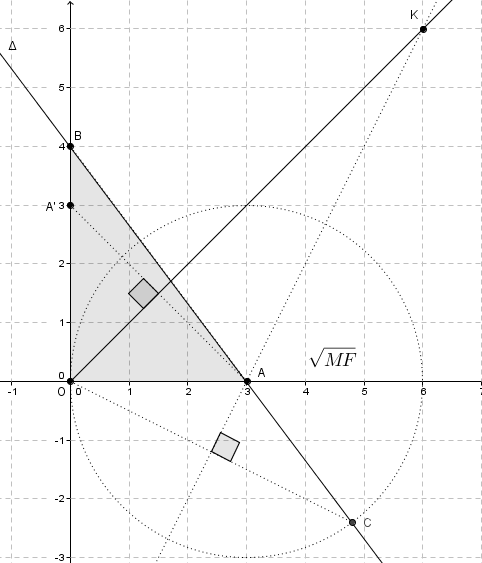
\includegraphics[scale=0.5]{de1.png}
\end{minipage}
\begin{minipage}{0.55\textwidth}
Ta có $x_C=\frac{24}5$, $C\in\Delta$ nên ta có tọa độ $C\left(-\frac{12}5;\frac{24}5\right)$.\\
Do $AO=AC$ nên $A$ nằm trên trung trực $d$ của $OC$. Với tọa độ $O,C$ đã biết ta tìm được $d$: $2x-y-6=0$.\\
Khi đó, $A=\Delta\cap d$ nên $A(3;0)$.\\
Ta có $K$ là tâm đường tròn bàng tiếp góc $O$ của tam giác $OAB$ nên $OK$ là phân giác góc $\goc{AOB}$. $OK$: $x-y=0$.\\
Gọi $A'$ là điểm đối xứng của $A$ qua $OK$, ta tìm được $A'(0;3)$ và $A'\in OB$. Do đó đường thẳng $OB$ chính là $Oy$ và ta tìm được $B(0;4)$.\\
\textit{\underline{Nhận xét}:} Với lời giải này ta thấy bài toán có một vài giả thiết thừa, chẳng hạn giả thiết tâm đường tròn bàng tiếp, giả thiết $C,B$ nằm khác phía so với $A$.
\end{minipage}

\deda{
 Cho $x\in \mathbb{R}$. Tìm GTNN của
$$ P=\dfrac{\sqrt{3(2x^2+2x+1)}}{3}+\dfrac{1}{\sqrt{2x^2+(3-\sqrt 3)x+3}}+\dfrac{1}{\sqrt{2x^2+(3+\sqrt 3)x+3}}. $$
}
\hda 
\bd với mỗi $x\in\mathbb{R}$ xét $A(x,x+1)$, $B\left(\frac{\sqrt 3}2;-\frac 12\right)$ và $C\left(-\frac{\sqrt 3}2;-\frac 12\right)$.\\
Khi đó ta có $P=\frac{OA}a+\frac{OB}b+\frac{OC}c$, trong đó $BC=a$, $CA=b$ và $AB=c$.\\
Gọi $G$ là trọng tâm $\Delta ABC$, ta có
$$ P=\frac{OA.GA}{a.GA}+\frac{OB.GB}{b.GB}+\frac{OC.GC}{c.GC}=\frac 32\left(\frac{OA.GA}{a.m_a}+\frac{OB.GB}{b.m_b}+\frac{OC.GC}{c.m_c}\right), $$
trong đó $m_a$, $m_b$, $m_c$ lần lượt là độ dài đường trung tuyến xuất phát từ $A,B,C$ của $\Delta ABC$.\\
Theo BĐT $AM-GM$, ta có
$$ a.m_a=\frac 1{2\sqrt 3}\sqrt{3a^2(2b^2+2c^2-a^2)}\le \frac 1{2\sqrt 3}\frac{3a^2+(2b^2+2c^2-a^2)}2=\frac{a^2+b^2+c^2}{2\sqrt 3}. $$
Bằng cách tương tự ta cũng có $b.m_b\le \frac{a^2+b^2+c^2}{2\sqrt 3}$ và $c.m_c\le \frac{a^2+b^2+c^2}{2\sqrt 3}$.\\
Suy ra $$P\ge \frac{3\sqrt 3}{a^2+b^2+c^2}(OA.GA+OB.GB+OC.GC).$$
Ta có $$OA.GA+OB.GB+OC.GC\ge \vt{OA}.\vt{GA}+\vt{OB}.\vt{GB}+\vt{OC}.\vt{GC}.$$
Mà
\begin{eqnarray*}
&&\vt{OA}.\vt{GA}+\vt{OB}.\vt{GB}+\vt{OC}.\vt{GC}\\
&=&\vt{OG}(\vt{GA}+\vt{GB}+\vt{GC})+GA^2+GB^2+GC^2\\
&=&\frac 49(m_a^2+m_b^2+m_c^2)=\frac{a^2+b^2+c^2}3
\end{eqnarray*}
Từ đó $P\ge 3$, đẳng thức xảy ra khi $x=0$. Vậy $P_{\min}=\sqrt 3$.
%Miễn bình luận.
\section{Đề 2}

\deda{
\bd cho hình vuông $ABCD$ có $M,N$ lần lượt là trung điểm của $BC$, $CD$. Tìm tọa độ $B, M$ biết $N(0;-2)$, đường thẳng $AM$ có phương trình $x+2y-2=0$ và cạnh hình vuông bằng $4$. 
}
\hda 
\begin{minipage}{0.5\textwidth}
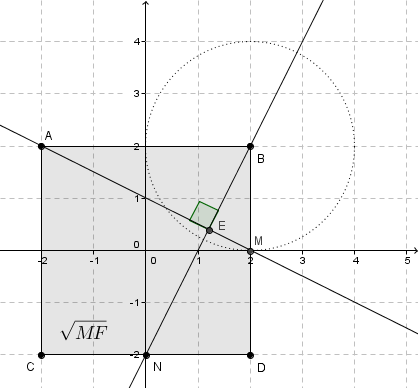
\includegraphics[scale=0.7]{de2-h1.png}
\end{minipage}
\begin{minipage}{0.5\textwidth}
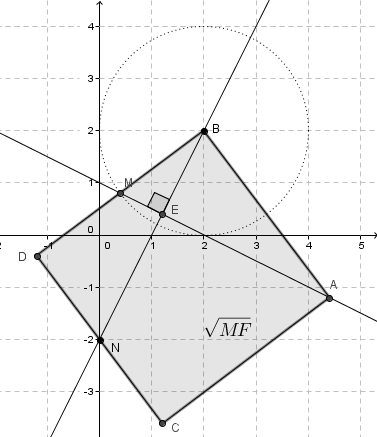
\includegraphics[scale=0.7]{de2-h2.png}
\end{minipage}
Chìa khóa của bài toán chính là tính chất $AM\bot BN$ (Tính chất này thường xuất hiện trong các đề thi đặc biệt thường xuất hiện với tư cách đáy của một hình chóp).\\
Trước hết $\Delta ABM\backsim \Delta BEM$ $(g.g)$ với $E=AM\cap BN$. Nên $AM\bot BN$.\\
Từ đó tìm được $BN$: $2x-y-2=0$ và $E\left(\frac 65;\frac 25\right)$.\\
Mặt khác ta cũng tính được $BE=\frac{4\sqrt 5}5$, $EN=\frac{6\sqrt 5}5$. Nên $\vt{EB}=-\frac 23\vt{EN}$, suy ra $B(2;2)$.\\
Lại có $BM=2$ nên $M$ thuộc đường tròn $(C)$ tâm $B$ bán kính $2$.
$(C)$: $(x-2)^2+(y-2)^2=4$.\\
$M=AM\cap (C)$ nên ta tìm được 2 điểm $M$ thỏa mãn: $M_1(2;0)$, $M_2\left(\frac 25;\frac 45\right)$.
\deda{
Giải hệ phương trình $\hpt{27x^3+3x+(9y-7)\sqrt{6-9y}=0\\ \frac 13x^2+y^2+\sqrt{2-3x}-\frac{109}{81}=0}$.
}
\hda 
Quan sát phương trình (1) của hệ ta thấy có thể độc lập thành hai phần, chỉ chứa $x$ và chỉ chứa $y$. Phần chứa $x$ có bậc $3$, phần chứa $y$ có dạng $u\sqrt{u}=(\sqrt{u})^3$ nên ta sẽ nghĩ đến việc dùng phương pháp hàm, với hàm đặc trưng là một hàm bậc 3.
 $$ (1)\iff  (3x)^3+3x=(6-9y)\sqrt{6-9y}+6-9y.\quad (\ast) $$
Dễ thấy hàm $f(t)=t^3+t$ đồng biến trên $\mathbb{R}$ nên
$$ (\ast)\iff  f(3x)=f(\sqrt{6-9y})\iff  3x=\sqrt{6-9y}\iff  \hpt{x\ge 0\\ y=\frac 23-x^2}. $$
Thế vào phương trình $(2)$ ta được $\frac 13 x^2+(\frac 23-x^2)^2+\sqrt{2-3x}-\frac{109}{81}=0$.\\
Vế trái của phương trình trên là hàm đồng biến trên $(0;\frac 23)$, lại thử thấy $x=\frac 13$ là một nghiệm nên hệ có nghiệm duy nhất $(\frac 13;\frac 59)$.

\deda{
 Tìm GTLN và GTNN của biểu thức $P=5^{2x}+5^y$, biết $x\ge 0$, $y\ge 0, x+y=1$.
}
\hda 
Ta có $x+y=1\iff  y=1-x$, nên $P=5^{2x}+\dfrac{5}{5^x}$.\\
Đặt $t=5^x$ thì $t\in [1;5]$. Xét $f(t)=t^2+\frac 5t$ với $t\in[1;5]$.\\
Ta tìm được $P_{\min}=f\left(\sqrt[3]{\frac 52}\right)=3\sqrt[3]{\frac{25}4}$, $P_{\max}=f(5)=26$.
\section{Đề 3}

\deda{
\bd hãy tính diện tích tam giác $ABC$ biết $H(5;5)$, $I(5;4)$ lần lượt là trực tâm và tâm đường tròn ngoại tiếp tam giác $ABC$ và cạnh $BC$ nằm trên đường thẳng $x+y-8=0$.
}
\hda 
\begin{minipage}{0.43\textwidth}
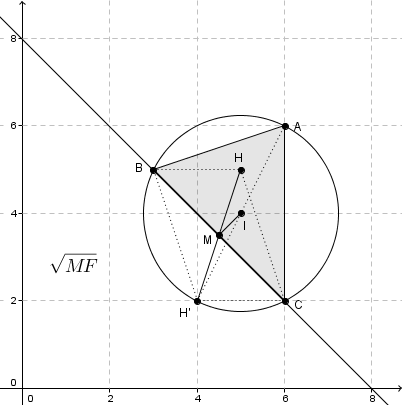
\includegraphics[scale=0.7]{de3.png}
\end{minipage}
\begin{minipage}{0.56\textwidth}
Đây là một dạng hình rất quen thuộc đối với các bạn lớp 9. Nói như thế để thấy rằng các bạn có kiễn thức hình phẳng lớp 9 tốt thì sẽ có lợi thế lớn trong chủ đề này.\\
Gọi $M$ là hình chiếu của $I$ lên $BC$, thì $M\left(\frac 92;\frac 72\right)$ và $M$ là trung điểm $BC$.\\
Gọi $H'$ là điểm đối xứng của $H$ qua $M$, thì $H'(2;4)$ và tứ giác $HBH'C$ là hình bình hành.\\
Do đó $H'C\parallel BH$, mà $BH\bot AC$ nên $\goc{ACH'}=90^o$, tương tự cũng có $\goc{ABH'}=90^o$. Suy ra tứ giác $ABH'C$ nội tiếp đường tròn đường kính $AH'$.
\end{minipage}\\
Từ đó $I$ là trung điểm của $AH'$, suy ra $A(6;6)$.\\
Lại có $BC=2MC=2\sqrt{R^2-MI^2}=3\sqrt 2$. Và $S_{\Delta ABC}=\frac 12d(A, BC).BC=6$.\\
\textit{\underline{Nhận xét}:} Ta có thể lấy điểm phụ $H'$ khác là giao của $AH$ với đường tròn ngoại tiếp tam giác.
\deda{
 Giải phương trình $(x-\ln x)\sqrt{2x^2+2}=x+1$.
}
\hda 
Đk: $x>0$. phương trình tương đương với $x-\ln x=\dfrac{x+1}{\sqrt{2x^2+2}}$.\quad $(\ast)$\\
Bằng cách xét hàm ta sẽ chỉ ra được $(\ast)$ có $VT\le 1$ và $VP\ge 1$, đẳng thức đều xảy ra khi $x=1$.\\
Vậy phương trình có nghiệm duy nhất $x=1$.

\deda{
Cho $0<x<y<z$. Tìm GTNN
$$ P=\dfrac{x^3z}{y^2(xz+y^2)}+\dfrac{y^4}{z^2(xz+y^2)}+\dfrac{z^3+15x^3}{x^2z}. $$
}
\hda 
Đặt $a=\frac xy$, $b=\frac yz$, $c=\frac zx$, suy ra $abc=1$, $c>1$ và
$$ P=\frac{\left(\frac xy\right)^3}{\frac xy+\frac yz}+\frac{\left(\frac yz\right)}{\frac xy+\frac yz}+\left(\frac zx\right)^2+\frac{15}{\frac zx}=\frac{a^3}{a+b}+\frac{b^3}{a+b}+c^2+\frac{15}c. $$
Ta có $a^3+b^3\ge ab(a+b)\implies  \frac{a^3}{a+b}+\frac{b^3}{a+b}\ge ab=\frac 1c$. Suy ra $P\ge \frac 1c+c^2+\frac{15}c=c^2+\frac{16}c$.\\
Xét $f(c)=c^2+\frac{16}c$ với $c\in (1;+\infty)$ ta được $f(c)\ge f(2)=12$.\\
Vậy $P_{\min}=12$ khi $z=\sqrt 2y=2x$.
\section{Đề 4}

\deda{
Giải hệ phương trình $\hpt{\sqrt{2x-y-1}+\sqrt{3y+1}=\sqrt x+\sqrt{x+2y}\\ x^3-3x+2=2y^3-y^2}.$
}
\hda 
Đk: $\hpt{2x\ge y+1\\ y\ge -\frac 13\\x\ge 0\\  x+2y\ge 0}\iff  \hpt{y\ge -\frac 13\\ x\ge \frac 13\\x+2y\ge 0}$.\\
Ở phương trình (1), quan sát các biểu thức dưới căn (hoặc sử dụng Casio), ta sẽ tìm được mối liên hệ giữa các biến định hướng cho các biến đổi sau
$$ (1)\iff  (\sqrt{2x-y-1}-\sqrt x)-(\sqrt{x-2y}-\sqrt{3y-1})=0$$
$$\iff  \dfrac{x-y-1}{\sqrt{2x-y-1}+\sqrt x}-\dfrac{x-y-1}{\sqrt{x-2y}+\sqrt{3y-1}}=0$$
$$\iff  \hoac{x-y-1=0\quad (3)\\ \sqrt{2x-y-1}+\sqrt x=\sqrt{x-2y}-\sqrt{3y-1}\quad (4)}. $$
$(3)\iff  y=x-1$ thế vào $(2)$ ta được phương trình bậc 3 ẩn $x$ có hai nghiệm $x=1$, $x=5$. Suy ra nghiệm hệ $(1;0)$ và $(5;4)$.\\
Với phương trình $(4)$, làm tương tự với $(1)$ ta sẽ có biến đổi
$$ (4)\iff  (\sqrt{2x-y-1}-\sqrt{x+2y})+(\sqrt x-\sqrt{3y-1})=0$$
$$\iff  \hoac{x-3y-1=0\\ \dfrac{1}{\sqrt{2x-y-1}+\sqrt{x+2y}}+\dfrac{1}{\sqrt x+\sqrt{3y-1}}=0\quad \textit{(Vô nghiệm)}} $$
Với $x-3y-1=0$ thế vào $(2)$ ta cũng sẽ tìm được $x=1$. Vậy hệ có hai nghiệm  $(1;0)$; $(5;4)$.

\deda{
\bd cho hình vuông $ABCD$ có tâm $I\left(\frac 72;\frac 32\right)$. Điểm $M(6;6)\in AB$ và $N(8;-2)\in BC$. Tìm tọa độ các đỉnh của hình vuông.
}
\hda 
\begin{minipage}{0.43\textwidth}
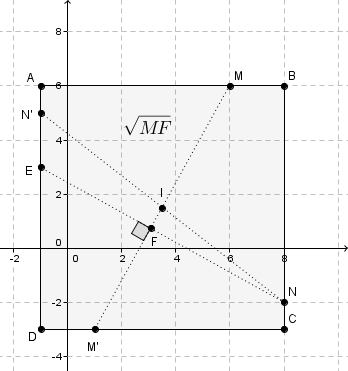
\includegraphics[scale=0.7]{de4.png}
\end{minipage}
\begin{minipage}{0.56\textwidth}
Ta tìm được tọa độ $M'(1;-3)$ đối xứng với $M$ qua $I$, $N'(-1;5)$ đối xứng với $N$ qua $I$.\\
Gọi $F$ là hình chiếu của $N$ lên $MM'$, do đã biết tọa độ $N$, viết được phương trình $MM'$ nên ta tìm được tọa độ $F\left(\frac{163}{53};\frac{39}{53}\right)$.\\
Mặt khác, ta lại chứng minh được $NE=MM'$ ($\Delta MM'P=\Delta NEQ$, với $P$ là hình chiếu của $M$ lên $CD$, $Q$ là hình chiếu của $N$ lên $AD$.).\\
Từ đó ta có $\vt{NF}=\frac{NF}{MM'}\vt{NE}$, do độ dài $NF$, $MM'$ tính được, tọa độ $N,F$ đã biết nên ta sẽ suy ra tọa độ $E(-1;3)$.\\
\end{minipage}\\
Khi đó ta viết được phương trình $AD$ (qua $E,N'$); phương trình $AB$, $CD$ ( lần lượt qua $M$, $M'$ vuông góc với $AD$) và tìm được tọa độ $A(-1;6)$, $D(-1;-3)$. Do $I$ là trung điểm $AC$, $BD$ nên cũng tìm được $C(8;-3)$, $B(8;6)$.
\deda{
Cho $x,y,z\in (0;1)$ thỏa mãn $(x^3+y^3)(x+y)=xy(1-x)(1-y)$. Tìm GTLN
$$ P=\dfrac{1}{\sqrt{1+x^2}}+\dfrac{1}{\sqrt{1+y^2}}+3xy-(x^2+y^2). $$
}
\hda 
Ta có $$ (x^3+y^3)(x+y)=xy(1-x)(1-y)\iff  \left(\frac{x^2}y+\frac{y^2}x\right)(x+y)=(1-x)(1-y). $$
Mà $\left(\frac{x^2}y+\frac{y^2}x\right)(x+y)\ge 4xy$ và $(1-x)(1-y)=1-(x+y)+xy\le 1-2\sqrt{xy}+xy$.\\
Suy ra $$1-2\sqrt{xy}+xy\ge 4xy\iff  0<xy\le\frac 19.$$
Mặt khác $\frac{1}{1+x^2}+\frac{1}{1+y^2}\le \frac{2}{1+xy}$ với $x,y\in (0;1)$. Suy ra
$$ \frac{1}{\sqrt{1+x^2}}+\frac{1}{\sqrt{1+y^2}}\le \sqrt{2\left(\frac{1}{1+x^2}+\frac{1}{1+y^2}\right)}\le\sqrt{2\left(\frac{2}{1+xy}\right)}=\frac{2}{\sqrt{1+xy}}. $$
Lại có $3xy-(x^2+y^2)=xy-(x-y)^2\le xy$. Suy ra $ P\le \frac{2}{\sqrt{1+xy}}+xy$.\\
Xét $f(t)=\frac{2}{\sqrt{1+t}}+t$ với $t\in\left(0;\frac 19\right]$. Ta tìm được $P_{\max}=f(\frac 19)=\frac{6\sqrt{10}}{10}+\frac 19$.
\section{Đề 5}

\deda{
\bd cho tam giác $ABC$ có trực tâm $H(-1;3)$, tâm đường tròn ngoại tiếp $I(-3;3)$, chân đường cao kẻ từ đỉnh $A$ là điểm $K(-1;1)$. Tìm tọa độ $A,B,C$.
}
\hda 
Ta có thể viết được phương trình $BC$ (qua $K$ vuông góc với $KH$) là $y-1=0$. Đến đây bạn đọc có thể tham khảo hướng dẫn giải ở \textbf{Đề 3} để tìm ra lời giải.\\
Ta tìm được $\{A(-1;7), B(1;1), (-7;1)\}$ hoặc $\{A(-1;7), B(-7;1), (1;1)\}$.

\deda{
Giải hệ phương trình $\hpt{x^2(x-3)-y\sqrt{y+3}=-2\\ 3\sqrt{x-2}=\sqrt{y(y+8)}}$.
}
\hda 
Đk: $x\ge 2$; $y\ge 0$\\
Quan sát $(1)$ ta cũng sẽ định hướng được sẽ sử dụng phương pháp hàm số, với hàm đặc trưng sẽ là một hàm bậc 3.
$$ (1)\iff  (x-1)^3-3(x-1)=(y+3)\sqrt{y+3}-3\sqrt{y+3}.\quad (\ast) $$
Dễ thấy hàm $f(t)=t^3-3t$ đồng biến trên $[1;+\infty)$ nên
$$ (\ast)\iff  f(x-1)=f(\sqrt{y+3})\iff  x-1=\sqrt{y+3} $$
Khi đó,
$$ (2)\iff  9(x-2)=y^2+8y\iff  9(\sqrt{y+3}-1)=y^2+8y\quad (\ast\ast) $$
Nhẩm (hoặc sử dụng Casio) tìm được nghiệm $y=1$ nên bằng phương pháp nhân liên hợp ta sẽ biến đổi được như sau
$$ (\ast\ast)\iff  (y-1)\left(\dfrac{9}{\sqrt x{y+3}+2}-y-9\right)=0\iff  y=1. $$
(Vì với $y\ge 0$ thì $\dfrac{9}{\sqrt x{y+3}+2}-y-9<0$). Vậy hệ có nghiệm $(3;1)$.

\deda{
Cho $x,y,z\in \mathbb{R}$ thỏa mãn $x^2+y^2+z^2=9$, $xyz\le 0$. CMR $2(x+y+z)-xyz\le 10$.
}
\hda 
Không giảm tính tổng quát, giả sử $x\le y\le z$, do $xyz\le 0$ nên $x\le 0$. Lại có $x^2+y^2+z^2=9$ nên $x^2\le 9$, suy ra $x\in [-3;0]$.\\
Mặt khác $yz\le \left(\frac{y+z}2\right)^2\le \frac{y^2+z^2}2$. Do đó 
\begin{eqnarray*}
&&2(x+y+z)-xyz\\ 
&=& 2x+2(y+z)-xyz\\
&\le & 2x+2\sqrt{2(y^2+z^2)}-x\cdot \frac{y^2+z^2}2\\
&=&\frac 12x^3-\frac 52 x+2\sqrt{2(9-x^2)}=f(x).
\end{eqnarray*}
Xét $f(x)$ trên $[-1;0]$ ta sẽ chỉ ra điều phải chứng mình. Đẳng thức xảy ra khi $x=-1, y=z=2$.
\section{Đề 6}

\deda{
\bd cho tam giác $ABC$ có tâm đường tròn ngoại tiếp là $I(-2;1)$ và thỏa mãn điều kiện $\goc{AIB}=90^o$, chân đường cao kẻ từ $A$ đến $BC$ là $D(-1;-1)$, đường thẳng $AC$ đi qua $M(-1;4)$. Tìm tọa độ $A,B$ biết $A$ có hoành độ dương.
}
\hda 
\begin{minipage}{0.43\textwidth}
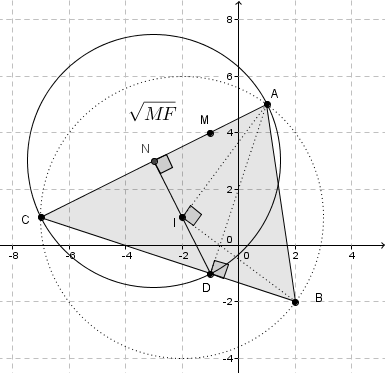
\includegraphics[scale=0.7]{de6.png}
\end{minipage}
\begin{minipage}{0.56\textwidth}
Chìa khóa của bài toán là có lẽ là phát hiện ra mối liên hệ giữa 3 giả thiết bài toán đã cho: $DI\bot AC$ ($M\in AC$). Việc định hướng được tính chất này cũng khá tự nhiên, nhưng cần kiến thức hình lớp 9 vững, đây cũng là xu hướng ra đề thường gặp.\\
Ta có $\goc{AIB}=90^o$ nên $\goc{ACB}=45^o$ (Góc nội tiếp bằng $\frac 12$ góc ở tâm cùng chắn cung). Do đó $\Delta ACD$ vuông cân tại $D$, suy ra $DA=DC$, mà $IA=IC$ nên $DI$ là đường trung trực của $AC$.\\
Từ đó, $ID\bot AC$ và $N$ là trung điểm $AC$ với $N$ là hình chiếu vuông góc của $I$ lên $AC$.
\end{minipage}\\
Ta tìm được $AC$: $x-2y+9=0$ (qua $M$ vuông góc với $DI$) và $N(-3;3)$. Ta cũng viết được phương trình đường tròn $(C)$: $(x+3)^2+(y-3)^2=20$ tâm $N$ bán kính $ND$. Suy ra $A(1;5)=(C)\cap AC$ (chú ý, hoành độ $A$ dương) và cũng sẽ tìm được $B(2;-2)$.
\deda{
Giải BPT $3(x^2-2)+\dfrac{4\sqrt 2}{\sqrt{x^2-x+1}}>\sqrt x(\sqrt{x-1}+3\sqrt{x^2-1})$.
}
\hda 
Đk: $x\ge 1$, ta biến đổi phương trình trở thành
$$ 3(\sqrt{x^2-1}-\sqrt{x})^2+(\sqrt{x^2-x}-1)^2+2\left(\dfrac{4\sqrt 2}{\sqrt{x^2-x+1}}+x^2-x-5\right)>0.\quad (\ast) $$
Xét hàm $f(t)=\dfrac{4\sqrt 2}{t}+t^2-6$ với $t=\sqrt{x^2-x+1}\ge 1$.\\ Ta có $f'(t)=2t-\dfrac{4\sqrt 2}{t^2}=\dfrac{2(t^3-2\sqrt 2)}{t^2}$,\quad $f'(t)=0\iff  t=\sqrt 2$.\\
Lập bảng biến thiên và ta sẽ chỉ ra được $f(t)\ge 0$ với mọi $t\ge 1$.\\
Đẳng thức xảy ra khi $t=\sqrt 2\iff  x=\dfrac{1+\sqrt 5}2$.\\
Từ đó ta có $(\ast)\iff  \hoac{\sqrt{x^2-1}-\sqrt x\neq 0\\ \sqrt{x^2-x}-1\neq 0\\ \dfrac{4\sqrt 2}{\sqrt{x^2-x+1}}+x^2-x-5\neq 0}\iff  x\neq \dfrac{1+\sqrt5}{2}$.\\
Vậy tập nghiệm của phương trình là $S=[1;+\infty)\setminus\left\{\dfrac{1+\sqrt 5}2\right\}$.
%Nhận xét: Bài tập như dở hơi -_-

\deda{
Xét các số thực dương $x,y,z$ thỏa mãn điều kiện $2(x+y)+7z=xyz$. Tim GTNN $S=2x+y+2z$.
}
\hda 
Ta có $2(x+y)=z(xy-7)$. Do $x,y,z$ là các số dương nên $xy-7>0$, suy ra $z=\frac{2(x+y)}{xy-7}$.\\
Suy ra $S=f(x,y)=2x+y+\frac{4(x+y)}{xy-7}$ với điều kiện $x>0$, $y>0$, $xy>7$.\\
Với mỗi $x$ cố định, xét đạo hàm của $f(x,y)$ theo ẩn $y$ ta được:
$$ f'_y(x,y)=1+\frac{4(xy-7)-4x(x+y)}{(xy-7)^2}=1-\frac{28+4x^2}{(xy-7)^2}. $$
Khi đó, $f'_y(x,y)=0\iff  x^2y^2-14xy+21-4x^2=0\iff  y_o=\frac 7x+2\sqrt{1+\frac 7{x^2}}$.\\
Suy ra $$f(x,y)\ge f(x,y_o)=2x+\frac{11}x+4\sqrt{1+\frac 7{x^2}}=g(x).$$
Xét $g(x)$ với $x\in (0;+\infty)$ ta sẽ tìm được $S\ge f(x;y_o)=g(x)\ge 15$.\\
Vậy $S_{\min}=15$ khi $x=3$, $y=5$, $z=2$.
\section{Đề 7}

\deda{
\bd cho hình bình hành $ABCD$ có $N$ là trung điểm $CD$ và $BN$ có phương trình $13x-10y+13=0$; điểm $M(-1;2)$ thuộc đoạn thẳng $AC$ sao cho $AC=4AM$. Gọi $H$ là điểm đối xứng của $N$ qua $C$. Tìm tọa độ $A,B,C,D$ biết $3AC=2AB$ và $H\in \Delta: 2x-3y=0$.
}
\hda 
\begin{minipage}{0.47\textwidth}
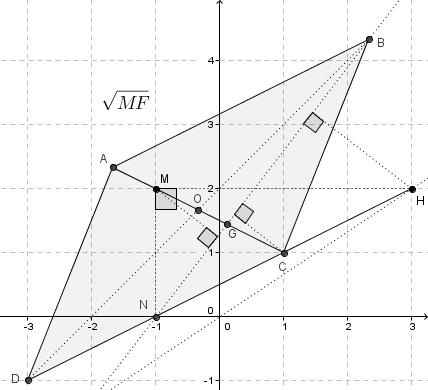
\includegraphics[scale=0.7]{de7.png}
\end{minipage}
\begin{minipage}{0.5\textwidth}
Gọi $G=BN\cap AC$ thì $G$ là trọng tâm tam giác $BCD$, suy ra $GC=\frac 13AC$. Mà $AC=4AM$ nên $MG=\frac 5{12}AC$, suy ra $CG=\frac 45MG$.
Từ đó $$d(C, BN)=\frac 45d(M,BN).$$
Lại có $HN=2CN$ nên $$d(H,BN)=2d(C,BN)=\frac 85d(M,BN).$$
Mà $d(M,BN)=\frac{20}{\sqrt{269}}$ và $H(3t,2t)$ (do $H\in\Delta$). Nên ta sẽ tìm được $t=1$, $t=-\frac{45}{19}$.
\end{minipage}\\
Để ý rằng $M, H$ nằm khác phía so với $BN$ nên ta chỉ ra được $H(3;2)$.\\
Mặt khác với giả thiết $3AC=2AB=2CD=2NH$ ta chỉ ra được $MC=\frac 12NH$ tức là tam giác $MNH$ vuông tại $M$ và tìm được $N(-1;0)$.\\
Từ đó ta sẽ tìm được $C(1;1)$, $D(-3;-1)$, $A\left(-\frac 53;\frac 73\right)$, $B\left(\frac 73;\frac{13}3\right)$.

\deda{
Giải hệ phương trình $\hpt{x^2+(y^2-y-1)\sqrt{x^2+2}-y^3+y+2=0\\ \sqrt[3]{y^2-3}-\sqrt{xy^2-2x-2}+x=0}.$
}
\hda 
Đk: $xy^2-2x-2\ge 0$.\\
Trong phương trình $(1)$, đặt $\sqrt{x^2+2}=t\ge 2$ ta được
$$ t^2+(y^2-y-1)t-y^3+y=0.\quad (\ast) $$
Do $\Delta_t=(y^2+y-1)^2$ (hoặc sử dụng Casio) nên
$$ (\ast)\iff \hoac{t=y\\ t=1-y^2\le 1\,\,\textit{(loại)}}\iff \hpt{y\ge 2\\ y^2=x^2+2}. $$
Thế vào $(2)$ ta được
$$ \sqrt[3]{x^2-1}-\sqrt{x^3-2}+x=0\quad\quad\text{(Đk: $x\ge\sqrt[3]{2}$).} $$
Bằng phương pháp nhân với lượng liên hợp ta sẽ chỉ ra được phương trình trên có đúng 1 nghiệm $x=3$.
\deda{
Cho $a\in[1;2]$. CMR $(2^a+3^a+4^a)(6^a+8^a+12^a)<24^{a+1}$.
}
\hda 
Bất đẳng thức tương đương với $$ (2^a+3^a+4^a)\left(\frac 1{2^a}+\frac 1{3^a}+\frac 1{4^a}\right)<24. $$
Do $a\in[1;2]$ nên $2\le 2^a\le 4$; $3\le 3^a\le 9$; $4\le 4^a\le 16$ $\implies $ $2\le 2^a<16$; $2<3^a<16$; $2<4^a\le 16$.\\
Lại có, $x\in[2;16]$ thì $(x-2)(x-16)\le 0\iff  x^2-18x+32\le 0\iff  x-18+\frac{32}x\le 0\iff  \frac{32}x\le 18-x$.\\
Từ đó suy ra
$$ 32\left(\frac 1{2^a}+\frac 1{3^a}+\frac 1{4^a}\right)<54-(2^a+3^a+4^a)\iff   \frac 1{2^a}+\frac 1{3^a}+\frac 1{4^a}<\frac{54-(2^a+3^a+4^a)}{32}.$$
Khi đó
\begin{eqnarray*}
(2^a+3^a+4^a)\left(\dfrac 1{2^a}+\dfrac 1{3^a}+\dfrac 1{4^a}\right)&<&\dfrac{(2^a+3^a+4^a)[54-(2^a+3^a+4^a)]}{32}\\ 
& \le & \dfrac{1}{32}\left[\dfrac{[2^a+3^a+4^a+54-(2^a+3^a+4^a)]}{2}\right]^2=\dfrac{729}{32}<24.
\end{eqnarray*}
\section{Đề 8}

\deda{
\bd cho hình bình hành $ABCD$ có $\goc{ABC}$ nhọn, $A(-2;-1)$. Gọi $H,K,E$ lần lượt là hình chiếu vuông góc của $A$ trên các đường thẳng $BC, BD, CD$. Đường tròn $(C):$ $x^2+y^2+x+4y+3=0$ ngoại tiếp tam giác $HKE$. Tìm tọa độ $B,C,D$ biết $H$ có hoành độ âm, $C$ có hoành độ dương và nằm trên đường thẳng $x-y-3=0$.
}
\hda 
\begin{minipage}{0.47\textwidth}
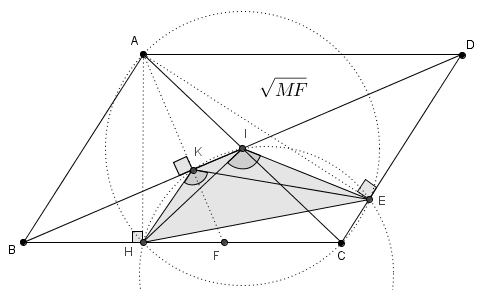
\includegraphics[scale=0.6]{de8.png}
\end{minipage}
\begin{minipage}{0.52\textwidth}
Gọi $I=AC\cap BD$, ta sẽ chứng minh $I\in (C)$ bằng cách chỉ ra $HKIE$ là tứ giác nội tiếp. Thật vậy, $AHCE$ nội tiếp đường tròn tâm $I$ nên $\goc{HIE}=2\goc{HAE}$ (góc ở tâm và góc nội tiếp cùng chắn 1 cung).\\
Lại có $ABHK, AKED$ là các tứ giác nội tiếp và $\goc{EAB}=\goc{HAD}=90^o$ nên 
\end{minipage}
$$\goc{HKE}=180^o-\goc{HKB}-\goc{EKD}=180^o-\goc{HAB}-\goc{EAD}=90^o-\goc{HAB}+90^o-\goc{EAD}=2\goc{HAE}.$$
Từ đó, $\goc{HKE}=\goc{HIE}$, tức là $HKIE$ nội tiếp.\\
Mặt khác, $I$ là trung điểm $AC$ và $C(c;c-3)\in d$ $(c>0)$ nên $I\left(\frac{c-2}2;\frac{c-4}2\right)$. Do $I\in (C)$ nên ta tìm được $c=2$ và $I(0;-1)$, $C(2;-1)$.\\
Gọi $(C')$ là đường tròn đường kính $AC$, $(C')$: $x^2+(y+1)^2=4$.\\
$E,H=(C)\cap (C')$ nên ta sẽ tìm được $\left(-\frac 85;-\frac{11}5\right)$, $E(0;-3)$ (Do $H$ có hoành độ âm). \\
Từ đó ta cũng tìm được $B(-4;-3)$, $C(2;-1)$, $D(4;1)$.
\deda{
Giải hệ phương trình $\hpt{3\sqrt{y^3(2x-y)}+\sqrt{x^2(5y^2-4x^2)}=4y^2\quad (1)\\ \sqrt{2-x}+\sqrt{y+1}+2=x+y^2\quad (2)}$.
}
\hda 
Đk: $x\le 2$; $y\ge -1$; $y^3(2x-y)\ge 0$; $5y^2-4x^2\ge 0$.\\
Nhận thấy $(1)$ đồng bậc $3$ nên đặt $y=tx$. Ta có $y^3(2x-y)\ge 0\implies  xy\ge 0\implies  t> 0$.\\
Ta sẽ được phương trình
$$ 3\sqrt{t^3(2-t)}+\sqrt{5t^2-4}=4t^2. $$
Bằng phương pháp nhân với lượng liên hợp với nhân tử chung là $(t-1)^2$ ta xác định được $(\ast)$ có đùng một nghiệm $t=1$, tức là $x=y$. (Bằng BĐT AM-GM ta cũng sẽ chỉ ra được $x=y$).\\
Thế vào $(2)$ ta được
$$ \sqrt{2-x}+\sqrt{x+1}+2=x+x^2. $$
Suy ra $x^2+x-2>0\implies  x>1$. Bằng phương pháp nhân liên hợp ta sẽ phân tích phương trình trở thành
$$ (x^2-x-1)\left(1+\dfrac{1}{x-1+\sqrt{2-x}}+\dfrac{1}{x+\sqrt{x+1}}\right)=0 $$
$$ \iff  x^2-x-1=0\implies  x=y=\dfrac{1+\sqrt{5}}2. $$
\deda{
Cho $a,b,c>0$ thỏa mãn $4(a^3+b^3)+c^3=2(a+b+c)(ac+bc-2)$. Tìm GTLN
$$ P=\dfrac{2a^2}{3a^2+b^2+2a(c+2)}+\dfrac{b+c}{a+b+c+2}-\dfrac{(a+b)^2+c^2}{16}. $$
}
\hda 
Ta có $x^3+y^3\ge \frac 14(x+y)^3$; $xy\le \left(\frac{x+y}2\right)^2$ với mọi $x,y>0$. Suy ra
$$ \frac 14(a+b+c)^3\le (a+b)^3+c^3\le 4(a^3+b^3)+c^3\le 2(a+b+c)\left(\frac{(a+b+c)^2}4-2\right) $$
Suy ra $a+b+c\ge 4$.\\
Khi đó áp dụng BĐT AM-GM ta có
$$ \frac{2a^2}{3a^2+b^2+2a(c+2)}=\frac{a}{a+c+2+\left(\frac{b^2}{2a}+\frac a2\right)}\le \frac{a}{a+c+2+2\sqrt{\frac{b^2}{2a}\cdot\frac a2}}=\frac a{a+b+c+2}, $$
và $(a+b)^2+c^2\ge \frac 12(a+b+c)^2$. Suy ra $$P\le \frac{a+b+c}{a+b+c+2}-\frac{(a+b+c)^2}{32}=\frac{t}{t+2}-\frac{t^2}{32}.$$
Với $t=a+b+c\ge 4$, ta có $f'(t)=\frac{2}{(t+2)^2}-\frac{t}{16}=\frac{32-t(t+2)^2}{16(t+2)^2}<0$, $\forall t\ge 4$.\\
Suy ra $f(t)$ nghịch biến trên $[4;+\infty)$. Do đó $P\le f(t)\le f(4)=\frac 16$.\\
Dấu bằng xảy ra khi $\hpt{a=b,a+b=c\\ a+b+c=4}\iff  a=b=1,c=2$. Vậy $P_{\max}=\frac 16$.
\section{Đề 9}

\deda{
Giải hệ phương trình $\hpt{\sqrt{x+2y+1}-2x=4(y-1)\quad (1)\\ x^2+4y^2+2xy=7\quad (2)}$.
}
\hda 
Đây là một hệ phương trình khá đơn giản.\\
Với $(1)$, đặt $\sqrt{x+2y+1}=t$, ta sẽ giải được $t=2$. Thế vào $(2)$ ta tìm được nghiệm của hệ là $(1;1)$ và $(1;\frac 12)$.

\deda{
\bd cho tam giác $ABC$ có phương trình đường thẳng $AB$: $2x+y-1=0$, phương trình $AC:$, $3x+4y+6=0$ và điểm $M(1;-3)$ nằm trên $BC$ thỏa mãn $3MB=2MC$. Tìm tọa độ trọng tâm $G$ của tam giác $ABC$.
}
\hda 
Một bài tập khá đơn giản minh họa cho phương pháp tham số hóa.\\
$A=AB\cap AC$ nên $A(2;-3)$. $B\in AB$ nên $B(b;1-2b)$, $C\in AC$ nên $C(-2-4c;3c)$.\\
 Một điểm lưu ý là $M$ chưa biết nằm trong hay nằm ngoài $B,C$ nên ta cần xét 2 trường hợp\\
\textbf{TH1}: $M$ nằm ngoài, tức là $3\vt{MB}=2\vt{MC}$ ta tìm được $b=\frac{11}5$, $c=-\frac 65$. Từ đó $G\left(\frac 73;-\frac{10}3\right)$.\\
\textbf{TH2}: $3\vt{MB}=-2\vt{MC}$ ta cũng xác định được $G\left(1;-\frac 83\right)$.

\deda{
Tìm tất cả các giá trị của $m$ để bất phương trình sau có nghiệm trên $[0;2]$
$$ \sqrt{(m+2)x+m}\ge |x-1|. $$
}
\hda 
Với $x\in [0;2]$ ta có $$\sqrt{(m+2)x+m}\ge |x-1|\iff  (m+2)x+m\ge (x-1)^2\iff  m\ge \frac{x^2-4x+1}{x+1}=f(x).$$
Xét $f(x)$ trên $[0;2]$ ta chỉ ra được $f(x)\in [2\sqrt 6-6;1]$.\\
Do đó để BPT có nghiệm trên $[0;2]$ thì $m\ge 2\sqrt 6-6$.
\section{Đề 10}

\deda{
\bd cho hình vuông $ABCD$ có $A(-1;2)$. Gọi $M, N$ lần lượt là trung điểm của $AD$ và $DC$; $K=BN\cap CM$. Viết phương trình đường tròn ngoại tiếp tam giác $BMK$, biết $BN$ có phương trình $2x+y-8=0$ và điểm $B$ có hoành độ lớn hơn $2$. 
}
\hda 
\begin{minipage}{0.3\textwidth}
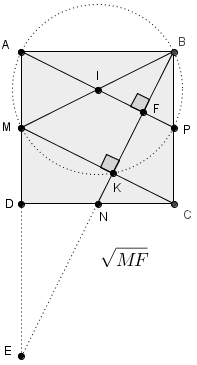
\includegraphics[scale=0.9]{de10.png}
\end{minipage}
\begin{minipage}{0.68\textwidth}
Một lần nữa, chúng ta lại bắt gặp tính chất hình học ở \textbf{Đề 2}, tuy nhiên cần phải tận dụng nó một cách khéo léo kết hợp với các giả thiết khác.\\
Tương tự như ở \textbf{Đề 2}, ta chứng minh được $CM\bot BN$ và $AP\bot BN$ với $P$ là trung điểm $BC$. Và do đó, $I=AP\cap BM$ là tâm của đường tròn ngoại tiếp $\Delta BKM$ có đường kính $BM$.\\
Mặt khác, gọi $F=AP\cap BN$ ta có $AF=d(A,BN)=\frac8{\sqrt 5}$.\\
Gọi $E=AD\cap BN$, dễ thấy $D$ là trung điểm $AE$. Lại có $$\frac 1{AF^2}=\frac 1{AB^2}+\frac{1}{AE^2}=\frac 5{4AB^2}.$$
Nên $AB=4$. Từ đó ta tính được $IA=\frac{AP}2=\sqrt 5$, suy ra $\vt{AI}=\frac 58\vt{AF}$. Ta lại tìm được $F\left(\frac{11}5;\frac{18}5\right)$ (Hình chiếu của $A$ lên $BN$) nên ta cũng tính được $I(1;3)$. Và phương trình cần tìm là $(x-1)^2+(y-3)^2=5$.
\end{minipage}

\textit{\underline{Nhận xét}:} Cách làm trong đáp án chính thức cần tìm tọa độ điểm $B$ từ giả thiết $AB=4$ và $B\in BN$ nên cần $x_B>2$ để loại nghiệm. Nhưng với cách làm này ta thấy giả thiết $x_B>2$ bị thừa.


\deda{
Giải hệ phương trình $\hpt{(1-y)\sqrt{x^2+2y^2}=x+2y+3xy\quad (1)\\ \sqrt{y+1}+\sqrt{x^2+2y^2}=2y-x\quad (2)}$.
}
\hda 
Đk: $y\ge -1$. Với phương trình $(1)$, đặt $\sqrt{x^2+2y^2}=t\ge 0$, coi là phương trình ẩn $t$, $x,y$ là tham số. Ta tính được $\Delta_t=(2x+3y+1)^2$ nên
$$(1)\iff  \hoac{\sqrt{x^2+2y^2}=-x-y-1\\ \sqrt{x^2+2y^2}=x+2y}$$
Thế vào $(2)$ ta được nghiệm $\left(\dfrac{-1-\sqrt 5}4;\dfrac{1+\sqrt 5}2\right)$.
% Nx: Bài toán mang tính chất đánh đố.
\deda{
Cho $x,y,z>0$ thỏa mãn $5(x^2+y^2+z^2)=9(xy+2yz+zx)$. Tìm GTLN
$$ P=\dfrac{x}{y^2+z^2}-\dfrac{1}{(x+y+z)^3}. $$
}
\hda 
Ta có $5x^2+5(y^2+z^2)=9x(y+z)+18yz\iff  5x^2-9x(y+z)=18yz-5(y^2+z^2)$.\\
Lại có $yz\le \frac 14(y+z)^2$; $y^2+z^2\ge \frac 12(y+z)^2$ nên $18yz-5(y^2+z^2)\le 2(y+z)^2$.\\
Do đó
\begin{eqnarray*}
&&5x^2-9x(y+z)\le 2(y+z)^2\\ 
&\iff  & [x-2(y+z)](5x+y+z)\le 0\\
&\iff  & x\le 2(y+z). 
\end{eqnarray*}
Và
$$ P=\frac{x}{y^2+z^2}-\frac{1}{(x+y+z)^3}\le \frac{2x}{(y+z)^2}-\frac 1{(x+y+z)^3}\le \frac 4{y+z}-\frac 1{27(y+z)^3}. $$
Đặt $y+z=t>0$ ta có $P\le 4t-\frac 1{27}t^3=f(t)$. Xét $f(t)$ ta suy ra được $P\le 16$.\\
Vậy $P_{\max}=16$ khi $x=\frac 13$; $y=z=\frac 1{12}$.
\section{Đề 11}

\deda{
\bd cho hình thang $ABCD$ có đáy lớn $CD=2AB$, điểm $C(-1;-1)$, trung điểm của $AD$ là $M(1;-2)$. Tìm tọa độ $B$, biết diện tích tam giác $BCD$ bằng $8$, $AB=4$ và $D$ có hoành độ nguyên dương.
}
\hda 
\begin{minipage}{0.4\textwidth}
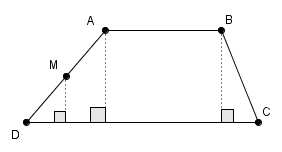
\includegraphics[scale=0.9]{de11.png}
\end{minipage}
\begin{minipage}{0.58\textwidth}
Ta có, $d(M,CD)=\frac 12 d(A,CD)=\frac 12 d(B,CD)$. \\
Nên $S_{\Delta BCD}=\frac 12.d(B,CD).BC=2d(M,CD).AB$. Từ đó tìm được $d(M,CD)=1$.\\
Khi đó ta sẽ viết được phương trình đường thẳng $CD$ (là đường thẳng qua $C$ cách $M$ một khoảng không đổi).
\end{minipage}

Cụ thể, gọi VTPT của $CD$ là $\vt{n}=(a,b)\neq \vt{0}$, phương trình của $CD$ là $a(x+1)+b(y+1)=0$, suy ra
$$ d(M,CD)=\frac{|2a-b|}{\sqrt{a^2+b^2}}=1\iff  3a^2-4ab=0\iff \hoac{a=0\\ 3a=4b}. $$
Với $a=0$, chọn $b=1$, ta được $CD$: $y+1=0$. Với giả thiết $CD=8$ và $x_D$ nguyên dương ta sẽ tìm được $D(7;-1)$. Mà $2\vt{AB}=\vt{DC}$ nên $B(-9;-3)$.\\
Với $3a=4b$, chọn $a=4$, $b=3$, ta được $CD$: $4x+3y+7=0$, tương tự như trên ta thấy trường hợp này không có điểm $D$ nào thỏa mãn điều kiện $x_D$ nguyên dương.

\deda{
Giải hệ phương trình $\hpt{2+9.3^{x^2-2y}=(2+9^{x^2-2y}).5^{2y-x^2+2}\quad (1)\\ 4^x+4=4x+4\sqrt{2y-2x+4}\quad (2)}.$
}
\hda 
Đk: $y-x+2\ge 0$. Với $(1)$ đặt $t=x^2-2y$ ta biến đổi thành
$$ \dfrac{2+3^{t+2}}{5^{t+2}}=\dfrac{2+3^{2t}}{5^{2t}}\iff  f(t+2)=f(2t). $$
Với $f(u)=\dfrac{2+3^u}{5^u}=2.\left(\dfrac 15\right)^u+\left(\dfrac 35\right)^u$ là hàm số nghịch biến trên $\mathbb R$ nên ta được $t=2\iff  2y=x^2-2$. Thế vào $(2)$ ta được
$$ 4^x+4=4x+4\sqrt{x^2-2x+2}\iff  4^{x-1}=x-1+\sqrt{(x-1)^2+1}\iff  4^s=s+\sqrt{s^2+1}.\quad (3) $$
Do $(s+\sqrt{s^2+1})(\sqrt{s^2+1}-1)=1$ nên $4^{-s}=\sqrt{s^2-1}-s$.\quad $(4)$.\\
Trừ vế $(3)$, $(4)$ ta được $4^{s}-4^{-s}-2s=0$.\quad $(\ast)$\\
Xét $g(v)=4^v-4^{-v}-2v$, $g'(v)=\ln 4(4^v+4^{-v})-2\ge 2\ln 4-2>0$. Suy ra $g(v)$ là hàm đồng biến, và do đó $(\ast)$ có đúng 1 nghiệm $s=0$. Và nghiệm hệ là $\left(1;-\frac 12\right)$.
% Nx: Bài toán hơi lắt léo.
\deda{
Cho $x,y,z>0$ thỏa mãn $x+y+1=z$. Tìm GTNN
$$ P=\dfrac{x}{x+yz}+\dfrac{y}{y+zx}+\dfrac{z^2+2}{z+xy}. $$
}
\hda 
Ta có $x+yz=yz-z-y-1=(z-1)(y+1)=(x+y)(y+1)$. Tương tự cũng có
$y+zx=(x+y)(x+1)$ và $z+xy=(x+1)(y+1)$. Nên
$$ P=\frac x{(x+y)(y+1)}+\frac{y}{(x+y)(x+1)}+\frac{z^2+2}{(x+1)(y+1)}=\frac{x^2+y^2+x+y}{(x+y)(x+1)(y+1)}+\frac{z^2+2}{(x+1)(y+1)}. $$
Lại có, $x^2+y^2\ge\frac 12(x+y)^2$; $(x+1)(y+1)\le \frac 14(x+y+2)^2$. Nên
$$ P\ge \frac{2(x+y)^2+4(x+y)}{(x+y+2)^2(x+y)}+\frac{4(z^2+2)}{(x+y+2)^2}=\frac{2(x+y)+4}{(x+y+2)^2}+\frac{4(z^2+2)}{(x+y+2)^2}=\frac{2}{z+1}+\frac{4(z^2+2)}{(z+1)^2}=f(z). $$
Xét $f(z)$ với $z>1$ ta sẽ suy ra được $f(z)\ge \frac{13}4$ hay $P_{\min}=\frac{13}4$ khi $x=y=1$, $z=3$.
\section{Đề 12}

\deda{
\bd cho tam giác $ABC$. Đường phân giác trong góc $A$ có phương tình $d$: $x-y+2=0$, đường cao hạ từ $B$ có phương trình $d'$: $4x+3y-1=0$. Biết hình chiếu của $C$ lên $AB$ là điểm $H(-1;-1)$. Tìm tọa độ $B,C$.
}
\hda 
\begin{minipage}{0.4\textwidth}
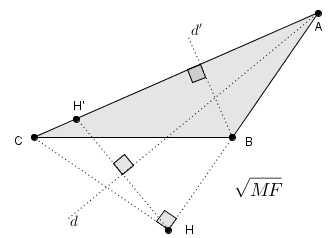
\includegraphics[scale=0.8]{de12.png}
\end{minipage}
\begin{minipage}{0.58\textwidth}
Một bài tập cơ bản minh họa cho phương pháp dựng hình. Các yếu tố cho trước: $d$, $d'$, $H$.\\
Từ đó, ta sẽ "dựng" được $H'$ (tức là tìm được tọa độ) đối xứng với $H$ qua $d$. Do $d$ là đường phân giác trong $\goc{BAC}$ nên $H'\in AC$. Từ đó ta sẽ dựng được đường thẳng $AC$ qua $H'$ vuông góc với $d'$.\\
$A=AC\cap d$, ta dựng được đường thẳng $AH$, $B=AH\cap d'$. Ta cũng dựng được đường thẳng $CH$ qua $H$ vuông góc $AB$ và $C=CH\cap AC$.
\end{minipage}

Với phân tích như thế, ta sẽ tìm được $B\left(0;\frac 13\right)$, $C\left(-\frac{10}3;\frac 34\right)$.

\deda{
Giải hệ phương trình $\hpt{xy(x+1)=x^3+y^2+x-y\quad (1)\\ 3y(2+\sqrt{9x^2+3})+(4y+2)(\sqrt{1+x+x^2}+1)=0\quad (2)}$.
}
\hda 
Với $(1)$, phân tích thành nhân tử ta sẽ được $(x-y)(x^2-y+1)=0\iff  \hoac{y=x\\ y=x^2+1}$.\\
Với $y=x^2+1$ thế vào $(2)$ dễ thấy vô nghiệm.\\
Với $y=x$ thế vào $(2)$ ta được
$$ 3x(2+\sqrt{9x^2+3})+(4x+2)(\sqrt{1+x+x^2}+1)=0$$ 
$$\iff  3x(2+\sqrt{9x^2+3})=(-2x-1)(\sqrt{3+(-2x-1)^2}+2)\iff  f(3x)=f(-2x-1) $$
Với $f(t)=t(\sqrt{t^2+2})$ là một hàm đồng biến nên ta được $3x=-2x-1\iff  x=-\frac 15$.\\
Nghiệm hệ là $\left(-\frac 15;-\frac 15\right)$.
\deda{
Cho $a,b,c>0$ thỏa mãn $a+b+c=2$. Tìm GTLN
$$ S=\sqrt{\dfrac{ab}{ab+2c}}+\sqrt{\dfrac{bc}{bc+2a}}+\sqrt{\dfrac{ca}{ca+2b}}. $$
}
\hda 
Ta có
$$ \sqrt{\frac{ab}{ab+2c}}=\sqrt{\frac{ab}{ab+(a+b+c)c}}=\sqrt{\frac{ab}{(a+c)(b+c)}}\le \frac 12\left(\frac{a}{a+c}+\frac{b}{b+c}\right). $$
Đẳng thức xảy ra khi $\frac{a}{a+c}=\frac{b}{b+c}$. Tương tự ta cũng có 
$$ \sqrt{\frac{bc}{bc+2a}}\le\frac 12\left(\frac b{b+a}+\frac c{c+a}\right);\quad \sqrt{\frac{ca}{ca+2b}}\le\frac 12\left(\frac c{c+b}+\frac{a}{a+b}\right). $$
Cộng các vế ta được $$S\le \frac 12\left(\frac{a+b}{a+b}+\frac{b+c}{b+c}+\frac{c+a}{c+a}\right)=\frac 32.$$
Vậy $S_{\max}=\frac 32$ khi $a=b=c=\frac 23$.
\section{Đề 13}

\deda{
Giải hệ phương trình $\hpt{y^2-x\sqrt{\dfrac{y^2+2}{x}}=2x-2\quad (1)\\ \sqrt{y^2+1}+\sqrt[3]{2x-1}=1\quad (2)}$.
}
\hda 
Đk: $x>0$. Với $(1)$, chia cả hai vế cho $x$ ta được
$$ \dfrac{y^2+2}{x}-\sqrt{\dfrac{y^2+2}x}-2=0\iff  \sqrt{\dfrac{y^2+2}{x}}=2\iff  y^2=4x+2. $$
Thế vào $(2)$ được $\sqrt{4x-1}+\sqrt[3]{2x-1}=1$.\\
Đặt $\sqrt{4x-1}=u\ge 0$; $\sqrt[3]{2x-1}=v$. Ta được $\hpt{u+v=1\\ u^2-2v^3=1}\iff  \hpt{u=1\\ v=0}$.\\
Từ đó ta được nghiệm hệ $\left(\frac 12;0\right)$.
\deda{
 \bd cho $A(2;1)$, $B(-1;-3)$ và hai đường thẳng $d_1$: $x+y+3=0$, $d_2$: $x-5y-16=0$. Tìm tọa độ $C\in d_1$ và $D\in d_2$ sao cho $ABCD$ là hình bình hành.
}
\hda 
Ta có, $C(c;-c-3)\in d_1$, $D(5d+16;d)\in d_2$ nên $\vt{CD}=(5d+16-c;d+c+3)$.\\
Do $ABCD$ là hình bình hành nên $\vt{BA}=\vt{CD}$ từ đó ta tìm được $d=-2$, $c=3$ và $C(3;-6)$, $D(6;-2)$.

\deda{
Cho $x,y\in \mathbb{R}$ thỏa mãn $x^2+y^2+xy=3$. Tìm GTLN và GTNN $P=x^3+y^3-3x-3y$.
}
\hda 
Ta có
$$ P=x^3+y^3-3x-3y=(x+y)^3-3xy(x+y)-3(x+y). $$
Lại có $x^2+y^2+xy=3\iff  xy=(x+y)^2-3$, nên
$$ P=t^3-3(t^2-3)t-3t=-2t^3+6t=f(t). $$
Với $t=x+y$. Mà $t^2-3=xy\le\frac{(x+y)^2}{4}=\frac{t^2}4$, nên $t\in[-2;2]$.\\
Xét $f(t)$ với $t\in[-2;2]$ ta tìm được $P_{\max}=4$, $P_{\min}=-4$.
\section{Đề 14}

\deda{
\bd cho hình vuông $ABCD$. $F\left(\dfrac{11}2;3\right)$ là trung điểm $AD$. $EK$: $19x-8y-18=0$ với $E$ là trung điểm $AB$, $K$ thuộc cạnh $CD$ sap cho $KD=3KC$. Tìm tọa độ $C$ biết $x_E<3$.
}
\hda
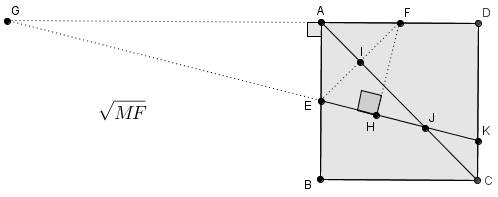
\includegraphics[scale=0.8]{de14.png}\\
Kẻ $FH\bot EK$, $FH=d(F, EK)=\frac{25}{2\sqrt{17}}$.\\
Gọi $G=AD\cap EK$, hình vuông có độ dài cạnh là $a$. Ta tính được $GE=\frac{a\sqrt{17}}2$, $GF=\frac{5a}2$. Hơn nữa, $\frac{AE}{FH}=\frac{GE}{GF}=\frac{\sqrt{17}}5$. Nên ta sẽ tính được $a=5$.\\
Khi đó $EF=\frac{5\sqrt 2}2$, mà $E\in EF$, $x_E<3$ nên ta tìm được $E\left(2;\frac 52\right)$.\\
Gọi $I\left(\frac{15}4;\frac{11}4\right)$ là trung điểm $EF$, suy ra $AC$: $7x+y-29=0$ (qua $I$ vuông góc với $EF$).\\
Gọi $P=AC\cap EF$, ta tìm được $P\left(\frac{10}3;\frac{17}3\right)$, hơn nữa $\vt{IC}=\frac 95\vt{IP}$ nên $C(3;8)$.



\deda{
Giải hệ phương trình $\hpt{|x-2y|+1=\sqrt{x-3y}\\ x(x-4y+1)+y(4y-3)=5}$.
}
\hda 
Đk: $x\ge 3y$. Đặt $|x-2y|=u\ge 0$; $|\sqrt{x-3y}|=v\ge 0$. ta được hệ
$$ \hpt{u-v=-1\\ u^2+v^2=5}\iff  \hpt{u=1\\v=2}. $$
Từ đó giải hệ ta được nghiệm $(-5;-3)$; $(-11;-5)$.
\deda{
Cho $a,b,c>0$. CMR
$$ \dfrac{a^2+1}{4b^2}+\dfrac{b^2+1}{4c^2}+\dfrac{c^2+1}{4a^2}\ge \dfrac{1}{a+b}+\dfrac{1}{b+c}+\dfrac{1}{c+a}. $$
}
\hda 
Ta có
\begin{eqnarray*}
VT&=&\left(\frac{a^2}{4b^2}+\frac 1{4b^2}\right)+\left(\frac{b^2}{4c^2}+\frac{1}{4c^2}\right)+\left(\frac{c^2}{4a^2}+\frac{1}{4a^2}\right)\\ 
&=&\frac{a}{2b^2}+\frac{b}{2c^2}+\frac{c}{2a^2}=\frac 12\left(\frac a{b^2}+\frac b{c^2}+\frac{c}{a^2}\right). 
\end{eqnarray*}
Mà
$$ \frac{a}{b^2}+\frac 1a\ge\frac 2b;\quad \frac{b}{c^2}+\frac 1b\ge \frac 2c;\quad \frac{c}{a^2}+\frac 1c\ge \frac 2a. $$
Nên
$$ \frac{a}{b^2}+\frac{b}{c^2}+\frac{c}{a^2}\ge \frac 1a+\frac 1b+\frac 1c. $$
Suy ra
$$ VT\ge \frac 12\left(\frac 1a+\frac 1b+\frac 1c\right)=\frac 14\left[\left(\frac 1a+\frac 1b\right)+\left(\frac 1b+\frac 1c\right)+\left(\frac 1c+\frac 1a\right)\right]\ge \frac 14\left( \frac 4{a+b}+\frac 4{b+c}+\frac 4{c+a}\right)=VP. $$
Đẳng thức xảy ra khi $a=b=c=1$.
\section{Đề 15}

\deda{
\bd cho hình thang $ABCD$ vuông tại $A,D$; diện tích hình thang bằng $6$; $CD=2AB$, $B(0;4)$. Biết $I(3;-1)$, $K(2;2)$ lần lượt nằm trên đường thẳng $AD$ và $DC$. Viết phương trình đường thẳng $AD$ biết $AD$ không song song với trục tọa độ.
}
\hda 
Vì $AD$ không song song với các trục tọa độ nên gọi VTPT của $AD$ là $\vt{n}=(1,a)$ $(a\neq 0)$.\\
Suy ra $AD$: $x+ay+a-3=0$ và $DC$: $ax-y-2a+2=0$.\\
Từ đó ta tính được $d(B,DC)=\frac{|2a+2|}{\sqrt{a^2+1}}$, $d(B,AD)=\frac{|5a-3|}{\sqrt{a^2+1}}$.\\
Mà $S_{ABCD}=\frac 12AD.(AB+CD)=6$ nên ta sẽ tìm được $a=1$, $a=-\frac 53$, $a=\frac{-1\pm2\sqrt 2}7$.

\deda{
Giải hệ phương trình $\hpt{x+\sqrt{x(x^2-3x+3)}=\sqrt[3]{y+2}+\sqrt{y+3}+1\quad (1)\\ 3\sqrt{x-1}-\sqrt{x^2-6x+6}=\sqrt[3]{y+2}+1\quad (2)}$.
}
\hda 
Đk: $x\in [1;3-\sqrt{3}]\cup [3+\sqrt 3;+\infty)$; $y\in[-3;+\infty)$.\\
$$ (1)\iff  x-1+\sqrt{(x-1)^3+1}=\sqrt[3]{y+2}+\sqrt{(\sqrt[3]{y+2})^3+1}\iff  f(x-1)=f(\sqrt[3]{y+2}). $$
Với $f(t)=t+\sqrt{t^3+1}$, $t\ge -1$  là hàm đồng biến nên ta có $x-1=\sqrt[3]{y+2}$. Thế vào $(2)$ ta được
$$ 3\sqrt{x-1}-\sqrt{x^2-6x+6}=(x-1)+1\iff  (x-1)+1+\sqrt{(x-1)^2-4(x-1)+1}=3\sqrt{x-1}. $$
Do $x=1$ không thỏa mãn nên chia cả hai vế cho $\sqrt{x-1}>0$ ta được
$$ \sqrt{x-1}+\dfrac{1}{\sqrt{x-1}}+\sqrt{x-1-4+\dfrac 1{x-1}}=3\iff  t+\sqrt{t^2-6}=3\iff  t=\dfrac 52. $$
Với $t=\sqrt{x-1}+\dfrac{1}{x-1}>2$. Từ đó ta tìm được nghiệm hệ $(5;62)$, $\left(\frac 54;-\frac{127}{64}\right)$.
\deda{
Cho $x,y>0$ thỏa mãn $x-y+1\le 0$. Tìm GTLN
$$ T=\dfrac{x+3y^2}{\sqrt{x^2+y^4}}-\dfrac{2x+y^2}{5x+5y^2}. $$
}
\hda 
Ta có $x\le y-1\implies  0<\frac x{y^2}\le\frac 1y-\frac 1{y^2}=\frac 14-\left(\frac 1y-\frac 12\right)^2\le \frac 14$. Đặt $t=\frac{x}{y^2}\implies  t\in(0;\frac 14]$.\\
Suy ra
$$ T=\frac{\frac{x}{y^2}+3}{\sqrt{\left(\frac{x}{y^2}\right)^2+1}}-\frac 15\cdot\frac{2\frac{x}{y^2}+1}{\frac{x}{y^2}+1}=\frac{t+3}{\sqrt{t^2+1}}-\frac 15\cdot\frac{2t+1}{t+1}=f(t). $$
$$ f'(t)=\frac{1-3t}{\sqrt{(t^2+1)^3}}-\frac 15\cdot\frac{1}{(t+1)^2}. $$
Do $t\in(0;\frac 14]$ nên $1-3t\ge \frac 14$; $\sqrt{(t^2+1)^3}\le \sqrt{\left(\frac{17}{16}\right)^3}\implies  \frac{1-3t}{\sqrt{(t^2+1)^3}}\ge \frac{4}{17\sqrt{\frac{17}{16}}}$.\\
Và $-\frac 15\cdot\frac{1}{(t+1)^2}>-\frac 15$. Suy ra $f'(t)>0$.\\
Vậy $f(t)$ đồng biến trên $(0;\frac 14]\implies  f(t)\le f(\frac 14)=\frac{13}{\sqrt{17}}-\frac 6{25}$.
\section{Lời giải đề 16}
\deda{Trong mặt phẳng hệ tọa độ $Oxy$, cho đường thẳng $d: x-y+1-\sqrt{2}=0$ và điểm $A(-1;1)$. Viết phương trình đường tròn $(C)$ qua $A$, gốc tọa độ $O$ và tiếp xúc đường thẳng $d$.}
\lgi 
\begin{itemize}[label=, leftmargin=*]
\item Gọi $M$ là trung điểm của $OA$ thì $M\left(-\dfrac{1}{2};\dfrac{1}{2} \right)$
\item Ta có $\vv{OA}=(-1;1)$ là vectơ pháp tuyến của trung trực đoạn $OA$, do đó trung trực đoạn $OA$ có phương trình $x-y+1=0$
\item Tâm $I$ của đường tròn $(C)$ nằm trên trung trực đoạn $OA$ nên suy ra $I(t,t+1)$.
\item Theo đề ta có $IA=d(I,d)\Leftrightarrow \sqrt{(t+1)^2+t^2}=\dfrac{\left|t-t-1+1\sqrt{2} \right|}{\sqrt{2}}\Leftrightarrow 2t^2+2t=0\Leftrightarrow \hay{t=0 \\ t=-1}$ 
\item Khi $t=0$ thì $I(0;1)$ và bán kính $R$ của $(C)$ là 1. Phương trình đường tròn $(C):x^2+(y-1)^2=1$
\item Khi $t=-1$ thì $I(-1;0)$ và bán kính $R$ của $(C)$ là 1. Phương trình đường tròn $(C):(x+1)^2+y^2=1$
\end{itemize}

% câu 9
\deda{Giải hệ phương trình $\va{x^3+y^3+3(y-1)(x-y)=2 \\ \sqrt{x+1}+\sqrt{y+1}=\dfrac{(x-y)^2}{8}}$}
\lgi 
\begin{itemize}[label=,leftmargin=*]
\item Điều kiện: $x,y\ge -1$
\item Phương trình đầu tương đương
\item $\begin{aligned}[t]
&(x+y)^3-8+6-3xy(x+y)+3(y-1)(x-y)=0 \\
\Leftrightarrow \ &(x+y-2)(x^2+y^2+2xy+2x+2y+4)-3(x+y-2)(xy+y+1)=0 \\
\Leftrightarrow \ &(x+y-2)(x^2-xy+y^2+2x-y+1)=0 \\
\Leftrightarrow \ & \hay{x+y-2=0 \\ x^2-xy+y^2+2x-y+1=0 \quad (*)}
 \end{aligned}$
 \item Phương trình $(*)\Leftrightarrow x^2+(2-y)x+y^2-y+1=0$
 \item Phương trình này có $\Delta=-3y^2\le 0$.
 \item Nếu $y \ne 0$ thì $\Delta<0$ dẫn đến hệ phương trình vô nghiệm.
 \item Nếu $y=0$ thì $x=-1$, cũng không thỏa hệ phương trình.
 \item Với $x+y-2=0$, thay $y=2-x$ vào phương trình thứ hai ta được:
 \item $\begin{aligned}[t] 
&2\sqrt{x+1}+2\sqrt{3-x}=x^2-2x+1 \\
\Leftrightarrow \ & (2\sqrt{x+1}-x-1)+(2\sqrt{3-x}+x-3)=x^2-2x-3 \\
\Leftrightarrow \ & (x^2-2x-3)\left(1+\dfrac{1}{2\sqrt{x+1}+x+1}+\dfrac{1}{2\sqrt{3-x}+3-x} \right)=0 \\
\Leftrightarrow \ &x^2-2x-3=0 \\
\Leftrightarrow \ & \hay{x=-1 \\ x=3 }
 \end{aligned}$
 \item Với $x=-1$ thì $y=3$
 \item Với $x=3$ thì $y=-1$
 \item So điều kiện hệ đã cho có nghiệm $(-1;3)$, $(-3;1)$
\end{itemize}


% câu 10
\deda{Giả sử $x$ và $y$ không đồng thời bằng 0. Chứng minh
$$-2\sqrt{2}-2\le \dfrac{x^2-(x-4y)^2}{x^2+4y^2}\le 2\sqrt{2}-2$$}
\lgi 
\begin{itemize}[label=,leftmargin=*]
\item Nếu $y=0$, khi đó $x\ne 0$. Ta có $\dfrac{x^2-(x-4y)^2}{x^2+4y^2}=0$, bất đẳng thức hiển nhiên đúng.
\item Nếu $y\ne 0$ khi đó $\begin{aligned}[t] &-2\sqrt{2}-2 \le \dfrac{x^2-(x-4y)^2}{x^2+4y^2}\le 2\sqrt{2}-2 \\
\Leftrightarrow \ & -2\sqrt{2}-2 \le \dfrac{\left(\frac{x}{2y} \right)^2-\left(\frac{x}{2y}-2\right)^2}{\left(\frac{x}{2y}\right)^2+1}\le 2\sqrt{2}-2 \quad (1)\end{aligned}$
\item Đặt $\dfrac{x}{2y}=\tan t$, khi đó 
\item $\begin{aligned}[t] (1) & \Leftrightarrow -2\sqrt{2}-2 \le \dfrac{\tan ^2t-(\tan t-2)^2}{\tan ^2t+1} \le 2\sqrt{2}-2 \\
&\Leftrightarrow -2\sqrt{2}-2 \le \cos ^2t(4\tan t-4)\le 2\sqrt{2}-2 \\
& \Leftrightarrow -2\sqrt{2}-2\le 2\sin 2t-4\cos ^2t\le 2\sqrt{2}-2 \\
& \Leftrightarrow -\sqrt{2}-1 \le \sin 2t-2\cos ^2t\le \sqrt{2}-1 \\
& \Leftrightarrow -\sqrt{2}\le \sin 2t-\cos 2t\le \sqrt{2} \\
&\Leftrightarrow - \sqrt{2}\le \sqrt{2}\sin \left(2t-\dfrac{\pi}{4} \right)\le 1\\
& \Leftrightarrow -1 \le \sin \left( 2t-\dfrac{\pi}{4}\right) \le \sqrt{2} \end{aligned}$
\item Bất đẳng thức cuối cùng luôn đúng, vậy ta có điều phải chứng minh.
\end{itemize}
\section{Lời giải đề 17}

\deda{Trong mặt phẳng tọa độ $Oxy$, cho tam giác $ABC$ nhọn có đỉnh $A(-1;4)$, trực tâm $H$. Đường thẳng $AH$ cắt cạnh $BC$ tại $M$, đường thẳng $CH$ cắt $AB$ tại $N$. Tâm đường tròn ngoại tiếp tam giác $HMN$ là $I(2;0)$, đường thẳng $BC$ đi qua điểm $P(1;-2)$. Tìm tọa độ các đỉnh $B,C$ của tam giác biết đỉnh $B$ thuộc đường thẳng $x+2y-2=0$.}
\lgi 

\begin{minipage}{12cm}
\begin{itemize}[label=,leftmargin=*]
\item Dễ thấy $BMHN$ là tứ giác nội tiếp. Suy ra $I$ là trung điểm $BH$.
\item $B\in d\Rightarrow B(2-2t;t)$. 
\item Suy ra $H(2+2t;-t)$. 
\item Từ đó $\vv{AH}=(3+2t;-t-4), \vv{BP}=(2t-1;-t-2)$.
\item Do $H$ là trực tâm $\triangle ABC$ nên 
\item $\begin{aligned}[t] \vv{AH}.\vv{BP}=0 &\Leftrightarrow (2t+3)(2t-1)+(t+4)(t+2)=0 \\
& \Leftrightarrow 5t^2+10t+5=0 \\
& \Leftrightarrow t=-1 \end{aligned}$
\end{itemize}
\end{minipage} \begin{minipage}{8cm}
\definecolor{ttttff}{rgb}{0.2,0.2,1.}
\definecolor{qqttcc}{rgb}{0.,0.2,0.8}
\definecolor{ffqqqq}{rgb}{1.,0.,0.}
\begin{tikzpicture}[line cap=round,line join=round,>=triangle 45,x=1.0cm,y=1.0cm]
\clip(0.2,-0.82) rectangle (6.64,4.52);
\draw [color=qqttcc] (3.,4.)-- (1.,0.);
\draw [color=qqttcc] (1.,0.)-- (6.,0.);
\draw [color=qqttcc] (6.,0.)-- (3.,4.);
\draw [color=ttttff] (2.,0.75) circle (1.25cm);
\draw [color=qqttcc] (3.,1.5)-- (1.,0.);
\draw [color=qqttcc] (2.,2.)-- (6.,0.);
\draw [color=qqttcc] (3.,4.)-- (3.,0.);
\begin{scriptsize}
\draw [fill=ffqqqq] (3.,4.) circle (1.0pt);
\draw[color=ffqqqq] (3.14,4.24) node {$A$};
\draw [fill=ffqqqq] (1.,0.) circle (1.0pt);
\draw[color=ffqqqq] (0.76,-0.1) node {$B$};
\draw [fill=ffqqqq] (6.,0.) circle (1.0pt);
\draw[color=ffqqqq] (6.14,-0.2) node {$C$};
\draw [fill=ffqqqq] (3.,1.5) circle (1.0pt);
\draw[color=ffqqqq] (3.14,1.74) node {$H$};
\draw [fill=ffqqqq] (3.,0.) circle (1.0pt);
\draw[color=ffqqqq] (3.12,-0.25) node {$M$};
\draw [fill=ffqqqq] (2.,2.) circle (1.0pt);
\draw[color=ffqqqq] (1.84,2.28) node {$N$};
\draw [fill=ffqqqq] (5.,0.) circle (1.0pt);
\draw[color=ffqqqq] (5.1,-0.24) node {$P$};
\draw [fill=ffqqqq] (2.,0.75) circle (1.0pt);
\draw[color=ffqqqq] (2.1,0.56) node {$I$};
\end{scriptsize}
\end{tikzpicture}
\end{minipage}
\begin{itemize}[leftmargin=*,label=]
\item Từ đó $H(0;1),B(4;-1),\vv{AH}=(1;-3)$. Đường thẳng $BC:x-3y-7=0$
\item Đường thẳng $AC:2x-y+6=0$. Từ đó tọa độ $C(-5;-4)$.
\end{itemize}

% cau 9
\deda{Giải hệ phương trình:
$ \va{
\dfrac{2}{(\sqrt{x}+\sqrt{y})^2}+\dfrac{1}{x+\sqrt{y(2x-y)}}=\dfrac{2}{y+\sqrt{x(2x-y)}}
\\

2(y-4)\sqrt{2x-y-3}-(x-6)\sqrt{x+y+1}=3(y-2)
 }$}
\lgi 
\begin{itemize}[leftmargin=*,label=]
\item Điều kiện: $\va{x\ge 0, y \ge 0 \\ 2x-y\ge 0 \\ 2y-x \ge 0 \\ 2x-y-3\ge 0}$
\item Nếu $y=0$ thi phương trình đầu trở thành $\dfrac{2}{x}+\dfrac{1}{x}=\dfrac{2}{\sqrt{2x^2}}\Leftrightarrow \dfrac{3}{x}=\dfrac{\sqrt{2}}{x}$. Dẫn đến hệ vô nghiệm.
\item Tương tự $x=0$ cũng không là nghiệm của hệ. 
\item Xét $x,y>0$. Đặt $t=\dfrac{x}{y}$, thế thì $t>0$. Phương trình đầu trở thành
\item $\begin{aligned}[t] 
\dfrac{2}{(\sqrt{t}+1)^2}+\dfrac{1}{t+\sqrt{2t-1}}=\dfrac{2}{1+\sqrt{t(2t-1)}} &\Leftrightarrow \dfrac{2}{(\sqrt{t}+1)^2}+\dfrac{2}{2t-1+2\sqrt{2t-1}+1}=\dfrac{2}{1+\sqrt{t(2t-1)}}\\
&\Leftrightarrow \dfrac{2}{(\sqrt{t}+1)^2}+\dfrac{2}{(\sqrt{2t-1}+1)^2}=\dfrac{2}{1+\sqrt{t(2t-1)}} (1)
\end{aligned}$
\item Đặt $\va{a=\sqrt{t}\\ b=\sqrt{2t-1}} (a,b>0)$. Khi đó $(1)\Leftrightarrow \dfrac{1}{(1+a)^2}+\dfrac{1}{(1+b)^2}=\dfrac{1}{1+ab}$
\item Ta sẽ chứng minh bổ đề sau: $\dfrac{1}{(1+a)^2}+\dfrac{1}{(1+b)^2}\ge \dfrac{1}{1+ab}$ $\forall a,b>0$
\item Theo BĐT Cauchy-Schwarz ta có 
\item $(1+ab)(a+b)\ge (\sqrt{a}+\sqrt{ab}.\sqrt{b})^2=a(1+b)^2\Rightarrow \dfrac{1}{(1+b)^2}\ge \dfrac{a}{a+b}.\dfrac{1}{1+ab}$
\item Tương tự $\dfrac{1}{(1+a)^2}\ge \dfrac{b}{a+b}.\dfrac{1}{1+ab}$
\item Cộng 2 BĐT vế theo vế ta được $\dfrac{1}{(1+a)^2}+\dfrac{1}{(1+b)^2} \ge \dfrac{a+b}{a+b}.\dfrac{1}{1+ab}=\dfrac{1}{1+ab}$
\item Bổ đề được chứng minh. Đẳng thức xảy ra khi $a=b$. Tức $\sqrt{t}=\sqrt{2t-1}\Leftrightarrow t=1\Leftrightarrow x=y$
\item Thay $y=x$ vào phương trình thứ hai ta được $2(x-4)\sqrt{x-3}-(x-6)\sqrt{2x+1}=3(x-2)$ (2)
\end{itemize}


\deda{Cho ba số thực $a,b,c$ thỏa mãn $a>2,b>0,c>0$. Tìm giá trị lớn nhất của biểu thức:
$$P=\dfrac{1}{2\sqrt{a^2+b^2+c^2-4a+5}}-\dfrac{1}{(a-1)(b+1)(c+1)}$$}
\lgi 
\begin{itemize}[label=,leftmargin=*]
\item Đặt $a_1=a-2$, thế thì $a_1>0$. Khi đó $P=\dfrac{1}{2\sqrt{a_1^2+b^2+c^2+1}}-\dfrac{1}{(a_1+1)(b+1)(c+1)}$
\item Ta có $a_1^2+b^2+c^2+1 \ge \dfrac{(a_1+b)^2}{2}+\dfrac{(c+1)^2}{2}\ge \dfrac{1}{4}(a_1+b+c+1)^2$
\item Ta lại có $(a_1+1)(b+1)(c+1)\le \left(\dfrac{a_1+1+b+1+c+1}{3} \right)^3=\left(\dfrac{a_1+b+c+3}{3} \right)^3$
\item Do đó $P\le \dfrac{1}{a_1+b+c+1}-\dfrac{27}{(a_1+b+c+3)^3}$.
\item Đặt $t=a_1+b+c$, khi đó $t>1$. Khi đó $P\le \dfrac{1}{t}-\dfrac{27}{(t+2)^3}$
\item Xét hàm số $f(t)=\dfrac{1}{t}-\dfrac{27}{(t+2)^3}$ trên miền $(1;+\infty)$
\item $f'(t)=-\dfrac{1}{t^2}+\dfrac{81}{(t+2)^4}$. Khi đó $f'(t)=0 \Leftrightarrow (t+2)^4=81t^2\Leftrightarrow t=4$ (do $t>1$)
\item Lập bảng biến thiên:
\item 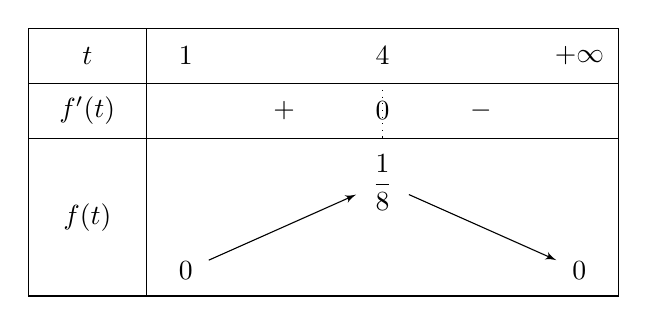
\begin{tikzpicture}
\tkzTabInit[lgt=1.5,espcl=2.5,deltacl=.5]
{$t$ /.7, $f'(t)$ /.7,$f(t)$ /2}
{1, $4$ , $+\infty$}
\tkzTabLine{,+,z,-,}
\tkzTabVar{-/0 ,+/ $\dfrac{1}{8}$ ,-/0}
\end{tikzpicture}
\item Từ bảng biến thiên ta có $f(t)\le f(4)=\dfrac{1}{8} \ \forall t > 1$. Vậy $P\le \dfrac{1}{8}$.
\item Đẳng thức xảy ra khi $a=3,b=c=1$. Vậy $\max P=\dfrac{1}{8}$
\end{itemize}

\section{Lời giải đề 18}
\deda{Trong mặt phẳng với hệ trục tọa độ $Oxy$. Viết phương trình các cạnh của hình vuông $ABCD$, biết rằng các đường thẳng $AB,CD,BC,AD$ lần lượt đi qua các điểm $M(2;4),N(2;-4),P(2;2),Q(3;-7)$.}
\lgi 
\begin{itemize}[label=,leftmargin=*]
\item Gọi $\vv{n}=(a,b)$ là vectơ pháp tuyến của đường thẳng $AB$. Vì $AB$ đi qua điểm $M(2;4)$ nên phương trình tổng quát của $AB$ là $ax+by-2a-4b=0$. 
\item Đường thẳng $BC$ đi qua $P(2;2)$ và vuông góc với $AB$ nên có phương trình $-bx+ay-2a+2b=0$ 
\item $ABCD$ là hình vuông nên $d(N,AB)=d(Q,BC)$.
\item Hay $\dfrac{|2a-4b-2a-4b|}{\sqrt{a^2+b^2}}=\dfrac{|-3b-7a-2a+2b|}{\sqrt{a^2+b^2}}\Leftrightarrow \hay{9a=-9b \\ 9a=7b}$
\item Với $9a=-9b$, chọn $a=1\Rightarrow b=-1$
\item Phương trình $AB:x-y+2=0$, phương trình $BC:x+y-4=0$
\item Đường thẳng $CD$ đi qua $N(2;-4)$ và song song với $AB$ nên có phương trình $x-y-6=0$
\item Đường thẳng $AD$ đi qua $Q(3;-7)$ và song song với $BC$ nên có phương trình $x+y+4=0$
\item Với $9a=7b$, chọn $a=7,b=9$.
\item Phương trình $AB:7x+9y-50=0$, phương trình $BC:-9x+7y+4=0$.
\item Phương trình $CD:7x+9y+22=0$, phương trình $AD:-9x+7y+76=0$
\end{itemize}

\deda{Giải hệ phương trình:
$ \va{2x^2-y^2-7x+2y+6=0
 \\
 -7x^3+12x^2y-6xy^2+y^3-2x+2y=0 }
(x,y \in \mathbb{R}) $.}
\lgi 
 Ta có $-7x^3+12x^2y-6xy^2+y^3-2x+2y=0\Leftrightarrow (x-y)\left[x^2-x(y-2x)+(y-2x)^2+2 \right]=0 \ (*)$ \\
 Vì $x^2-x(y-2x)+(y-2x)^2+2=\left[y-2x-\dfrac{x}{2} \right]^2+\dfrac{3x^2}{4}+2 >0 \ \forall x,y$ nên $(*)\Leftrightarrow x=y$\\
 Thay $y=x$ vào phương trình sau ta được $x^2-5x+6=0 \Leftrightarrow \hay{x=2\\ x=3}$\\
 Vậy hệ có nghiệm $(x,y)=(2;2)$, $(x,y)=(3;3)$
 
\deda{Cho các số thực không âm $a,b,c$ thỏa mãn $a^2+b^2+c^2-3b \le 0$. Tìm giá trị nhỏ nhất của biểu thức
$$P=\dfrac{1}{(a+1)^2}+\dfrac{4}{(b+2)^2}+\dfrac{8}{(c+3)^2}$$}
\lgi 
 Ta có $a^2+b^2+c^2-2a-4b-2c+6=(a-1)^2+(b-2)^2+(c-1)^2 \ge 0$, theo giả thiết thì $a^2+b^2+c^2 \le 3b$.\\
 Suy ra $3b-2a-4b-2c+6 \le 0 \Leftrightarrow 2a+b+2c\le 6\Leftrightarrow 2a+b+2c+10\le 16$\\
 Với hai số $x,y>0$ thì $\dfrac{1}{x^2}+\dfrac{1}{y^2}\ge \dfrac{8}{(x+y)^2}$.
 Áp dụng nhận xét trên ta có\\
 $P=\dfrac{1}{(a+1)^2}+\dfrac{4}{(b+2)^2}+\dfrac{8}{(c+3)^2}\ge \dfrac{8}{\left(a+\frac{b}{2}+2 \right)^2}+\dfrac{8}{(c+3)^2}\ge \dfrac{8.8}{\left(a+\frac{b}{2}+c+5 \right)^2}=\dfrac{16^2}{(2a+b+2c+10)^2}\ge 1$\\
 Đẳng thức xảy ra khi $a=c=1, b=2$. Vậy $\min P=1$.



\section{Lời giải đề 19}
\deda{Trong mặt phẳng với hệ trục tọa độ $Oxy$, cho hình vuông $ABCD$. Điểm $N(1;-2)$ thỏa mãn $2\vv{NB}+\vv{NC}=\vv{0}$ và điểm $M(3;6)$ thuộc đường thẳng chứa cạnh $AD$. Gọi $H$ là chân hình chiếu vuông góc của $A$ xuông đường thẳng $DN$. Xác định tọa độ của các đỉnh của hình vuông $ABCD$ biết khoảng cách từ điểm $H$ đến cạnh $CD$ bằng $\dfrac{12\sqrt{2}}{13}$ và đỉnh $A$ có hoành độ là một số nguyên lớn hơn -2.}
\lgi 
\begin{minipage}{12cm}
\begin{itemize}[leftmargin=*,label=]
\item Gọi $E$ là hình chiếu vuông góc của $H$ trên $CD\Rightarrow HE=\dfrac{12\sqrt{2}}{13}$
\item Giả sử cạnh hình vuông là $a$ ($a>0$)
\item Ta có $2\vv{NB}+\vv{NC}=\vv{0}\Leftrightarrow \vv{CN}=\dfrac{2}{3}\vv{CB}$ nên $N$ nằm giữa $B,C$ và thỏa mãn $NC=\dfrac{2}{3}BC=\dfrac{2a}{3}$.
\item Suy ra $DN=\sqrt{CD^2+CN^2}=\dfrac{a\sqrt{13}}{3}$
\end{itemize}
\end{minipage} \begin{minipage}{6cm}
\definecolor{qqttcc}{rgb}{0.,0.2,0.8}
\definecolor{ffqqqq}{rgb}{1.,0.,0.}
\begin{tikzpicture}[line cap=round,line join=round,>=triangle 45,x=1.5cm,y=1.5cm]
\clip(1.7,-0.58) rectangle (5.54,3.52);
\draw [color=qqttcc] (2.,3.)-- (2.,0.);
\draw [color=qqttcc] (2.,0.)-- (5.,0.);
\draw [color=qqttcc] (5.,0.)-- (5.,3.);
\draw [color=qqttcc] (5.,3.)-- (2.,3.);
\draw [color=qqttcc] (5.,3.)-- (3.,0.);
\draw [color=qqttcc] (2.,3.)-- (4.076923076923077,1.6153846153846154);
\draw [color=qqttcc] (4.076923076923077,1.6153846153846154)-- (5.,1.6153846153846154);
\begin{scriptsize}
\draw [fill=ffqqqq] (2.,3.) circle (1.0pt);
\draw[color=ffqqqq] (2.14,3.24) node {$A$};
\draw [fill=ffqqqq] (2.,0.) circle (1.0pt);
\draw[color=ffqqqq] (2.04,-0.24) node {$B$};
\draw [fill=ffqqqq] (5.,0.) circle (1.0pt);
\draw[color=ffqqqq] (5.12,-0.2) node {$C$};
\draw [fill=ffqqqq] (5.,3.) circle (1.0pt);
\draw[color=ffqqqq] (5.22,3.24) node {$D$};
\draw [fill=ffqqqq] (3.,0.) circle (1.0pt);
\draw[color=ffqqqq] (3.12,-0.2) node {$N$};
\draw [fill=ffqqqq] (4.076923076923077,1.6153846153846154) circle (1.0pt);
\draw[color=ffqqqq] (3.96,1.98) node {$H$};
\draw [fill=ffqqqq] (5.,1.6153846153846154) circle (1.0pt);
\draw[color=ffqqqq] (5.26,1.74) node {$E$};
\end{scriptsize}
\end{tikzpicture}
\end{minipage}
\begin{itemize}[leftmargin=*,label=]
\item Ta có $\triangle ADH\backsim \triangle DNC$ (g.g) nên $\dfrac{AD}{DN}=\dfrac{DH}{NC}\Rightarrow DH=\dfrac{2a}{\sqrt{13}}$
\item $\triangle DHE\backsim DNC$ (g.g) nên $\dfrac{HE}{NC}=\dfrac{DH}{DN}\Rightarrow NC=\dfrac{13}{6}.HE=2\sqrt{2}$
\item Dẫn đến $\dfrac{2a}{3}=2\sqrt{2}\Rightarrow a=3\sqrt{2}$
\item Giả sử vtpt của $AD$ là $\vv{n}=(a;b)$ với $a^2+b^2>0$. Phương trình $AD:ax+by-3a-6b=0$.
\item $d(N,AD)=3\sqrt{2}\Leftrightarrow \dfrac{|-2a-8b|}{\sqrt{a^2+b^2}}=3\sqrt{2}\Leftrightarrow 7a^2-16ab-23b^2=0 \Leftrightarrow (a+b)(7a-23b)=0 \Leftrightarrow \hay{a=-b \\ 7a=23b}$
\item Trường hợp $a=-b$. Chọn $a=1, b=-1$. Phương trình $AD:x-y+3=0$.  
\item Kẻ $NP\perp AD$ ($P\in AD$), khi đó $NP:x+y+1=0 \Rightarrow P(-2;1)$
\item $AP=BN=\dfrac{BC}{3}=\sqrt{2}$. Lại do $A\in AD\Rightarrow A(t;t+3)$ ($t>-2$). Từ $AP=\sqrt{2}$ suy ra $t=-1 (n) \vee t=-3 (\ell)$
\item Với $t=-1$ thì $A(-1;2)$. Khi đó do $\vv{PD}=2\vv{AP}$ nên $D(-4;-1)$. Từ đó tìm được $B(2;-1),C(-1;-4)$
\item Trường hợp $7a=23b$. Giải tương tự ta được 2 giá trị hoành độ $A$ không phải số nguyên. Vậy ta loại trường hợp này.
\item Kết luận $A(-1;2),B(2;-1),C(-1;-4),D(-4;-1)$
\end{itemize}

\deda{Giải hệ phương trình $\va{\sqrt{x^2-x-y-1}.\sqrt[3]{x-y-1}=y+1\\ x+y+1+\sqrt{2x+y}=\sqrt{5x^2+3y^2+3x+7y}}(x,y \in \mathbb{R})$}
\lgi 
\begin{itemize}[label=,leftmargin=*]
\item Điều kiện: $\va{x^2-x-y-1\ge 0 \\ 2x+y \ge 0 \\ 5x^2+3y^2+3x+7y\ge 0}$
\item Nếu $x^2=x+y+1$, từ phương trình đầu suy ra $y+1=0\Rightarrow y=-1\Rightarrow x^2-x=0 \Rightarrow \hay{x=0\\ x=1}$
\item Thử vào phương trình sau thấy $(x,y)=(1;-1)$ thỏa mãn. Suy ra $(1;-1)$ là nghiệm của hệ phương trình.
\item Nếu $x^2>x+y+1$. Phương trình đầu tương đương
\item $\begin{aligned}[t]&\sqrt[3]{x-y-1}=\dfrac{y+1}{\sqrt{x^2-x-y-1}}\\ 
\Leftrightarrow &\sqrt[3]{x-y-1}-1=\dfrac{y+1}{\sqrt{x^2-x-y-1}}-1 \\
\Leftrightarrow &\dfrac{x-y-2}{\sqrt[3]{(x-y-1)^2}+\sqrt[3]{x-y-1}+1} = \dfrac{-(x+y+1)(x-y-2)}{\sqrt{x^2-x-y-1}.(y+1+\sqrt{x^2-x-y-1})} \\
\Leftrightarrow &(x-y-2)\left[\dfrac{1}{\sqrt[3]{(x-y-1)^2}+\sqrt[3]{x-y-1}+1}+\dfrac{x+y+1}{\sqrt{x^2-x-y-1}(\sqrt{x^2-x-y-1}+y+1)}\right]=0\\
\Leftrightarrow &\hay{x-y-2=0 \quad (1) \\ \dfrac{1}{\sqrt[3]{(x-y-1)^2}+\sqrt[3]{x-y-1}+1}+\dfrac{x+y+1}{\sqrt{x^2-x-y-1}(\sqrt{x^2-x-y-1}+y+1)}=0 \quad (*)}\\
 \end{aligned}$
\item Từ điều kiện $\va{2x+y\ge 0 \\ x^2-x-y-1 \ge 0}\Rightarrow x^2+x-1\ge 0\Rightarrow \hay{x>\dfrac{-1+\sqrt{5}}{2} \\ x<\dfrac{-1-\sqrt{5}}{2}}$
\item Nếu $x<\dfrac{-1-\sqrt{5}}{2}$, khi đó từ $2x+y\ge 0 \Rightarrow y \ge -2x\ge 1+\sqrt{5}\Rightarrow x+y+1 >0$, do đó $(*)$ vô nghiệm.
\item Trường hợp $x>\dfrac{-1+\sqrt{5}}{2} \Rightarrow x>0$. Giả sử $y+1 \le 0 \Rightarrow x-(y+1)>0 \Rightarrow VT(1) >0 \ge VP(1)$, dẫn đến hệ vô nghiệm. Suy ra $y+1>0$, từ đây thì pt $(*)$ vô nghiệm.
\item Suy ra $y=x-2$. Thay vào phương trình sau ta được 
\item $2x-1+\sqrt{3x-2}=\sqrt{8x^2-2x-2}\Leftrightarrow 2x-1+\sqrt{3x-2}=\sqrt{2(2x-1)^2+2(3x-2)}$
\item Điều kiện: $x\ge \dfrac{2}{3}$
\item Đặt $\va{a=2x-1 \ (a>\frac{1}{3})\\ b=\sqrt{3x-2} \ (b \ge 0)}$
\item Phương trình trở thành $a+b=\sqrt{2a^2+2b^2}\Leftrightarrow a^2+2ab+b^2=2a^2+2b^2\Leftrightarrow (a-b)^2=0 \Leftrightarrow a=b$
\item Từ đó $2x-1=\sqrt{3x-2}\Leftrightarrow 4x^2-4x+1=3x-2\Leftrightarrow 4x^2-7x+3=0 \Leftrightarrow \hay{x=1 \\ x=\frac{3}{4}}$
\item Với $x=1 \Rightarrow y=-1$, thử lại thấy thỏa mãn. Ta nhận nghiệm $(x;y)=(1;-1)$
\item Với $x=\frac{3}{4}\Rightarrow y=-\frac{5}{4}$. Thử lại không thỏa.
\end{itemize}

\deda{Cho ba số thực không âm $x,y,z$. Tìm giá trị lớn nhất của biểu thức
$$P=\dfrac{4}{\sqrt{x^2+y^2+z^2+4}}-\dfrac{4}{(x+y)\sqrt{(x+2z)(y+2z)}}-\dfrac{5}{(y+z)\sqrt{(y+2x)(z+2x)}}$$}
\lgi 
\begin{itemize}[label=,leftmargin=*]
\item Sử dụng BĐT Cauchy ta có 
\item $\begin{aligned}[t](x+y)\sqrt{(x+2z)(y+2z)	}\le (x+y).\dfrac{x+y+4z}{2}&=\dfrac{x^2+y^2+2xy+4xz+4yz}{2}\\
& \le \dfrac{x^2+y^2}{2}+\dfrac{x^2+y^2}{2}+(x^2+z^2)+(y^2+z^2) \\
&\le 2(x^2+y^2+z^2) \end{aligned}$
\item $(y+z)\sqrt{(y+2x)(z+2x)}\le (y+z).\dfrac{y+z+4x}{2}=\dfrac{y^2+z^2+2yz+4yx+4zx}{2}\le 2(x^2+y^2+z^2)$
\item Khi đó biểu thức $P$ trở thành
\item $P\le \dfrac{4}{\sqrt{x^2+y^2+z^2+4}}-\dfrac{4}{2(x^2+y^2+z^2)}-\dfrac{5}{2(x^2+y^2+z^2)}=\dfrac{4}{\sqrt{x^2+y^2+z^2+4}}-\dfrac{9}{2(x^2+y^2+z^2)}$
\item Đặt $t=\sqrt{x^2+y^2+z^2+4}$, khi đó $t>2$. Khi đó $P \le \dfrac{4}{t}-\dfrac{9}{2(t^2-4)}$
\item Xét hàm số $y=f(t)=\dfrac{4}{t}-\dfrac{9}{2(t^2-4)}$ trên miền $(2;+\infty)$
\item $f'(t)=-\dfrac{4}{t^2}+\dfrac{9t}{(t^2-4)^2}=\dfrac{(4-t)(4t^3+7t^2-4t-16)}{t^2(t^2-4)^2}$
\item Do $t>2$ nên $4t^3+7t^2-4t-16\ge 4(t^3-4)+t(7t-4)>0$, vậy $f'(t)=0\Leftrightarrow t=4$
\item Lập bảng biến thiên ta thu được $f(t) \le f(4)=\dfrac{5}{8}$. Vậy $P\le \dfrac{5}{8}$
\item Đẳng thức xảy ra khi $x=y=z=2$. Vậy $\max P=\dfrac{5}{8}$
\end{itemize}

\section{Lời giải đề 20}
\deda{Trong mặt phẳng $Oxy$, cho hình chữ nhật $ABCD$ có $AB=2BC$. Gọi $H$ là hình chiếu của $A$ lên đường thẳng $BD$. $E,F$ lần lượt là trung điểm cạnh $CD$ và $BH$. Biết $A(1;1)$, phương trình đường thẳng $EF$ là $3x-y-10=0$ và điểm $E$ có tung độ âm. Tìm tọa độ các đỉnh $B,C,D$.}
\lgi 
\begin{minipage}{12cm}
\begin{itemize}[label=,leftmargin=*]
\item Gọi $E,F,G$ lần lượt là trung điểm các đoạn thẳng $CD, BH, AB$. Ta chứng minh $AF\perp EF$.
\item Ta thấy các tứ giác $ADEG$ và $ADFG$ nội tiếp đường tròn đường kính $DG$ nên tứ giác $ADEF$ cũng nội tiếp đường tròn này, do đó $AF\perp EF$.
\item Đường thẳng $AF$ có phương trình $x+3y-4=0$
\end{itemize}
\end{minipage} \begin{minipage}{6cm}
\definecolor{qqttcc}{rgb}{0.,0.2,0.8}
\definecolor{ffqqqq}{rgb}{1.,0.,0.}
\begin{tikzpicture}[line cap=round,line join=round,>=triangle 45,x=1.25cm,y=1.25cm]
\clip(1.74,0.44) rectangle (6.42,3.5);
\draw [color=qqttcc] (2.,3.)-- (6.,3.);
\draw [color=qqttcc] (6.,3.)-- (6.,1.);
\draw [color=qqttcc] (6.,1.)-- (2.,1.);
\draw [color=qqttcc] (2.,1.)-- (2.,3.);
\draw [color=qqttcc] (6.,3.)-- (2.,1.);
\draw [color=qqttcc] (4.,3.)-- (4.,1.);
\draw [color=qqttcc] (4.4,2.2)-- (4.,1.);
\draw [color=qqttcc] (2.,3.)-- (4.,1.);
\draw [color=qqttcc] (2.,3.)-- (2.8,1.4);
\draw [color=qqttcc] (4.,3.)-- (4.4,2.2);
\draw [color=qqttcc] (2.,3.)-- (4.4,2.2);
\begin{scriptsize}
\draw [fill=ffqqqq] (2.,3.) circle (1.0pt);
\draw[color=ffqqqq] (2.14,3.24) node {$A$};
\draw [fill=ffqqqq] (6.,3.) circle (1.0pt);
\draw[color=ffqqqq] (6.14,3.24) node {$B$};
\draw [fill=ffqqqq] (6.,1.) circle (1.0pt);
\draw[color=ffqqqq] (6.02,0.84) node {$C$};
\draw [fill=ffqqqq] (2.,1.) circle (1.0pt);
\draw[color=ffqqqq] (1.94,0.8) node {$D$};
\draw [fill=ffqqqq] (4.,3.) circle (1.0pt);
\draw[color=ffqqqq] (4.14,3.24) node {$G$};
\draw [fill=ffqqqq] (4.,1.) circle (1.0pt);
\draw[color=ffqqqq] (4.,0.8) node {$E$};
\draw [fill=ffqqqq] (4.4,2.2) circle (1.0pt);
\draw[color=ffqqqq] (4.6,2.12) node {$F$};
\draw [fill=ffqqqq] (2.8,1.4) circle (1.0pt);
\draw[color=ffqqqq] (2.48,1.56) node {$H$};
\end{scriptsize}
\end{tikzpicture}
\end{minipage}
\begin{itemize}[label=,leftmargin=*]
\item Tọa độ điểm $F$ là nghiệm của hệ $\va{3x-y=10 \\ x+3y=4} \Leftrightarrow \va{x=\frac{17}{5} \\ y=\frac{1}{5}}\Rightarrow F\left(\dfrac{17}{5};\dfrac{1}{5} \right)\Rightarrow AF=\sqrt{\dfrac{32}{5}}$
\item $\triangle AFE\backsim \triangle DCB\Rightarrow EF=\dfrac{AF}{2}=2\sqrt{\dfrac{2}{5}}$
\item $E\in EF:3x-y-10=0\Rightarrow E(t;3t-10)\Rightarrow \vv{EF}=\left(t-\dfrac{17}{5};3t-\dfrac{51}{5} \right)$.
\item $EF^2=\left(t-\dfrac{17}{5} \right)^2+\left(3t-\dfrac{51}{5} \right)^2=\dfrac{8}{5}\Leftrightarrow 5t^2-34t+57=0\Leftrightarrow t=3 \vee t=\dfrac{19}{5}$
\item $t=3\Rightarrow E(3;-1)$. Với $t=\dfrac{19}{5}$ thì $E\left(\dfrac{19}{5};\dfrac{7}{5} \right)$. Vì $E$ có tung độ âm nên $E(3;-1)$.
\item Phương trình $AE:x+y-2=0$. Vì $\triangle ADE$ vuông cân tại $D$ nên
\item $\va{AD=DE\\ AD\perp DE}\Rightarrow \va{(x-1)^2+(y-1)^2=(x-3)^2+(y+1)^2 \\ (x-1)(x-3)=(y-1)(y+1)}\Leftrightarrow \va{y=x-2 \\ (x-1)(x-3)=0}\Leftrightarrow \va{x=1 \\ y=-1}\vee \va{x=3 \\ y=1}$
\item Với $x=1;y=-1$ thì $D(1;-1)$. Với $x=3;y=1$ thì $D(3;1)$.
\item Do $D$ và $F$ nằm về hai phía so với $AE$ nên $D(1;-1)$
\item Khi đó $C(5;-1),B(1;5)$.
\end{itemize}

\deda{Giải hệ phương trình $\va{2\sqrt{x+y+6}=1-y \\ 9\sqrt{1+x}+xy\sqrt{9+y^2}=0} (x,y\in \mathbb{R})$}
\lgi 
\begin{itemize}[label=,leftmargin=*]
\item Điều kiện $\va{x+y+6 \ge 0 \\ x\ge -1}$
\item Nếu $y\ge 0$, để hệ có nghiệm thì $1\ge y\ge 0$.
\item Khi đó $2\sqrt{x+y+6}\ge 2\sqrt{-1+0+6}=2\sqrt{5}$ mà $1-y\le 1$. Dẫn đến phương trình đầu vô nghiệm.
\item Vậy $y<0$, để phương trình sau có nghiệm thì $x>0$. Ta có 
\item $9\sqrt{1+x}+xy\sqrt{9+y^2}=0 \Leftrightarrow \left(\dfrac{3}{\sqrt{x}} \right)\sqrt{9+\left(\dfrac{3}{\sqrt{x}} \right)^2}=(-y)\sqrt{9+(-y)^2}$ (1)
\item Xét hàm số $f(t)=t\sqrt{9+t^2}$ với $t>0$
\item $f'(t)=\dfrac{9+2t^2}{\sqrt{9+t^2}}>0 \ \forall t>0$. Vậy $f(t)$ đồng biến trên miền $(0;+\infty)$
\item Do đó $(1)\Leftrightarrow \dfrac{3}{\sqrt{x}}=-y\Leftrightarrow x=\dfrac{9}{y^2}$. Thế vào phương trình sau ta được $2\sqrt{\dfrac{9}{y^2}+y+6}=1-y \ (*)$
\item Hàm số $g(y)=2\sqrt{\dfrac{9}{y^2}+y+6}$ đồng biến trên $(-\infty;0)$, hàm số $h(y)=1-y$ nghịch biến trên $(-\infty;0)$ nên phương trình $(*)$ nếu có nghiệm thì đó là nghiệm duy nhất. 
\item Nhận thấy $y=-3$ là nghiệm của $(*)$, vậy $y=-3$ là nghiệm duy nhất của $(*)$.
\item Vậy hệ có nghiệm duy nhất $(x,y)=(1;-3)$.
\end{itemize}

\deda{Cho các số thực dương $ab\ge 1$ và $c(a+b+c)\ge 3$. Tìm giá trị nhỏ nhất của biểu thức 
$$P=\dfrac{b+2c}{1+a}+\dfrac{a+2c}{1+b}+6\ln (a+b+2c)$$}
\lgi 
\begin{itemize}[leftmargin=*,label=]
\item $P+2=\dfrac{a+b+2c+1}{1+a}+\dfrac{a+b+2c+1}{1+b}+6\ln (a+b+2c)=(a+b+2c+1)\left(\dfrac{1}{1+a}+\dfrac{1}{1+b} \right)+6\ln(a+b+2c)$
\item Ta chứng minh bổ đề quen thuộc sau $\dfrac{1}{1+a}+\dfrac{1}{1+b}\ge \dfrac{2}{1+\sqrt{ab}}$ với $ab\ge 1$
\item Thật vậy $\dfrac{1}{1+a}+\dfrac{1}{1+b}\ge \dfrac{2}{1+\sqrt{ab}}\Leftrightarrow (\sqrt{a}-\sqrt{b})^2(\sqrt{ab}-1)\ge 0$ (luôn đúng do $ab \ge 1$)
\item Lại theo BĐT Cauchy: $\sqrt{ab}\le \dfrac{ab+1}{2}$ nên 
\item $\dfrac{2}{1+\sqrt{ab}}\ge \dfrac{4}{3+ab}\ge \dfrac{4}{c^2+ab+bc+ca}=\dfrac{4}{(a+c)(b+c)}\ge \dfrac{16}{(a+b+2c)^2}$
\item Từ đó $P+2\ge \dfrac{16(a+b+2c+1)}{(a+b+2c)^2}+6\ln (a+b+2c)$
\item Đặt $t=	a+b+2c$, thế thì $t>0$. Khi đó $P+2\ge \dfrac{16(t+1)}{t^2}+6\ln t$.
\item Xét hàm $f(t)=\dfrac{16(t+1)}{t^2}+6\ln t$ với $t>0$.
\item $f'(t)=\dfrac{16t^2	-32t(t+1)}{t^4}+\dfrac{6}{t}=\dfrac{-16t-32}{t^3}+\dfrac{6}{t}=\dfrac{6t^2-16t-32}{t^3}$. Khi đó $f'(t)=0 \Leftrightarrow t=4$ (do $t>0$)
\item Lập bảng biến thiên ta được $f(t)\ge f(4)=5+6\ln 4$
\item Vậy $P \ge 3+6\ln 4$. Đẳng thức xảy ra khi $a=b=c=1$. 
\item Kết luận: $\max P=3+6\ln 4$.
\end{itemize}

\section{Lời giải đề 21} 

\deda{Trong mặt phẳng hệ tọa độ $Oxy$ cho tam giác $ABC$ có $A(1;4)$, tiếp tuyến tại $A$ của đường tròn ngoại tiếp tam giác $ABC$ cắt $BC$ tại $D$, đường phân giác trong của $\angle ADB$ có phương trình $x-y+2=0$. Điểm $M(-4;1)$ thuộc cạnh $AC$. Viết phương trình đường thẳng $AB$.}
\lgi 
\begin{minipage}{9cm}
\begin{itemize}[label=,leftmargin=*]
\item Gọi $AI$ là phân giác trong $\angle BAC$.
\item Ta có $\va{\angle AID=\angle ABD+\angle BAI \\ \angle IAD=\angle CAD+\angle IAC}$
\item Mà $\angle BAI=\angle IAC$ và $\angle ABC=\angle CAD$
\item Nên $\angle AID=\angle IAD$. Tức $\triangle AID$ cân tại $D$.
\item Gọi $E$ là giao điểm của phân giác trong $\angle ADB$ với $AB$. Khi đó $DE\perp AI$.
\item Suy ra đường thẳng $AI:x+y-5=0$
\end{itemize}
\end{minipage} \begin{minipage}{9cm}
\definecolor{ttttff}{rgb}{0.2,0.2,1.}
\definecolor{qqttcc}{rgb}{0.,0.2,0.8}
\definecolor{ffqqqq}{rgb}{1.,0.,0.}
\begin{tikzpicture}[line cap=round,line join=round,>=triangle 45,x=1.0cm,y=1.0cm]
\clip(-1.54,-2.72) rectangle (7.4,3.18);
\draw [color=qqttcc] (3.34,2.26)-- (-1.,-1.);
\draw [color=qqttcc] (-1.,-1.)-- (4.,-1.);
\draw [color=qqttcc] (4.,-1.)-- (3.34,2.26);
\draw [color=ttttff] (1.5,0.19067484662576661) circle (2.7690624027615005cm);
\draw [color=qqttcc] (4.,-1.)-- (7.006304347826089,-1.);
\draw [color=qqttcc] (7.006304347826089,-1.)-- (3.34,2.26);
\draw [color=qqttcc] (7.006304347826089,-1.)-- (1.6910153805183903,1.0213617835230304);
\draw [color=qqttcc] (3.34,2.26)-- (2.100248134237777,-1.);
\begin{scriptsize}
\draw [fill=ffqqqq] (3.34,2.26) circle (1.0pt);
\draw[color=ffqqqq] (3.48,2.5) node {$A$};
\draw [fill=ffqqqq] (-1.,-1.) circle (1.0pt);
\draw[color=ffqqqq] (-1.22,-1.14) node {$B$};
\draw [fill=ffqqqq] (4.,-1.) circle (1.0pt);
\draw[color=ffqqqq] (4.12,-1.2) node {$C$};
\draw [fill=ffqqqq] (7.006304347826089,-1.) circle (1.0pt);
\draw[color=ffqqqq] (7.14,-1.14) node {$D$};
\draw [fill=ffqqqq] (1.6910153805183903,1.0213617835230304) circle (1.0pt);
\draw[color=ffqqqq] (1.52,1.36) node {$E$};
\draw [fill=ffqqqq] (2.100248134237777,-1.) circle (1.0pt);
\draw[color=ffqqqq] (2.18,-1.16) node {$I$};
\end{scriptsize}
\end{tikzpicture}
\end{minipage}
\begin{itemize}[label=,leftmargin=*]
\item Gọi $M'$ là điểm đối xứng của $M$ qua $AI$. Vì $M \in AC$ nên $M'\in AB$. Dễ dàng tìm được tọa độ $M'$ là $(4;9)$.
\item Đường thẳng $AB$ đi qua $A$ và nhận $\vv{AM}$ làm vtcp nên có phương trình $5x-3y+7=0$
\end{itemize}

\deda{Giải hệ phương trình $\va{x+3\sqrt{xy+x-y^2-y}=5y+4 \\ \sqrt{4y^2-x-2}+\sqrt{y-1}=x-1} (x,y \in \mathbb{R})$}
\lgi 
\begin{itemize}[label=,leftmargin=*]
\item Điều kiện $\va{xy+x-y^2-y\ge 0 \\ 4y^2-x-2\ge 0 \\ y-1\ge 0}$
\item Phương trình đầu tương đương $x-y+3\sqrt{(x-y)(y+1)}-4(y+1)=0$
\item Đặt $u=\sqrt{x-y}$ và $v=\sqrt{y+1}$ ($u,v\ge 0$), thế thì $u^2-4v^2+3uv=0\Leftrightarrow u=v \vee u=-4v \ (\ell)$.
\item Với $u=v$ thì $x=2y+1$. Thay vào phương trình sau ta được 
\item $\begin{aligned}[t]\sqrt{4y^2-2y-3}+\sqrt{y-1}=2y &\Leftrightarrow \sqrt{4y^2-2y-3}-(2y-1)+\sqrt{y-1}-1=0 \\
&\Leftrightarrow \dfrac{2(y-2)}{\sqrt{4y^2-2y-3}+2y-1}+\dfrac{y-2}{\sqrt{y-1}+1}=0 \\
&\Leftrightarrow (y-2)\left(\dfrac{2}{\sqrt{4y^2-2y-3}+2y-1}+\dfrac{1}{\sqrt{y-1}+1} \right)=0 \\
&\Leftrightarrow y-2=0 \ \text{(Vì biểu thức còn lại luôn dương} \ \forall y \ge 1)\end{aligned}$
\item $y=2\Rightarrow x=5$. So điều kiện, hệ đã cho có nghiệm $(x,y)=(5;2)$
\end{itemize}


\deda{Cho các số thực dương $a,b,c$ thỏa mãn $a+b+c=3$. Tìm giá trị lớn nhất của biểu thức
$$P=\dfrac{bc}{\sqrt{3a+bc}}+\dfrac{ca}{\sqrt{3b+ca}}+\dfrac{ab}{\sqrt{3c+ab}}$$}
\lgi 
\begin{itemize}[label=,leftmargin=*]
\item Sử dụng BĐT Cauchy: $\dfrac{bc}{\sqrt{3a+bc}}=\dfrac{bc}{\sqrt{a(a+b+c)+bc}}=\dfrac{bc}{\sqrt{(a+b)(a+c)}}\le \dfrac{bc}{2}\left(\dfrac{1}{a+b}+\dfrac{1}{a+c} \right)$
\item Tương tự $\dfrac{ca}{\sqrt{3b+ca}} \le \dfrac{ca}{2}\left(\dfrac{1}{b+a}+\dfrac{1}{b+c} \right)$ và $\dfrac{ab}{\sqrt{3c+ab}}\le \dfrac{ab}{2}\left(\dfrac{1}{c+a}+\dfrac{1}{c+b} \right)$
\item Cộng các BĐT vừa đánh giá vế theo vế ta được
\item $P\le \dfrac{bc+ca}{2(a+b)}+\dfrac{ca+ab}{2(b+c)}+\dfrac{ab+bc}{2(c+a)}=\dfrac{a+b+c}{2}=\dfrac{3}{2}$
\item Đẳng thức xảy ra khi $a=b=c=1$. Vậy $\max P=\dfrac{3}{2}$
\end{itemize}

\section{Lời giải đề 22}
\deda{\begin{enumerate}
\item Trong mặt phẳng tọa độ $Oxy$ cho đường tròn $(C):x^2+y^2-4x+6y+4=0$. Viết phương trình các đường thẳng chứa các cạnh của hình vuông $MNPQ$ nội tiếp đường tròn $(C)$ biết tọa độ $M(2;0)$.
\item Trong mặt phẳng tọa độ $Oxy$ cho elip $(E):\dfrac{x^2}{16}+\dfrac{y^2}{9}=1$. Tìm tọa độ các điểm $M$ trên $(E)$ sao cho $MF_1=2MF_2$ với $F_1,F_2$ lần lượt là tiêu điểm bên trái, bên phải của $(E)$.
\end{enumerate} }
\lgi 
\begin{minipage}{13cm}
\begin{itemize}[label=,leftmargin=*]
\item 1. $(C)$ có tâm $I(2;-3)$, bán kính $R=3$.
\item Vì hình vuông $MNPQ$ nội tiếp $(C)$ nên $I$ cũng là tâm của $MNPQ$.
\item $M,P$ đối xứng nhau qua $I$ nên $P(2;-6)$.
\item Đường thẳng $NQ$ đi qua $I$ và nhận $\vv{MP}=(0;-6)$ làm vtpt nên có phương trình $y+3=0$
\item Tọa độ $N,Q$ là nghiệm của hệ $\va{y+3=0 \\ x^2+y^2-4x+6y+4=0}$
\end{itemize}
\end{minipage} \begin{minipage}{5cm}
\definecolor{ttttff}{rgb}{0.2,0.2,1.}
\definecolor{qqttcc}{rgb}{0.,0.2,0.8}
\definecolor{ffqqqq}{rgb}{1.,0.,0.}
\begin{tikzpicture}[line cap=round,line join=round,>=triangle 45,x=1.0cm,y=1.0cm]
\clip(0.16,-0.8) rectangle (4.9,3.88);
\draw [color=qqttcc] (1.,3.)-- (4.,3.);
\draw [color=qqttcc] (4.,3.)-- (4.,0.);
\draw [color=qqttcc] (4.,0.)-- (1.,0.);
\draw [color=qqttcc] (1.,0.)-- (1.,3.);
\draw [color=ttttff] (2.5,1.5) circle (2.121320343559643cm);
\draw [color=qqttcc] (1.,3.)-- (4.,0.);
\draw [color=qqttcc] (4.,3.)-- (1.,0.);
\begin{scriptsize}
\draw [fill=ffqqqq] (1.,3.) circle (1.0pt);
\draw[color=ffqqqq] (0.78,3.24) node {$M$};
\draw [fill=ffqqqq] (4.,3.) circle (1.0pt);
\draw[color=ffqqqq] (4.14,3.24) node {$N$};
\draw [fill=ffqqqq] (4.,0.) circle (1.0pt);
\draw[color=ffqqqq] (4.18,-0.14) node {$P$};
\draw [fill=ffqqqq] (1.,0.) circle (1.0pt);
\draw[color=ffqqqq] (0.7,-0.12) node {$Q$};
\draw [fill=ffqqqq] (2.5,1.5) circle (1.0pt);
\draw[color=ffqqqq] (2.8,1.56) node {$I$};
\end{scriptsize}
\end{tikzpicture}
\end{minipage}
\begin{itemize}[label=,leftmargin=*]
\item Suy ra $N(-1;-3), Q(5;-3)$ hoặc $N(5;-3),Q(-1;-3)$.
\item Với $N(-1;-3), Q(5;-3)$. Đường thẳng $MN: x+y-2=0$, đường thẳng $NP:x+y+4=0$, đường thẳng $PQ: x-y-8=0$ và đường thẳng $QM:x-y-2=0$
\item 2. Ta có $a=4;b=3,c=\sqrt{7}$.
\item Theo định nghĩa elip và giả thiết ta có hệ $\va{MF_1-MF_2=8 \\ MF_1=2MF_2}\Leftrightarrow \va{MF_1=\frac{16}{3} \\ MF_2=\frac{8}{3}}$
\item Theo công thức bán kính qua tiêu ta có $MF_2=a-\dfrac{cx_M}{a}\Leftrightarrow \dfrac{8}{3}=4-\dfrac{\sqrt{7}x_M}{4}\Leftrightarrow x_M=\dfrac{16\sqrt{7}}{21}$
\item Thay $x_M$ vào phương trình $(E)$ ta được $y_M=\pm \dfrac{\sqrt{329}}{7}$
\end{itemize}

\deda{Giải hệ phương trình $\va{2.4^y+1=2^{\sqrt{2x}+1}+2\log_2\dfrac{\sqrt{x}}{y} \\ \\ x^3+x=(y+1)(xy+1)+x^2} (x,y\in \mathbb{R})$}
\lgi 
\begin{itemize}[label=,leftmargin=*]
\item Điều kiện $\va{x> 0 \\ y>0}$
\item Phương trình thứ hai tương đương
\item $\begin{aligned}[t]x^3+x-x^2=xy^2+xy+y+1& \Leftrightarrow (x-y-1)+x(x^2-y^2+x-y)=0 \\
&\Leftrightarrow (x-y-1)+x[(x-y)(x+y)+x-y]=0 \\
&\Leftrightarrow (x-y-1)(x^2+xy+1)=0 \quad (*) \end{aligned}$ 
\item Vì $x>0,y>0$ nên $x^2+xy+1>0$. Do đó $(*)\Leftrightarrow x-y-1=0 \Leftrightarrow x=y+1$ (1)
\item Mặt khác, phương trình đầu tương đương với
\item $\begin{aligned}[t]4^y+\frac{1}{2}&=2^{\sqrt{2x}}+\log_2 \sqrt{x}-\log_2 y \\
&\Leftrightarrow 4^y+\log_2\sqrt{2}+\log_2y=2^{\sqrt{2x}}+\log_2\sqrt{x} \\
&\Leftrightarrow 2^{2y}+\log_2(\sqrt{2}.y)=2^{2.\sqrt{\frac{x}{2}}}+\log_2\left(\sqrt{2}.{\sqrt{\frac{x}{2}}}\right) \quad (*)\end{aligned}$
\item Xét hàm số $f(t)=2^{2t}+\log_2(\sqrt{2}.t)$ với $t>0$
\item $f'(t)=2.2^{2t}.\ln 2+\dfrac{\sqrt{2}}{\sqrt{2}.t.\ln 2}>0$ với mọi $t>0$. 
\item Do đó $f(t)$ đồng biến trên $(0;+\infty)$.
\item Do đó $(*)\Leftrightarrow y=\sqrt{\dfrac{x}{2}}\Leftrightarrow 2y^2=x$ (2)
\item Từ (1) và (2) suy ra $2y^2=y+1\Rightarrow \hay{y=1 \\ y=-\dfrac{1}{2} \ (\ell)}$
\item Với $y=1$ thì $x=2$. Thử lại thấy đúng, vậy hệ đã cho có nghiệm $(x,y)=(2;1)$
\end{itemize}

\deda{Cho $a,b,c$ là ba số thực dương. Chứng minh rằng:
$$\dfrac{a^2+1}{4b^2}+\dfrac{b^2+1}{4c^2}+\dfrac{c^2+1}{4a^2}\ge \dfrac{1}{a+b}+\dfrac{1}{b+c}+\dfrac{1}{c+a}$$}
\lgi 
\begin{itemize}[label=,leftmargin=*]
\item Ta có $VT=\left(\dfrac{a^2}{4b^2}+\dfrac{1}{4a^2}\right)+\left(\dfrac{b^2}{4c^2}+ \dfrac{1}{4b^2}\right)+\left(\dfrac{c^2}{4a^2}+\dfrac{1}{4c^2}\right)\ge \dfrac{1}{2b}+\dfrac{1}{2c}+\dfrac{1}{2a}$
\item Áp dụng BĐT $\dfrac{1}{x}+\dfrac{1}{y}\ge \dfrac{4}{x+y}$ với mọi $x,y>0$ ta có 
\item $\dfrac{a}{2}+\dfrac{b}{2}+\dfrac{c}{2}=\dfrac{1}{4}\left(\dfrac{1}{a}+\dfrac{1}{b} \right)+\dfrac{1}{4}\left(\dfrac{1}{b}+\dfrac{1}{c} \right)+\dfrac{1}{4}\left(\dfrac{1}{c}+\dfrac{1}{a} \right)\ge \dfrac{1}{a+b}+\dfrac{1}{b+c}+\dfrac{1}{c+a}$
\end{itemize}

\section{Lời giải đề 23}
\deda{Trong mặt phẳng tọa độ $Oxy$ cho điểm $M(0;2)$ và hai đường thẳng $d:x+2y=0$ và $\Delta: 4x+3y=0$. Viết phương trình của đường tròn đi qua điểm $M$, có tâm thuộc đường thẳng $d$ và cắt đường thẳng $\Delta$ tại hai điểm phân biệt $A,B$ sao cho độ dài đoạn $AB$ bằng $4\sqrt{3}$. Biết tâm đường tròn có tung độ dương.}
\lgi 
\begin{itemize}[label=,leftmargin=*]
\item Gọi $I$ là tâm đường tròn cần tìm. $I \in d$ nên $I(-2t;t)\Rightarrow \vv{IM}=(2t;2-t)$
\item Kẻ $IH\perp AB$ ($H\in AB$), khi đó $IH=d(I,\Delta)=\dfrac{|-8t+3t|}{5}=|t|$
\item Ta có $IM^2=IA^2=IH^2+AH^2\Rightarrow 4t^2+(2-t)^2=t^2+12 \Rightarrow t^2-t-2=0 \Leftrightarrow \hay{t=2 \\ t=-1}$
\item Với $t=-1$ thì $y_I<0$ (loại)
\item Với $t=2$ thì $I(-4;2)$. Bán kính đường tròn $R=IM=4$. 
\item Suy ra phương trình đường tròn $(x+4)^2+(y-2)^2=16$
\end{itemize}

\deda{Giải hệ phương trình $\va{x^3+12y^2+x+2=8y^3+8y \\ \sqrt{x^2+8y^3}=5x-2y} (x,y\in \mathbb{R})$}
\lgi 
\begin{itemize}[label=,leftmargin=*]
\item Điều kiện $x^3+8y^3>0$
\item Phương trình đầu tương đương $x^3+x+1=(2y-1)^3+(2y-1)+1 \ (*)$
\item Xét hàm số $f(t)=t^3+t+1$ trên $\mathbb{R}$. Do $f'(t)=3t^2+1>0 \ \forall t\in \mathbb{R}$ nên $f(t)$ đồng biến trên $\mathbb{R}$.
\item Từ đó $(*)\Leftrightarrow x=2y-1$.
\item Thay $2y=x+1$ vào phương trình thứ hai ta được
\item $\sqrt{x^2+(x+1)^3}=4x-1\Leftrightarrow \va{4x-1 \ge 0 \\ x^3-12x^2+11=0}\Leftrightarrow \hay{x=1 \\ x=11}$
\item Với $x=1$ thì $y=1$, với $x=11$ thì $y=6$.
\item So điều kiện ta được nghiệm của hệ là $(x;y)=(1;1)$ và $(x;y)=(11;6)$.
\item \textbf{Giúp hiểu sâu hơn lời giải.} 
\item Thực ra có nhiều học sinh sẽ khó khăn khi biến đổi pt $(1)$ về thành (*). Tuy nhiên, vấn đề này hết sức đơn giản và phép biến đổi đó không phải là duy nhất. Ta có thể tạo ra nhiều đẳng thức tương tự.
\item Chẳng hạn ta muốn biến đổi (1) thành $f(x+a)=f(2y+b)$, chỉ việc cho giá trị $a$ ngẫu nhiên sau đó đồng nhất thức ta được $b$.
\item Cụ thể, $(1)\Leftrightarrow x^3+x+2=8y^3-12y^2+8y$.
\item Chọn ngẫu nhiên $a=-1$, khi đó $VT=(x-1)^3+3(x-1)^2+4(x-1)+4$
\item Như vậy vế phải sẽ có dạng $(2y+b)^3+3(2y+b)^2+4(2y+b)+4$
\item Đồng nhất (từ số hạng tự do) với $8y^3-12y^2+8y$, tức là giải phương trình $b^3+3b^2+4b+4=0$ cho ta $b=-2$
\item Kết quả là $(1)\Leftrightarrow (x-1)^3+3(x-1)^2+4(x-1)+4=(2y-2)^3+3(2y-2)^2+4(2y-2)+4$
\item Và khảo sát hàm đặc trưng cuối cùng vẫn cho ta: $x=2y-1$.
\item Các em có thể thực hành vấn đề này ở đề 26, câu 2.
\end{itemize}

\deda{Cho $a,b,c$ là độ dài các cạnh của một tam giác thỏa mãn $2c+b=abc$. Tìm giá trị nhỏ nhất của biểu thức
$$S=\dfrac{3}{b+c-a}+\dfrac{4}{c+a-b}+\dfrac{5}{a+b-c}$$}
\lgi 
\begin{itemize}[label=,leftmargin=*]
\item Từ giả thiết suy ra $a,b,c>0$ và $\dfrac{1}{c}+\dfrac{2}{b}=a$
\item Sử dụng đánh giá $\dfrac{1}{x}+\dfrac{1}{y}\ge \dfrac{4}{x+y}$ với mọi $x,y\ge 0$ ta có
\item $\begin{aligned}[t]S&=\left( \dfrac{2}{b+c-a}+\dfrac{2}{a+b-c} \right)+\left(\dfrac{1}{b+c-a}+\dfrac{1}{c+a-b} \right) +\left(\dfrac{3}{c+a-b}+\dfrac{3}{a+b-c} \right)\\ 
&\ge \dfrac{2.4}{2b}+\dfrac{4}{2c}+\dfrac{3.4}{2a}\\
&=\dfrac{4}{b}+\dfrac{2}{c}+\dfrac{6}{a}\\
&=2a+\dfrac{6}{a} \\
&\ge 4\sqrt{3} 
\end{aligned}$
\item Đẳng thức xảy ra khi $a=b=c=\sqrt{3}$. Vậy $\min S=4\sqrt{3}$
\end{itemize}

\section{Lời giải đề 24}

\deda{Trong mặt phẳng hệ trục tọa độ $Oxy$ cho tam giác $ABC$ có trực tâm $H(3;0)$ và trung điểm của $BC$ là $I(6;1)$. Đường thẳng $AH$ có phương trình $x+2y-3=0$. Gọi $D,E$ lần lượt là chân đường cao kẻ từ $B$ và $C$ của tam giác $ABC$. Xác định tọa độ các đỉnh của tam giác $ABC$ biết phương trình $DE$ là $x-2=0$ và điểm $D$ có hoành độ dương. }
\lgi 
\begin{minipage}{12cm}
\begin{itemize}[label=,leftmargin=*]
\item Dễ thấy tứ giác $BEDC$ nội tiếp đường tròn tâm $I$.
\item Và tứ giác $AEHD$ nội tiếp đường tròn tâm $F$.
\item Vậy $IF$ là đường trung trực của $ED$. Do đó $IF\perp ED$.
\item Suy ra phương trình $IF:y-1=0$. Suy ra $F(1;1)$, suy ra $A(-1;2)$.
\item $D\in DE\Rightarrow D(2;d)$. Do $FD=FA\Rightarrow 1+(x-1)^2=5\Rightarrow \hay{d=3 \\ d=-1}$
\item Do $y_D>0$ nên $D(2;3)$.
\item Phương trình $AC:x-3y+7=0$.
\end{itemize}
\end{minipage} \begin{minipage}{6cm}
\definecolor{qqttcc}{rgb}{0.,0.2,0.8}
\definecolor{ffqqqq}{rgb}{1.,0.,0.}
\begin{tikzpicture}[line cap=round,line join=round,>=triangle 45,x=1.25cm,y=1.25cm]
\clip(-0.42,-1.56) rectangle (4.32,3.36);
\draw [color=qqttcc] (1.,2.92)-- (0.,-1.);
\draw [color=qqttcc] (0.,-1.)-- (4.,-1.);
\draw [color=qqttcc] (4.,-1.)-- (1.,2.92);
\draw [color=qqttcc] (0.24440316746505036,-0.041939583537002625)-- (2.522555650403835,0.9305272834723226);
\draw [color=qqttcc] (0.24440316746505036,-0.041939583537002625)-- (4.,-1.);
\draw [color=qqttcc] (2.522555650403835,0.9305272834723226)-- (0.,-1.);
\draw [color=qqttcc] (1.,2.92)-- (1.,-0.2346938775510204);
\draw [color=qqttcc] (1.,1.3426530612244898)-- (2.,-1.);
\begin{scriptsize}
\draw [fill=ffqqqq] (1.,2.92) circle (1.0pt);
\draw[color=ffqqqq] (1.14,3.16) node {$A$};
\draw [fill=ffqqqq] (0.,-1.) circle (1.0pt);
\draw[color=ffqqqq] (0.,-1.18) node {$B$};
\draw [fill=ffqqqq] (4.,-1.) circle (1.0pt);
\draw[color=ffqqqq] (4.,-1.18) node {$C$};
\draw [fill=ffqqqq] (1.,-0.2346938775510204) circle (1.0pt);
\draw[color=ffqqqq] (1.08,-0.48) node {$H$};
\draw [fill=ffqqqq] (2.522555650403835,0.9305272834723226) circle (1.0pt);
\draw[color=ffqqqq] (2.66,1.18) node {$D$};
\draw [fill=ffqqqq] (0.24440316746505036,-0.041939583537002625) circle (1.0pt);
\draw[color=ffqqqq] (0.02,0.28) node {$E$};
\draw [fill=ffqqqq] (2.,-1.) circle (1.0pt);
\draw[color=ffqqqq] (2.1,-1.14) node {$I$};
\draw [fill=ffqqqq] (1.,1.3426530612244898) circle (1.0pt);
\draw[color=ffqqqq] (1.24,1.5) node {$F$};
\end{scriptsize}
\end{tikzpicture}
\end{minipage}
\begin{itemize}[label=,leftmargin=*]
\item Đường thẳng $BC$ đi qua $I$ và vuông góc $AH$ nên có phương trình $BC:2x-y-11=0$
\item Từ đó $C(8;5)\Rightarrow B(4;-3)$.
\end{itemize}
\deda{Giải hệ phương trình $\va{2y^2-3y+1+\sqrt{y-1}=x^2+\sqrt{x}+xy \\ \sqrt{2x+y}-\sqrt{-3x+2y+4}+3x^2-14x-8=0} (x,y\in \mathbb{R})$}
\lgi 
\begin{itemize}[label=,leftmargin=*]
\item Điều kiện $\va{x\ge 0 \\ y\ge 1 \\ 2x+y\ge 0 \\ -3x+2y+4 \ge 0}$
\item Nhận thấy $x=0,y=1$ không phải là nghiệm của hệ.
\item Xét $y>1, x>0$ Phương trình đầu tương đương:
\item $\begin{aligned}[t]\sqrt{y-1}-\sqrt{x}+(y-1)^2-x^2+y^2-xy-y=0 & \Leftrightarrow \dfrac{y-1-x}{\sqrt{y-1}+\sqrt{x}}+(y-1-x)(y-1+x)+y(y-1-x)=0 
\\
 &\Leftrightarrow (y-x-1)\left(\dfrac{1}{\sqrt{y-1}+\sqrt{x}}+2y-1+x  \right)=0 \quad (*)
 \end{aligned}$
 \item Do $x>0,y>1$ nên $\dfrac{1}{\sqrt{y-1}+\sqrt{x}}+2y-1+x  >0$. Vậy $y=x+1$.
 \item Thay $y=x+1$ vào phương trình thứ hai ta được:
 \item $\begin{aligned}[t] \sqrt{3x+1}-\sqrt{6-x}+3x^2-14x-8=0 &\Leftrightarrow (\sqrt{3x+1}-4)+(1-\sqrt{6-x})+(x-5)(3x+1)=0  \\ 
 &\Leftrightarrow \dfrac{3x-15}{\sqrt{3x+1}+4}+\dfrac{x-5}{1+\sqrt{6-x}}+(x-5)(3x+1)=0 \\
 &\Leftrightarrow (x-5)\left(\dfrac{3}{\sqrt{3x+1}+4}+\dfrac{1}{1+\sqrt{6-x}}+(3x+1) \right)=0
 \end{aligned}$
 \item Vì $x>0$ nên suy ra $x=5$, từ đó $y=6$. Thử lại thấy đúng, vậy hệ đã cho có nghiệm $(x,y)=(5;6)$
\end{itemize}

\deda{Cho ba số thực không âm $a,b,c$ thỏa mãn $ab+bc+ca=1$. Chứng minh rằng 
$$\dfrac{2a}{a^2+1}+\dfrac{2b}{b^2+1}+\dfrac{c^2-1}{c^2+1}\le \dfrac{3}{2}$$}
\lgi 
\begin{itemize}[label=,leftmargin=*]
\item Ta có $\begin{aligned}[t]\dfrac{2a}{a^2+1}+\dfrac{2b}{b^2+1}&=\dfrac{2a}{a^2+ab+bc+ca}+\dfrac{2b}{b^2+ab+bc+ca}=\dfrac{2a}{(a+b)(a+c)}+\dfrac{2b}{(b+c)(b+a)}\\
&=\dfrac{2ab+2ac+2ab+2bc}{(a+b)(b+c)(c+a)}=\dfrac{4ab+2bc+2ca}{(a+b)(b+c)(c+a)} \\
&=\dfrac{2+2ab}{\sqrt{(1+a^2)(1+b^2)(1+c^2)}}\le  \dfrac{2+2ab}{(1+ab).\sqrt{1+c^2}} \le \dfrac{2}{\sqrt{1+c^2}}
\end{aligned}$
\item Vậy $VT\le \dfrac{2}{\sqrt{1+c^2}}-\dfrac{2}{c^2+1}+1$	
\item Đặt $t=\sqrt{1+c^2}$ ($t\ge 1$), khi đó $VT\le \dfrac{2}{t}-\dfrac{2}{t^2}+1$. Xét hàm số $f(t)=\dfrac{1}{t}-\dfrac{1}{t^2}$ với $t\ge 1$.
\item $f'(t)=-\dfrac{1}{t^2}+\dfrac{2}{t^3}$. Khi đó $f'(t)=0 \Leftrightarrow t=2$
\item Lập bảng biến thiên ta được $f(t)\le f(2)=\dfrac{1}{4}$
\item Từ đó $VT\le \dfrac{3}{2}$. Đẳng thức xảy ra khi $\va{c=\sqrt{3}\\ a=b=2-\sqrt{3}}$
\end{itemize}

\section{Lời giải đề 25}

\deda{Trong mặt phẳng hệ tọa độ $Oxy$, cho hình thang $ABCD$ có đường cao $AD$. Biết $BC=2AB$. $M(0;4)$ là trung điểm $BC$ và phương trình đường thẳng $AD$ là $x-2y-1=0$. Tìm tọa độ các đỉnh của hình thang biết rằng hình thang có diện tích bằng $\dfrac{54}{5}$ và $A,B$ có tọa độ dương.}
\lgi 
\begin{minipage}{12cm}
\begin{itemize}[label=,leftmargin=*]
\item Gọi $N$ là hình chiếu của $M$ lên $AD$. Dễ dàng tìm được $N\left(\dfrac{9}{5};\dfrac{2}{5} \right)$
\item $MN=\dfrac{9}{\sqrt{5}}$. Ta có $S_{ABCD}=MN.AD=\dfrac{54}{5}$
\item $\Rightarrow AD=\dfrac{6}{\sqrt{5}}\Rightarrow AN=\dfrac{AD}{2}=\dfrac{3}{\sqrt{5}}$
\end{itemize} 
\end{minipage}
\begin{minipage}{6cm}
\definecolor{qqttcc}{rgb}{0.,0.2,0.8}
\definecolor{ffqqqq}{rgb}{1.,0.,0.}
\begin{tikzpicture}[line cap=round,line join=round,>=triangle 45,x=1.0cm,y=1.0cm]
\clip(0.6,0.46) rectangle (6.1,4.46);
\draw [color=qqttcc] (1.,4.)-- (3.,4.);
\draw [color=qqttcc] (3.,4.)-- (5.635410520879468,0.9909118679510547);
\draw [color=qqttcc] (5.635410520879468,0.9909118679510547)-- (1.,0.9909118679510547);
\draw [color=qqttcc] (1.,4.)-- (1.,0.9909118679510547);
\draw [color=qqttcc] (1.,2.4954559339755273)-- (4.317705260439734,2.4954559339755273);
\begin{scriptsize}
\draw [fill=ffqqqq] (1.,4.) circle (1.0pt);
\draw[color=ffqqqq] (1.14,4.24) node {$A$};
\draw [fill=ffqqqq] (3.,4.) circle (1.0pt);
\draw[color=ffqqqq] (3.14,4.24) node {$B$};
\draw [fill=ffqqqq] (5.635410520879468,0.9909118679510547) circle (1.0pt);
\draw[color=ffqqqq] (5.74,0.8) node {$C$};
\draw [fill=ffqqqq] (1.,0.9909118679510547) circle (1.0pt);
\draw[color=ffqqqq] (0.82,0.82) node {$D$};
\draw [fill=ffqqqq] (4.317705260439734,2.4954559339755273) circle (1.0pt);
\draw[color=ffqqqq] (4.46,2.74) node {$M$};
\draw [fill=ffqqqq] (1.,2.4954559339755273) circle (1.0pt);
\draw[color=ffqqqq] (0.78,2.74) node {$N$};
\end{scriptsize}
\end{tikzpicture}
\end{minipage}
\begin{itemize}[label=,leftmargin=*]
\item $A\in AD\Rightarrow A(2t+1;t)$. Ta có $AN=\dfrac{3}{\sqrt{5}}\Leftrightarrow \left( 2t+1-\dfrac{9}{5}\right)^2+\left(t-\dfrac{2}{5} \right)^2=\dfrac{9}{5}\Leftrightarrow \hay{t=1\\ t=\dfrac{-1}{5}}$
\item Do tọa độ của $A$ dương nên $t=1$, khi đó $A(3;1),D\left(\dfrac{9}{5};-\dfrac{1}{5} \right)$
\item $AB$ vuông góc với $AD$ nên phương trình tham số của $AB: \va{x=3+b \\ y=1-2b}$
\item $B\in AB\Rightarrow B(3+b,1-2b)$.
\item Ta có $BM=BA\Rightarrow (3+b)^2+(3+2b)^2=b^2+(b-1)^2\Leftrightarrow \hay{b=-1 \\ b=-\dfrac{17}{3}}$
\item Với $b=-\dfrac{17}{3}$ thì $x_B<0$ (loại)
\item Với $b=-1$ thì $B(2;3)$. Suy ra $C(-2;5)$.
\end{itemize} 

\deda{Giải hệ phương trình $\va{\sqrt{3y+1}+\sqrt{5x+4}=3xy-y+3 \\ \sqrt{2x^2+2y^2}+\sqrt{\dfrac{4(x^2+xy+y^2)}{3}}=2(x+y)} (x,y\in \mathbb{R})	$}
\lgi 
\begin{itemize}[label=,leftmargin=*]
\item Điều kiện $\va{3y+1 \ge 0 \\ 5x+4\ge 0}$
\item Đặt $a=\sqrt{2x^2+2y^2},b=\sqrt{\dfrac{4(x^2+xy+y^2)}{3}}$, khi đó $a\ge 0, b\ge 0$. Phương trình sau trở thành
\item $a+b=\sqrt{2(3b^2-a^2)}\Leftrightarrow (a-b)(3a+5b)=0 \Leftrightarrow \hay{a-b=0 \\ 3a+5b=0}$
\item Với $3a+5b=0\Rightarrow a=b=0$. Từ đó $x=0,y=0$ là nghiệm của hệ đã cho.
\item Với $a=b\Rightarrow x=y$, thay vào phương trình đầu ta được 
\item $\begin{aligned}[t]\sqrt{3x+1}+\sqrt{5x+4}=3x^2-x+3 &\Leftrightarrow \sqrt{3x+1}-(x+1)+\sqrt{5x+4}-(x+2)+3(-x^2+x)=0 \\
&\Leftrightarrow \dfrac{-x^2+x}{\sqrt{3x+1}+x+1}+\dfrac{-x^2+x}{\sqrt{5x+4}+2}+3(-x^2+x)=0 \\
&\Leftrightarrow (-x^2+x)\left(\dfrac{1}{\sqrt{3x+1}+1}+\dfrac{1}{\sqrt{5x+4}+2}+3 \right) =0 \\
&\Leftrightarrow -x^2+x=0 \\
&\Leftrightarrow x=0 \vee x=1\end{aligned}$
\item Với $x=1\Rightarrow y=1$.
\item Vậy hệ đã cho có nghiệm (0;0), (1;1).
\item \textbf{Cách 2.} Từ phương trình sau để hệ có nghiệm thì $x+y\ge 0$.
\item Ta có $\sqrt{2x^2+2y^2}\ge x+y$ và $\sqrt{\dfrac{4(x^2+xy+x^2)}{3}}\ge x+y$
\item Do đó $ \sqrt{2x^2+2y^2}+\sqrt{\dfrac{4(x^2+xy+y^2)}{3}}\ge 2(x+y)$
\item Đẳng thức xảy ra $x=y$.
\end{itemize}

\deda{Cho $a,b,c$ là ba số thực dương thỏa mãn $ab+bc+ca=3abc$. Tìm giá trị lớn nhất của biểu thức
$$A=\dfrac{1}{\sqrt{a^2+2b^2}}+\dfrac{1}{\sqrt{b^2+2c^2}}+\dfrac{1}{\sqrt{c^2+2a^2}}$$}
\lgi 
\begin{itemize}[label=,leftmargin=*]
\item Từ giả thiết suy ra $\dfrac{1}{a}+\dfrac{1}{b}+\dfrac{1}{c}=3$
\item Sử dụng BĐT Cauchy-Schwarz: $\sqrt{(1+2)(a^2+2b^2)}\ge a+2b\Rightarrow \dfrac{1}{\sqrt{a^2+2b^2}}\le \dfrac{\sqrt{3}}{a+2b}\le \dfrac{\sqrt{3}}{9}.\left(\dfrac{1}{a}+\dfrac{1}{b}+\dfrac{1}{b} \right)$
\item Chứng minh tương tự ta suy ra $A\le \dfrac{\sqrt{3}}{9}\left(\dfrac{1}{a}+\dfrac{2}{b}+\dfrac{1}{b}+\dfrac{2}{c}+\dfrac{1}{c}+\dfrac{2}{a}\right)=\dfrac{\sqrt{3}}{9}.\left(\dfrac{3}{a}+\dfrac{3}{b}+\dfrac{3}{c}\right)=\sqrt{3}$
\item Đẳng thức xảy ra khi $a=b=c=1$. Vậy $\max A=\sqrt{3}$
\end{itemize}

\section{Lời giải đề 26}
\deda{Trong mặt phẳng hệ tọa độ $Oxy$, cho tam giác $ABC$ có trực tâm $H(3;0)$. Biết $M(1;1),N(4;4)$ lần lượt là trung điểm của hai cạnh $AB,AC$. Tìm tọa độ các đỉnh của tam giác $ABC$.}
\lgi 
\begin{itemize}[label=,leftmargin=*]
\item Vì $MN$ là đường trung bình của $\triangle ABC$ nên $MN\parallel BC\Rightarrow MN\perp AH$.	
\item Suy ra phương trình $AH:x+y-3=0$. Tọa độ $A(t;3-t)$
\item $M$ là trung điểm $AB\Rightarrow B(2-t;t-1)$
\item $N$ là trung điểm $AC\Rightarrow C(8-t;t+5)$
\item Suy ra $\vv{BH}=(t+1;1-t)$ và $\vv{AC}=(8-2t;2t+2)$
\item Do $BH\perp AC\Rightarrow \vv{BH}.\vv{AC}=0\Rightarrow -2t^2-3t-5=0 \Leftrightarrow \hay{t=-1 \\ t=\frac{5}{2}}$
\item Với $t=-1\Rightarrow A(-1;4);B(3;-2),C(9;4)$
\item Với $t=\dfrac{5}{2}\Rightarrow A\left(\dfrac{5}{2};\frac{1}{2} \right),B\left(-\dfrac{1}{2};\dfrac{3}{2} \right),C\left(\dfrac{11}{2};\dfrac{15}{2} \right)$
\end{itemize}

\deda{Giải hệ phương trình $\va{x^3-y^3+3y^2+32x=9x^2+8y+36\\ 4\sqrt{x+2}+\sqrt{16-3y}=x^2+8}$}
\lgi 
\begin{itemize}[label=,leftmargin=*]
\item Điều kiện $\va{x\ge-2 \\ y\le \frac{16}{3}}$
\item Từ phương trình đầu ta có $x^3-9x^2+32x-36=(y+2)^3-9(y+2)^2+32(y+2)-36 \quad (*)$
\item Xét hàm số $f(t)=t^3-9t^2+32t-36$ trên $\mathbb{R}$.
\item $f'(t)=3t^2-18t+32=3(t-3)^2+5>0\ \forall t\in \mathbb{R}$. Vậy $f(t)$ đồng biến trên $\mathbb{R}$. 
\item Từ đó $(*)\Leftrightarrow x=y+2$
\item Thay $y=x-2$ vào phương trình sau ta được
\item $\begin{aligned}[t]4\sqrt{x+2}+\sqrt{22-3x}=x^2+8 \Leftrightarrow & 4\sqrt{x+2}-\left(\dfrac{4x}{3}+\dfrac{16}{3} \right) + \sqrt{22-3x}-\left(\frac{14}{3}-\dfrac{x}{3}\right)+(-x^2+x+2)=0 \\
\Leftrightarrow & \dfrac{1}{3}.\dfrac{144(x+2)-(4x+16)^2}{4\sqrt{x+2}+(4x+16)}+\dfrac{1}{3}.\dfrac{9(22-3x)-(14-x)^2}{\sqrt{22-3x}+(14-x)}+(-x^2+x+2)=0 \\
\Leftrightarrow & (-x^2+x+2)\left[\dfrac{1}{3}.\dfrac{16}{4\sqrt{x+2}+(4x+16)}+\dfrac{1}{3}.\dfrac{1}{\sqrt{22-3x}+(14-x)}+1 \right]=0\\
\Leftrightarrow -x^2+x+2=0 \\
\Leftrightarrow x=-1 \vee x=2 \end{aligned}$
\item Với $x=-1 \Rightarrow y=-3$. Với $x=2\Rightarrow y=0$. 
\item So điều kiện, phương trình đã cho có nghiệm $(x;y)=(-1;-3)$, $(x;y)=(2;0)$
\item \textbf{Giúp hiểu sâu hơn lời giải.}
\item Tương tự cách làm câu 2 đề 23, ta cần biến đổi $(1)$ thành $f(x+a)=f(y+b)$
\item Chọn ngẫu nhiên $a=1$, $VT=(x+1)^3-12(x+1)^2+53(x+1)-78$
\item Phân tích $VP=(y+b)^3-12(y+b)^2+53(y+b)-78$.
\item Giải phương trình $b^3-12b^2+53b-78=0$ ta nhận được $b=3$
\item Vậy $(1) \Leftrightarrow (x+1)^3-12(x+1)^2+53(x+1)-78=(y+3)^3-12(y+3)^2+53(y+3)-78$
\item Vẫn dẫn đến $x=y+2$
\end{itemize}

\deda{Cho các số thực dương $a,b,c$. Tìm giá trị nhỏ nhất của biểu thức
$$P=\dfrac{a^2}{c(c^2+a^2	)}+\dfrac{b^2}{a(a^2+b^2)}+\dfrac{c^2}{b(b^2+c^2)}+2(a^2+b^2+c^2)$$}
\lgi 
\begin{itemize}[label=,leftmargin=*]
\item Sử dụng BĐT Cauchy ta có $\dfrac{a^2}{c(c^2+a^2)}=\dfrac{1}{c}-\dfrac{c}{c^2+a^2}\ge \dfrac{1}{c}-\dfrac{c}{2ac}=\dfrac{1}{c}-\dfrac{1}{2a}$
\item Từ đó $\begin{aligned}[t]P&\ge \dfrac{1}{c}-\dfrac{1}{2a}+\dfrac{1}{b}-\dfrac{1}{2c}+\dfrac{1}{a}-\dfrac{1}{2b}+2(a^2+b^2+c^2) \\
&=\dfrac{1}{2a}+\dfrac{1}{2b}+\dfrac{1}{2c}+2a^2+2b^2+2c^2 \\
&=\dfrac{1}{4a}+\dfrac{1}{4a}+2a^2+\dfrac{1}{4b}+\dfrac{1}{4b}+2b^2+\dfrac{1}{4c}+\dfrac{1}{4c}+2c^2 \\
&\ge \dfrac{3}{2}+\dfrac{3}{2}+\dfrac{3}{2}\\
&=\dfrac{9}{2}\end{aligned}$
\item Đẳng thức xảy ra khi $a=b=c=\dfrac{1}{2}$. Vậy $\min P=\dfrac{9}{2}$.
\end{itemize}

\section{Lời giải đề 27}
\deda{Trong mặt phẳng hệ tọa độ $Oxy$, cho hình chữ nhật $ABCD$ có đường phân giác trong góc $\angle ABC$ đi qua trung điểm $M$ của cạnh $ AD$, đường thẳng $BM$ có phương trình $x-y+2=0$, điểm $D$ nằm trên đường thẳng $\Delta$ có phương trình $x+y-9=0$. Tìm tọa độ các đỉnh của hình chữ nhật $ABCD$ biết đỉnh $B$ có hoành độ âm và đường thẳng $AB$ đi qua $E(-1;2)$.}
\lgi 
\begin{minipage}{12cm}
\begin{itemize}[label=,leftmargin=*]
\item Dễ thấy $ABM$ vuông cân tại $B$ nên $AB=AM=\dfrac{AD}{2}$
\item Gọi $E'$ là điểm đối xứng của $E$ qua $BM$. Khi đó $E' \in BC$ vì $\triangle 	BEE'$ vuông cân tại $B$.
\item $EE'\perp BM$ nên có phương trình $x+y-1=0$.
\item Từ đó dễ dàng tìm được $E'(0;1)$
\end{itemize}
\end{minipage} \begin{minipage}{6cm}
\definecolor{qqttcc}{rgb}{0.,0.2,0.8}
\definecolor{ffqqqq}{rgb}{1.,0.,0.}
\begin{tikzpicture}[line cap=round,line join=round,>=triangle 45,x=0.85cm,y=0.85cm]
\clip(-0.44,0.46) rectangle (6.54,4.46);
\draw [color=qqttcc] (0.,4.)-- (6.,4.);
\draw [color=qqttcc] (6.,4.)-- (6.,1.);
\draw [color=qqttcc] (0.,4.)-- (0.,1.);
\draw [color=qqttcc] (0.,1.)-- (6.,1.);
\draw [color=qqttcc] (3.,4.)-- (0.,1.);
\draw [color=qqttcc] (0.,3.)-- (2.,1.);
\begin{scriptsize}
\draw [fill=ffqqqq] (0.,4.) circle (1.0pt);
\draw[color=ffqqqq] (0.14,4.24) node {$A$};
\draw [fill=ffqqqq] (0.,1.) circle (1.0pt);
\draw[color=ffqqqq] (-0.12,0.86) node {$B$};
\draw [fill=ffqqqq] (6.,1.) circle (1.0pt);
\draw[color=ffqqqq] (6.1,0.86) node {$C$};
\draw [fill=ffqqqq] (6.,4.) circle (1.0pt);
\draw[color=ffqqqq] (6.14,4.24) node {$D$};
\draw [fill=ffqqqq] (3.,4.) circle (1.0pt);
\draw[color=ffqqqq] (3.14,4.24) node {$M$};
\draw [fill=ffqqqq] (0.,3.) circle (1.0pt);
\draw[color=ffqqqq] (-0.22,3.18) node {$E$};
\draw [fill=ffqqqq] (2.,1.) circle (1.0pt);
\draw[color=ffqqqq] (2.12,0.8) node {$E'$};
\draw [fill=ffqqqq] (1.,2.) circle (1.0pt);
\draw[color=ffqqqq] (0.98,2.4) node {$H$};
\end{scriptsize}
\end{tikzpicture}
\end{minipage}
\begin{itemize}[label=,leftmargin=*]
\item $B\in BM\Rightarrow B(t;t+2)$. Khi đó $\vv{EB}=(t+1;t),\vv{E'B}=(t;t+1)$
\item $EB\perp E'B\Leftrightarrow \vv{EB}.\vv{E'B}=0\Leftrightarrow t(t+1)=0 \Leftrightarrow t=0 \vee t=-1$
\item Nếu $t=0$ thì $x_B=0$ (loại)
\item Nếu $t=-1$ thì $B(-1;1)$. 
\item Phương trình cạnh $AB:x+1=0\Rightarrow A(-1;a)$ ($a\ne 1$).
\item $D\in\Delta \Rightarrow D(d;9-d)$
\item $M$ là trung điểm $AD$ nên $M\left(\dfrac{d+1}{2};\dfrac{9+a-d}{2} \right)$.
\item $M \in BM:x-y+2=0$ nên $\dfrac{d+1}{2}-\dfrac{9+a-d}{2}+2=0\Leftrightarrow -a+2d-6=0$ (1)
\item Mặt khác $\vv{AD}=(d+1;9-d-a),\vv{AB}=(0;1-a)$.
\item $AB\perp AD\Rightarrow \vv{AB}.\vv{AD}=0\Rightarrow (9-d-a)(1-a)=0 \Leftrightarrow -a-d+9=0$ (2) (do $1-a\ne 0$)
\item Từ (1) và (2) suy ra $\va{a=4 \\ d=5}$. Vậy $A(-1;4),D(5;4)$
\item $\vv{AB}=\vv{DC}\Rightarrow C(5;1)$
\end{itemize}

\deda{Giải hệ phương trình $\va{x^2-2x-2(x^2-x)\sqrt{3-2y}=(2y-3)x^2-1 \\ \sqrt{2-\sqrt{3-2y}}=\dfrac{\sqrt[3]{2x^2+x^3}+x+2}{2x+1}}$}
\lgi 
 Điều kiện: $\va{3-2y\ge 0 \\ 2-\sqrt{3-2y}\ge 0 \\ 2x+1 \ne 0} \Leftrightarrow \va{-\dfrac{1}{2}\le y \le \dfrac{3}{2} \\ x\ne  -\dfrac{1}{2}}$\\
 Phương trình đầu tương đương với\\
 $ x^2-2x+1-2(x-1).x\sqrt{3-2y}+x^2(3-2y)=0 \Leftrightarrow \left[(x-1)-x\sqrt{3-2y} \right]^2=0 \Leftrightarrow x-1=x\sqrt{3-2y} $\\
 Nhận thấy $x=0$ không là nghiệm của phương trình. Xét $x\ne 0$, khi đó ta có $\dfrac{x-1}{x}=\sqrt{3-2y}$\\
 Thay $\sqrt{3-2y}=1-\dfrac{1}{x}$ vào phương trình thứ hai ta được\\
$\begin{aligned}[t]\sqrt{1+\dfrac{1}{x}}=\dfrac{\sqrt[3]{2x^2+x^3}+x+2}{2x+1} &\Leftrightarrow (2x+1)\sqrt{1+\dfrac{1}{x}}=x+2+\sqrt[3]{2x^2+x^3} \\
&\Leftrightarrow \left(2+\dfrac{1}{x} \right)\sqrt{1+\dfrac{1}{x}}=1+\dfrac{2}{x}+\sqrt[3]{1+\dfrac{2}{x}} \\
&\Leftrightarrow \left(\sqrt{1+\dfrac{1}{x}} \right)^3+\sqrt{1+\dfrac{1}{x}}=1+\dfrac{2}{x}+\sqrt[3]{1+\dfrac{2}{x}} \quad (*)
\end{aligned}$\\
Xét hàm $f(t)=t^3+t$ trên $\mathbb{R}$. Ta có $f'(t)=3t^2+1>0$ với mọi $t$.\\
 Vậy $f(t)$ đồng biến trên $\mathbb{R}$, do đó $(*)\Leftrightarrow \sqrt{1+\dfrac{1}{x}}=\sqrt[3]{1+\dfrac{2}{x}}$ (**)\\
 Đặt $a=\dfrac{1}{x}$ ($a\ne 0$), khi đó\\ 
 $\begin{aligned}[t] (**)\Leftrightarrow \sqrt{1+a}=\sqrt[3]{1+2a}&\Leftrightarrow \va{1+a\ge 0 \\ (1+a)^3=(1+2a)^2}\Leftrightarrow \va{a\ge -1 \\ a^2-a-1=0} \\
&\Leftrightarrow \va{a\ge -1 \\ a=\dfrac{1\pm \sqrt{5}}{2}} \Leftrightarrow a=\dfrac{1+\sqrt{5}}{2}\end{aligned}$\\
 Nên $x=\dfrac{2}{1+\sqrt{5}}=\dfrac{\sqrt{5}-1}{2}\Rightarrow \sqrt{3-2y}=\dfrac{1-\sqrt{5}}{2}<0$ (vô nghiệm).
 Vậy hệ đã cho vô nghiệm

\deda{Cho $x,y$ là các số thực thỏa mãn $x,y\ge 1$ và $3(x+y)=4xy$. Tìm giá trị lớn nhất và giá trị nhỏ nhất của biểu thức
$$P=x^3+y^3-3\left(\dfrac{1}{x^2}+\dfrac{1}{y^2} \right)$$}
\lgi 
\begin{itemize}[label=,leftmargin=*]
\item Ta có $P=(x+y)^3-3xy(x+y)-3\left(\dfrac{1}{x}+\dfrac{1}{y} \right)^2+\dfrac{6}{xy}$
\item Từ giả thiết suy ra $\dfrac{1}{x}+\dfrac{1}{y}=\dfrac{4}{3}$, do đó $P=(x+y)^3-3xy(x+y)+\dfrac{6}{xy}-\dfrac{16}{3}$
\item Mặt khác $3(x+y)=4xy \le (x+y)^2 \Rightarrow x+y\ge 3$. 
\item Và do $x,y\ge 1$ nên $(x-1)(x-1)\ge 0 \Rightarrow xy-(x+y)+1\ge 0\Rightarrow \dfrac{3(x+y)}{4}-(x+y)+1\ge 0 \Rightarrow x+y\le 4$
\item $t=x+y$, thế thì $3\le t\le 4$, và $P=t^3-\dfrac{9t^2}{4}+\dfrac{8}{t}-\dfrac{16}{3}$
\item Xét hàm số $f(t)=t^3-\dfrac{9t^2}{4}+\dfrac{8}{t}-\dfrac{16}{3}$ với $3\le t\le 4$
\item Ta có $f'(t)=3t^2-\dfrac{9t}{2}-\dfrac{8}{t^2}>0$ với mọi $t\in [3;4]$. Do đó $f(t)$ đồng biến trên [3;4].
\item Suy ra $\min P=f(3)=\dfrac{49}{12}$ đạt được khi $t=3$ hay $x=y=\dfrac{3}{2}$
\item Và $\max P=f(4)=\dfrac{74}{3}$ đạt được khi $t=4$ hay $x=1,y=3$.
\end{itemize}

\section{Lời giải đề 28}

\deda{Trong mặt phẳng tọa độ $Oxy$ cho hình vuông $ABCD$ có hai điểm $M,N$ lần lượt là trung điểm của $AB$ và $BC$, biết $CM$ cắt $DN$ tại điểm $I\left(\dfrac{22}{5};\dfrac{11}{5} \right)$. Gọi $H$ là trung điểm $DI$, biết đường thẳng $AH$ cắt $CD$ tại $P\left( \dfrac{7}{2};1\right)$. Tìm tọa độ các đỉnh của hình vuông $ABCD$ biết hoành độ $A$ nhỏ hơn 4.}
\lgi 
 \begin{minipage}{12cm}
 \begin{itemize}[label=,leftmargin=*]
 \item Dễ dàng chứng minh $CM\perp DN$ tại $I$.
\item Qua $A$ kẻ đường thẳng vuông góc $DN$ cắt $DN$ tại $H'$ và $DC$ tại $P'$.
\item Dễ thấy $AP'\parallel CM$, từ đó suy ra $AMCP'$ là hình bình hành. Suy ra $CP'=AM=\dfrac{CD}{2}$. Suy ra $P'$ là trung điểm $CD$. 
\item Mà $H'P' \parallel CI$ nên $H'$ là trung điểm $DI$. Suy ra $H'\equiv H$.
\item Vậy $AH\perp DI$ và $P$ là trung điểm $CD$.
 \end{itemize}
\end{minipage}  \begin{minipage}{6cm}
\definecolor{qqttcc}{rgb}{0.,0.2,0.8}
\definecolor{ffqqqq}{rgb}{1.,0.,0.}
\begin{tikzpicture}[line cap=round,line join=round,>=triangle 45,x=1.2cm,y=1.2cm]
\clip(2.5,-0.52) rectangle (7.42,4.42);
\draw [color=qqttcc] (3.,4.)-- (7.,4.);
\draw [color=qqttcc] (7.,4.)-- (7.,0.);
\draw [color=qqttcc] (7.,0.)-- (3.,0.);
\draw [color=qqttcc] (3.,0.)-- (3.,4.);
\draw [color=qqttcc] (5.,4.)-- (7.,0.);
\draw [color=qqttcc] (7.,2.)-- (3.,0.);
\draw [color=qqttcc] (3.,4.)-- (5.,0.);
\draw [color=qqttcc] (3.,4.)-- (6.2,1.6);
\draw [color=qqttcc] (6.2,1.6)-- (5.,0.);
\begin{scriptsize}
\draw [fill=ffqqqq] (3.,4.) circle (1.0pt);
\draw[color=ffqqqq] (3.14,4.24) node {$A$};
\draw [fill=ffqqqq] (7.,4.) circle (1.0pt);
\draw[color=ffqqqq] (7.14,4.24) node {$B$};
\draw [fill=ffqqqq] (7.,0.) circle (1.0pt);
\draw[color=ffqqqq] (7.02,-0.18) node {$C$};
\draw [fill=ffqqqq] (3.,0.) circle (1.0pt);
\draw[color=ffqqqq] (2.94,-0.16) node {$D$};
\draw [fill=ffqqqq] (5.,4.) circle (1.0pt);
\draw[color=ffqqqq] (5.14,4.24) node {$M$};
\draw [fill=ffqqqq] (7.,2.) circle (1.0pt);
\draw[color=ffqqqq] (7.14,2.24) node {$N$};
\draw [fill=ffqqqq] (6.2,1.6) circle (1.0pt);
\draw[color=ffqqqq] (6.34,1.84) node {$I$};
\draw [fill=ffqqqq] (4.6,0.8) circle (1.0pt);
\draw[color=ffqqqq] (4.32,1.) node {$H$};
\draw [fill=ffqqqq] (5.,0.) circle (1.0pt);
\draw[color=ffqqqq] (5.1,-0.14) node {$P$};
\end{scriptsize}
\end{tikzpicture}
\end{minipage}
 \begin{itemize}[label=,leftmargin=*]
 \item Dễ dàng chứng minh $\angle AIP=90^{\circ}$, do đó phương trình $AI:3x+4y-22=0	$
 \item Suy ra $A\left(t;\dfrac{22-3t}{4} \right)\Rightarrow \vv{IA}=\left(t-\dfrac{22}{5};\dfrac{66-15t}{20} \right)$
 \item Ta có $AI=AD=2DP=2PI$, do đó $\left(t-\dfrac{22}{5} \right)^2+\left(\dfrac{66-15t}{20} \right)^2=9\Leftrightarrow \hay{t=2 \\ t=\dfrac{34}{5}}$
 \item Do $x_A<4$ nên $t=2$ và $A(2;4)$.
 \item Phương trình $AP:2x+y-8=0$, phương trình $DN:x-2y=0$. Suy ra $H\left( \dfrac{16}{5};\dfrac{8}{5}\right)$.
 \item Suy ra $D(2;1),C(5;1),B(5;4)$.
 \end{itemize}
\deda{Giải hệ phương trình $\va{(x^2+5y^2)^2=2\sqrt{xy}(6-x^2-5y^2)+36 \\ \sqrt{5y^4-x^4}=6x^2+2xy-6y^2}$ }
\lgi 
\begin{itemize}[label=,leftmargin=*]
\item Điều kiện $\va{xy\ge 0 \\ 5y^4-x^4\ge 0}$.
\item Xét phương trình đầu, đặt $t=x^2+5y^2$ ($t\ge 0$), khi đó phương trình đầu trở thành 
\item $t^2-2\sqrt{xy}.t-2\sqrt{xy}-36=0\ (*)$ 
\item $\Delta'=(\sqrt{xy}-6)^2\ge 0$
\item Phương trình $(*)$ có nghiệm $x^2+5y^2=6$, $x^2+5y^2=-2\sqrt{xy}-6<0$ (loại)
\item Vậy $x^2+5y^2=6$. Thay vào phương trình sau ta được
\item $\sqrt{5y^4-x^4}=(x^2+5y^2)(x^2-y^2)+2xy\Leftrightarrow \sqrt{5y^4-x^4}+(5y^4-x^4)=4x^2y^2+2xy$
\item Xét hàm số $f(t)=t^2+t$ với $t\ge 0$. Hàm số này đồng biến nên suy ra $\sqrt{5y^4-x^4}=2xy\Rightarrow x=y$ (do $x,y$ cùng dấu)
\item Thay $x=y$ vào $x^2+5y^2=6\Rightarrow x=y=\pm 1$
\item Vậy hệ đã cho có nghiệm $(x,y)=(1;1)$, $(x,y)=(-1;-1)$
\item \textbf{Bình luận.}
\item Ngoài cách xử lí phương trình $(1)$ như trong lời giải ta còn có thể biến đổi
\item $(1) \Leftrightarrow (x^2+5y^2)^2+2\sqrt{xy}(x^2+5y^2)=6^2+2\sqrt{xy}.6$
\item Đặt $\sqrt{xy}=a>0$ và xét hàm số $f(t)=t^2+2at,   (t>0)$ có $f'(t)=2t+2a>0 \Rightarrow$ hàm số đồng biến, điều này cho ta kết quả $x^2+5y^2=6$.
\end{itemize}

\deda{Cho $a,b,c$ là các số thực không đồng thời bằng 0 và thỏa mãn $(a+b+c)^2=2(a^2+b^2+c^2)$. Tìm giá trị lớn nhất và giá trị nhỏ nhất của biểu thức 
$$P=\dfrac{a^3+b^3+c^3}{(a+b+c)(ab+bc+ca)}$$}
\lgi 
\begin{itemize}[label=,leftmargin=*]
\item Giả sử $c\ne 0$. Đặt $x=\dfrac{a}{c},y=\dfrac{b}{c}$
\item Từ giả thiết ta có $(x+y+1)^2=2(x^2+y^2+1)\Leftrightarrow 4xy=(x+y)^2-2(x+y)+1$
\item Đặt $u=x+y,v=xy$, khi đó $u^2-2u+1=4v\le u^2 \Rightarrow u \ge \dfrac{1}{2}$
\item Bây giờ ta có 
\item $\begin{aligned}[t]P&=\dfrac{x^3+y^3+1}{(x+y+1)(	xy+x+y)}=\dfrac{4(x^3+y^3)+4}{(x+y+1)(4xy+4x+4y)}\\
&=\dfrac{4u^3-3u.(u-1)^2+4}{(u+1)^3}=\dfrac{u^3+6u^2-3u+4}{(u+1)^2} \\
&=1+3\dfrac{(u-1)^2}{(u+1)^3}\end{aligned}$
\item Xét hàm số $f(u)=\dfrac{(u-1)^2}{(u+1)^3}$ với $u\ge \dfrac{1}{2}$.
\item $f'(u)=\dfrac{2(u-1)(u+1)^3-3(u^2-1)^2}{(u+1)^6}=\dfrac{2(u-1)(u+1)-3(u-1)^2}{(u+1)^4}$
\item $f'(u)=0\Leftrightarrow u=1 \vee u=5$
\item Lập bảng biến thiên ta thu được trên đoạn $\left[\dfrac{1}{2};+\infty \right)$ thì $\min f(u)=f(1)=0$ và $\max f(u)=f\left(\dfrac{1}{2} \right)=f(5)=\dfrac{2}{27}$
\item Vậy $\min P=1$, đạt được chẳng hạn khi $a=0,b=c\ne 0$
\item $\max P=\dfrac{11}{9}$, đạt được chẳng hạn khi $a=b=\dfrac{c}{4}$.
\end{itemize}

\section{Lời giải đề 29}

\deda{Trong mặt phẳng với hệ tọa độ $Oxy$, cho đường tròn $(C):(x-2)^2+(y-2)^2=5$ và đường thẳng $\Delta: x+y+1=0$. Từ điểm $A$ thuộc đường thẳng $\Delta$, kẻ hai đường thẳng lần lượt tiếp xúc với $(C)$ tại $B$ và $C$. Tìm tọa độ điểm $A$ biết diện tích tam giác $ABC$ bằng 8.}
\lgi 
\begin{minipage}{12cm}
\begin{itemize}[label=,leftmargin=*]
\item $(C)$ có tâm $I(2;2)$, bán kính $R=\sqrt{5}$, $A\in \Delta\Rightarrow A(a;-a-1)$
\item Từ tính chất tiếp tuyến suy ra $IA\perp BC$ tại $H$ là trung điểm của $BC$.
\item Giả sử $IA=m,IH=n$ ($m>n>0$)
\item Suy ra $HA=m-n,BH=\sqrt{IB^2-IH^2}=\sqrt{5-n^2}$
\item Suy ra $S_{ABC}=\dfrac{1}{2}.BC.AH=BH.AH=(m-n)\sqrt{5-n^2}$
\item Theo đề bài $S_{ABC}=8 \Leftrightarrow (m-n)\sqrt{5-n^2}=8$
\end{itemize}
\end{minipage}
\begin{itemize}[label=,leftmargin=*]
\item Mặt khác trong tam giác vuông $IBA$ nên $BI^2=IH.IA\Rightarrow 5=mn\Rightarrow m=\dfrac{5}{n}$
\item Từ đó suy ra $\left(\dfrac{5}{n}-n \right)\sqrt{5-n^2}=8\Leftrightarrow n^6-15n^4+139n^2-125=0 \Leftrightarrow n=1\Rightarrow m=5$
\item $IA=5\Leftrightarrow (a-2)^2+(-a-3)^2=25 \Leftrightarrow a^2+a-6=0\Leftrightarrow \hay{a=2 \\ a=-3}$
\item Với $a=1\Rightarrow A(2;-3)$.
\item Với $a=-3\Rightarrow A(-3;2)$
\end{itemize}

\deda{Giải hệ phương trình:
$\va{x^2y(2+2\sqrt{4y^2+1})=x+\sqrt{x^2+1} \\
x^2(4y^2+1)+2(x^2+1)\sqrt{x}=6
}$}
\lgi 
\begin{itemize}[label=,leftmargin=*]
\item Điều kiện: $x\ge 0$
\item Dễ thấy $x=0$ không là nghiệm của hệ.
\item Xét $x> 0$, phương trình đầu tương đương $2y(1+\sqrt{4y^2+1})=\dfrac{1}{x}\left(1+ \sqrt{\dfrac{1}{x^2}+1} \right) \quad (*)$
\item Xét hàm số $f(t)=t(1+\sqrt{t^2+1})$ trên $\mathbb{R}$
\item Ta có $f'(t)=1+\dfrac{2t^2+1}{\sqrt{t^2+1}}>0$ với mọi $t$.
\item Do đó $f(t)$ đồng biến trên $\mathbb{R}$. Khi đó $(*)\Leftrightarrow 2y=\dfrac{1}{x}$
\item Thay $2y=\dfrac{1}{x}$ vào phương trình hai ta được
\item $x^2+1+2(x^2+1)\sqrt{x}-6=0 \Leftrightarrow x^2+2(x^2+1)\sqrt{x}-5=0\quad (**)$
\item Dễ thấy $x=1$ là một nghiệm của phương trình $(**)$
\item Xét hàm $g(x)=x^2+2(x^2+1)\sqrt{x}-5$ với $x>0$.
\item $g'(x)=2x+4x\sqrt{x}+\dfrac{x^2+1}{\sqrt{x}}>0$ với mọi $x>0$
\item Vậy $g(x)$ đồng biến trên $(0;+\infty)$, do đó 1 là nghiệm duy nhất của $(**)$
\item Với $x=1$ thì $y=\dfrac{1}{2}$. Hệ có nghiệm duy nhất $\left(1;\dfrac{1}{2} \right)$
\end{itemize}

\deda{Cho các số thực không âm $a,b,c$ thỏa mãn $c=\min(a,b,c)$. Tìm giá trị nhỏ nhất của biểu thức
$$P=\dfrac{1}{a^2+c^2}+\dfrac{1}{b^2+c^2}+\sqrt{a+b+c}$$}
\lgi 
\begin{itemize}[label=,leftmargin=*]
\item Ta có $a^2+c^2\le a^2+ac\le a^2+ac+\dfrac{c^2}{4}=\left(a+\dfrac{c}{2}\right)^2$
\item Tương tự $b^2+c^2\le \left(b+\dfrac{c}{2} \right)^2$
\item $P\ge \dfrac{1}{\left(a+\dfrac{c}{2}\right)^2}+\dfrac{1}{\left(b+\dfrac{c}{2}\right)^2}+\sqrt{a+b+c}\ge \dfrac{1}{2}\left(\dfrac{1}{a+\dfrac{c}{2}}+\dfrac{1}{b+\dfrac{c}{2}} \right)^2+\sqrt{a+b+c}\ge \dfrac{1}{2}.\dfrac{16}{(a+b+c)^2}+\sqrt{a+b+c}$
\item Đặt $t=\sqrt{a+b+c}$ ($t> 0$). Khi đó $P\ge \dfrac{8}{t^4}+t$
\item Xét hàm số $f(t)=\dfrac{8}{t^4}+t$ với $t>0$. Ta có $f'(t)=-\dfrac{32}{t^5}+1$; $f'(t)=0 \Leftrightarrow t=2$
\item Lập bảng biến thiên ta được $f(t)\ge f(2)=\dfrac{5}{2}$ với mọi $t>0$. Do đó $P\ge \dfrac{5}{2}$.
\item Đẳng thức xảy ra khi $a=b=2,c=0$
\end{itemize}

\section{Lời giải đề 30}

\deda{Trong mặt phẳng với hệ tọa độ $Oxy$ cho tam giác $ABC$ cân tại $B$, nội tiếp đường tròn $(C):x^2+y^2-10y-25=0$. $I$ là tâm đường tròn $(C)$. Đường thẳng $BI$ cắt đường tròn $(C)$ tại $M(5;0)$. Đường cao kẻ từ $C$ cắt đường tròn $(C)$ tại $N\left(\dfrac{-17}{5};\dfrac{-6}{5}\right)$. Tìm tọa độ các điểm $A,B,C$ biết điểm $A$ có hoành độ dương.}
\lgi 
\begin{minipage}{12cm}
\begin{itemize}[label=,leftmargin=*]
\item Ta có $I(0;5)$. Do $I$ là trung điểm $BM\Rightarrow B(-5;10)$
\item Vì tam giác $ABC$ cân tại $B$ nên $BI$ là đường cao và cũng là phân giác góc $ABC$.
\item $\angle ABM=\angle ACN	$ (cùng phụ $\angle BAC$) nên $A$ là trung điểm cung $MN$. Do đó $AI\perp MN$. Suy ra phương trình $AI:7x+y-5=0$
\item Tọa độ $A$ là nghiệm của hệ $\va{7x+y-5=0 \\ x^2+y^2-10y-25=0}$
\item $\Rightarrow A(1;-2)$ (do $x_A>0$)
\item Phương trình $BI:x+y-5=0$. Do $AC\perp BI$ nên phương trình $AC:x-y-3=0$
\end{itemize}
\end{minipage} \begin{minipage}{6cm}
\definecolor{ttttff}{rgb}{0.2,0.2,1.}
\definecolor{qqttcc}{rgb}{0.,0.2,0.8}
\definecolor{ffqqqq}{rgb}{1.,0.,0.}
\begin{tikzpicture}[line cap=round,line join=round,>=triangle 45,x=0.95cm,y=0.95cm]
\clip(-2.34,-3.22) rectangle (4.04,3.58);
\draw [color=qqttcc] (1.,3.)-- (-1.,-2.);
\draw [color=qqttcc] (-1.,-2.)-- (3.,-2.);
\draw [color=qqttcc] (3.,-2.)-- (1.,3.);
\draw [color=ttttff] (1.,0.1) circle (2.755cm);
\draw [color=qqttcc] (-1.896551724137931,-0.04137931034482767)-- (1.,-2.8);
\draw [color=qqttcc] (1.,0.1)-- (-1.,-2.);
\draw [color=qqttcc] (1.,3.)-- (1.,-2.8);
\draw [color=qqttcc] (-1.896551724137931,-0.04137931034482767)-- (3.,-2.);
\begin{scriptsize}
\draw [fill=ffqqqq] (1.,3.) circle (1.0pt);
\draw[color=ffqqqq] (1.08,3.34) node {$B$};
\draw [fill=ffqqqq] (-1.,-2.) circle (1.0pt);
\draw[color=ffqqqq] (-1.1,-2.22) node {$A$};
\draw [fill=ffqqqq] (3.,-2.) circle (1.0pt);
\draw[color=ffqqqq] (3.06,-2.24) node {$C$};
\draw [fill=ffqqqq] (1.,0.1) circle (1.0pt);
\draw[color=ffqqqq] (1.14,0.34) node {$I$};
\draw [fill=ffqqqq] (-1.896551724137931,-0.04137931034482767) circle (1.0pt);
\draw[color=ffqqqq] (-2.14,0.22) node {$N$};
\draw [fill=ffqqqq] (1.,-2.8) circle (1.0pt);
\draw[color=ffqqqq] (1.14,-2.96) node {$M$};
\end{scriptsize}
\end{tikzpicture}
\end{minipage}
\begin{itemize}[label=,leftmargin=*]
\item Gọi $H$ là giao điểm của $AC$ và $MN$, khi đó $H(4;1)$. Suy ra tọa độ $C(7;4)$.
\end{itemize}

\deda{Giải hệ phương trình:
$\va{x^3+3x^2+6x+4=y^3+3y \\
x^3(3y-7)=1-\sqrt{(1+x^2)^3}
}$ $(x,y \in \mathbb{R})$}

\lgi 
\begin{itemize}[label=,leftmargin=*]
\item Phương trình đầu tương đương $(x+1)^3+3(x+1)=y^3+3y \ (*)$.
\item Xét hàm số $f(t)=t^3+3t$ trên $\mathbb{R}$. Ta có $f'(t)=3t^2+3>0$ với mọi $t$ nên $f(t)$ đồng biến.
\item Từ đó $(*)\Leftrightarrow x+1=y$. Thay $y=x+1$ vào phương trình sau ta được
\item $\begin{aligned}[t]x^3(3x-4)=1-\sqrt{(1+x^2)^3}&\Leftrightarrow x^3(3x-4)=\dfrac{-x^2(1+\sqrt{1+x^2}+1+x^2)}{1+\sqrt{1+x^2}} \\
&\Leftrightarrow x^2\left(3x^2-4x+\dfrac{2+x^2+\sqrt{1+x^2}}{1+\sqrt{1+x^2}}\right)=0 \\
&\Leftrightarrow x^2\left(3x^2-4x+1 +\dfrac{1+x^2}{1+\sqrt{1+x^2}} \right)=0 \\
&\Leftrightarrow \hay{x=0 \\3x^2-4x+1 +\dfrac{1+x^2}{1+\sqrt{1+x^2}}=0 }
\end{aligned}$
\item Xét $\begin{aligned}[t] 3x^2-4x+1 +\dfrac{1+x^2}{1+\sqrt{1+x^2}}=0 &\Leftrightarrow 3\left(x-\dfrac{2}{3} \right)^2-\dfrac{1}{3}+\dfrac{1+x^2}{1+\sqrt{1+x^2}}=0\\
&\Leftrightarrow 3\left(x-\dfrac{2}{3} \right)^2+\dfrac{3+3x^2-\sqrt{1+x^2}-1}{1+\sqrt{1+x^2}}=0\\
&\Leftrightarrow 3\left(x-\dfrac{2}{3} \right)^2 +\dfrac{x^2+1-\sqrt{x^2+1}+1+1+2x^2 }{1+\sqrt{1+x^2}}=0\end{aligned}$
\item Phương trình này vô nghiệm do vế trái lớn hơn 0.
\item Vậy $x=0$ là nghiệm duy nhất của phương trình.
\item Với $x=0$ thì $y=1$. Hệ phương trình có nghiệm $(0;1)$.
\end{itemize}

\deda{Cho các số dương $a,b,c$ thỏa mãn: $a(a-1)+b(b-1)+c(c-1)\leq \dfrac{4}{3}$. Tìm giá trị nhỏ nhất của biểu thức
$$P=\dfrac{1}{a+1}+\dfrac{1}{b+1}+\dfrac{1}{c+1}$$}
\lgi 
\begin{itemize}[label=,leftmargin=*]
\item Sử dụng BĐT Cauchy-Schwarz $P=\dfrac{1}{a+1}+\dfrac{1}{b+1}+\dfrac{1}{c+1}\ge \dfrac{9}{a+b+c+3}$
\item Từ giả thiết suy ra $a^2+b^2+c^2-a-b-c\le \dfrac{4}{3}\Rightarrow \dfrac{(a+b+c)^2}{3}-(a+b+c)\le \dfrac{4}{3}\Rightarrow 0<a+b+c\le 4$
\item Đặt $t=a+b+c$, thế thì $0< t\le 4$. Khi đó $P\ge \dfrac{9}{t+3}$
\item Ta chứng minh $\dfrac{9}{t+3}\ge \dfrac{9}{7}$. Thật vậy $\dfrac{9}{t+3}\ge \dfrac{9}{7}\Leftrightarrow t\le 4$ 
\item BĐT cuối luôn đúng do $t\le 4$. Vậy $P\ge \dfrac{9}{7}$. Đẳng thức xảy ra khi $a=b=c=\dfrac{4}{3}$.
\item Vậy $\min P=\dfrac{9}{7}$.
\end{itemize}
%\section{Lời giải Bộ 31 (THPT Như Thanh, Thanh Hóa)}

\deda{
Trong mặt phẳng với hệ tọa độ $Oxy$ cho đường tròn $(C): x^2+y^2-2x+4y-20=0$ và đường thẳng $d:3x+4y-20=0$. Chứng minh rằng $d$ tiếp xúc với $(C)$. Tam giác $ABC$ có đỉnh $A\in (C)$, hai đỉnh $B,C\in d$, trung điểm cạnh $AB\in (C)$. Tìm tọa độ các đỉnh tam giác $ABC$, biết trực tâm tam giác $ABC$ trùng với tâm đường tròn $(C)$ và $B$ có hoành độ dương.
}
\lgi

\definecolor{uuuuuu}{rgb}{0.26666666666666666,0.26666666666666666,0.26666666666666666}
\definecolor{qqqqff}{rgb}{0.,0.,1.}
\begin{tikzpicture}[line cap=round,line join=round,>=triangle 45,x=1.0cm,y=1.0cm]
\clip(-4.3,-2.44) rectangle (11.32,6.3);
\draw (1.76,4.12)-- (0.56,0.02);
\draw (4.64,2.18)-- (1.76,4.12);
\draw (5.032111042372097,2.9574974092966118) node[anchor=north west] {(d)};
\draw(2.447300509337861,2.821765704584041) circle (1.4907361523523388cm);
\draw (1.76,4.12)-- (3.192702702702703,1.4137837837837839);
\draw (1.4642410958904108,3.109490410958904)-- (4.64,2.18);
\draw (1.16,2.07)-- (3.7346010186757224,3.5735314091680825);
\draw (2.8430884082715373,4.686641338754195) node[anchor=north west] {(C)};
\draw (0.56,0.02)-- (5.68,2.72);
\begin{scriptsize}
\draw [fill=qqqqff] (1.76,4.12) circle (1.5pt);
\draw[color=qqqqff] (1.88654070261415,4.373923819596973) node {$A$};
\draw [fill=qqqqff] (0.56,0.02) circle (1.5pt);
\draw[color=qqqqff] (0.359743403199474,0.2534106259959226) node {$B$};
\draw [fill=qqqqff] (4.64,2.18) circle (1.5pt);
\draw[color=qqqqff] (4.774578967772031,2.4424332600964807) node {$C$};
\draw [fill=uuuuuu] (1.16,2.07) circle (1.5pt);
\draw[color=uuuuuu] (0.9667832933282007,2.3504575191678856) node {$F$};
\draw [fill=uuuuuu] (3.192702702702703,1.4137837837837839) circle (1.5pt);
\draw[color=uuuuuu] (3.119015631057322,1.0995874425389955) node {$A'$};
\draw [fill=uuuuuu] (2.447300509337861,2.821765704584041) circle (1.5pt);
\draw[color=uuuuuu] (2.548766037300034,3.2150294838966778) node {$H$};
\draw [fill=uuuuuu] (1.4642410958904108,3.109490410958904) circle (1.5pt);
\draw[color=uuuuuu] (1.5002425907140513,2.9574974092966118) node {$K$};
\draw [fill=uuuuuu] (3.7346010186757224,3.5735314091680825) circle (1.5pt);
\draw[color=uuuuuu] (3.7444506693717683,3.89564996676828) node {$E$};
\end{scriptsize}
\end{tikzpicture}


\deda{
Giải phương trình: $4\sqrt{5x^3-6x^2+2}+4\sqrt{-10x^3+8x^2+7x-1}+x-13=0$.
}
\lgi
ĐK: $\begin{cases} 5x^3-6x^2+2\ge 0\\ -10x^3+8x^2+7x-1\ge 0  \end{cases}$. $(*)$\\
\begin{eqnarray*}
PT&\iff 4\sqrt{5x^3-6x^2+2}+4\sqrt{-10x^3+8x^2+7x-1}=x-13\\
\end{eqnarray*}
Với $(*)$, áp dụng bất đẳng thức Cô-si ta được:\\
\cl{$4\sqrt{5x^3-6x^2+2}=4\sqrt{1.(5x^3-6x^2+2)}\le 4.\dfrac{5x^3-6x^2+2+1}{2}$.$(1)$}
Tương tự ta có\\
\cl{$4\sqrt{-10x^3+8x^2+7x-1}=2\sqrt{4(-10x^3+8x^2+7x-1)}\le 2.\dfrac{-10x^3+8x^2+7x-1+4}{2}$.$(2)$}
Từ $(1)$ và $(2)$ ta có:\\
\cl{$VT=4\sqrt{5x^3-6x^2+2}+4\sqrt{-10x^3+8x^2+7x-1}\le -4x^2+7x+9$.}
Mặt khác ta lại có:\\
\cl{$-4x^2+7x+9\le -4x^2+7x+9+4(x-1)^2=x-13=VP$.}
Vậy phương trình đã cho $\iff \begin{cases} 5x^3-6x^2+2=1\\    -10x^3+8x^2+7x-1=4 \\ 4(x-1)^2=0 \end{cases}\iff x=1$.\\
Vậy phương trình đã cho nghiệm duy nhất $x=1$.


\deda{
Cho các số $a,b,c\in R, a^2+b^2+c^2\neq 0$ và $2(4a^2+4b^2+c^2)=(2a+2b+c)^2$.\\
Tìm giá trị lớn nhất, nhỏ nhất của biểu thức $A=\dfrac{8a^3+8b^3+c^3}{(2a+2b+2c)(4ab+2bc+2ca)}$.
}
\lgi
Ta có:\\
\cl{$GT\iff \left[a+b+\dfrac{c}{2}\right]^2=2\left[a^2+b^2+\left(\dfrac{c}{2}\right)^2\right]$.}
Đặt $d=\dfrac{c}{2}$, ta có:\\
\cl{$(a+b+d)^2=2(a^2+b^2+d^2)$. $(1)$}
Mặt khác ta có:\\
\cl{$ab+bd+da=\dfrac{1}{2}\left[(a+b+d)^2-a^2-b^2-d^2\right]$. $(2)$}
Từ $(1)$ và $(2)$ ta được $ab+bd+da=\dfrac{1}{2}(a^2+b^2+d^2)$.
Khi đó ta có:\\
$A=\dfrac{8a^3+8b^3+c^3}{2(2a+2b+c)(2ab+bc+ca)}
=\dfrac{a^3+b^3+\left(\dfrac{c}{2}\right)^3}{\left(a+b+\dfrac{c}{2}\right)\left(ab+\dfrac{bc}{2}+\dfrac{ca}{2}\right)}$\\
$=\dfrac{a^3+b^3+d^3}{(a+b+d)(ab+bd+da)}=\dfrac{4(a^3+b^3+d^3)}{(a+b+d)^3}=\dfrac{1}{16}\left[ \left( \dfrac{4a}{a+b+d} \right)^3+\left(\dfrac{4b}{a+b+d}\right)^3+\left(\dfrac{4d}{a+b+d}\right)^3 \right]$.\\
Đặt $x=\dfrac{4a}{a+b+d},y=\dfrac{4b}{a+b+d},z=\dfrac{4d}{a+b+d}$, khi đó ta có:\\
$\begin{cases}
x+y+z=4 \\ xy+yz+zx=4
\end{cases}\iff \begin{cases} y+z=4-x \\ yz=x^2-4x+4 \end{cases}$, với điều kiện $(y+z)^2\ge 4yz\Rightarrow 0\le x\le \dfrac{8}{3}$.

$\Rightarrow A=\dfrac{1}{16}\left [ x^3+(y+z)^3-3yz(y+z) \right ]=\dfrac{1}{16}\left [ 3x^3-12x^2+12x+16 \right ]$.\\

Xét hàm $f(x)=\dfrac{1}{16}\left [ 3x^3-12x^2+12x+16 \right ]$ với $0\le x\le \dfrac{8}{3}$.\\

$MinA=\dfrac{1}{16}$ khi $Minf(x)=1$, đặt được khi $a=0,c=2b\neq 0$.\\
$MaxA=\dfrac{1}{16}$ khi $Maxf(x)=\dfrac{11}{9}$, đạt được khi $a=b,c=8a,a\neq 0$.

\section{Lời giải Bộ 32 (THPT Chuyên Hạ Long)}

\deda{
Trong mặt phẳng với hệ trục tọa độ $Oxy$, cho tam giác $ABC$ có $A(2;6),B(1;1),C(6;3)$.\\
1. Viết phương trình đường tròn ngoại tiếp tam giác $ABC$.\\
2. Tìm trên các cạnh $AB,BC,CA$ các điểm $K,H,I$ sao cho chu vi tam giác $KHI$ nhỏ nhất.
}
\lgi
\vspace{5cm}

\deda{
Giải hệ phương trình \\ \cl{$\begin{cases} 3y\sqrt{2+x}+8\sqrt{2+x}=10y-3xy+12\\ 5y^3\sqrt{2-x}-8=6y^2+xy^3\sqrt{2-x} \end{cases}$.} 
}
\lgi
ĐK: $x\in [-2;2]$\\
Nhận xét $y=0$ không thỏa mãn phương trình $(2)$\\
$(2)\iff \left ( \sqrt{2-x}\right )^3+3\sqrt{2-x}=\left(\dfrac{2}{y}\right)^3+3.\dfrac{2}{y}$ $(*)$\\
Xét hàm số $f(t)=t^3+3t$ trên $R$ ta thấy hàm số đồng biến trên $R$.\\
$(*)\iff f\left(\sqrt{2-x}\right)=f\left(\dfrac{2}{y}\right)\iff \sqrt{2-x}=\dfrac{2}{y}$.\\
Thế vào PT $(1)$ ta có\\
$(1)\iff 3y\sqrt{2+x}+8\sqrt{2+x}=10y-3xy+12$\\
$\iff 3\sqrt{2+x}+4\sqrt{2+x}\sqrt{2-x}=10-3x+6\sqrt{2-x}$\\
$\iff 3\sqrt{2+x}-6\sqrt{2-x}+4\sqrt{4-x^2}+3x-10=0~(**)$\\

Đặt $\sqrt{2+x}-2\sqrt{2-x}=t\Rightarrow t^2=10-3x-4\sqrt{4-x^2}$\\
Phương trình $(**)$ trở thành $3t-t^2=0\iff t=0$ hoặc $t=3$\\
+ Với $t=0$ ta được $x=\dfrac{6}{5},y=\sqrt{5}$\\
+ Với $t=3$ ta có $\sqrt{2+x}-2\sqrt{2-x}=3$, phương trình vô nghiệm vì $VT\le 2$.

\deda{
Chứng minh rằng: Với mọi $\Delta ABC$ ta đều có\\
\cl{$\left ( \sin \dfrac{A}{2}+\sin \dfrac{B}{2}+ \sin \dfrac{C}{2} \right )\left ( \cot \dfrac{A}{2}+\cot \dfrac{B}{2}+ \cot \dfrac{C}{2} \right )\ge \dfrac{9\sqrt{3}}{2}$.} 
}
\lgi
Ta có: $\dfrac{A}{2},\dfrac{B}{2},\dfrac{C}{2}\in \left(0,\dfrac{\pi}{2}\right)\Rightarrow \sin \dfrac{A}{2},\sin \dfrac{B}{2}.\sin \dfrac{C}{2},\cos \dfrac{A}{2},\cos \dfrac{B}{2},\cos \dfrac{C}{2}>0$\\
Có: $\sin \dfrac{A}{2}+\sin \dfrac{B}{2}+\sin \dfrac{C}{2}\ge 3\sqrt[3]{\sin \dfrac{A}{2}\sin \dfrac{B}{2}\sin \dfrac{C}{2}}> 0$ (Cauchy)\\
Lại có:
$\cot \dfrac{A}{2}+\cot \dfrac{B}{2}+\cot \dfrac{C}{2}$\\
$=\dfrac{\sin \dfrac{A}{2}\left(\sin \dfrac{B}{2}\cos \dfrac{C}{2}+\sin \dfrac{C}{2}\cos \dfrac{B}{2}\right)}{2\sin \dfrac{A}{2}\sin \dfrac{B}{2}\sin \dfrac{C}{2}}+\dfrac{\sin \dfrac{B}{2}\left(\sin \dfrac{A}{2}\cos \dfrac{C}{2}+\sin \dfrac{C}{2}\cos \dfrac{A}{2}\right)}{2\sin \dfrac{A}{2}\sin \dfrac{B}{2}\sin \dfrac{C}{2}}+\dfrac{\sin \dfrac{C}{2}\left(\sin \dfrac{A}{2}\cos \dfrac{B}{2}+\sin \dfrac{B}{2}\cos \dfrac{A}{2}\right)}{2\sin \dfrac{A}{2}\sin \dfrac{B}{2}\sin \dfrac{C}{2}}$\\
$=\dfrac{\sin \dfrac{A}{2}\cos \dfrac{A}{2}+\sin \dfrac{B}{2}\cos \dfrac{B}{2}+\sin \dfrac{C}{2}\cos \dfrac{C}{2}}{2\sin \dfrac{A}{2}\sin \dfrac{B}{2}\sin \dfrac{C}{2}}$\\
$\ge \dfrac{3\sqrt[3]{\sin \dfrac{A}{2}\cos \dfrac{A}{2}\sin \dfrac{B}{2}\cos \dfrac{B}{2}\sin \dfrac{C}{2}\cos \dfrac{C}{2}}}{2\sin \dfrac{A}{2}\sin \dfrac{B}{2}\sin \dfrac{C}{2}}$ (Cauchy)\\
Vậy ta có $\left ( \sin \dfrac{A}{2}+\sin \dfrac{B}{2}+ \sin \dfrac{C}{2} \right )\left ( \cot \dfrac{A}{2}+\cot \dfrac{B}{2}+ \cot \dfrac{C}{2} \right )\ge \dfrac{9}{2}\sqrt[3]{\cot \dfrac{A}{2}\cot \dfrac{B}{2}\cot \dfrac{C}{2}}$\\
Mà $\cot \dfrac{A}{2}\cot \dfrac{B}{2}\cot \dfrac{C}{2}\ge 3\sqrt{3}$\\
Vậy ta có đpcm.


\section{Lời giải Bộ 33 (THPT chuyên Vĩnh Phúc, Vĩnh Phúc - Khối AB)}

\deda{
Trong mặt phẳng với hệ trục tọa độ $Oxy$, cho tam giác cân $ABC$ có đáy $BC$ nằm trên đường thẳng $d: 2x-5y+1=0$, cạnh $AB$ nằm trên đường thẳng $d':12x-y-23=0$. Viết phương trình đường thẳng $AC$ biết nó đi qua điểm $M(3;1)$.
}
\lgi 
\vspace{5cm}

\deda{
Giải hệ phương trình \\ \cl{$\begin{cases} \sqrt{5x^2+2xy+2y^2}+\sqrt{2x^2+2xy+5y^2}=3(x+y)\\ \sqrt{x+2y+1}+2\sqrt[3]{12x+7y+8}=2xy+x+5 \end{cases}$.}
}
\lgi
ĐK: $\begin{cases} 5x^2+2xy+2y^2\ge 0\\ 2x^2+2xy+5y^2\ge 0\\
x+2y+1\ge 0 \end{cases}\iff x+2y+1\ge 0$\\
Khi hệ có nghiệm, từ PT $(1)$ suy ra $x+y\ge 0$\\
Ta thấy: $\sqrt{5x^2+2xy+2y^2}=\sqrt{(x-y)^2+(2x+y)^2}\ge 2x+y$ $(*)$, dấu bằng xảy ra khi $x=y$\\
Tương tự $\sqrt{2x^2+2xy+5y^2}\ge x+2y$ $(**)$, dấu bằng xảy ra khi $x=y$.\\
Từ $(*)$ và $(**)$ ta có
$VT(1)=\sqrt{5x^2+2xy+2y^2}+\sqrt{2x^2+2xy+5y^2}\ge 3(x+y)=VP(1)$\\
Dấu đẳng thức xảy ra khi $x=y$\\
Thế $x=y$ vào PT $(2)$ ta được:\\
$\sqrt{3x+1}+2\sqrt[3]{19x+8}=2x^2+x+5$ điều kiện $x\ge -\dfrac{1}{3}$\\
$\iff 2(x^2-x)+\left ( x+1-\sqrt{3x+1}\right )+2\left(x+2-\sqrt[3]{19x+8}\right)=0$\\
$\iff (x^2-x)\left[2+\dfrac{1}{x+1+\sqrt{3x+1}}+2.\dfrac{1}{(x+2)^2+(x+2)\sqrt[3]{19x+8}+\sqrt[3]{(19x+8)^2}}\right]=0$\\
$\iff x^2-x=0$ (Biểu thức trong ngoặc to lớn hơn $0$)\\
$\iff \hay{x=0\Rightarrow y=0 \\ x=1\Rightarrow y=1}$ (thỏa mãn ĐK)\\
Vậy hệ phương trình có hai nghiệm $(x;y)=(0;0),(1;1)$. 

\deda{
Cho ba số thực dương $a,b,c$ thỏa mãn $a^2+b^2+c^2=3$.\\
Tìm giá trị nhỏ nhất của biểu thức $S=8(a+b+c)+5\left( \dfrac{1}{a}+\dfrac{1}{b}+\dfrac{1}{c}\right)$.
}
\lgi 
Ta sẽ chứng minh $8a+\dfrac{5}{a}\ge \dfrac{3a^2+23}{2}(1)$ với $0<a<\sqrt{3}$, dấu bằng khi $a=1$. Thật vậy\\
$8a+\dfrac{5}{a}\ge \dfrac{3a^2+23}{2}\iff (a-1)^2(3a-10)\le 0$ (Luôn đúng) \\ 
với mọi $0<a<\sqrt{3}$ dấu bằng khi $a=1$.\\
Tương tự\\
$8b+\dfrac{5}{b}\ge \dfrac{3b^2+23}{2}(2)$, dấu bằng khi $b=1$.\\
$8c+\dfrac{5}{c}\ge \dfrac{3c^2+23}{2}(3)$, dấu bằng khi $c=1$.\\
Từ $(1),(2),(3)$ ta có:\\ $S=8(a+b+c)+5\left(\dfrac{1}{a}+\dfrac{1}{b}+\dfrac{1}{c}\right)\ge \dfrac{3(a^2+b^2+c^2)+69}{2}=39$\\
Dấu bằng xảy ra khi $a=b=c=1$.
Vậy giá trị nhỏ nhất của $S=39$ đạt được  khi và chỉ khi $a=b=c=1$.\\
\textbf{Chú ý:} Để tìm ra vế phải của $(1)$ ta sử dụng phương pháp tiếp tuyến.\\

\section{Lời giải Bộ 34 (THPT chuyên Vĩnh Phúc, Vĩnh Phúc - Khối D)}

\deda{
Trong mặt phẳng với hệ trục tọa độ $Oxy$, cho đường tròn $(T): x^2+y^2-x-9y+18=0$ và hai điểm $A(4;1),B(3;-1)$. Gọi $C,D$ là hai điểm thuộc $(T)$ sao cho $ABCD$ là một hình bình hành. Viết phương trình đường thẳng $CD$.
}
\lgi
\vspace{5cm}

\deda{
Giải hệ phương trình \\ \cl{$\begin{cases} x^3-y^3+6x-3y=3x^2+4\\ x^2+6y+19=2\sqrt{3x+4}+3\sqrt{5y+14} \end{cases}$.} 
}
\lgi 
PT $(1)\iff (x-1)^3+3(x-1)=y^3+3y$\\
$\iff (x-1-y)\left[(x-1)^2+(x-1)y+y^2+3\right]=0$\\
$\iff x-1-y=0$ (Biểu thức trong ngoặc lớn hơn $0$)\\
$\iff y=x-1$\\
Thế $y=x-1$ vào PT $(2)$ ta được:\\
$x^2+6x+13=2\sqrt{3x+4}+3\sqrt{5x+9}~$ĐK: $x\ge -\dfrac{4}{3}$\\
$\iff (x^2+x)+2\left[(x+2)-\sqrt{3x+4}\right]+3\left[(x+3)-\sqrt{5x+9}\right]=0$\\
$\iff (x^2+x)\left[1+\dfrac{2}{x+2+\sqrt{3x+4}}+\dfrac{3}{x+3+\sqrt{5x+9}}\right]=0$\\
$\iff x^2+x=0$ (Biểu thức trong ngoặc lớn hơn $0$)\\
$\iff \hay{x=0\Rightarrow y=-1 \\ x=-1\Rightarrow y=-2}$(thỏa mãn ĐK)\\
Vậy hệ phương trình có hai nghiệm $(x;y)=(0;-1),(-1;-2)$
\deda{
Cho $a,b,c$ là các số thực dương thỏa mãn $a^2+b^2+c^2=1$. Chứng minh bất đẳng thức:\\ \centerline{$\left(\dfrac{1}{a}+\dfrac{1}{b}+\dfrac{1}{c}\right)-(a+b+c)\ge 2\sqrt{3}$.} 
}
\lgi 
Ta sẽ chứng minh \\
$-a+\dfrac{1}{a}\ge -2\sqrt{3}a^2+\dfrac{4\sqrt{3}}{3}$ $(1)$ với mọi $0<a<1$, dấu bằng khi $a=\dfrac{\sqrt{3}}{3}$\\
Thật vậy $(1)\iff \left(\sqrt{3}a-1\right)^2\left(2a+\sqrt{3}\right)\ge 0$ (Luôn đúng)\\
với mọi $0<a<1$, dấu bằng khi $a=\dfrac{\sqrt{3}}{3}$.\\
Tương tự\\
$-b+\dfrac{1}{b}\ge -2\sqrt{3}b^2+\dfrac{4\sqrt{3}}{3}$ $(2)$, dấu bằng khi $b=\dfrac{\sqrt{3}}{3}$\\
$-c+\dfrac{1}{c}\ge -2\sqrt{3}c^2+\dfrac{4\sqrt{3}}{3}$ $(3)$, dấu bằng khi $c=\dfrac{\sqrt{3}}{3}$\\
Từ $(1),(2),(3)$ ta có\\
$-(a+b+c)+\left (\dfrac{1}{a}+\dfrac{1}{b}+\dfrac{1}{c}\right)\ge -2\sqrt{3}(a^2+b^2+c^2)+3.\dfrac{4\sqrt{3}}{3}$\\
$\iff \left (\dfrac{1}{a}+\dfrac{1}{b}+\dfrac{1}{c}\right)-(a+b+c)\ge 2\sqrt{3}$\\
Dấu bằng xảy ra khi $a=b=c=\dfrac{\sqrt{3}}{3}$.\\
\textbf{Chú ý:} Để tìm ra vế phải của $(1)$ ta sử dụng phương pháp tiếp tuyến.

\section{Lời giải Bộ 35 (THPT Hồng Quang, Hải Dương)}

\deda{
Trong mặt phẳng tọa độ $Oxy$, cho tam giác $ABC$ có đường cao và đường trung tuyến kẻ từ đỉnh $A$ lần lượt có phương trình là $x-3y=0$ và $x+5y=0$. Đỉnh $C$ nằm trên đường thawgnr $\Delta: x+y-2=0$ và có hoành độ dương. Tìm tọa độ các đỉnh của tam giác $ABC$, biết đường thẳng chứa trung tuyến kẻ từ $C$ đi qua điểm $E(-2,6)$.
}
\lgi 
\vspace{5cm}

\deda{Giải hệ phương trình \\ \cl{$\begin{cases} x-\dfrac{1}{(x+1)^2}=\dfrac{y}{x+1}-\dfrac{1+y}{y}\\ \sqrt{8y+9}=(x+1)\sqrt{y}+2 \end{cases}$.} 
}
\lgi 
ĐK: $x\neq -1,y>0$\\
$x-\dfrac{1}{(x+1)^2}=\dfrac{y}{x+1}-\dfrac{1+y}{y}$\\
$\iff x+\dfrac{1+y}{y}=\dfrac{y}{x+1}+\dfrac{1}{(x+1)^2}$\\
$\iff \dfrac{xy+y+1}{y}-\dfrac{xy+y+1}{(x+1)^2}=0$\\
$\iff \hay{xy+y+1=0 \\ y=(x+1)^2}$\\
$*$ Với $y=(x+1)^2$, thay vào PT $(2)$ ta có $\sqrt{8(x+1)^2+9}=(x+1)|x+1|+2$\\
+ Xét $x>-1$, đặt $t=x+1$, $(t>0)$. Ta có phương trình\\
$\sqrt{8t^2+9}=t^2+2$\\
$\iff t^4-4t^2-5=0$\\
$\iff \hay{t^2=-1 \\ t^2=5}$\\
$\iff t=\sqrt{5}$ (Do $t>0$)\\
$\Rightarrow x=-1+\sqrt{5}\Rightarrow y=5$\\
+ Xét $x<-1$, đặt $t=x+1$, $(t<0)$. Ta có phương trình\\
$\sqrt{8t^2+9}=-t^2+2$\\
$\iff \va{t^4-12t^2-5=0 \\ t^2\le 2}$\\
Hệ vô nghiệm\\
$*$ Với $xy+y+1=0$, thay vào PT $(2)$ có $\sqrt{8y+9}+\dfrac{1}{y}\sqrt{y}-2=0$\\
Vì $y>0\Rightarrow \sqrt{8y+9}>3$\\
Phương trình vô nghiệm\\
Vậy hệ phương trình có nghiệm $\va{x=-1+\sqrt{5} \\ y=5}$.

\deda{
Cho các số dương $x,y,z$ thỏa mãn $x>y$ và $(x+z)(y+z)=1$.\\
Tìm giá trị nhỏ nhất của biểu thức
$P=\dfrac{1}{(x-y)^2}+\dfrac{4}{(x+z)^2}+\dfrac{4}{(y+z)^2}.$
}
\lgi 
Đặt $x+z=a$. Từ giả thiết ta có $y+z=\dfrac{1}{a}$.\\
Do $x>y\Rightarrow x+z>y+z\Rightarrow a>1$\\
Ta có $x-y=x+z-(y+z)=a-\dfrac{1}{a}=\dfrac{a^2-1}{a}$\\
$P=\dfrac{a^2}{(a^2-1)^2}+\dfrac{4}{a^2}+4a^2=\dfrac{a^2}{(a^2-1)^2}+3a^2+a^2+\dfrac{4}{a^2}\ge \dfrac{a^2}{(a^2-1)^2}+3a^2+4$ (Cauchy)\\
Đặt $t=a^2>1$. Xét hàm số $f(t)=\dfrac{t}{(t-1)^2}+3t+4$ với $t>1$\\
Ta có $f'(t)=\dfrac{-t-1}{(t-1)^3}+3\Rightarrow f'(t)=0\iff t=2$\\
Bảng biến thiên ...\\
a a a a a a\\
a a a a a a\\
a a a a a a\\
Từ bảng biến thiên có  $f(t)\ge 12\forall t>1$. Từ $(1)$ và $(2)$ ta có $P\ge 12$. Dấu bằng xảy ra\\
$\iff \va{x+z=\sqrt{2} \\ y+z=\dfrac{1}{\sqrt{2}}}$ Khi chẳng hạn $\va{x=1;z=\sqrt{2}-1 \\ y=\dfrac{1}{\sqrt{2}}-\sqrt{2}+1=1-\dfrac{1}{\sqrt{2}}}$\\
Vậy giá trị nhỏ nhất của $P$ là $12$.

\section{Lời giải Bộ 36 (THPT Lương Thế Vinh, Hà Nội) }

\deda{
Trong mặt phẳng tọa độ $Oxy$, cho hình chữ nhật $ABCD$ có diện tích bằng $15$. Đường thẳng $AB$ có phương trình $x-2y=0$. Trọng tâm của tam giác $BCD$ là điểm $G\left (\dfrac{16}{3};\dfrac{13}{3}\right)$. Tìm tọa độ bốn đỉnh của hình chữ nhật biết điểm $B$ có tung độ lớn hơn $3$.
}
\lgi 
\vspace{5cm}

\deda{
Giải hệ phương trình \\ \cl{$\begin{cases} 2x^3-3+2\sqrt{y^2+3y}=2x\sqrt{y}+y\\ x^2-\sqrt{y+3}+\sqrt{y}=0 \end{cases}$.} 
}
\lgi 
ĐK: $y\ge 0$\\
PT $(1)\iff 2x^3-2x\sqrt{y}+y=\left(\sqrt{y+3}-\sqrt{y}\right)^2=x^4$ (Do PT $(2)$)\\
$\iff \left(x^2-2x+\sqrt{y}\right)\left(x^2-\sqrt{y}\right)=0$\\
$*$ Với $\sqrt{y}=x^2$, PT $(2)\iff \sqrt{x^2+3}=2x^2$\\
$\iff 4x^4-x^2-3=0\iff x^2=1\Rightarrow (x;y)=(1;1),(-1;1)$\\
$*$ Với $\sqrt{y}=2x-x^2$ $(*)$, PT $(2)\iff \sqrt{3+(2x-x^2)^2}=2x$\\
$\iff \va{x\ge 0 \\ x^4-4x^3+3=0}\iff \hay{x=1\Rightarrow y=1 \\ x^2(x-3)-3x-3=0~(**)}$\\
Từ $(*)\Rightarrow 0\le x\le 2\Rightarrow (**)$ vô nghiệm.\\
Vậy hệ phương trình có nghiệm $(x;y)=(1;1),(-1;1)$
\deda{
Cho các số thực $a,b$ không âm và thỏa mãn: $3(a+b)+2(ab+1)\ge 5(a^2+b^2)$.\\
Tìm giá trị lớn nhất của biểu thức $T=3\sqrt{a+b}-3(a^2+b^2)+2(a+b)-ab$.
}
\hda 
Từ giả thiết ta có: $3(a+b)+2\ge 2(a+b)^2+3(a-b)^2\ge 2(a+b)^2~\forall a,b$\\
Đặt $t=a+b\ge 0\Rightarrow 0\le t\le 2$.
Ta có:\\
$T=ab+3\sqrt{a+b}-2(a^2+b^2)+1-(a+b-1)^2\le \left(\dfrac{a+b}{2}\right)^2+3\sqrt{a+b}-(a+b)^2+1$\\
$\Rightarrow T\le -\dfrac{3}{4}t^2+e\sqrt{t}+1=f(t), t\in [0;2]$\\
Ta có: $f'(t)=-\dfrac{3}{2}.\dfrac{t\sqrt{t}-1}{\sqrt{t}}$.
$f'(t)=0\iff t=1$\\
$f(0)=1;f(1)=\dfrac{13}{4};f(2)=3\sqrt{2}-2$.
Từ đó $Max T=\dfrac{13}{4}\iff t=1\iff a=b=\dfrac{1}{2}$.

\section{Lời giải Bộ 37 (THPT Nông Cống, Hà Nội) }

\deda{
Trong mặt phẳng với hệ tọa độ $Oxy$, cho đường tròn $(C)$ tâm $I$ $(x_I>0)$, $(C)$ đi qua điểm $A(-2;3)$ và tiếp xúc với đường thẳng $(d_1):x+y+4=0$ tại điểm $B$. $(C)$ cắt $(d_2):3x+4y-16=0$ tại $C$ và $D$ sao cho $ABCD$ là hình thang có hai đáy là $AD$ và $BC$, hai đường chéo $AC,BD$ vuông góc với nhau. Tìm tọa độ các điểm $B,C,D$.
}
\lgi 
\vspace{5cm}

\deda{
Giải hệ phương trình \\ \cl{$\begin{cases} \sqrt{x^2+xy+2y^2}+\sqrt{y^2+xy+2x^2}=2(x+y)\\ (8y-6)\sqrt{x-1}=\left(2+\sqrt{y-2}\right)\left(y+4\sqrt{x-2}+3\right)  \end{cases}$.} 
}
\hda 
ĐK: $x;y\ge 2$\\
PT $(1)\iff \sqrt{t^2+t+2}+\sqrt{2t^2+t+1}=2(t+1)$ với $t=\dfrac{x}{y},t>0$\\
Bình phương hai vế ta được $x=y$\\
Thay $x=y$ vào PT $(2)$ ta được:\\
$(8x-6)\sqrt{x-1}=\left(2+\sqrt{x-2}\right)\left(x+4\sqrt{x-2}+3\right)$\\
$\iff \sqrt{4x-4}\left[\left(\sqrt{4x-4}\right)^2+1\right]=\left(2+\sqrt{x-2}\right)\left[\left(2+\sqrt{x-2}\right)^2+1\right]$\\
Xét hàm số $f(t)=t^3+t$ luôn đồng biến trên $R$ nên $\sqrt{4x-4}=2+\sqrt{x-2}$\\
Giải ra ta được $\hay{x=2 \\ x=\dfrac{34}{9}}$\\
Vậy hệ có 2 nghiệm $(x;y)=(2;2),\left(\dfrac{34}{9};\dfrac{34}{9}\right)$.

\deda{
Cho $x,y$ là các số thực không âm thỏa mãn:\\
\cl{$\sqrt{2x^2+3xy+4y^2}+\sqrt{2y^2+3xy+4x^2}-3(x+y)^2\le 0$.}
Tìm giá trị nhỏ nhất của:\\
\cl{$P=2(x^3+y^3)+2(x^2+y^2)-xy+\sqrt{x^2+1}+\sqrt{y^2+1}$.}
}
\hda 
Ta có: $\sqrt{2x^2+3xy+4y^2}+\sqrt{2y^2+3xy+4x^2}=$\\
$\sqrt{\left[\sqrt{2}\left(x+\dfrac{3}{4}y\right)\right]^2+\left(\sqrt{\dfrac{23}{8}}y\right)^2}+\sqrt{\left[\sqrt{2}\left(y+\dfrac{3}{4}x\right)^2\right]+\left(\sqrt{\dfrac{23}{8}}x\right)^2}\ge 3|x+y|=3(x+y)$\\
Dấu bằng xảy ra khi $x=y\ge 0$. Đặt $x+y=t$ ta có $\va{t^2-t\ge 0 \\ t\ge 0}\iff \hay{t=0 \\ t\ge 1}~(*)$\\
Ta có: $P=2t^3+2t^2-xy(6t+5)+\sqrt{x^2+1}+\sqrt{y^2+1}\\
\ge 2t^3+2t^2-\dfrac{t^2}{4}(6t+5)+\sqrt{t^2+4}$\\
$\iff 4P\ge 2t^3+3t^2+4\sqrt{t^2+4}=f(t)$\\
Xét hàm số $f(t)=2t^3+3t^2+4\sqrt{t^2+4}$ trên $(*)$, $f'(t)\ge 0$ với mọi $t$ thỏa mãn $(*)$ suy ra \\
\cl{$f(t)\ge \left \{ f(0);f(1)\right \}=8$}\\
Vậy $\min P=2\iff x=y=0$.

\section{Lời giải Bộ 38 (THPT Thường Xuân 3, Thanh Hóa)}

\deda{
1. Trong mặt phẳng với hệ tọa độ $Oxy$, cho tam giác $ABC$ có đỉnh $A(3;-4)$. Phương trình đường trung trực cạnh $BC$, đường trung tuyến xuất phát từ $C$ lần lượt là $x+y-1=0$ và $3x-y-9=0$. Tìm tọa độ các đỉnh $B,C$ của tam giác $ABC$.\\
2. Trong mặt phẳng với hệ tọa độ $Oxy$, cho đường tròn $(C)$ có phương trình $x^2+y^2+2x-4y-8=0$ và đường thẳng $(\Delta)$ có phương trình: $2x-3y-1=0$. Chứng minh rằng $(\Delta)$ luôn cắt $(C)$ tại hai điểm phân biệt $A,B$. Tìm tọa độ điểm $M$ trên đường tròn $(C)$ sao cho diện tích tam giác $ABM$ lớn nhất.
}
\lgi 
\vspace{5cm}

\deda{
Tìm tất cả các giá trị thực của tham số $m$ để hệ sau có nghiệm thực:\\ \cl{$\begin{cases} x^2+\dfrac{4x^2}{(x+2)^2}\ge 5\\ x^4+8x^2+16mx+16m^2+32m+16=0 \end{cases}$.} 
}
\hda 
Với $x\neq -2$, PT $(1)$ tương đương\\
\cl{$\left(x-\dfrac{2x}{x+2}\right)^2+\dfrac{4x^2}{x+2}-5\ge 0\iff \left(\dfrac{x^2}{x+2}\right)^2+4.\dfrac{x^2}{x+2}-5=0\iff \hay{x\ge 2 \\ -2\neq x\le -1}$}\\
Giả sử $x_0$ là nghiệm của PT $(2)$.
Khi đó $16m^2+16(x_0+2)m+x_0^4+8x_0^2+16=0$ phải có nghiệm $m$\\
Do đó $\Delta '\ge 0\iff 0\le x_0\le 2$.
Nên hệ có nghiệm khi $(2)$ có nghiệm $x=2$\\
Thay $x=2\Rightarrow m=-2$.
Vậy $m=-2$.
\deda{
Tìm giá trị lớn nhất, giá trị nhỏ nhất của biểu thức\\
\cl{$P=\dfrac{\sqrt{5-4x}-\sqrt{1+a}}{\sqrt{5-4a}+2\sqrt{1+a}+6}$}
trong đó $a$ là tham số thực và $-1\le a\le \dfrac{5}{4}.$
}
\hda 
Đặt $A=\sqrt{5-4a} ;B=\sqrt{1+a}$ thì $A^2+4B^2=0; A,B\ge 0$\\
Do đó tồn tại $x\in \left[0;\dfrac{\pi}{2}\right]$: $A=3\sin x;2B=3\cos x$. Khi đó\\
\cl{$P=\dfrac{3\sin x-\dfrac{3}{2}\cos x}{3\sin x+3\cos x+6}=\dfrac{2\sin x-\cos x}{2\sin x+2\cos x+4}=f(x)$}\\
Ta có $f'(x)>0$ nên hàm đồng biến trên đoạn $x\in \left[0;\dfrac{\pi}{2}\right]$. Do đó \\
\cl{$Min f(x)=f(0)=-\dfrac{1}{6}; Max f(x)=f\left(\dfrac{\pi}{2}\right)=\dfrac{1}{3}$}\\
Vậy $minP=-\dfrac{1}{6}\iff a=\dfrac{5}{4}$, $maxP=\dfrac{1}{3}\iff a=-1$.

\section{Lời giải Bộ 39 (THPT Tĩnh Gia II)}

\deda{
Trong mặt phẳng với hệ tọa độ $Oxy$, cho đường tròn $(C): x^2+y^2=5$ tâm $O$, đường thẳng $(d):3x-y-2=0$. Tìm tọa độ các điểm $A,B$ trên $(d)$ sao cho $OA=\dfrac{\sqrt{10}}{5}$ và đoạn $OB$ cắt $(C)$ tại $K$ sao cho $KA=KB$.
}
\lgi 
\vspace{5cm}

\deda{
Giải hệ phương trình \\ \cl{$\begin{cases} \sqrt{x^2+2x+5}-\sqrt{y^2-2y+5}=y-3x-3\\y^2-3y+3=x^2-x  \end{cases}$.} 
}
\hda 
PT $(2)\iff y-3x-3=y^2-x^2-2y-2x$\\
Thay vào PT $(1)$ ta có\\
$\sqrt{(x+1)^2+}-\sqrt{(y-1)^2+4}=y^2-x^2-2y-2x\\
\iff \sqrt{(x+1)^2+4}+(x+1)^2=\sqrt{(y-1)^2+4}+(y-1)^2~(*)$\\
Xét hàm số $f(t)=\sqrt{t+4}+t$ trên $[0;+\infty)$, $f'(t)>0~\forall t\ge 0$\\
$\Rightarrow f(t)$ đồng biến trên $[0;+\infty)$\\
Vậy $(*)\iff (x+1)^2=(y-1)^2\iff \hay{x=y-2 \\ x=-y}$\\
Đáp án: $(x;y)=\left(-\dfrac{1}{2};\dfrac{3}{2}\right);\left(-\dfrac{3}{4};\dfrac{3}{4}\right)$.

\deda{
Cho các số thực dương $a,b,c$. Chứng minh rằng:\\
\cl{$\dfrac{\sqrt{a+b+c}+\sqrt{a}}{b+c}+\dfrac{\sqrt{a+b+c}+\sqrt{b}}{c+a}+\dfrac{\sqrt{a+b+c}+\sqrt{c}}{a+b}\ge \dfrac{9+3\sqrt{3}}{2\sqrt{a+b+c}}$.}
}
\hda 
ĐPCM$\iff \dfrac{1+\sqrt{\dfrac{a}{a+b+c}}}{\dfrac{b}{a+b+c}+\dfrac{c}{a+b+c}}+\dfrac{1+\sqrt{\dfrac{b}{a+b+c}}}{\dfrac{c}{a+b+c}+\dfrac{a}{a+b+c}}+\dfrac{1+\sqrt{\dfrac{c}{a+b+c}}}{\dfrac{a}{a+b+c}+\dfrac{b}{a+b+c}}\ge \dfrac{9+3\sqrt{3}}{2}$\\
Đặt $x=\dfrac{a}{a+b+c};y=\dfrac{b}{a+b+c};z=\dfrac{c}{a+b+c}$ ta có $x,y,z>0$ và $x+y+z=1$\\
Khi đó ĐPCM$\iff \dfrac{1+\sqrt{x}}{1-x}+\dfrac{1+\sqrt{y}}{1-y}+\dfrac{1+\sqrt{z}}{1-z}\ge \dfrac{9+3\sqrt{3}}{2}$\\
Ta có: $\dfrac{1}{1-x}+\dfrac{1}{1-y}+\dfrac{1}{1-z}\ge \dfrac{9}{3-x-y-z}=\dfrac{9}{2}$\\
Ta cm: $\sqrt{x}{1-x}+\dfrac{\sqrt{y}}{1-y}+\dfrac{\sqrt{z}}{1-z}\ge \dfrac{3\sqrt{3}}{2}$ dấu bằng xảy ra khi $x=y=z=\dfrac{1}{3}$\\
Xét hàm $f(x)=\sqrt{x}(1-x)$ với $0<x<1$ ta có $f'(x)=0\iff x=\dfrac{1}{3}$\\
$\Rightarrow 0<f(x)<\dfrac{2}{3\sqrt{3}}$ dấu bằng xảy ra khi $x=\dfrac{1}{3}$\\
Vậy ta có: $\dfrac{\sqrt{x}}{1-x}=\dfrac{x}{(1-x)\sqrt{x}}\ge \dfrac{3\sqrt{3}x}{2}$\\
Tương tự ta có $\sqrt{x}{1-x}+\dfrac{\sqrt{y}}{1-y}+\dfrac{\sqrt{z}}{1-z}\ge \dfrac{3\sqrt{3}}{2}$
Ta có đpcm, dấu bằng khi $x=y=z=\dfrac{1}{3}$.

\section{Lời giải Bộ 40 (THPT Triệu Sơn 3, Thanh Hóa)}

\deda{Trong mặt phẳng với hệ tọa độ $Oxy$ cho hình chữ nhật $ABCD$ có điểm $H(1;2)$ là hình chiếu vuông góc của $A$ lên $BD$. Điểm $M\left(\dfrac{9}{2};3\right)$ là trung điểm của cạnh $BC$, phương trình đường trung tuyến kẻ từ $A$ của $\Delta ADH$ là $d:4x+y-4=0$. Viết phương trình cạnh $BC$.
}
\lgi 
\vspace{5cm}

\deda{
Giải hệ phương trình \\ \cl{$\begin{cases} x\sqrt{x^2+y}+y=\sqrt{x^4+x^3}+x\\ x+\sqrt{y}+\sqrt{x-1}+\sqrt{y(x-1)}=\dfrac{9}{2}  \end{cases}$.} 
}
\hda 
ĐK: $x\ge 1,y\ge 0$\\
Thực hiện nhân liên hợp ta có PT $(1)\iff (x-y)\left(\sqrt{x^2+y}+\sqrt{x^2+x}-x\right)=0\\
\iff x=y$\\
Thay vào PT $(2)$ ta có $x+\sqrt{x}+\sqrt{x-1}+\sqrt{x(x-1)}=\dfrac{9}{2}$\\
Đặt $t=\sqrt{x}+\sqrt{x-1}, t\ge 0$ thì pt trở thành $t^2+1+2t=9$
$\iff t=2\\ \iff \sqrt{x}+\sqrt{x-1}=2\iff 2\sqrt{x(x-1)}=5-2x\\ \iff \va{x\le \dfrac{5}{2} \\ 4x^2-4x=25-20x+4x^2}\iff x=\dfrac{25}{16}$\\
Vậy hệ có nghiệm duy nhất $(x;y)=\left (\dfrac{25}{16};\dfrac{25}{16}\right)$.

\deda{
Cho $a,b,c$ thuộc khoảng $(0;1)$ thỏa mãn $\left (\dfrac{1}{a}-1\right)\left (\dfrac{1}{b}-1\right)\left (\dfrac{1}{c}-1\right)=1$. Tìm GTNN của biểu thức $P=a^2+b^2+c^2$.
}
\hda  
Từ $GT\iff ab+bc+ca=a+b+c-1+2abc$\\
Ta có: \\
$P=(a+b+c)^2-2(ab+bc+ca)=(a+b+c)^2-2(a+b+c-1)-4abc\\
\ge t^2-2t+2-\dfrac{4}{27}t^3$ với $t=a+b+c, 0<t<3$\\
Khảo sát hàm số trên tìm ra $minP=\dfrac{3}{4}$ khi $t=\dfrac{3}{2}$ hay $a=b=c=\dfrac{1}{2}$.

\section{Lời giải Bộ 41 (Trung tâm dạy thêm văn hóa Lê Hồng Phong)}

\deda{Trong mặt phẳng $Oxy$ cho hình thang $ABCD$ có đáy lớn $CD=3AB$, $C(-3;-3)$, trung điểm của $AD$ là $M(3;1)$. Tìm tọa độ đỉnh $B$ biết $S_{BCD}=18, AB=\sqrt{10}$ và đỉnh $D$ có hoành độ nguyên dương.}
\lgi 
\vspace{5cm}

\deda{
Giải hệ phương trình \\ \cl{$\begin{cases} x-y\sqrt{2-x}+2y^2=2\\ 2\left(\sqrt{x+2}-4y\right)+8\sqrt{y}\sqrt{xy+2y}=34-15x \end{cases}$.} 
}
\hda 
ĐK: $-2\le x\le 2;y\ge 0$\\
PT $(1)\iff (2-x)+\sqrt{2-x}.y-2y^2=0\iff \hay{\sqrt{2-x}=y \\ \sqrt{2-x}=-2y}$\\
+ Với $\sqrt{2-x}=y$, thay vào PT $(2)$ ta có $2\left ( \sqrt{x+2}-4\sqrt{2-x}\right)+8\sqrt{4-x^2}=34-15x$\\
Đặt $t=\sqrt{x+2}-4\sqrt{2-x}$, pt trở thành $2t=t^2\iff \hay{t=0 \\ t=2}$\\
$\hay{\sqrt{x+2}=4\sqrt{2-x} \\ \sqrt{x+2}=4\sqrt{2-x}+2}$\\
$\iff \hay{x=\dfrac{30}{17}\Rightarrow y=\dfrac{2\sqrt{17}}{17} \\ x=2\Rightarrow y=0}$\\
+ Với $\sqrt{2-x}=-2y\ge 0\Rightarrow y\le 0$, mà $y\ge 0\Rightarrow y=0\Rightarrow x=2$\\
Vậy hệ đã cho có 2 nghiệm $(x;y)=(2;0),\left( \dfrac{30}{17}; \dfrac{2\sqrt{17}}{17}\right)$.

\deda{
Cho $x,y$ là các số không âm thỏa $x^2+y^2=2$. Tìm giá trị lớn nhất và nhỏ nhất của:\\
\cl{$P=5(x^5+y^5)+x^2y^2\left(5\sqrt{2xy+2}-4xy+12\right)$.}
}
\hda 
Với $0\le x,y\le \sqrt{2}\Rightarrow \va{x^2(x-\sqrt{2})\le 0 \\ y^2(y-\sqrt{2})\le 0}\Rightarrow x^3+y^3\le 2\sqrt{2}$\\
Có: $(x+y)^2\le 2(x^2+y^2)=4\Rightarrow x+y\le 2$\\
$\Rightarrow 2(x^3+y^3)\ge (x+y)(x^3+y^3)\ge (x^2+y^2)^2=4$\\
$\Rightarrow x^3+y^3\ge 2$\\
Đặt $t=x^3+y^3, t\in [2;2\sqrt{2}]$\\
Ta có:\\
+ $2^3=(x^2+y^2)^3=(x^3+y^3)^2-2x^3y^3+6x^2y^2$\\
$\Rightarrow 2x^3y^3-6x^2y^2=t^2-8$\\
+ $2(x^3+y^3)=(x^3+y^3)(x^2+y^2)=x^5+y^5+x^2y^2(x+y)$\\
$\Rightarrow x^5+y^5+x^2y^2(x+y)=2t$\\
Vậy $P=-4x^3y^3+12x^2y^2+5(x^5+y^5)+5x^2y^2\sqrt{2+2xy}\\
=-2t^2+10t+16=f(t)$\\
Có: $f'(t)=-4t+10=0\iff t=\dfrac{5}{2}$ (thỏa mãn)\\
Vậy $minP=f(2)=28$ và $maxP=f\left(\dfrac{5}{2}\right)=\dfrac{57}{2}$.

\section{Lời giải Bộ 42 (THPT chuyên Vĩnh Phúc, Vĩnh Phúc lần 2)}

\deda{
Trong mặt phẳng với hệ tọa độ $Oxy$, cho đường tròn $(C): x^2+y^2-2x-4y-4=0$ tâm $I$ và điểm $M(3;2)$. Viết phương trình đường thẳng $\Delta$ đi qua $M$, $\Delta$ cắt $(C)$ tại hai điểm phân biệt $A,B$ sao cho diện tích tam giác $IAB$ lớn nhất.
}
\lgi 
\vspace{5cm}

\deda{
Giải hệ phương trình \\ \cl{$\begin{cases} x^4-2x=y^4-y\\ (x^2-y^2)^3=3   \end{cases}$.} 
}
\hda 
Đặt $x+y=a;x-y=b,3=c^3$, từ PT $(2)$ ta có $ab=c$\\
Từ $x=\dfrac{a+b}{2};y=\dfrac{a-b}{2}\Rightarrow x^4-y^4=\dfrac{ab}{2}(a^2+b^2)$ và\\
$(2x-y)=a+b-\dfrac{a-b}{2}=\dfrac{a+3b}{2}=\dfrac{a+bc^3}{2}$\\
Ta có hệ $\va{c(a^2+b^2)=a+bc^3 \\ ab=c}$\\
$\Rightarrow ca^4+c^3=a^3+ac^4\\ 
\iff (ca-1)(a^3-c^3)=0\\
\iff \hay{a=\dfrac{1}{c} \\ a=c}$\\
+ Nếu $a=c\Rightarrow b=1$ thì $x=\dfrac{c+1}{2}=\dfrac{\sqrt[3]{3}+1}{2};y=\dfrac{\sqrt[3]{3}-1}{2}$\\
+ Nếu $a=\dfrac{1}{c}\Rightarrow b=c^2$ thì $x=\dfrac{2}{\sqrt[3]{3}},y=-\dfrac{1}{\sqrt[3]{3}}$\\
Vậy hệ đã cho có hai nghiệm là $(x;y)=\left(\dfrac{\sqrt[3]{3}+1}{2};\dfrac{\sqrt[3]{3}-1}{2}\right);\left(\dfrac{2}{\sqrt[3]{3}}; -\dfrac{1}{\sqrt[3]{3}}\right)$.

\deda{
Cho các số $a,b,c$ không âm sao cho tổng hai số bất kì đều dương. Chứng minh rằng:\\
\cl{$\sqrt{\dfrac{a}{b+c}}+\sqrt{\dfrac{b}{c+a}}+\sqrt{\dfrac{c}{a+b}}+\dfrac{9\sqrt{ab+bc+ca}}{a+b+c}\ge 6$.}
}
\hda 
Giả sử $a\ge b\ge c$, khi đó $\sqrt{\dfrac{ab}{a+c}}+\sqrt{\dfrac{ac}{a+b}}\ge \sqrt{\dfrac{b.b}{b+c}}+\sqrt{\dfrac{c.c}{c+b}}=\sqrt{b+c}$
$\Rightarrow \sqrt{\dfrac{b}{a+c}}+\sqrt{\dfrac{c}{a+b}}\ge \sqrt{\dfrac{b+c}{a}}$\\
Đặt $t=b+c$ thì $VT\ge \sqrt{\dfrac{a}{t}}+\sqrt{\dfrac{t}{a}}+\dfrac{9\sqrt{at}}{a+t}$.
Ta có $\sqrt{\dfrac{a}{t}}+\sqrt{\dfrac{t}{a}}+\dfrac{9\sqrt{at}}{a+t}=\dfrac{a+t}{\sqrt{at}}+\dfrac{9\sqrt{at}}{a+t}\ge 6$ (AM-GM).
Do đó $VT\ge 6$ (dpcm)\\
\textbf{Chú ý:} Đẳng thức xảy ra khi $a+t=3\sqrt{at}$ khi chẳng hạn $(a;b;c)=\left(\dfrac{7+3\sqrt{5}}{2};1;0\right)$ (HS có thể bỏ qua bước này).

\section{Lời giải Bộ 43 (THPT Đồng Lộc, Hà Tĩnh)}

\deda{ Trong mặt phẳng với hệ tọa độ $Oxy$, cho hình thang cân $ABCD$ có diện tích bằng $\dfrac{45}{2}$, đáy lớn $CD$ nằm trên đường thẳng $x-3y-3=0$. Biết hai đường chéo $AC,BD$ vuông góc với nhau tại $I(2;3)$. Viết phương trình đường thẳng chứa cạnh $BC$, biết điểm $C$ có hoành độ dương.}
\lgi 
\vspace{5cm}

\deda{
Giải hệ phương trình \\ \cl{$\begin{cases} y^3+6y^2+16y-3x+11=0\\ x^3+3x^2+x+3y+3=0   \end{cases}$.} 
}
\hda 
HPT$\iff \va{(y+2)^3+4y-3x+3=0 \\ (x+1)^3+3y-2x+2=0}$\\
Đặt $\va{a=y+2\\b=x+1}\iff \va{y=a-2\\x=b-1}$, thay vào hệ ta có\\
$\va{a^3+4a-3b=2\\b^3+3a-2b=2}$\\
Trừ theo vế ta được:\\
$(a-b)(a^2+ab+b^2+1)=0\iff a=b$\\
Thay $a=b$ vào PT $(1)$ ta có\\
$a^3+a-2=0\iff \hay{a=1\Rightarrow b=1\\a^2+a+2=0(VN)}$\\
Khi đó $x=0;y=-1$\\
Vậy $x=0;y=-1$.


\deda{
Cho $0<a,b,c<\dfrac{1}{2}$ thỏa mãn $a+2b+3c=2$. Chứng minh rằng:\\
\cl{$\dfrac{1}{a(4b+6c-3)}+\dfrac{2}{b(3c+a-1)}+\dfrac{9}{c(2a+4b-1)}\ge 54$.}
}

\hda 
\textbf{Bổ đề} Với $x>0$. Chứng minh $x^2(1-2x)\le \dfrac{1}{27}$\\
Ta có: $x^2(1-2x)=x.x.(1-2x)\le \left(\dfrac{x+x+1-2x}{3}\right)^3=\dfrac{1}{27}$(AM-GM)\\
+ Ta có:\\
$A=\dfrac{1}{a(1-2a)}+\dfrac{2}{b(1-2b)}+\dfrac{9}{c(3-6c)}\\
=\dfrac{a}{a^2(1-2a)}+\dfrac{2b}{b^2(1-2b)}+\dfrac{3c}{c^2(1-2c)}$\\
Áp dụng bổ đề trên ta có\\
$A\ge 27a+27.2b+27.3c=54$\\
Dấu bnawgf xảy ra khi $a=b=c=\dfrac{1}{3}$\\

\section{Lời giải Bộ 44 (THPT Hậu Lộc 2, Thanh Hóa)}

\deda{
Trong không gian tọa độ $Oxyz$ cho mặt phẳng $(P): x-y+z+2=0$ và điểm $A(1;-1;2)$. Tìm tọa độ điểm $A'$ đối xứng với điểm $A$ qua mặt phẳng $(P)$. Viết phương trình mặt cầu đường kính $AA'$.
}
\lgi 
\vspace{5cm}

\deda{
Giải hệ phương trình \\ \cl{$\begin{cases} (x+1)^2+y^2=2\left(1+\dfrac{1-y^2}{x}\right)\\ 4y^2=(y^2-x^3+3x-2)\left(\sqrt{2-x^2}+1\right)   \end{cases}$.}
}
\hda 
ĐK: $x\ne 0,-\sqrt{2}\le x\le \sqrt{2}$\\
PT $(1)\iff x(x+1)^2+xy^2=2(x+1-y^2)\\
\iff (x+2)(x^2+y^2-1)=0\\
\iff \hay{x=-2 (L) \\ x^2+y^2=1}$\\
+ Với $x^2+y^2=1\iff x^2=1-y^2$, thay vào PT $(2)$ ta có:\\
$4y^2=(y^2-x^3+3x-2)\left(\sqrt{y^2+1}+1\right)\\
\iff 4\left(\sqrt{y^2+1}+1\right)\left(\sqrt{y^2+1}-1\right)=(y^2-x^3+3x-2)\left(\sqrt{y^2+1}+1\right)\\
\iff x^3-3x-2=y^2-4\sqrt{y^2+1}$\\
+ Do $x^2+y^2=1\Rightarrow \va{-1\le x\le 1 \\ -1\le y\le 1}$\\
+ Xét hàm $f(x)=x^3-3x-2$ trên đoạn $[-1;1]$\\
Có $f'(x)=3x^2-3=0\iff x=\pm 1$\\
Do hàm $f(x)$ liên tục trên đoạn $[-1;1]$ và $f(-1)=0;f(1)=-4$ nên\\
\cl{$minf(x)=-4$~~~~, $maxf(x)=0$}\\
+ Xét hàm số $g(y)=y^2-4\sqrt{y^2+1}$ trên đoạn $[-1;1]$ ta được \\
\cl{$min g(y)=1-4\sqrt{2}~~~~~,maxg(y)=-4$}\\
Vậy ta có $f(x)=g(y)=-4\iff \va{x=1 \\ y=0}$ (thỏa mãn)\\
Vậy hệ có nghiệm duy nhất $(x;y)=(1;0)$.
\deda{
Cho các số thực dương $x,y,z$ thỏa mãn $xy\ge 1, z\ge 1$. Tìm giá trị nhỏ nhất của biểu thức:\\
\cl{$P=\dfrac{x}{y+1}+\dfrac{y}{x+1}+\dfrac{z^3+2}{3(xy+1)}$}
}
\hda 
\textbf{Bổ đề:} Với $x,y>0$ thỏa mãn $xy\ge 1$ ta có $\dfrac{1}{x+1}+\dfrac{1}{y+1}\ge \dfrac{2}{1+\sqrt{xy}}~(1)$\\
Biến đổi tương đương ta được $(1)\iff (\sqrt{xy}-1)(\sqrt{x}-\sqrt{y})^2\ge 0$ luôn đúng do $xy\ge 1$ (dpcm)\\
+ Theo BĐT AM-GM ta có $z^3+2=z^3+1+1\ge 3z\ge 3$\\
$\Rightarrow P\ge \dfrac{x}{y+1}+1+\dfrac{y}{x+1}+1+\dfrac{1}{xy+1}-2\\
=(x+y+1)\left(\dfrac{1}{x+1}+\dfrac{1}{y+1}\right)+\dfrac{1}{xy+1}-2\ge (2\sqrt{xy}+1).\dfrac{2}{1+\sqrt{xy}}+\dfrac{1}{xy+1}-2$\\
+ Đặt $t=\sqrt{xy}, t\ge 1$ ta có:
$P\ge P(t)=(2t+1).\dfrac{2}{t+1}+\dfrac{1}{t^2+1}-2=\dfrac{2t}{t+1}+\dfrac{1}{t^2+1}$\\
Ta có $P'(t)\ge 0 \forall t\ge 1$
$\Rightarrow P(t)\ge P(1)=\dfrac{3}{2}\forall t\ge 1$\\
Vậy $minP=\dfrac{3}{2}\iff x=y=z=1$.

\section{Lời giải Bộ 45 (THPT Nguyễn Trung Thiên)}

\deda{
Trong mặt phẳng với hệ tọa độ $Oxy$, cho tam giác $ABC$ có trung điểm cạnh $BC$ là $M(3;-1)$. Điểm $E(-1;-3)$ nằm trên đường thẳng $\Delta$ chứa đường cao qua đỉnh $B$. Đường thẳng $AC$ qua $F(1;3)$. Tìm tọa độ các đỉnh của $\Delta ABC$ biết đường tròn ngoại tiếp $\Delta ABC$ có đường kính $AD$ với $D(4;-2)$.
}
\lgi 
\vspace{5cm}

\deda{
Giải phương trình: $(x+2)\left(\sqrt{x^2+4x+7}+1\right)+x\left(\sqrt{x^2+3}+1\right)=0$.
}
\hda 
PT$\iff(x+2)\left(\sqrt{(x+2)^2+3}+1\right) =-x\left(\sqrt{x^2+3}+1\right)$\\
+ Đặt $u=x+2;v=-x$.
Xét hàm $f(t)=t\left(\sqrt{t^2+3}+1\right)$, pt trở thành $f(u)=f(v)$\\
Vì $f'(t)>0\forall t$ nên $f(u)=f(v)\iff u=v$.
PT$\iff x+2=-x\iff x=-1$\\
Vậy pt có nghiệm duy nhất $x=-1$.

\deda{
Cho $x,y,z$ là ba số thực dương thỏa mãn $x^2+y^2+z^2=3.$ Tìm giá trị nhỏ nhất của biểu thức sau:\\
\cl{$P=\dfrac{x}{(y+z)^2}+\dfrac{y}{(x+z)^2}+\dfrac{z}{(x+y)^2}$.}
}
\hda 
Giả thiết suy ra $0<x,y,z<\sqrt{3}$, ta có $(y+z)^2\le 2(y^2+z^2)=2(3-x^2)$\\
$\Rightarrow \dfrac{x}{(y+z)^2}\ge \dfrac{x}{2(3-x^2)}$, mặt khác $\dfrac{x}{2(3-x^2)}\ge \dfrac{1}{4}x^2\iff (x-1)^2(x+2)\ge 0$ (luôn đúng)\\
Tương tự ta có $P\ge \dfrac{1}{4}(x^2+y^2+z^2)=\dfrac{3}{4}$\\
Vậy $minP=\dfrac{3}{4}\iff x=y=z=1$.

%\section{Bộ 46}
\deda{Trong mặt phẳng tọa độ Oxy, cho điểm M(0;2) và hai đường thẳng d1:x+2y=0, d2:4x+3y=0.Viết phương trình đường tròn đi qua điểm M có tâm thuộc đường thẳng d1 và cắt d2 tại hai điểm A,B sao cho độ dài đoạn AB bằng $4\sqrt{3}$. Biết tâm đường tròn có tung độ dương.}
\hda 
Gọi $I\left ( -2t;t \right )\in d$ là tâm đường tròn $\left ( t> 0 \right )$\\
$IM^{2}=4t^{2}+\left ( 2-t \right )^{2}$\\
$d_{\left ( I,d_{2} \right )}=\left | d \right |$.\\
Gọi H là trung điểm của đoạn AB\\
Ta có: $IH^{2}+AH^{2}=IA^{2}\Leftrightarrow IH^{2}+AH^{2}=IM^{2}$\\
$\Leftrightarrow t^{2}-2t-2=0\Leftrightarrow \begin{bmatrix}
t=2\left ( tm \right ) &  & \\ 
t=-1(l) &  & 
\end{bmatrix}$\\
DO đó phương trình đường tròn là $\left ( x+4 \right )^{2}+\left ( y-2 \right )^{2}=16$


\deda{Giải hệ phương trình:
\cl{$\begin{cases}x^{3}+12y^{2}+x+2=8y^{3}+8y\\ \sqrt{x^{2}+8y^{3}}=5x-2y  \end{cases}$}}

\hda 
Điều kiện: $x^{2}+8y^{3}\geq 0$\\
Xét phương trình (1) ta có:\\
$x^{3}+12y^{2}+x+2=8y^{3}+8y\Leftrightarrow x^{3}+x+1=\left ( 2y-1 \right )^{3}+2y-1+1\Leftrightarrow x=2y-1$\\
Thế vào phương trình (2) ta được:\\
$\sqrt{x^{3}+4x^{2}+3x+1}=4x-1$\\
$\Leftrightarrow \left\{\begin{matrix}
x\geq \frac{1}{4} &  & \\ 
x^{3}-12x^{2}+11x=0 &  & 
\end{matrix}\right.\rightarrow \begin{bmatrix}
x=1\rightarrow y=1(tm)) &  & \\ 
x=11\rightarrow y=6(tm)) &  & 
\end{bmatrix}$\\
Vậy hệ phương trình có hai nghiệm (x;y) là (1;1);(11;6).\\
\deda{TÌm giá trị nhỏ nhất của biểu thức: 
$S=\frac{3}{b+c-a}+\frac{4}{a+c-b}+\frac{5}{a+b-c}$\\

Trong đó a,b,c là độ dài các cạnh của một tam giác thỏa mãn $2a+b=abc$}

\hda 
Áp dụng BĐT $\frac{1}{x}+\frac{1}{y}\geq \frac{4}{x+y}$ ta có:\\ 
$S=\left ( \frac{1}{b+c-a}+\frac{1}{a+c-b} \right )+2\left ( \frac{1}{b+c-a}+\frac{1}{a+b-c} \right )+3\left ( \frac{1}{a+c-b}+\frac{1}{a+b-c} \right )\geq \frac{2}{c}+\frac{4}{b}+\frac{6}{a}$\\
Từ giả thiết ta có: $\frac{2}{b}+\frac{1}{c}=a\rightarrow \frac{2}{c}+\frac{4}{b}+\frac{6}{a}=2\left ( a+\frac{3}{a} \right )\geq 4\sqrt{3}$\\
Vậy $S_{min}=4\sqrt{3}\Leftrightarrow a=b=c=\sqrt{3}$\\
\section{Bộ 47}
\deda{Trong mặt phẳng với hệ tọa độ Oxy cho tam giác ABC có trực tâm H(3;0) và trung điểm của BC là I(6;1). Đường thẳng AH có phương trình x+2y-3=0. GỌi D;E lần lượt là chân đường cao kẻ từ B,C của tam giác ABC. Xác định tọa độ đỉnh của tam giác ABC, biết đường thẳng DE có phương trình x-2=0 và điểm D có tùn độ dương.}
\hda  
Gọi K là trung điểm của AH. TỨ giác ADHE nội tiếp đường tròn tâm K và BCDE nội tiếp đường tròn tâm I. Suy ra $IK\perp DE$$\rightarrow IK:y-1=0$\\

Tọa độ $K\left ( 1;1 \right )\rightarrow A=\left ( -1;2 \right )$\\
Điểm $D\left ( 2;a \right )\in DE$.\\
Ta có: $KA=KD\rightarrow D=\left ( 2;3 \right )$\\
Phương trình AC:x-3y+7=0. Phương trình BC:2x-y-11=0\\
Tọa độ C(8;5) nên B=(4;-3)\\
Vậy A(-1;2);B(4;-3);C(8;5).\\

\deda{Giải hệ phương trình:\\
$\left\{\begin{matrix}
xy+2=y\sqrt{x^{2}+2}(1) &  & \\ 
y^{2}+2\left ( x+1 \right )\sqrt{x^{2}+2x+3}=2x^{2}-4x(2) &  & 
\end{matrix}\right.$}
\hda  
Vì $\sqrt{x^{2}+2}-x> \sqrt{x^{2}}-x= \left | x \right |-x\geq 0;\forall x\in \mathbb{R}$\\
Nên ta có: $\left ( 1 \right )\Leftrightarrow y=\sqrt{x^{2}+2}+x$\\

Thế vào phương trình (2) và biến đổi ta được:\\
$\left ( x+1 \right )\left [ 1+\sqrt{\left ( x+1 \right )^{2}+2} \right ]=\left ( -x \right )\left [ 1+\sqrt{\left ( -x \right )^{2}+2} \right ](\ast )$\\

Xét hàm số: $f\left ( t \right )=t\left ( 1+\sqrt{t^{2}+2} \right )$ ta có:\\
$f'\left ( t \right )=1+\sqrt{t^{2}+2}+\frac{t^{2}}{\sqrt{t^{2}+2}}> 0;\forall t\in \mathbb{R}\rightarrow x=-\frac{1}{2}$\\
Vậy hệ đã cho có nghiệm (x;y)=$\left ( -\frac{1}{2};1 \right )$\\

\deda{CHo x;y;z là các số thực dương thỏa mãn: x+y-x=-1. Tìm GTLN của biểu thức:\\
$P=\frac{x^{3}y^{3}}{\left ( x+yz \right )\left ( y+xz \right )\left ( x+xy \right )^{2}}$}
\lgi 
Ta có: $z=x+y+1\rightarrow z+xy=\left ( x+1 \right )\left ( y+1 \right )\\
x+yz=\left ( x+y \right )\left ( y+1 \right )\\
y+xz=\left ( x+y \right )\left ( x+1 \right )$\\
Do đó: $P=\frac{x^{3}y^{3}}{\left ( x+y \right )^{2}\left ( x+1 \right )^{3}\left ( y+1 \right )^{3}}\leq \frac{x^{2}y^{2}}{4\left ( x+1 \right )^{3}\left ( y+1 \right )^{3}}$\\
THeo BĐT AM-GM ta có:\\
$x+1=\frac{x}{2}+\frac{x}{2}+1\geq 3\sqrt[3]{\frac{x^{2}}{4}}\rightarrow \left ( x+1 \right )^{3}\geq \frac{27}{4}x^{2}\rightarrow 0< \frac{x^{2}}{\left ( x+1 \right )^{3}}\leq \frac{4}{27}$\\
TƯơng tự $0< \frac{y^{2}}{\left ( y+1 \right )^{3}}\leq \frac{4}{27}$\\
Vậy $P_{Min}=\frac{4}{729}\Leftrightarrow \left\{\begin{matrix}
x=y=2 &  & \\ 
z=5 &  & 
\end{matrix}\right.$\\

\section{Bộ 48}
\deda{GIải bất phương trình: $2x+5> \sqrt{2-x}\left ( \sqrt{x-1}+\sqrt{3x+4} \right )$}
\hda 
Điều kiện: $x\in \left [ 1;2 \right ]$\\
Ta có: $2x+5=(3x+4)-(x-1)=(\sqrt{3x+4}-\sqrt{x-1})(\sqrt{3x+4}+\sqrt{x-1})$\\
Đó bất phương trình tương đương:\\
$\sqrt{3x+4}-\sqrt{x-1}> \sqrt{2-x}$ (Vì $\sqrt{3x+4}+\sqrt{x-1}> 0$)\\
CHuyển vế bình phương giải ta được nghiệm của BPT là $S=\left [ 1;2 \right ]$\\

\deda{Trong mặt phẳng tọa độ Oxy cho hình thang ABCD có $\angle BAD=\angle ADC=90^{\circ}$, AB=AD=2; DC=4, đỉnh C nằm trên đường thẳng d:2x-y+2=0. Điểm M nằm trên cạnh AD sao cho AM=2MD và đường thẳng BM có phương trình là 3x-2y+2=0. TÌm tọa độ C.}
\hda  
Ta có: $C=\left ( t;2+3t \right )\in d\rightarrow d_{\left ( C;BM \right )}=\frac{\left | 2+3t \right |}{\sqrt{13}}$\\
Theo giả thiết ta suy ra $MD=\frac{1}{3}AD=\frac{2}{3};AM=\frac{4}{3}$\\
Tam giác ABM vuông tại A nên $S_{\Delta ABM}=\frac{1}{2}AM.AB=\frac{4}{3}$\\
Tam giác CDM vuông tại D nên $S_{\Delta CDM}=\frac{1}{2}MD.DC=\frac{4}{3}$\\
Và $S_{ABCD}=\frac{1}{2}AD.(AB+CD)=6$\\
Do đó: $S_{BMC}=\frac{10}{3}$\\
Lại có: $S_{BMC}=\frac{1}{2}BM.d_{\left ( C;BM \right )}\rightarrow d_{\left ( C;BM \right )}=\frac{10}{\sqrt{13}}$\\
.....\\
\vspace{5mm}
 

 

\hspace{12cm} Đáp số: $C\left ( -4;-10 \right )$ hoặc $C=(\frac{8}{3};10)$\\
\deda{Cho a;b;c là các số thực dương thỏa mãn: $3\left ( a^{2}+b^{2}+c^{2} \right )=1$. TÌm GTNN của biểu thức:\\
$Q=\sqrt{a^{2}+b^{2}+\frac{1}{b^{2}}+\frac{1}{c^{2}}}+\sqrt{b^{2}+c^{2}+\frac{1}{c^{2}}+\frac{1}{a^{2}}}+\sqrt{c^{2}+a^{2}+\frac{1}{a^{2}}+\frac{1}{b^{2}}}$}
\hda  
Từ giả thiết suy ra $a+b+c\leq 1$\\
THeo BĐT Cau chy-Schwarz ta có:\\
$Q\sqrt{2}=\sum \sqrt{2\left ( a^{2}+b^{2} \right )+2\left ( \frac{1}{b^{2}}+\frac{1}{c^{2}} \right )}\geq \sum \sqrt{\left ( a+b \right )^{2}+\left ( \frac{1}{b}+\frac{1}{c} \right )^{2}}$\\

Xét các vecto $\vec{x}=\left ( a+b;\frac{1}{b}+\frac{1}{c} \right )
\vec{y}=\left (b+c;\frac{1}{c}+\frac{1}{a}\right)
\vec{z}=\left(c+a;\frac{1}{a}+\frac{1}{b}\right)$\\
Ta có: $\left|\vec{x}\right|+\left | \vec{y} \right |+\left | \vec{z} \right |\geq \left | \vec{x}+\vec{y}+\vec{z} \right |$\\
Do đó: $Q\sqrt{2}\geq 2\sqrt{\left ( a+b+c \right )+\frac{81}{\left ( a+b+c \right )^{2}}}$\\
Đặt $t=a+b+c;0< t\leq 1$.\\
Xét hàm số: $f\left ( t \right )=t+\frac{81}{t};t\in \left(0;1\right]$\\
.....\\
\vspace{5mm}
\hspace{12cm}$Q_{Min}=2\sqrt{41}\Leftrightarrow a=b=c=\frac{1}{3}$\\

\section{Bộ 49}
\deda{Giải hệ phương trình:
\begin{center}$\left\{\begin{matrix}
\left ( \sqrt{y}+1 \right )^{2}+\frac{y^{2}}{x}=y^{2}+2\sqrt{x-2} \hspace{2mm}(1)&  & \\ 
x+\frac{x-1}{y}+\frac{y}{x}=y^{2}+y \hspace{2mm}(2) &  & 
\end{matrix}\right.$\end{center}}
\hda 
Ta có: $(2)\Leftrightarrow \left ( x-y^{2} \right )\left ( xy+x-1 \right )=0\Leftrightarrow x=y^{2}$ \hspace{2mm}(xy+x-1>0)\\
Do đó: $(1)\Leftrightarrow \left ( \sqrt{y}+1 \right )^{2}=\left ( \sqrt{y^{2}-2}+1 \right )^{2}\Leftrightarrow y=2\rightarrow x=4$\\

\deda{Trong mặt phẳng tọa độ Oxy, họi H(3;-2),I(8;11),K(4;-1) lần lượt là trực tâm, tâm đường tròn ngoại tiếp, chân đường cao vẽ từ A của tam giác ABC. Tìm tọa độ A;B;C.}
\hda 
$\vec{HK}=(1;1)\Rightarrow AK:x-y-5=0;BC:x+y-3=0$\\

GỌi M là trung điểm của BC suy ra $IM\perp BC\rightarrow IM:x-y+3=0\rightarrow M=(0;3)$\\
$\vec{HA}=2\vec{MI}=(16;16)\rightarrow A=(19;14)$\\

Điểm B(b;3-b)$\in BC\Rightarrow C=(-b;b+3)\rightarrow \vec{BH}=(3-b;b-5);\vec{CA}=(19+b;11-b)$\\
Ta có: $\vec{BH}\perp \vec{AC}\rightarrow \vec{BH}.\vec{CA}=0\Leftrightarrow b=\pm 1$\\
$\begin{bmatrix}
B=(1;2);C=(-1;4) &  & \\ 
B=(-1;4);C=(1;2 &  & 
\end{bmatrix}$\\

\deda{Cho hai số thực x;y thỏa mãn điều kiện $x^{4}+16y^{4}+2\left ( 2xy-5 \right )^{2}=41$. TÌm GTNN-GTLN của biểu thức: $P=xy-\frac{3}{x^{2}+4xy^{2}+3}$}
\hda 
Ta có: $x^{4}+16y^{4}+2\left ( 2xy-5 \right )^{2}=41\Leftrightarrow \left ( x^{2}+4y^{2} \right )^{2}+9=40xy$\\
Đặt $t=x^{2}+4y^{2}\rightarrow t^{2}+9=40xy\leq 10t\Rightarrow 1\leq t\leq 9$\\
Khi đó: $P=\frac{t^{2}+9}{40}-\frac{3}{3+t}$\\
.....\\
Vậy: $P_{Max}=2\Leftrightarrow x=\frac{3}{\sqrt{2}};y=\frac{3}{2\sqrt{2}}\\
P_{Min}=-\frac{1}{2}\Leftrightarrow x=\frac{1}{\sqrt{2}};y=\frac{1}{2\sqrt{2}}$\\

\section{Bộ 50}
\deda{Giải hệ phương trình\\
\begin{center}$\left\{\begin{matrix}
x^{2}y+x^{2}+1=2x\sqrt{x^{2}y+2}\hspace{5mm} (1)&  & \\ 
y^{3}\left ( x^{6}-1 \right )+3y\left ( x^{2}-2 \right )+3y^{2}+4=0 \hspace{5mm}(2)&  & 
\end{matrix}\right.$\end{center}}
\hda 
*ĐKXĐ: $x^{2}y\geq -2$\\

Ta có: $(2)\Leftrightarrow x^{6}y^{3}+3x^{2}y=y^{3}-3y^{2}+3y-1+3\left ( y-1 \right )\\
\Leftrightarrow \left ( x^{2}y \right )^{3}+3x^{2}y+3x^{2}y=\left ( y-1 \right )^{3}+3\left ( y-1 \right )$\\

Xét hàm số: $f\left ( t \right )=t^{3}+3t$ $\rightarrow$ hàm số đồng biến $\rightarrow$ $x^{2}y=y-1\hspace{5mm}(y\geq -1)$. Thế vào phương trình (1 ta được:\\
$x^{2}y+x^{2}+1=2x\sqrt{y+1}\Leftrightarrow \left ( x\sqrt{y-1}-1 \right )^{2}=0\Leftrightarrow x\sqrt{y+1}=1$\\
Do đó hệ đã cho tương đương với: $\left\{\begin{matrix}
x\sqrt{y-1}=1 &  & \\ 
x^{2}y=y-1 &  & 
\end{matrix}\right.$\\
Bình phương phương trình trên và giải cho ta nghiệm $(\frac{1+\sqrt{5}}{2};\frac{-1+\sqrt{5}}{2});(\frac{1-\sqrt{5}}{2};\frac{1+\sqrt{5}}{2})$\\
\deda{Trong mặt phẳng hệ tọa độ Oxy, cho điểm E(3;4) đường thẳng $d:2+y-1=0$ và đường tròn $(C):x^{2}+y^{2}+4x-2y-4=0$. Gọi M là điểm thuộc đường thẳng d và nằm ngoài đường tròn (C). Từ M kẻ tiếp tuyến MA, MB đến đường tròn (C) (A, B là các tiếp điểm). Gọi (E) là đường tròn tâm E và tiếp xúc cới đường thẳng AB. Tìm tọa độ điểm M sao cho đường tròn (E) có chu vi lớn nhất.}
\hda 
ĐƯờng tròn (C) có tâm I(-2;1) và bán kính E=3.\\
Điểm M(a;1-a) thuộc d và  nằm ngoài (C) $\rightarrow$ IM>R$\rightarrow$$IM^{2}>9\Rightarrow(a+2)^{2}+(-a)^{2}>9\rightarrow2a^{2}+4a-5>0$.\\
Ta có: $MA^{2}=MB^{2}=IM^{2}-IA^{2}=\left ( a+2 \right )^{2}+\left ( -a \right 
)^{2}-9=2a^{2}+4a-5$\\
Do A;B thuộc đường tròn (C) nên tọa độ A;B thỏa mãn phương trình: $x^{2}+y^{2}+4x-2y-4=0$\\
Suy ra: $(a+2)x-ay+3a-5=0$\hspace{5mm}(3)\\
(3) là phương trình đường thẳng AB\\
Đường tròn (E) có bán kính là $R'=d_{E;\Delta }$\\
DO đó chu vi (E) lớn nhất $\leftrightarrow$R' lớn nhất $\leftrightarrow$ $R'=d_{E;\Delta }$ lớn nhất\\
Đường thẳng $\Delta$ luôn đi qua điểm K($\frac{5}{2};\frac{11}{2}$)\\
GỌi H là hình chiếu của E lên $\Delta$. Suy ra $\$d_{E;\Delta }=EH\leq EK=\frac{\sqrt{10}}{2}$\\
Dấu "=" xảy ra khi $\Delta \perp EK$\\
....
Vậy M=(-3;4)\\
\deda{Cho $x;y;z$ là các số thực thỏa mãn: $-1-2\sqrt{2}< x< -1+2\sqrt{2};y> 0;z> 0;x+y+z=-1$. Tìm GTNN của biểu thức:
$$P=\frac{1}{\left ( x+y \right )^{2}}+\frac{1}{\left ( x+z \right )^{2}}+\frac{1}{8-\left ( y+z \right )^{2}}$$}
\hda 
Ta có: $P=\frac{1}{\left ( -1-z \right )^{2}}+\frac{1}{\left ( -1-y \right )^{2}}+\frac{1}{8-\left ( -1-x \right )^{2}}$\\
Bằng phương pháp biến đổi tương đương ta dễ dàng chứng minh được:\\
$\frac{1}{\left ( 1+y \right )^{2}}+\frac{1}{\left ( 1+z \right )^{2}}\geq \frac{1}{1+yz}$\\
Ta lại có: $yz\leq \frac{\left ( y+z \right )^{2}}{4}=\frac{\left ( 1+x \right )^{2}}{4}\rightarrow \frac{1}{\left ( 1+y \right )^{2}}+\frac{1}{\left ( 1+z \right )^{2}}\geq \frac{4}{4+\left ( 1+x \right )^{2}}\\
\Rightarrow P\geq \frac{4}{4+\left ( 1+x \right )^{2}}+\frac{1}{8-\left ( x+1 \right )^{2}}$
Do $-1-2\sqrt{2}< x< -1+2\sqrt{2}\rightarrow 0\leq \left ( x+1 \right )^{2}< 8$\\
Đến đây ta xét hàm số và tìm được $P_{Min}=\frac{3}{4}\Leftrightarrow x=-3;y=z=1$\\

\section{Bộ 51}
\deda{Giải hệ phương trình:\\
\begin{center}$\left\{\begin{matrix}
\sqrt{x-1}+\sqrt{y-1}=2 &  & \\ 
\sqrt{x+2}+\sqrt{y+2}=4 &  & 
\end{matrix}\right.$\end{center}}
\hda 
Hệ đã cho tương đương với: $\left\{\begin{matrix}
x-1+y-1+2\sqrt{\left ( x-1 \right )\left ( y-1 \right )}=4&  & \\ 
x+2+y+2+2\sqrt{\left ( x+2 \right )\left ( y+2 \right )}=16 &  & 
\end{matrix}\right.\\
\Leftrightarrow \left\{\begin{matrix}
(x-1)+(y-1)+2\sqrt{\left ( x-1 \right )\left ( y-1 \right )}=4\hspace{8mm}(3) &  & \\ 
\left ( x-1 \right )+(y-1)+2\sqrt{(x-1)(y-1)+3(x-1+y-1)+9}=10\hspace{8mm}(4) &  & 
\end{matrix}\right.$\\
Đặt $t=\sqrt{(x-1)(y-1)}\geq 0\rightarrow x-1+y-1=4-2t$\\
Thế vào (4) ta được $\sqrt{t^{2}-6t+21}=t+3\Leftrightarrow t=1\Rightarrow \left\{\begin{matrix}
x=2 &  & \\ 
y=2 &  & 
\end{matrix}\right.$\\
\deda{Trong mặt phẳng tọa độ Oxy cho tam giác ABC có AB=3AC. ĐƯờng phân giác trong của góc BAC có phương trình x-y=0. Đường cao BH có phương trình: 3x+y-16=0. Hãy xác định tọa độ A,B,C biết AB đi qua điểm M(4;10)}
\hda 
Gọi M' là điểm đối xứng với M qua đường phân giác trong góc BAC. SUy ra M'=(10;4) và thuộc đường AC.\\
Vì đường cao qua đỉnh B có phương trình 3x+y-16=0 nên AC: x-3y+2=0\\
Suy ra: A=(1;1)$\rightarrow$AB:3x-y-2$\rightarrow$B=(3;7)\\
Mặt khác AB=3AC $\Rightarrow$ C=(3;$\frac{5}{3}$)\\
Vậy A(1;1);B(3;7);C(3;$\frac{5}{3}$)
\deda{Xét 3 số thực x;y;z thỏa mãn $x^{3}+y^{3}+z^{3}-3xyz=1$. TÌm GTNN của biểu thức: $P=x^{2}+y^{2}+z^{2}$}
\hda 
Ta có: $1=x^{3}+y^{3}+z^{3}-3xyz=\left ( x+y+z \right )\left ( x^{2}+y^{2}+z^{2}-xy-yz-xz \right )\hspace{5mm}(1)\\
\Rightarrow x^{2}+y^{2}+z^{2}-xy-yz-xz> 0\rightarrow x+y+z> 0$\\
Từ (1) ta được $P=\frac{t^{2}}{3}+\frac{2}{3t}$ với t=x+y+z>0\\
Vậy $P_{Min}=1\Leftrightarrow \left ( x;y;z \right )=(1;0;0)$ và các hoán vị.
\section{Bộ 52}
\deda{Giải phương trình:
$2x^{3}+9x^{2}-6x(1+2\sqrt{6x-1})+2\sqrt{6x-1}+8=0$}
\hda 
ĐK: $x\geq \frac{1}{6}$\hspace{7mm}(1)\\
Ta có: $(1)\Rightarrow2x^{3}+9x^{2}-6x+8=2(6x-1)\sqrt{6x-1}$\\
Đặt $y=\sqrt{6x-1}$.Ta có hệ phương trình:\\
$\left\{\begin{matrix}
2x^{3}+9x^{2}-6x+8=2y^{3} &  & \\ 
18x-3=3y^{2} &  & 
\end{matrix}\right.\\
\Rightarrow 2x^{3}+9x^{2}+12x+5=2y^{3}+3y^{2}\\
\Leftrightarrow 2(x+1)^{3}+3(x+1)^{2}=2y^{3}+3y^{2}$\\
Xét hàm số: $f(t)=2t^{3}+2t^{2};t\geq 0$. Hàm số đồng biến trên $\left[0;\infty\right)$\\
Do đó: x+1=y.\\
Vậy phương trình đã cho có 2 nghiệm $x=2+\sqrt{2};x=2-\sqrt{2}$\\
\deda{Trong mặt phẳng hệ tọa độ Oxy cho tam giác ABC vuông tại A, có B(-2;1) và C(8;1). Đường tròn nội tiếp tam giác ABC có bán kính $r=3\sqrt{5}-5$. Tìm tọa độ tâm đường tròn nội tiếp tam giác ABC biết $y_{I}>0$.}
\hda 
Gọi p là nửa chu vi tam giác ABC.\\
Ta có BC=10. Gọi M,N lần lượt là tiếp điểm trên AB,AC$\rightarrow p=BC+AM=3\sqrt{5}+5$. Ta có $S=pr=20$\\
Đặt AH=h. Ta có $S_{ABC}=\frac{1}{2}BC.h=20\rightarrow h=4$\\
Do $r=3\sqrt{5}-5$ nên I nằm trên đường thẳng song song với BC cách BC 1 đoạn đúng bằng r. Mà $y_{I}>0$ nên I nằm trên đường $y=3\sqrt{5}-4$ và A nằm trên đường y=5.\\ 
Gọi J là trung điểm BC suy ra JA=IB=JC $\Rightarrow A(0;5) or A(6;5)$\\

\deda{Cho 2 số thực dương tùy ý a;b;c. Tìm GTNN của biểu thức:

\begin{center}
$P=\frac{\sqrt{a^{3}c}}{2\sqrt{b^{3}a}+3bc}+\frac{\sqrt{b^{3}a}}{2\sqrt{c^{3}b}+3ca}+\frac{\sqrt{c^{3}b}}{2\sqrt{a^{3}c}+3ab}$
\end{center}}
\hda 
Ta có: $\frac{\sqrt{a^{3}c}}{2\sqrt{b^{3}a}+3bc}=\frac{a\sqrt{ac}}{b(2\sqrt{ba}+3c)}=\frac{(\sqrt{\frac{a}{b}})^{2}}{2\sqrt{\frac{b}{c}}+3\sqrt{\frac{c}{a}}}$\\
Thiết lập các biểu thức tương tự.\\
Đổi biến: $(\sqrt{\frac{a}{b}};\sqrt{\frac{b}{c}};\sqrt{\frac{c}{a}})\rightarrow (x;y;z)\rightarrow xyz=1$\\
Ta được: $P=\frac{x^{2}}{2y+3z}+\frac{y^{2}}{2z+3x}+\frac{z^{2}}{2x+3y}\geq \frac{1}{5}\left ( x+y+z \right )\geq \frac{3}{5}\sqrt[3]{xyz}=\frac{3}{5}$\\
Vậy $P_{Min}=\frac{3}{5}\Leftrightarrow x=y=z=1$ hay $a=b=c$\\
\section{Bộ 53}
\deda{Giải hệ phương trình trên tập số thực:
\begin{center}
$\left\{\begin{matrix}
2\sqrt{x^{2}+5}=2\sqrt{2y}+x^{2}\hspace{7mm}(1) &  & \\ 
x+3\sqrt{xy+x-y^{2}-y}=5y+4\hspace{7mm}(2) &  & 
\end{matrix}\right.$
\end{center}}
\hda 
ĐKXĐ:\\ 
Ta có: $(2)\Leftrightarrow (x-2y-1)+3\left ( \sqrt{xy+x-y^{2}-y}-y-1 \right )=0\\
\Leftrightarrow (x-2y-1)\left [ \frac{3(y+1)}{\sqrt{xy+x-y^{2}-y}+y+1} \right ]=0\\
\Leftrightarrow x-2y-1=0$\hspace{5mm}(Vì theo ĐKXĐ thì trong ngoặc >0)\\
Thế vào (1) ta được:\\

$2\sqrt{x^{2}+5}=2\sqrt{x-1}+x^{2}\\
\Leftrightarrow (x-2)\left [ -\frac{2(x+2)}{\sqrt{x^{2}+5}+3}+\frac{2}{\sqrt{x-1}+1}+x+2 \right ]=0$\hspace{5mm}(3)\\
Với $\forall x\geq 1$ thì:\\
 $-\frac{2(x+2)}{\sqrt{x^{2}+5}+3}+\frac{2}{\sqrt{x-1}+1}+x+2\\
=\frac{2}{\sqrt{x-1}+1}+(x+2)(1-\frac{2}{\sqrt{x^{2}+5}+3})> 0$\\
Vậy hệ phương trình đã cho có 1 nghiệm (x;y)=(2;$\frac{1}{2}$)\\
\deda{Trong mặt phẳng tọa độ Oxy cho tứ giác ABCD nội tiếp đường tròn AC. Điểm M(3;-1) là trung điểm của BD, C(4;-2). Điểm N(-1;-3) nằm trên đường thẳng đi qua B và vuông góc với AD. Đường thẳng AD đi qua P(1;3). Tìm tọa độ A;B;D}
\hda 
Giả sử D(a;b). Vì M là trung điểm của BD nên B=(6-a;-2-b).\\
Ta có: $\angle ADC=90^{\circ}\rightarrow AD\perp DC\rightarrow BN\parallel CD$\\
Vì $\vec{NB};\vec{CD}$ cùng phương nên ta được b=a-6\hspace{5mm}(1)\\
Lại có: $\vec{PD}\perp \vec{CD}\rightarrow (a-1)(a-4)+(b+2)(b-3)=0$\hspace{5mm}(2)\\
Thế (1) vào (2) ta suy ra a=5 hoặc a=4
....\\
.\hspace{10cm}\underline{Đáp số:}A(2;2);D(5;-1);B(1;-1)\\
\deda{Cho x là số thực thuộc đoạn $\left [ -1;\frac{5}{4} \right ]$. TÌm GTLN, GTNN của biểu thức:
\begin{center}
$P=\frac{\sqrt{5-4x}-\sqrt{1+x}}{\sqrt{5-4x}+2\sqrt{1+x}+6}$
\end{center}}
\hda 
Đặt $\left\{\begin{matrix}
\sqrt{5-4x}=a &  & \\ 
\sqrt{1+x}=b &  & 
\end{matrix}\right.\Rightarrow a^{2}+4b^{2}=9$.
Do đó tồn tại $\alpha \in \left [ 0;\frac{\pi }{2} \right ]\Rightarrow \left\{\begin{matrix}
a=3\sin\alpha  &  & \\ 
2b=3\cos\alpha  &  & 
\end{matrix}\right.$\\
Khi đó $P$ trở thành:
$P=\frac{2\sin\alpha -\cos\alpha }{2\sin\alpha +2\cos\alpha +4}$\\
Đến đây ta sẽ xét hàm số.\\
.\hspace{10cm}\underline{Đáp số:}$\left\{\begin{matrix}
P_{Min}=\frac{-1}{6}\Leftrightarrow x=\frac{5}{4} &  & \\ 
P_{Max}=\frac{1}{3}\Leftrightarrow  &  & 
\end{matrix}\right.$\\

\section{Bộ 54}
\deda{Giải hệ phương trình:
\begin{center}
$\left\{\begin{matrix}
x^{2}+6y-4=\sqrt{2(1-y)(x^{3}+1)}\hspace{5mm}(1) &  & \\ 
(3-x)\sqrt{2-x}-2y\sqrt{2y-1}=0\hspace{5mm}(2) &  & 
\end{matrix}\right.$
\end{center}}
\hda 
ĐKXĐ:\\
Ta có:\\
$(2)\Leftrightarrow (1+2-x)\sqrt{2-x}=(1=2y-1)\sqrt{2y-1}$\\
Xét hàm số: $f(t)=(1+t^{2})t=t^{3}+t$\\
Hàm số đồng biến nên suy ra: 2y=3-x\\

Thế cà (2) biến đổi thành: $3(x^{2}-x+1)-2(x^{2}-1)=\sqrt{(x^{2}-1)(x^{2}-x+1)}\Leftrightarrow x=2$\\
\deda{Trong mặt phẳng tọa độ Oxy cho hình chữ nhật ABCD có diện tích bằng 12, I($\frac{9}{2}$;$\frac{3}{2}$) là tâm hình chữ nhật và M(3;0) là trung điểm của AD. Tìm tọa độ các đỉnh của hình chữ nhật biết $y_{D}$<0}
\hda
\vspace{5cm}

\deda{Cho các số thực dương a;b;c thỏa mãn: $a^{2}+b^{2}+c^{2}=1$. TÌm GTNN của biểu thức:$P=\frac{1}{\sqrt{a^{2}+ab}}+\frac{1}{\sqrt{b^{2}+ab}}+\frac{2\sqrt{3}}{1+c}$}
\hda 
Theo BĐT Cauchy ta có: 
$\frac{1}{\sqrt{a^{2}+ab}}+\frac{1}{\sqrt{b^{2}+ab}}\geq \frac{2}{\sqrt[4]{(a^{2}+ab)(b^{2}+ab)}}\geq \frac{2}{\sqrt{\frac{a^{2}+ab+b^{2}+ab}{2}}}\geq \frac{2}{\sqrt{a^{2}+b^{2}}}$\\
Do đó: $P\geq \frac{2}{\sqrt{1-c^{2}}}+\frac{2\sqrt{3}}{c+1}$\\
Vậy $P_{Min}=\frac{8\sqrt{3}}{3}\Leftrightarrow a=b=\frac{\sqrt{6}}{4};c=\frac{1}{2}$\\
\section{Bộ 55}
\deda{Giải bất phương trình:$\sqrt{4x+1}+\sqrt{6x+4}\geq 2x^{2}-2x+3$}
\hda 
$bpt\Leftrightarrow \sqrt{4x+1}-(x+1)+\sqrt{6x+4}-(x+2)\geq 2(x^{2}-2x)\\
\Leftrightarrow (x^{2}-2x)(2+\frac{1}{\sqrt{4x+1}+x+1}+\frac{1}{\sqrt{6x+4}+x+2})\geq 2(x^{2}-2x)$
\deda{Trong mặt phẳng Oxy cho tam giác ABC có A(1;5), đường phân giác trong góc A có phương trình x-1=0, tâm đường tròn ngoại tiếp tam giác ABC là I($\frac{-3}{2}$;0) và điểm M(10;2) thuộc đường thẳng BC. Tìm tọa độ B;C}
\hda
\vspace{5cm}

\deda{Cho a;b;c là 3 số dương thỏa mãn $s^{2}+b^{2}+c^{2}=1$. TÌm GTNN của biểu thức: $P=\frac{1}{a^{4}+a^{2}b^{2}}+\frac{1}{b^{4}+a^{2}b^{2}}+\frac{32}{(1+c)^{3}}$}
\hda 
Theo BĐT Cauchy ta có: $\frac{1}{a^{4}+a^{2}b^{2}}+\frac{1}{b^{4}+a^{2}b^{2}}\geq \frac{4}{\left ( a^{2}+b^{2} \right )^{2}}= \frac{4}{\left ( 1-c^{2} \right )^{2}}\\
\Rightarrow P\geq \frac{4}{\left ( 1-c^{2} \right )^{2}}+\frac{32}{\left ( 1+c \right )^{3}}$\\
....
Vậy ${Min}=\frac{448}{27}\Leftrightarrow a=b=\frac{\sqrt{6}}{4};c=\frac{1}{c}$
%\section{THPT Nguyễn Văn Trỗi}

\deda{
Trong mặt phẳng với hệ trục tọa độ $Oxy$, cho tam giác $ABC$ có phương trình đường thẳng $BC:x-y-4=0$. Các điểm $H(2;0), I(3;0)$ lần lượt là trực tâm và tâm đường tròn ngoại tiếp tam giác. Hãy lập phương trình cạnh $AB$, biết điểm $B$ có hoành độ không lớn hơn $3$.}
\lgi

\begin{center}
\definecolor{uququq}{rgb}{0.25098039215686274,0.25098039215686274,0.25098039215686274}
\definecolor{cqcqcq}{rgb}{0.7529411764705882,0.7529411764705882,0.7529411764705882}
\begin{tikzpicture}[line cap=round,line join=round,>=triangle 45,x=1.0cm,y=1.0cm]
\draw [color=cqcqcq,, xstep=1.0cm,ystep=1.0cm] (-0.38,-2.78) grid (6.,2.6);
\draw[->,color=black] (-0.38,0.) -- (6.,0.);
\foreach \x in {,1,2,3,4,5}
\draw[shift={(\x,0)},color=black] (0pt,2pt) -- (0pt,-2pt) node[below] {\footnotesize $\x$};
\draw[->,color=black] (0.,-2.78) -- (0.,2.6);
\foreach \y in {-2,-1,1,2}
\draw[shift={(0,\y)},color=black] (2pt,0pt) -- (-2pt,0pt) node[left] {\footnotesize $\y$};
\draw[color=black] (0pt,-10pt) node[right] {\footnotesize $0$};
\clip(-0.38,-2.78) rectangle (6.,2.6);
\draw [color=uququq] (3.,0.) circle (2.23606797749979cm);
\draw [color=uququq,domain=-0.38:6.] plot(\x,{(-8.--2.*\x)/2.});
\draw [color=uququq] (2.,-2.)-- (1.,1.);
\draw [color=uququq] (1.,1.)-- (5.,1.);
\draw [color=uququq] (2.,-2.)-- (5.,1.);
\draw [color=uququq,domain=-0.38:6.] plot(\x,{(-9.--3.*\x)/-3.});
\draw [color=uququq] (1.,1.)-- (3.54,-0.5);
\begin{normalsize}
\draw [fill=uququq] (1.,1.) circle (1.5pt);
\draw[color=uququq] (0.78,1.18) node {$A$};
\draw [fill=uququq] (2.,-2.) circle (1.5pt);
\draw[color=uququq] (2.08,-2.34) node {$B$};
\draw [fill=uququq] (2.,0.) circle (1.5pt);
\draw[color=uququq] (1.84,0.28) node {$H$};
\draw [fill=uququq] (3.,0.) circle (1.5pt);
\draw[color=uququq] (3.14,0.28) node {$I$};
\draw [fill=uququq] (5.,1.) circle (1.5pt);
\draw[color=uququq] (5.3,0.98) node {$C$};
\draw [fill=uququq] (2.6666666666666665,0.) circle (1.5pt);
\draw[color=uququq] (2.6,-0.28) node {$G$};
\draw [fill=uququq] (3.54,-0.5) circle (1.5pt);
\draw[color=uququq] (3.5,-0.80) node {$M$};
\end{normalsize}
\end{tikzpicture}
\end{center}

Gọi $G(a;b)$ là trọng tâm tam giác $ABC$. Khi đó $\vt{HG}=(1-2;b), \vt{GI}=(3-a;-b)$. Mà $\vt{HG}=2\vt{GI}$. Do đó:
$$\va{a-2=6-2a \\ b=-2b} \Leftrightarrow \va{a=\dfrac{8}{3} \\ b=0} \Rightarrow G\left(\dfrac{8}{3};0\right)$$
Gọi $M$ là trung điểm $BC$. Dễ thấy $MI \perp BC$ nên đường thẳng $MI$ có phương trình: $x+y-3=0$.\\
$MI \cap BC = M$ nên tọa độc của $M$ là nghiệm của hệ phương trình:
$$\va{x+y-3=0 \\ x-y-4=0} \Leftrightarrow \va{x=\dfrac{7}{2} \\y= -\dfrac{1}{2}}$$
Vậy $M \left(\dfrac{7}{2};-\dfrac{1}{2} \right)$.\\
Giả sử $A(c;d)$. Ta có: $\vt{AG} = \left(\dfrac{8}{3}-c;-d\right), \vt{GM} =  \left(\dfrac{5}{6};-\dfrac{1}{2}\right)$.\\ Từ $\vt{AG}=2\vt{GM}$, ta có:
$$\va{\dfrac{8}{3}-c=\dfrac{5}{3} \\ -d=-1} \Leftrightarrow \va{c=1\\ d=1} \Rightarrow A(1;1)$$
Giả sử $B(m;m-4) \in BC$, với $m \leq 3$. Vì $IB=IA=\sqrt{5}$ nên:
$$BI^2=5 \Leftrightarrow (m-3)^2+(m-4)^2=5 \Leftrightarrow \hay{m=2 \\m=4 \text{ (loại) }}$$
Vậy $B(2;-2)$.\\
Phương trình đường thẳng $AB$ là: $3x+y-4=0$.

\deda{
Giải hệ phương trình \\ \cl{$\begin{cases} x^3 -3x^2+2 = \sqrt{y^3+3y^2} \\ \sqrt{x-3} = \sqrt{y-x+2}\end{cases}$}
}
\lgi
Điều kiện: $\begin{cases}x\geq 3 \\ y \geq x- 2\end{cases}$.\\
Phương trình đầu của hệ tương đương với:
\begin{equation} \label{the2}
x^3-3x^2+2=y\sqrt{y+3} \Leftrightarrow (x-1)^3 - 3(x-1) = \left(\sqrt{y+3}\right)^3-3\sqrt{y+3}
\end{equation}
Dễ thấy $\sqrt{y+3}>1, x-1>1$. Xét hàm số $f(t)=t^3-3t, \forall t \geq 1$. Ta có:
$$f'(t) = 3t^2-3 \geq 0, \quad \forall t \geq 1$$
Do đó $f(t)$ là hàm số đồng biến trên $[1;+\infty )$.
\begin{align*}
\eqref{the2} & \Leftrightarrow f(x-1)=f\left(\sqrt{y+3}\right) \\ & \Leftrightarrow x-1 = \sqrt{y+3} \\ & \Leftrightarrow y = x^2-2x-2
\end{align*}
Thế vào phương trình thứ hai của hệ, ta thu được:
$$\sqrt{x-3}=\sqrt{x^2-3x}\Leftrightarrow x^2-4x+3 = 0 \Leftrightarrow \hay{x=1 \\ x=3}$$
Kết hợp với điều kiện, ta có nghiệm duy nhất của hệ phương trình đã cho là: $(3;1)$.
\deda{
Cho $a,b,c>0$ thỏa mãn $a+b+c=1$, chứng minh rằng\\ 
\cl{$\dfrac{a}{1+bc}+\dfrac{b}{1+ca}+\dfrac{c}{1+ab}\geq \dfrac{9}{10}$}
}
\lgi
Từ giả thiết, ta có $a,b,c \in (0;1)$.\\
Áp dụng BĐT Cauchy, ta có:
\begin{align*}
ab & \leq \left(\dfrac{a+b}{2}\right)^2 = \left(\dfrac{1-c}{2}\right)^2 \\
bc & \leq \left(\dfrac{b+c}{2}\right)^2 = \left(\dfrac{1-a}{2}\right)^2 \\
ca & \leq \left(\dfrac{a+c}{2}\right)^2 = \left(\dfrac{1-b}{2}\right)^2 .
\end{align*}
Do đó:
$$P=\dfrac{a}{1+bc} + \dfrac{b}{1+ca}+\dfrac{c}{1+ab} \geq \dfrac{4a}{a^2-2a+5}+\dfrac{4b}{b^2-2b+5}+\dfrac{4c}{c^2-2c+5}=f(a)+f(b)+f(c)$$
Trong đó $f(x) = \dfrac{4x}{x^2-2x+5}, \forall x \in (0;1)$.\\
Nhận thấy $3f\left(\dfrac{1}{3}\right)=\dfrac{9}{10}$, ta sẽ chứng minh BĐT đã cho bằng phương pháp tiếp tuyến.\\
Phương trình tiếp tuyến của đồ thị hàm số $y=f(x)$ tại điểm $x=\dfrac{1}{3}$ là $y=\dfrac{99x-3}{100}.$\\
Ta có:
$$\dfrac{4x}{x^2-2x+5}-\dfrac{99x-3}{100} = \dfrac{(3x-1)^2(15-11x)}{100(x^2-2x+5)} \geq 0, \quad \forall x \in (0;1)$$
Dấu "$=$" xảy ra khi và chỉ khi $x=\dfrac{1}{3}$. Do đó:
$$P \geq \dfrac{99}{100}(a+b+c) - \dfrac{9}{100} = \dfrac{9}{10} \quad \text{(đpcm)}$$
Dấu "$=$" xảy ra khi và chỉ khi $a=b=c=\dfrac{1}{3}$
\section{THPT Chuyên ĐH Vinh}

\deda{
Giải bất phương trình \\
\cl{$x^2+5x<4 \left(1+ \sqrt{x^3+2x^2-4x} \right)$}}
\lgi
Điều kiện: $\hay{  x \geq - 1 + \sqrt{5} \\ - 1 - \sqrt{5} \leq x \leq 0}$.\\
BPT tương đương với:
\begin{equation} \label{the1}
x^2+2x-4+3x < 4\sqrt{x(x^2+2x-4)}
\end{equation}
Xét hai trường hợp:
\begin{itemize}
\item $- 1 - \sqrt{5} \leq x \leq 0$. Khi đó:
$$\va{x^2+2x-4 \leq 0 \\ 3x \leq 0 \\ x^2+2x-4 , 3x \text{ không đồng thời bằng } 0}.$$ Do đó:
$$VT \eqref{the1} < 0 \leq VP \eqref{the1}$$
Vậy $- 1 - \sqrt{5} \leq x \leq 0$ thỏa mãn BPT đã cho.
\item $x \geq - 1 + \sqrt{5}$. Khi đó $x^2+2x-4 \geq 0$. \\
Đặt $\va{\sqrt{x^2+2x-4}=a \geq 0 \\ \sqrt{x} = b > 0}$. Ta có 
\begin{align*}
\eqref{the1} & \Leftrightarrow a^2+3b^2 < 4ab \\
&\Leftrightarrow (a-b)(a-3b) < 0 \\ & \Leftrightarrow b<a<3b \\
&\Leftrightarrow \sqrt{x}< \sqrt{x^2+2x-4}<3\sqrt{x} \\
& \Leftrightarrow \va{x^2+x-4>0\\x^2-7x-4<0}\\ & \Leftrightarrow \dfrac{-1+\sqrt{17}}{2} < x < \dfrac{7+\sqrt{65}}{2}\quad \text{(thỏa mãn).}
\end{align*}

\end{itemize}
Vậy tập nghiệm của BPT đã cho là: 
$\left[ -1-\sqrt{5};0 \right] \cup \left[ \dfrac{-1+\sqrt{17}}{2} ; \dfrac{7+\sqrt{65}}{2} \right].$
\deda{Trong mặt phẳng với hệ trục tọa độ $Oxy$, cho hình chữ nhật $ABCD$ có $\widehat{ACD}=\alpha$ với $\cos \alpha = \dfrac{1}{\sqrt{5}}$, điểm $H$ thỏa mãn điều kiện $\vt{HB}=-2\vt{HC}$, $K$ là giao điểm của hai đường thẳng $AH$ và $BD$. Biết $H\left(\dfrac{1}{3}-\dfrac{4}{3}\right), K(1;0)$ và điểm $B$ có hoành độ dương. Tìm tọa độ các điểm $A,B,C,D$.}
\lgi
\begin{center}
\definecolor{uququq}{rgb}{0.25098039215686274,0.25098039215686274,0.25098039215686274}
\begin{tikzpicture}[line cap=round,line join=round,>=triangle 45,x=1.0cm,y=1.0cm]
\clip(1.4284840240623644,-6.170603167260499) rectangle (9.647023350316644,-1.6831798541523355);
\draw [shift={(8.932611917467828,-5.572374157559981)},color=uququq,fill=uququq,fill opacity=0.1] (0,0) -- (90.01056398805623:0.7563072999620503) arc (90.01056398805623:153.44551281097827:0.7563072999620503) -- cycle;
\draw[color=uququq,fill=uququq,fill opacity=0.1] (8.397211513445189,-2.2618932681368555) -- (8.397310116089306,-2.7966832795109102) -- (8.932100127463361,-2.796584676866793) -- (8.932001524819244,-2.261794665492738) -- cycle; 
\draw[color=uququq,fill=uququq,fill opacity=0.1] (2.8462429447073965,-5.573496340213033) -- (2.846144342063279,-5.038706328838978) -- (2.3113543306892237,-5.038804931483096) -- (2.3114529333333413,-5.5735949428571505) -- cycle; 
\draw [color=uququq] (8.932001524819244,-2.261794665492738)-- (2.3114529333333413,-5.5735949428571505);
\draw [color=uququq] (2.3108425406847566,-2.2630154507899074)-- (8.932611917467828,-5.572374157559981);
\draw [color=uququq] (2.3108425406847566,-2.2630154507899074)-- (8.932001524819244,-2.261794665492738);
\draw [color=uququq] (8.932001524819244,-2.261794665492738)-- (8.932611917467828,-5.572374157559981);
\draw [color=uququq] (8.932611917467828,-5.572374157559981)-- (2.3114529333333413,-5.5735949428571505);
\draw [color=uququq] (2.3108425406847566,-2.2630154507899074)-- (6.725558922756331,-5.5727810859923705);
\draw [color=uququq] (2.3108425406847566,-2.2630154507899074)-- (2.3114529333333413,-5.5735949428571505);
\begin{normalsize}
\draw [fill=uququq] (2.3108425406847566,-2.2630154507899074) circle (1.5pt);
\draw[color=uququq] (1.983109377367868,-2.010913017469224) node {$A$};
\draw [fill=uququq] (2.3114529333333413,-5.5735949428571505) circle (1.5pt);
\draw[color=uququq] (1.831847917375458,-5.439506110630517) node {$B$};
\draw [fill=uququq] (8.932611917467828,-5.572374157559981) circle (1.5pt);
\draw[color=uququq] (9.117608240343209,-5.7420290306153365) node {$C$};
\draw [fill=uququq] (8.932001524819244,-2.261794665492738) circle (1.5pt);
\draw[color=uququq] (9.319290186999755,-1.9604925308050873) node {$D$};
\draw [fill=uququq] (6.725558922756331,-5.5727810859923705) circle (1.5pt);
\draw[color=uququq] (6.82347609712499,-5.792449517279474) node {$H$};
\draw[color=uququq] (8.7,-5.111772947313629) node {$\alpha$};
\end{normalsize}
\end{tikzpicture}
\end{center}

Dễ thấy $H \in BC$ và $BH = \dfrac{2}{3}BC$.\\
Vì $BH // AD$ nên
$$\dfrac{KH}{KA}=\dfrac{BH}{AD} = \dfrac{2}{3} \Rightarrow HK = \dfrac{2}{3}KA. $$
Suy ra $\vt{HA}=\dfrac{5}{2}\vt{HK}$. Giả sử $A\left(x_A;y_A\right)$. Ta có:
$$\va{x_A-\dfrac{1}{3} = \dfrac{5}{3} \\ y_A+\dfrac{4}{3} = \dfrac{10}{3} } \Leftrightarrow \va{x_A=2\\y_A=2}.$$
Vậy $A(2;2)$.\\
Vì tam giác $ACD$ vuông tại $D$ và $\cos \widehat{ACD} = \cos \alpha = \dfrac{1}{\sqrt{5}}$ nên $AD=2CD, AC=\sqrt{5}CD$.\\
Đặt $CD=a > 0$, khi đó: $AD=2a, AB=a, BH = \dfrac{4}{3}a.$\\
Trong tam giác vuông $ABH$, ta có:
$$AB^2+BH^2=AH^2 \Leftrightarrow\dfrac{25}{9}a^2=\dfrac{125}{9} \Leftrightarrow a = \sqrt{5}.$$
Suy ra: 
\begin{equation}\label{the3}
\va{AB=\sqrt{5}\\ HB=\dfrac{4\sqrt{5}}{3}}
\end{equation}
Giả sử $B(x;y), x>0$. Ta có:
$$\eqref{the3} \Leftrightarrow \va{(x-2)^2+(y-2)^2=5 \\ \left(x-\dfrac{1}{3}\right)^2 + \left(y+\dfrac{4}{3}\right)^2=\dfrac{80}{9}} \Leftrightarrow \hay{x=3;y=0\\ x=-\dfrac{1}{5}; y = \dfrac{8}{5} \quad \text{(loại)}}.$$
 Suy ra $B(3;0)$.\\
Từ $\vt{BC}=\dfrac{3}{2}\vt{BH} \Rightarrow C(-1;-2)$. \\
Từ $\vt{AD}=\vt{BC} \Rightarrow D(-2;0)$.
\deda{
Cho $x,y,z$ là các số thực không âm thỏa mãn \\
\cl{$0 < (x+y)^2 +(y+z)^2 +(z+x)^2 \leq 2$}
Tìm giá trị lớn nhất của biểu thức:\\
\cl{$P=4^x+4^y+4^z+\ln(x^4+y^4+z^4) - \dfrac{3}{4}(x+y+z)^4$}}
\lgi
Từ giả thiết, ta có: $\va{0 \leq x, y, z \leq 1 \\ x^2+y^2+z^2 \leq 1}$.\\
Xét hàm số 
$$g(t)=4^t-3t-1,\quad t \in [0;1]$$
Ta có: $g'(t) = 4^t \ln 4 - 3$.
$$g'(t)=0 \Leftrightarrow t=\log_4 \dfrac{3}{\ln 4} = t_0$$
$$g'(t) > 0 \Leftrightarrow t > t_0; \quad g'(t) < 0 \Leftrightarrow t < t_0$$
Vì $1 < \dfrac{3}{\ln 4} < 4$ nên $0 < t_0 < 1$.
Bảng biến thiên của hàm số $g(t)$:
\[\begin{tabvar}{C|CCCCC}

t                                 &0             &        &t_0&      &1\\
\hline
g'(t)                             &                    &-       &0&+     & \\
\hline
\niveau{1}{2}\raisebox{0.5em}{$g(t)$}&\niveau{2}{2} 0 &\decroit&g(t_0)&\croit& 0 \\

\end{tabvar}\]
Suy ra $g(t) \leq 0, \forall t \in [0;1]$ hay
$$4^t \leq 3t + 1,\quad \forall t \in [0;1]$$
Mặt khác, do $0 \leq x,y,z \leq 1$ nên:
$$x^4+y^4+z^4 \leq x^2+y^2+z^2 \leq 1$$
Từ đó, ta có:
\begin{align*}
P & \leq 3 + 3 (x+y+z) + \ln (x^4+y^4+z^4) - \dfrac{3}{4}(x+y+z)^4 \\ & \leq 3 + 3 (x+y+z) - \dfrac{3}{4}(x+y+z)^4
\end{align*} 
Đặt $x+y+z=u$, khi đó: $u \geq 0$ và 
$$P \leq 3 + 3u - \dfrac{3}{4}u^4$$
Xét hàm số $f(u)= 3+3u-\dfrac{3}{4}u^4$ với $u \geq 0$. Ta có:
$$f'(u) = 3-3u^3; \quad f'(u) = 0 \Leftrightarrow u = 1$$
Bảng biến thiên của $f(u)$
\[\begin{tabvar}{C|CCCCC}

u                                 &0             &      &1&        &+\infty\\
\hline
f'(u)                             &                    &+     &0&-       & \\
\hline
\niveau{1}{2}\raisebox{0.5em}{$f(u)$}&\niveau{1}{2} &\croit&\dfrac{21}{4}&\decroit&\\

\end{tabvar}\]
Dựa vào bảng biến thiên, ta có
$$f(u) \leq \dfrac{21}{4},\quad \forall u \geq 0$$
Suy ra: $P \leq \dfrac{21}{4}$. Dấu đẳng thức xảy ra khi và chỉ khi $x=1,y=z=0$ hoặc các hoán vị.\\
Vậy $\max P = \dfrac{21}{4}$.
\section{THPT Thủ Đức (TP Hồ Chí Minh)}
\deda{
Trong mặt phẳng với hệ trục tọa độ $Oxy$, cho tam giác $ABC$ nhọn có $A(-1;4)$, các đường cao $AM,CN$ và trực tâm $H$. Tâm đường tròn ngoại tiếp tam giác $HMN$ là $I(2;0)$. Đường thẳng $BC$ đi qua $P(1;-2)$. Tìm tọa độ các đỉnh của tam giác, biết $B$ thuộc đường thẳng $d: x+2y-2=0$
}
\hda
\begin{center}
\definecolor{uququq}{rgb}{0.25098039215686274,0.25098039215686274,0.25098039215686274}
\definecolor{cqcqcq}{rgb}{0.7529411764705882,0.7529411764705882,0.7529411764705882}
\begin{tikzpicture}[line cap=round,line join=round,>=triangle 45,x=1.0cm,y=1.0cm,scale=.8]
\draw [color=cqcqcq,, xstep=1.0cm,ystep=1.0cm] (-5.26,-4.52) grid (4.46,4.42);
\draw[->,color=black] (-5.26,0.) -- (4.46,0.);
\foreach \x in {-5,-4,-3,-2,-1,1,2,3,4}
\draw[shift={(\x,0)},color=black] (0pt,2pt) -- (0pt,-2pt) node[below] {\footnotesize $\x$};
\draw[->,color=black] (0.,-4.52) -- (0.,4.42);
\foreach \y in {-4,-3,-2,-1,1,2,3,4}
\draw[shift={(0,\y)},color=black] (2pt,0pt) -- (-2pt,0pt) node[left] {\footnotesize $\y$};
\draw[color=black] (0pt,-10pt) node[right] {\footnotesize $0$};
\clip(-5.26,-4.52) rectangle (4.46,4.42);
\draw[color=uququq,fill=uququq,fill opacity=0.1] (0.85,1.85) -- (1.,1.7) -- (1.15,1.85) -- (1.,2.) -- cycle; 
\draw[color=uququq,fill=uququq,fill opacity=0.1] (1.2012461179749812,-1.9329179606750062) -- (1.1341640786499876,-1.731671842700025) -- (0.9329179606750063,-1.7987538820250188) -- (1.,-2.) -- cycle; 
\draw [color=uququq] (4.,-1.)-- (-1.,4.);
\draw [color=uququq] (-5.,-4.)-- (-1.,4.);
\draw [color=uququq] (-5.,-4.)-- (4.,-1.);
\draw [color=uququq,domain=-5.26:4.46] plot(\x,{(-3.--9.*\x)/-3.});
\draw [color=uququq,domain=-5.26:4.46] plot(\x,{(-5.-5.*\x)/-5.});
\draw [color=uququq] (2.,0.) circle (2.23606797749979cm);
\draw [color=uququq] (0.,1.)-- (4.,-1.);
\begin{normalsize}
\draw [fill=uququq] (-1.,4.) circle (1.5pt);
\draw[color=uququq] (-1.22,4.18) node {$A$};
\draw [fill=uququq] (4.,-1.) circle (1.5pt);
\draw[color=uququq] (4.14,-1.18) node {$B$};
\draw [fill=uququq] (2.,0.) circle (1.5pt);
\draw[color=uququq] (2.14,0.28) node {$I$};
\draw [fill=uququq] (1.,-2.) circle (1.5pt);
\draw[color=uququq] (0.7,-2.4) node {$P\equiv M$};
\draw [fill=uququq] (0.,1.) circle (1.5pt);
\draw[color=uququq] (-0.34,1.22) node {$H$};
\draw [fill=uququq] (-5.,-4.) circle (1.5pt);
\draw[color=uququq] (-4.88,-4.2) node {$C$};
\draw [fill=uququq] (1.,2.) circle (1.5pt);
\draw[color=uququq] (1.02,2.4) node {$N$};
\end{normalsize}
\end{tikzpicture}
\end{center}
Dễ thấy tứ giác $BMHN$ nội tiếp đường tròn tâm $I(2;0)$, đường kính $BH$.\\
Giả sử $B(2-2b;b), H(2b+2;-b)$. Ta có:
$\vt{AH}.\vt{BP}=0 \Rightarrow b=-1 \Rightarrow B(4;-1), H(0;1)$.
Viết được phương trình đường thẳng $BC:x-3y-7=0,AC:2x-y+6=0$ và tìm được $C(-5;-4)$.
\deda{
Giải hệ phương trình \\
\cl{ $\va{(1-y)\sqrt{x^2+2y^2}=x+2y+3xy \\ \sqrt{y+1}+\sqrt{x^2+2y^2}=2y-x}$}
}
\lgi
ĐK: $y \geq -1$. \\
Đặt $t=\sqrt{x^2+2y^2} \geq 0$. Phương trình đầu của hệ trở thành:
\begin{align*}
& t^2+(1-y)t-x^2-2y^2-x-2y-3xy=0 \\
\Rightarrow & \hay{\sqrt{x^2+2y^2}=-x-y-1 \\ t = x+2y} \\
\Leftrightarrow & \hay{\sqrt{x^2+2y^2}=-x-y-1 \\ \sqrt{x^2+2y^2} = x+2y}
\end{align*}
\begin{itemize}
\item $\sqrt{x^2+2y^2} = -x-y-1$.
Thay vào phương trình thứ hai của hệ, ta có:
$$\sqrt{y+1}=3y+1 \Leftrightarrow \va{y\geq - \dfrac{1}{3} \\ 9y^2+5y=0} \Leftrightarrow y = 0$$
Suy ra: $\sqrt{x^2}=-x-1$ (không thỏa mãn).
\item $\sqrt{x^2+2y^2} = x+2y$.
Ta có hệ:
$$\va{\sqrt{y+1}=-2x \\ \sqrt{x^2+2y^2} = x+2y} \Leftrightarrow \va{x=\dfrac{-1-\sqrt{5}}{4} \\ y = \dfrac{1+\sqrt{5}}{2}} \quad \text{(thỏa mãn)}$$
\end{itemize}
Vậy hệ đã cho có nghiệm $\left(\dfrac{-1-\sqrt{5}}{4}; \dfrac{1+\sqrt{5}}{2} \right)$

\deda{
Cho $x,y,z$ là các số thực dương thỏa mãn \\
\cl{$5(x^2+y^2+z^2)=9(xy+2yz+zx)$}
Tìm giá trị lớn nhất của biểu thức:\\
\cl{$P=\dfrac{x}{y^2+z^2}-\dfrac{1}{(x+y+z)^3}$}
}
\hda
Từ giả thiết, ta có:
$$5x^2-9x(y+z) = 18yz-5(y^2+z^2)$$
Áp dụng BĐT Cauchy, ta có:
$$\va{yz \leq \dfrac{1}{4}(y+z)^2 \\ y^2+z^2 \geq \dfrac{1}{2}(y+z)^2} \Rightarrow 18yz-5(y^2+z^2) \leq 2 (y+z)^2$$
Do đó:
\begin{align*}
5x^2-9x(y+z) \leq 2(y+z)^2 & \Leftrightarrow [x-2(y+z)](5x+y+z)  \leq 0 \\
& \Rightarrow x \leq 2(y+z)
\end{align*}

Suy ra:
$$P \leq \dfrac{2x}{(y+z)^2}-\dfrac{1}{(x+y+z)^3} \leq \dfrac{4}{y+z}-\dfrac{1}{27(y+z)^3}$$
Đặt $y+z=t>0$, ta có:
$$P \leq 4t - \dfrac{1}{27t^3}=f(t)$$
Lập bảng biến thiên của hàm số $f(t)$, ta thu được $P\leq 16$.\\
Vậy $\max P = 16$ khi $x=\dfrac{1}{3}; y=z=\dfrac{1}{12}$

\section{THPT Nông Cống 1 (Thanh Hóa) lần 2}
\deda{
Trong mặt phẳng với hệ trục tọa độ $Oxy$, cho đường tròn $(C)$ tâm $I$ có hoành độ dương. $(C)$ đi qua điểm $A(-2;3)$ và tiếp xúc với đường thẳng $(d_1):x+y+4=0$ tại điểm $B$. \\
$(C)$ cắt đường thẳng $(d_2):3x+4y-16=0$ tại $C$ và $D$ sao cho $ABCD$ là hình thang $(AD // BC)$ có hai đường chéo $AC,BD$ vuông góc với nhau. Tìm tọa độ các điểm $B,C,D$.}
\lgi
\begin{center}
\definecolor{qqwuqq}{rgb}{0.12941176470588237,0.12941176470588237,0.12941176470588237}
\definecolor{uququq}{rgb}{0.25098039215686274,0.25098039215686274,0.25098039215686274}
\begin{tikzpicture}[line cap=round,line join=round,>=triangle 45,x=1.0cm,y=1.0cm]
\draw[->,color=black] (-3.607548343675531,0.) -- (4.43848509766579,0.);
\foreach \x in {-2,2,4}
\draw[shift={(\x,0)},color=black] (0pt,2pt) -- (0pt,-2pt) node[below] {\footnotesize $\x$};
\draw[->,color=black] (0.,-3.2740744716195334) -- (0.,4.4313861256438285);
\foreach \y in {-2,2,4}
\draw[shift={(0,\y)},color=black] (2pt,0pt) -- (-2pt,0pt) node[left] {\footnotesize $\y$};
\draw[color=black] (0pt,-10pt) node[right] {\footnotesize $0$};
\clip(-3.607548343675531,-3.2740744716195334) rectangle (4.43848509766579,4.4313861256438285);
\draw[color=qqwuqq,fill=qqwuqq,fill opacity=0.1] (0.34035647933846586,0.6596435206615342) -- (0.18071295867693166,0.5) -- (0.3403564793384658,0.34035647933846586) -- (0.5,0.5) -- cycle; 
\draw [shift={(4.,1.)},color=qqwuqq,fill=qqwuqq,fill opacity=0.1] (0,0) -- (161.56505117707798:0.31928704132306834) arc (161.56505117707798:206.56505117707798:0.31928704132306834) -- cycle;
\draw [color=uququq] (-2.,3.)-- (4.,1.);
\draw [color=uququq] (-2.,-2.)-- (-2.,3.);
\draw [color=uququq] (4.,1.)-- (-2.,-2.);
\draw [color=uququq] (0.5,0.5) circle (3.5355339059327378cm);
\draw [color=uququq] (0.5,0.5)-- (-2.,-2.);
\draw [color=uququq,domain=-3.607548343675531:4.43848509766579] plot(\x,{(-10.-2.5*\x)/2.5});
\draw [color=uququq] (4.,1.)-- (0.,4.);
\draw [color=uququq] (0.,4.)-- (-2.,3.);
\draw [color=uququq] (-2.,-2.)-- (0.,4.);
\draw [color=uququq,domain=-3.607548343675531:4.43848509766579] plot(\x,{(--16.-3.*\x)/4.});
\draw [color=uququq](-3.1818322885781067,-1.1880658016421595) node[anchor=north west] {$d_1$};
\draw (-2.,3.)-- (0.5,0.5);
\draw (1.8416171615715013,2.9200941300479757) node[anchor=north west] {$d_2$};
\begin{normalsize}
\draw [fill=uququq] (-2.,3.) circle (1.5pt);
\draw[color=uququq] (-2.1813995590991593,3.3032385796356567) node {$A$};
\draw [fill=uququq] (-2.,-2.) circle (1.5pt);
\draw[color=uququq] (-2.1175421508345456,-2.188498531121104) node {$B$};
\draw [fill=uququq] (4.,1.) circle (1.5pt);
\draw[color=uququq] (4.140483859097594,1.302373120677767) node {$C$};
\draw [fill=uququq] (0.5,0.5) circle (1.5pt);
\draw[color=uququq] (0.6496122072987129,0.7915138545608591) node {$I$};
\draw [fill=uququq] (0.,4.) circle (1.5pt);
\draw[color=uququq] (0.13875294118180367,3.7) node {$D$};
\draw [fill=uququq] (-0.5,2.5) circle (1.5pt);
\draw[color=uququq] (-0.2656773111607495,2.6646644969895217) node {$K$};
\end{normalsize}
\end{tikzpicture}
\end{center}
Vì $ABCD$ là hình thang nội tiếp đường tròn nên nó là hình thang cân. \\
Đặt $K = AC \cap BD$. Khi đó:
\begin{equation} \label{the4}
\triangle KBC \text{ vuông cân tại } K \Rightarrow \widehat{ACB}=45^o \Rightarrow \widehat{AIB} = 90^o \Rightarrow IB \perp AI.
\end{equation}
Mặt khác:
\begin{equation} \label{the5}
 (d_1)\text{ tiếp xúc với } (C) \text{ tại } B \Rightarrow  IB \perp (d_1).
\end{equation}
Từ $\eqref{the4}$ và $\eqref{the5}$ suy ra:
$$IB= d_{\left( A,(d_1) \right)} = \dfrac{5}{\sqrt{2}}.$$
Ta có phương trình đường thẳng $AI: x+y-1=0$. Vì $I \in AI$ nên $I(a;1-a)$.\\ Khi đó:
$IA = \dfrac{5}{\sqrt{2}} \Leftrightarrow \hay{a=\dfrac{1}{2} \\ a=-\dfrac{9}{2} \quad \text{(loại)}} .$
Vậy $I\left(\dfrac{1}{2}; \dfrac{1}{2}\right)$.
Vì $B$ là hình chiếu của $I$ lên $(d_1)$ nên $B(-2;-2)$\\
Phương trình của đường tròn $(C)$ là:
$\left(x-\dfrac{1}{2}\right)^2+\left(y-\dfrac{1}{2}\right)^2 = \dfrac{25}{2}.$\\
Hai điểm $C,D$ có tọa độ là nghiệm hệ phương trình:
$$\va{\left(x-\dfrac{1}{2}\right)^2+\left(y-\dfrac{1}{2}\right)^2 = \dfrac{25}{2} \\ 3x+4y-16=0} \Leftrightarrow \hay{(x;y)=(0;4) \\ (x;y)=(4;1)}.$$
Vì $AD//BC$ nên $C(4;1),D(0;4).$
\deda{
Giải hệ phương trình \\
\cl{ $\va{\sqrt{x^2+xy+2y^2}+\sqrt{y^2+xy+2x^2}=2(x+y) \\ (8y-6)\sqrt{x-1}=\left(2+\sqrt{y-2} \right) \left(y + 4\sqrt{x-2}+3 \right)}.$}
}
\hda
ĐK: $\va{x\geq 2 \\ y \geq 2}.$
Phương trình đầu của hệ tương đương với:
$$\sqrt{\left(\dfrac{x}{y}\right)^2+\dfrac{x}{y}+2}+\sqrt{2\left(\dfrac{x}{y}\right)^2+\dfrac{x}{y}+1}=2\left(\dfrac{x}{y}+1\right).$$
Đặt $\dfrac{x}{y}=t>0$, ta được:
$$\sqrt{t^2+t+2}+\sqrt{2t^2+t+1}=2(t+1) \Leftrightarrow t=1 \Leftrightarrow x= y.$$
Thay $x=y$ vào phương trình thứ hai của hệ, ta có:
$$(8x-6)\sqrt{x-1}=\left(2+\sqrt{x-2} \right) \left(x + 4\sqrt{x-2}+3 \right) \Leftrightarrow f\left(\sqrt{4x-4}\right) = f\left(2 + \sqrt{x-2}\right).$$
Trong đó $f(t) = t^3+t$.\\
Dễ thấy $f(t)$ đồng biến trên $\mathbb{R}$. Do đó:
$$\sqrt{4x-4} = 2 + \sqrt{x-2}.$$ 
Giải phương trình, ta thu được $x=2,x=\dfrac{34}{9}$.\\
Hệ có hai nghiệm $(2;2);\left(\dfrac{34}{9}; \dfrac{34}{9}\right)$.
\deda{
Cho $x,y$ là các số thực không âm thỏa mãn: \\
\cl{$\sqrt{2x^2+3xy+4y^2}+\sqrt{2y^2+3xy+4x^2}-3(x+y)^2 \leq 0.$}
Tìm giá trị nhỏ nhất của biểu thức:\\
\cl{$P=2(x^3+y^3)+2(x^2+y^2)-xy+\sqrt{x^2+1}+\sqrt{y^2+1}.$}
}
\lgi
Đặt $Q=\sqrt{2x^2+3xy+4y^2}+\sqrt{2y^2+3xy+4x^2}$. Ta có:
\begin{align*}
Q & = \sqrt{\left(\sqrt{2}\left(x+\frac{3y}{4}\right)\right)
^2+\left(\sqrt{\frac{23}{8}}y\right)^2}+ \sqrt{\left(\sqrt{2}\left(y+\frac{3x}{4}\right)\right)
^2+\left(\sqrt{\frac{23}{8}}x\right)^2} \\ & \geq 3 |x+y|  = 3(x+y)
\end{align*} 
Dấu "$=$" xảy ra khi và chỉ khi $x=y\geq 0$. \\
Đặt $t=x+y$, ta có:
\begin{equation} \label{the6}
\va{t^2-t\geq 0 \\ t \geq 0} \Rightarrow \hay{t=0 \\ t\geq 1}
\end{equation}
Mặt khác:
\begin{align*}
P & = 2t^3+2t^2-xy+\sqrt{x^2+1}+\sqrt{y^2+1} \\ 
& \geq 2t^3+2t^2-\dfrac{t^2}{4}(6t+5)+\sqrt{t^2+4}
\end{align*}
hay
$$4P \geq 2t^3+3t^2 + 4\sqrt{t^2+4}$$
Xét hàm số $f(t)=2t^3+3t^2 + 4\sqrt{t^2+4}$ với $t$ thỏa mãn $\eqref{the6}$. Ta có:
$$f'(t) = 6t^2+6t+\dfrac{4t}{\sqrt{t^2+4}} \geq 0, \quad \forall t \text{  thỏa mãn } \eqref{the6}$$
Suy ra:
$$f(t) \geq \max \lbrace f(0); f(1) \rbrace = f(0)=8$$
Vậy $4P \geq 8$. Hay $\min P =2$ khi 
$$\va{x=y\geq 0 \\ x+y=0} \Leftrightarrow x= y = 0.$$
\section{THPT Nguyễn Trung Thiên lần 1}
\deda{
Trong mặt phẳng với hệ trục tọa độ $Oxy$, cho tam giác $ABC$ có trung điểm cạnh $BC$ là $M(3;-1)$. Điểm $E(-1;-3)$ nằm trên đường thẳng $\Delta$ chứa đường cao đi qua đỉnh $B$. Đường thẳng $AC$ đi qua $F(1;3)$. Tìm tọa độ các đỉnh của tam giác $ABC$, biết đường tròn ngoại tiếp tam giác $ABC$ có đường kính $AD$ với $D(4;-2)$.}
\lgi
\begin{center}
\definecolor{uququq}{rgb}{0.25098039215686274,0.25098039215686274,0.25098039215686274}
\begin{tikzpicture}[line cap=round,line join=round,>=triangle 45,x=1.0cm,y=1.0cm]
\draw[->,color=black] (-1.56,0.) -- (5.56,0.);
\foreach \x in {-1,1,2,3,4,5}
\draw[shift={(\x,0)},color=black] (0pt,2pt) -- (0pt,-2pt) node[below] {\footnotesize $\x$};
\draw[->,color=black] (0.,-3.14) -- (0.,3.48);
\foreach \y in {-3,-2,-1,1,2,3}
\draw[shift={(0,\y)},color=black] (2pt,0pt) -- (-2pt,0pt) node[left] {\footnotesize $\y$};
\draw[color=black] (0pt,-10pt) node[right] {\footnotesize $0$};
\clip(-1.56,-3.14) rectangle (5.56,3.48);
\draw[color=uququq,fill=uququq,fill opacity=0.1] (2.85,0.85) -- (3.,0.7) -- (3.15,0.85) -- (3.,1.) -- cycle; 
\draw[color=uququq,fill=uququq,fill opacity=0.1] (4.85,-0.85) -- (4.7,-1.) -- (4.85,-1.15) -- (5.,-1.) -- cycle; 
\draw[color=uququq,fill=uququq,fill opacity=0.1] (1.2012461179749812,-1.0670820393249938) -- (1.2683281572999747,-0.8658359213500126) -- (1.0670820393249938,-0.7987538820250188) -- (1.,-1.) -- cycle; 
\draw[color=uququq,fill=uququq,fill opacity=0.1] (1.601246117974981,0.1329179606750063) -- (1.6683281572999746,0.33416407864998743) -- (1.4670820393249937,0.4012461179749811) -- (1.4,0.2) -- cycle; 
\draw [color=uququq] (1.,-1.)-- (2.,2.);
\draw [color=uququq] (5.,-1.)-- (1.,-1.);
\draw [color=uququq] (2.,2.)-- (5.,-1.);
\draw [color=uququq,domain=-1.56:5.56] plot(\x,{(-4.--2.*\x)/2.});
\draw [color=uququq,domain=-1.56:5.56] plot(\x,{(--12.-3.*\x)/3.});
\draw [color=uququq] (3.,0.) circle (2.23606797749979cm);
\draw [color=uququq] (2.,0.)-- (5.,-1.);
\draw [color=uququq] (5.,-1.)-- (4.,-2.);
\draw [color=uququq] (4.,-2.)-- (1.,-1.);
\draw [color=uququq] (2.,0.)-- (4.,-2.);
\draw [color=uququq] (1.4,0.2)-- (5.,-1.);
\begin{normalsize}
\draw [fill=uququq] (2.,2.) circle (1.5pt);
\draw[color=uququq] (2.14,2.28) node {$A$};
\draw [fill=uququq] (1.,-1.) circle (1.5pt);
\draw[color=uququq] (0.74,-0.92) node {$B$};
\draw [fill=uququq] (5.,-1.) circle (1.5pt);
\draw[color=uququq] (5.34,-0.82) node {$C$};
\draw [fill=uququq] (4.,-2.) circle (1.5pt);
\draw[color=uququq] (4.1,-2.18) node {$D$};
\draw [fill=uququq] (-1.,-3.) circle (1.5pt);
\draw[color=uququq] (-0.86,-2.72) node {$E$};
\draw [fill=uququq] (1.,3.) circle (1.5pt);
\draw[color=uququq] (1.14,3.28) node {$F$};
\draw [fill=uququq] (2.,0.) circle (1.5pt);
\draw[color=uququq] (1.96,0.34) node {$H$};
\draw [fill=uququq] (3.,-1.) circle (1.5pt);
\draw[color=uququq] (3.14,-0.72) node {$M$};
\end{normalsize}
\end{tikzpicture}
\end{center}
Gọi $H$ là trực tâm của tam giác $ABC$. Khi đó:
$$\va{BH // CD \\ BD // CH} \Rightarrow BDCH \text{ là hình bình hành} \Rightarrow M \text{ là trung điểm } DH \Rightarrow H(2;0)$$
Đường thẳng $AC$ đi qua $F(1;3)$ và nhận $\vt{HE}=(-3;-3)$ là vectơ pháp tuyến nên có phương trình: $x+y-4=0$.\\
Đường cao $BH$ có phương trình: $x-y-2=0$.\\
Giả sử $B(b;b-2), C(c;4-c)$. Do $M$ là trung điểm $BC$ nên:
$$\va{b+c=6\\b-c+2=-2}\Leftrightarrow\va{b=1\\c=5}$$
Vậy $B(1;-1), C(5;-1)$.\\
Đường cao $AH$ đi qua $H$ và vuông góc với $BC$ nên có phương trình $x=2$. \\
Tọa độ của $A$ là nghiệm của hệ phương trình:
$$\va{x=2 \\ x+y+4=0 }\Leftrightarrow \va{x=2\\y=2}$$
Vậy $A(2;2)$
\deda{
Giải phương trình \\
\cl{ $(x+2)\left(\sqrt{x^2+4x+7}+1 \right) + x\left(\sqrt{x^2+3}+1\right)=0$}
}
\lgi
Phương trình đã cho tương đương với:
$$(x+2)\left(\sqrt{(x+2)^2+3}+1 \right) = -x\left(\sqrt{x^2+3}+1\right) \Leftrightarrow f(x+2)=f(-x)$$
Trong đó $f(t) = t\left(\sqrt{t^2+3}+1\right)$.\\
Ta có
$$f'(t) = 1+ \sqrt{t^2+3}+\dfrac{t^2}{\sqrt{t^2+3}} > 0, \quad \forall t \in \mathbb{R}$$
Do đó hàm số $f(t)$ đồng biến trên $\mathbb{R}$. Khi đó:
$$f(x+2)=f(-x) \Leftrightarrow x+2 = -x \Leftrightarrow x= -1$$
Vậy phương trình đã cho có nghiệm duy nhất $x=-1$.
\deda{
Cho $x,y,z$ là các số thực dương thỏa mãn $x^2+y^2+z^2=3$.\\
Tìm giá trị nhỏ nhất của biểu thức:\\
\cl{$P=\dfrac{x}{(y+z)^2}+\dfrac{y}{(x+z)^2}+\dfrac{z}{(x+y)^2}$}
}
\lgi
Từ giả thiết suy ra $0<x,y,z<\sqrt{3}$. \\
Ta chứng minh $\dfrac{x}{2(3-x^2)} \geq \dfrac{1}{4}x^2$. \\
Thật vậy:
$$\dfrac{x}{2(3-x^2)} \leq \dfrac{1}{4}x^2 \Leftrightarrow 2 \geq x(3-x^2) \Leftrightarrow (x-1)^2(x+2) \geq 0 \quad \text{(luôn đúng)}$$
Ta có:
$$(y+z)^2\leq 2(y^2+x^2) = 2(3-x^2) \Rightarrow \dfrac{x}{(y+z)^2} \geq \dfrac{x}{2(3-x^2)} \geq \dfrac{1}{4}x^2$$
Tương tự:
$$\dfrac{y}{2(3-y^2)} \geq \dfrac{1}{4}y^2; \quad \dfrac{z}{2(3-z^2)} \geq \dfrac{1}{4}z^2$$
Từ đó suy ra:
$$P=\dfrac{x}{(y+z)^2}+\dfrac{y}{(x+z)^2}+\dfrac{z}{(x+y)^2} \geq \dfrac{1}{4}(x^2+y^2+z^2)=\dfrac{3}{4}$$
Dấu "$=$" xảy ra khi và chỉ khi $x=y=z=1$.\\
Vậy $\min P=\dfrac{3}{4}$.

\section{THPT Lam Kinh}
\deda{
Trong mặt phẳng với hệ trục tọa độ $Oxy$, cho hình bình hành $ABCD$ có diện tích bằng 4. Biết $A(1;0), B(0;2)$ và tâm $I$ của hình bình hành nằm trên đường thẳng $y=x$. Tìm tọa độ các đỉnh $C$ và $D$.}
\lgi
\begin{center}
\definecolor{uququq}{rgb}{0.25098039215686274,0.25098039215686274,0.25098039215686274}
\begin{tikzpicture}[line cap=round,line join=round,>=triangle 45,x=1.0cm,y=1.0cm]
\clip(0.62,-0.02) rectangle (9.16,3.5);
\draw[color=uququq,fill=uququq,fill opacity=0.1] (1.8516806551121867,1.8920798362219524) -- (1.9031302306549396,2.097878138392963) -- (1.6973319284839288,2.149327713935716) -- (1.6458823529411761,1.943529411764705) -- cycle; 
\draw [color=uququq] (1.92,3.04)-- (8.82,3.04);
\draw [color=uququq] (8.14,0.32)-- (8.82,3.04);
\draw [color=uququq] (1.24,0.32)-- (8.82,3.04);
\draw [color=uququq] (8.14,0.32)-- (1.92,3.04);
\draw [color=uququq] (1.92,3.04)-- (1.24,0.32);
\draw [color=uququq] (1.24,0.32)-- (8.14,0.32);
\draw [color=uququq] (8.14,0.32)-- (1.6458823529411761,1.943529411764705);
\begin{normalsize}
\draw [fill=uququq] (1.92,3.04) circle (1.5pt);
\draw[color=uququq] (2.06,3.32) node {$A$};
\draw [fill=uququq] (8.82,3.04) circle (1.5pt);
\draw[color=uququq] (8.96,3.32) node {$B$};
\draw [fill=uququq] (8.14,0.32) circle (1.5pt);
\draw[color=uququq] (8.48,0.2) node {$C$};
\draw [fill=uququq] (1.24,0.32) circle (1.5pt);
\draw[color=uququq] (0.86,0.36) node {$D$};
\draw [fill=uququq] (5.03,1.68) circle (1.5pt);
\draw[color=uququq] (5.16,1.96) node {$I$};
\draw [fill=uququq] (1.6458823529411761,1.943529411764705) circle (1.5pt);
\draw[color=uququq] (1.3,2.1) node {$H$};
\end{normalsize}
\end{tikzpicture}
\end{center}
Ta có $\vt{AB}=(-1;2) \Rightarrow AB= \sqrt{5}$. Phương trình đường thẳng $AB$ là: $2x+y-2=0$.\\
Giả sử  $I(t;t) \in (d): y=x$. Vì $I$ là trung điểm $AC$ và $BD$ nên ta có: $C(2t-1;2t), D(2t;2t-2)$. \\
Gọi $CH$ là đường cao kẻ từ $C$ của hình bình hành. Theo giả thiết:
$$S_{ABCD} = AB.CH = 4 \Rightarrow CH = \dfrac{4}{\sqrt{5}}$$
Ta có:
$$d_{(C;AB)}=CH \Leftrightarrow \dfrac{|6t-4|}{\sqrt{5}} = \dfrac{4}{\sqrt{5}} \Leftrightarrow \hay{t=\dfrac{4}{3} \\ t=0}$$
Vậy $C\left(\dfrac{5}{3}; \dfrac{8}{3} \right), D\left(\dfrac{8}{3};\dfrac{2}{3} \right)$ hoặc $C(-1;0),D(0;-2)$. 
\deda{
Giải hệ phương trình \\
\cl{ $\va{x^2+y^2+xy+1=4y\\y(x+y)^2=2x^2+7y+2}$
}} 
\lgi
Nhận xét: Hệ đã cho không có nghiệm dạng $(x_0;0)$.\\
Với $y \neq 0$, ta có:
$$HPT \Leftrightarrow \va{\dfrac{x^2+1}{y}+x+y=4\\(x+y)^2-2\dfrac{x^2+1}{y}=7}$$
Đặt $u=\dfrac{x^2+1}{y}, v=x+y$, ta có hệ phương trình:
$$\va{u+v=4\\v^2-2u=7} \Leftrightarrow \va{u=4-v\\v^2-2v-15=0} \Leftrightarrow \hay{v=3;u=1\\v=-5;u=9}$$
\begin{itemize}
\item với $u=1;v=3$, ta có:
$$\va{x^2+1=y \\ x+y=3} \Leftrightarrow \va{ x^2+1=y\\y=3-x} \Leftrightarrow \va{x^2+x-2 =0\\y=3-x} \Leftrightarrow \hay{x=1;y=2\\x=-2;y=5}$$
\item với $u=9;v=-5$, ta có:
$$\va{x^2+1=9y \\ x+y=-5} \Leftrightarrow \va{ x^2+1=y\\y=-5-x} \Leftrightarrow \va{x^2+9x+46 =0\\y=3-x}\quad \text{(vô nghiệm)}$$
\end{itemize}
Vậy hệ phương trình đã cho có hai nghiệm: $(1;2),(-2;-5)$.

\deda{
Cho $a,b,c$ là ba cạnh của một tam giác. Chứng minh rằng:\\
\begin{equation}\label{the7}
a\left(\dfrac{1}{3a+b}+\dfrac{1}{3a+c}+\dfrac{1}{2a+b+c}\right)+\dfrac{b}{3a+c}+\dfrac{c}{3a+b}< 2
\end{equation}
}
\lgi
Vì $a,b,c$ là các cạnh của 1 tam giác nên: $\va{a+b>c\\b+c>a\\c+a>b}$.\\
Đặt $\va{\dfrac{a+b}{2}=x\\ \dfrac{c+a}{2}=y\\a=z}, (x,y,z>0)$. Ta có: $\va{x+y>z\\y+z>x\\z+x>y}$.\\
Khi đó:
$$VT\eqref{the7} = \dfrac{a+b}{3a+c}+\dfrac{a+c}{3a+b}+\dfrac{2a}{2a+b+c} = \dfrac{x}{y+z}+\dfrac{y}{z+x}
+\dfrac{z}{x+y}$$
Ta có:
$$x+y>z \Leftrightarrow z(x+y+z) < 2z(x+y) \Leftrightarrow \dfrac{2z}{x+y+z}> \dfrac{z}{x+y}$$
Tương tự:
$$ \dfrac{x}{y+z}< \dfrac{2x}{x+y+z}; \quad \dfrac{y}{z+x}< \dfrac{2y}{x+y+z}$$
Do đó:
$$\dfrac{x}{y+z}+\dfrac{y}{z+x}+\dfrac{z}{x+y} < \dfrac{2(x+y+z)}{x+y+z}=2$$
Vậy:
$$a\left(\dfrac{1}{3a+b}+\dfrac{1}{3a+c}+\dfrac{1}{2a+b+c}\right)+\dfrac{b}{3a+c}+\dfrac{c}{3a+b}< 2 \quad \text{(đpcm)}.$$
\section{THPT Cù Huy Cận (Hà Tĩnh)}
\deda{
Trong mặt phẳng với hệ trục tọa độ $Oxy$, cho hình chữ nhật $ABCD$ có điểm $A$ thuộc đường thẳng $d_1:x-y-4=0$, điểm $C(-7;5)$, $M$ là điểm thuộc $BC$ sao cho $MB=3MC$, đường thẳng đi qua $D$ và $M$ có phương trình $d_2:3x-y+18=0$. Xác định tọa độ đỉnh $A,B$ biết điểm $B$ có tung độ dương.}
\lgi
\begin{center}
\definecolor{uququq}{rgb}{0.25098039215686274,0.25098039215686274,0.25098039215686274}
\definecolor{cqcqcq}{rgb}{0.7529411764705882,0.7529411764705882,0.7529411764705882}
\begin{tikzpicture}[line cap=round,line join=round,>=triangle 45,x=1.0cm,y=1.0cm,scale=.8]
\draw [color=cqcqcq,, xstep=2.0cm,ystep=2.0cm] (-7.739969965645188,-1.5091351013238792) grid (6.146542543932531,7.706459564123083);
\draw[->,color=black] (-7.739969965645188,0.) -- (6.146542543932531,0.);
\foreach \x in {-6,-4,-2,2,4,6}
\draw[shift={(\x,0)},color=black] (0pt,2pt) -- (0pt,-2pt) node[below] {\footnotesize $\x$};
\draw[->,color=black] (0.,-1.5091351013238792) -- (0.,7.706459564123083);
\foreach \y in {,2,4,6}
\draw[shift={(0,\y)},color=black] (2pt,0pt) -- (-2pt,0pt) node[left] {\footnotesize $\y$};
\draw[color=black] (0pt,-10pt) node[right] {\footnotesize $0$};
\clip(-7.739969965645188,-1.5091351013238792) rectangle (6.146542543932531,7.706459564123083);
\draw [color=uququq] (-7.,5.)-- (4.2,6.6);
\draw [color=uququq] (4.2,6.6)-- (5.,1.);
\draw [color=uququq] (5.,1.)-- (-6.2,-0.6);
\draw [color=uququq] (-6.2,-0.6)-- (-7.,5.);
\draw [color=uququq,domain=-7.739969965645188:6.146542543932531] plot(\x,{(-36.-6.*\x)/-2.});
\draw [color=uququq,domain=-7.739969965645188:6.146542543932531] plot(\x,{(--4.-1.*\x)/-1.});
\draw [color=uququq] (-7.,5.)-- (5.,1.);
\draw (5.389096407046474,2.867220356239975) node[anchor=north west] {$d_1$};
\draw (-5.50971189592513,1.4785691052822136) node[anchor=north west] {$d_2$};
\begin{normalsize}
\draw [fill=uququq] (-7.,5.) circle (1.5pt);
\draw[color=uququq] (-7.445407579078388,5.434121153464928) node {$C$};
\draw [fill=uququq] (5.,1.) circle (1.5pt);
\draw[color=uququq] (5.473257088922702,1.0156853549629599) node {$A$};
\draw [fill=uququq] (4.2,6.6) circle (1.5pt);
\draw[color=uququq] (4.505409247346074,7.201495472865715) node {$B$};
\draw [fill=uququq] (-6.2,-0.6) circle (1.5pt);
\draw[color=uququq] (-6.814202465006674,-0.6254479416234855) node {$D$};
\draw [fill=uququq] (-4.2,5.4) circle (1.5pt);
\draw[color=uququq] (-4.583944395286616,6.149486949412866) node {$M$};
\draw [fill=uququq] (-4.6,4.2) circle (1.5pt);
\draw[color=uququq] (-4.33146234965793,3.7929878568784825) node {$I$};
\end{normalsize}
\end{tikzpicture}
\end{center}
Giả sử $A(t;t-4) \in d_1$. Gọi $I = AC \cap DM$. Ta có: 
$$\triangle IAD \sim \triangle ICM \Rightarrow \dfrac{IA}{IC}
= \dfrac{AD}{CM} = 4 \Rightarrow \vt{IA}=-4\vt{IC}$$ 
Giả sử $I(x;y)$, ta có: $\vt{IA}=(t-x;t-4-y); \vt{IC}=(-7-x;5-y)$. Khi đó:
$$ \vt{IA}=-4\vt{IC} \Leftrightarrow \va{t-x=48+4x \\ t-4-y=-20+4y} \Leftrightarrow \va{x=\dfrac{t-28}{5}\\ y=\dfrac{t+16}{5}}$$
Suy ra: $I\left( \dfrac{t-28}{5}; \dfrac{t+16}{5}\right)$.\\
Vì $I \in DM$ nên:
$$3\dfrac{t-28}{5}-\dfrac{t+16}{5}+18=0 \Leftrightarrow t=5$$
Vậy $A(5;1)$.\\
Từ giả thiết suy ra $\vt{CB}=4\vt{CM}$.\\ Giả sử $M(u;3u+18) \in d_2, B(a;b)$. Ta có: $\vt{CB}=(a+7;b-5);\vt{CM}=(u+7;3u+13)$.  Khi đó:
$$\vt{CB}=4\vt{CM} \Leftrightarrow \va{a+7=4u+28\\b-5=12u+52} \Rightarrow B(4u+21;12u+57)$$
Ta có: $\vt{CB}=(4u+28;12u+52);\vt{AB}=(4u+16;12u+56)$.\\
Vì $ABCD$ là hình chữ nhật nên: 
\begin{align*}
\vt{CB}.\vt{AB}=0 & \Leftrightarrow 16(u+7)(u+4)+16(3u+13)(3u+14)=0 \\
& \Leftrightarrow 5u^2+46u+105=0 \\
&\Leftrightarrow \hay{u=-\dfrac{21}{5}\\u=-5}
\end{align*}
\begin{itemize}
\item Với $u=-\dfrac{21}{5}$, ta có $B\left(\dfrac{21}{5}; \dfrac{33}{5}\right)$
\item Với $u=-5$, ta có: $B(1;-3)$ không thỏa mãn.
\end{itemize}
Vậy $A(5;1), B\left(\dfrac{21}{5}; \dfrac{33}{5}\right)$.
 

\deda{
Giải hệ phương trình \\
\cl{ $\va{x^2+2x-3=x+3\sqrt{x+y+3}\\6x^2+2xy+2\left(\sqrt{x}-1\right)\left(\sqrt{x}=1\right)=3(x^2-y-4)\sqrt[3]{2x^2+xy+3x+2}
}$}}
ĐK: $\va{x+y+3 \geq 0 \\ x \geq 0}$.\\
Từ phương trình đầu của hệ, ta có:
$$x^3+3x=x+y+3+3\sqrt{x+y+3} \Leftrightarrow f(x) = f\left( \sqrt{x+y+3} \right)$$
Trong đó $f(t) = t^2+3t, \quad (t \geq 0)$. Ta có:
$$f'(t) = 2t+3 >0, \quad \forall t \geq 0$$
Hàm số $f(t)$ đồng biến trên $[0;+\infty)$. Do đó:
$$f(x) = f\left( \sqrt{x+y+3} \right) \Leftrightarrow x = \sqrt{x+y+3} \Leftrightarrow y = x^2-x-3$$
Thay vào phương trình thứ hai của hệ, ta có:
\begin{align*}
& 2x^3+6x^2-6x-2=3(x-1)\sqrt[3]{x^3+x^2+2} \\ \Leftrightarrow & (x-1) \left( 2x^2+6x+2-3 \sqrt[3]{x^3+x^2+2}\right) = 0 \\ \Leftrightarrow & \hay{x=1 \\ 2x^2+6x+2-3\sqrt[3]{x^3+x^2+2} = 0}
\end{align*}
\begin{itemize}
\item Với $x=1$, ta có $y=-3$.
\item Ta có:
\begin{align*}
& 2x^2+6x+2-3\sqrt[3]{x^3+x^2+2} = 0\\
\Leftrightarrow & (x+1)^3+3(x+1) = x^3+x^2+2+3\sqrt[3]{x^3+x^2+2} \\ \Leftrightarrow & g(x+1) = g\left(\sqrt[3]{x^3+x^2+2}\right)
\end{align*}
Trong đó $g(t) = t^3+3t$. \\
Ta có:
$$g'(t) = 3t^2+3 > 0, \quad \forall t \in \mathbb{R}$$
Suy ra hàm số $g(t)$ đồng biến trên $\mathbb{R}$. Do đó:
\begin{align*}
g(x+1) = g\left(\sqrt[3]{x^3+x^2+2}\right) & \Leftrightarrow
x+1 =  \sqrt[3]{x^3+x^2+2} \\ & \Leftrightarrow 2x^2+3x-1=0 \\ & \Leftrightarrow \hay{x=\dfrac{-3+\sqrt{11}}{4} \\ x=\dfrac{-3-\sqrt{11}}{4} \quad \text{(loại)}}
\end{align*}
Với $x=\dfrac{-3\sqrt{11}}{4}$, ta có $y= \dfrac{-8-5\sqrt{11}}{8}$.
\end{itemize}
Vậy hệ phương trình đã cho có nghiệm: $(1;3), \left(\dfrac{-3\sqrt{11}}{4};\dfrac{-8-5\sqrt{11}}{8} \right)$
\deda{
Cho $x,y$ là các số thực thỏa mãn: $4x^2+y^2 \leq 8$. Tìm giá trị lớn nhất, giá trị nhỏ nhất của:
\cl{$P=\dfrac{(2x+6)^2+(y+6)^2+4xy-32}{2x+y+6}$}
}
\lgi
Ta có:
\begin{align*}
& 8 \geq 4x^2+y^2 \geq \dfrac{(2x+y)^2}{2} \\
& \Leftrightarrow (2x+y)^2 \leq 16 \\
& \Leftrightarrow -4 \leq 2x+y \leq 4 \\
& \Leftrightarrow 2 \leq 2x +y +6 \leq 10
\end{align*}
Đặt $t=2x+y+6, t \in [2;10]$. Khi đó:
$$P=2x+y+6 +\dfrac{4}{2x+y+6} = f(t) $$
Xét hàm số: $f(t) = t+ \dfrac{4}{t}, \quad t \in [2;10]$. Ta có:
$$f'(t)=1-\dfrac{4}{t^2}; \quad f'(t) = 0 \Leftrightarrow \hay{t=2 \\ t=-2 \quad \text{(loại)}}; \quad f(2)=4; f(10)=\dfrac{52}{5}.$$
Vậy 
$$\max P = \dfrac{52}{5} \Leftrightarrow  \va{x=1\\y=2}; \quad \min P = 4 \Leftrightarrow \va{x=-1\\y=-2}.$$
\section{THPT Đa Phúc (Hà Nội)}
\deda{
Trong mặt phẳng với hệ trục tọa độ $Oxy$, cho hình vuông $ABCD$ có $E,F\left(\dfrac{11}{2};3\right)$ lần lượt là trung điểm $AB,AD$. Gọi $K$ là điểm thuộc cạnh $CD$ sao cho $KD=3KC$. Phương trình đường thẳng $EK:19x-8y-18=0$. Xác định tọa độ đỉnh $C$, biết điểm $E$ có hoành độ nhỏ hơn 3.}
\lgi
\begin{center}
\definecolor{uququq}{rgb}{0.25098039215686274,0.25098039215686274,0.25098039215686274}
\begin{tikzpicture}[line cap=round,line join=round,>=triangle 45,x=1.0cm,y=1.0cm]
\clip(1.8418411303797217,-5.820467629577106) rectangle (8.290207277897101,0.6278985179402793);
\draw[color=uququq,fill=uququq,fill opacity=0.1] (5.330453266118444,-1.64181306447378) -- (5.0381486835334,-1.7148892101200408) -- (5.111224829179662,-2.0071937927050842) -- (5.403529411764705,-1.9341176470588235) -- cycle; 
\draw [color=uququq] (2.38,-0.12)-- (7.52,-0.12);
\draw [color=uququq] (2.38,-0.12)-- (2.38,-5.26);
\draw [color=uququq] (2.38,-5.26)-- (7.52,-5.26);
\draw [color=uququq] (7.52,-5.26)-- (7.52,-0.12);
\draw [color=uququq] (2.38,-0.12)-- (7.52,-5.26);
\draw [color=uququq] (2.38,-2.69)-- (4.95,-0.12);
\draw [color=uququq] (4.95,-0.12)-- (6.235,-5.26);
\draw [color=uququq,domain=1.8418411303797217:8.290207277897101] plot(\x,{(-16.8849--1.285*\x)/5.14});
\begin{normalsize}
\draw [fill=uququq] (2.38,-0.12) circle (1.5pt);
\draw[color=uququq] (2.580420512914752,0.2870157260010343) node {$A$};
\draw [fill=uququq] (7.52,-0.12) circle (1.5pt);
\draw[color=uququq] (7.722069291331693,0.2870157260010343) node {$B$};
\draw [fill=uququq] (7.52,-5.26) circle (1.5pt);
\draw[color=uququq] (7.892510687301315,-5.167108945026886) node {$C$};
\draw [fill=uququq] (2.38,-5.26) circle (1.5pt);
\draw[color=uququq] (2.0122825263493445,-5.3659572403247795) node {$D$};
\draw [fill=uququq] (2.38,-2.69) circle (1.5pt);
\draw[color=uququq] (2.0975032243341554,-2.3264190121998447) node {$F$};
\draw [fill=uququq] (4.95,-0.12) circle (1.5pt);
\draw[color=uququq] (5.137041452459087,0.2870157260010343) node {$E$};
\draw [fill=uququq] (3.665,-1.405) circle (1.5pt);
\draw[color=uququq] (3.6314757880607567,-0.9060740457863234) node {$I$};
\draw [fill=uququq] (6.235,-5.26) circle (1.5pt);
\draw[color=uququq] (6.443758821559525,-4.854633052415911) node {$K$};
\draw [fill=uququq] (5.806666666666667,-3.5466666666666664) circle (1.5pt);
\draw[color=uququq] (6.01765533163547,-3.150219092719687) node {$P$};
\draw [fill=uququq] (5.403529411764705,-1.9341176470588235) circle (1.5pt);
\draw[color=uququq] (5.591551841711413,-1.5310258310082725) node {$H$};
\end{normalsize}
\end{tikzpicture}
\end{center}
Từ giả thiết, ta có cạnh của hình vuông bằng $5$ và $EF=\dfrac{5\sqrt{2}}{5}$.\\
Phương trình đường tròn tâm $F$, bán kính $FE$ là
$$\left(x-\dfrac{11}{2}\right)^2+\left(y-3\right)^3 = \dfrac{25}{2}$$
Tọa độ điểm $E$ là thỏa mãn hệ phương trình:
$$\va{\left(x-\dfrac{11}{2}\right)^2+\left(y-3\right)^3 = \dfrac{25}{2} \\ 19x-8y-18=0} \Rightarrow \va{x=2 \\ y=\dfrac{5}{2}}$$
Vậy $E(\left(2;\dfrac{5}{2}\right)$.\\
Đường thẳng $AC$ đi qua trung điểm $I$ của $EF$ và vuông góc với $EF$ nên có phương trình: $7x+y-29=0$.\\
Đặt $P = AC \cap EK$. Tọa độ của $P$ là nghiệm của hệ phương trình:
$$\va{7x+y-29=0 \\ 19x-8y-18=0} \Leftrightarrow \va{x=\dfrac{10}{3} \\y = \dfrac{17}{3}}$$
Vậy $P \left(\dfrac{10}{3};\dfrac{17}{3}\right)$.\\
Dễ thấy $\vt{IC}=\dfrac{9}{5}\vt{IP}$ nên $C(3;8)$.
\deda{
Giải hệ phương trình \\
\cl{ $\va{\sqrt{\dfrac{x^2+y^2}{2}}+\sqrt{\dfrac{x^2+xy+y^2}{3}}=x+y\\x\sqrt{2xy+5x+3}=4xy-5x-3}$}}
\lgi
Điều kiện: $2xy+5x+3 \geq 0$. \\
Ta có:
$$\sqrt{\dfrac{x^2+y^2}{2}}+\sqrt{\dfrac{x^2+xy+y^2}{3}} \geq \dfrac{|x+y|}{2}+\dfrac{|x+y|}{2} = |x+y| \geq x+y$$
\\
Do đó phương trình đầu của hệ tương đương với:
$$x=y\geq 0$$
Thay vào phương trình thứ hai của hệ ta được:
\begin{align*}
& 6x^2-x\sqrt{2x^2+5x+3}-(2x^2+5x+3)=0 \\
\Leftrightarrow & \hay{x=\dfrac{1}{2}\sqrt{2x^2+5x+3} \\ x = -\dfrac{1}{3}\sqrt{2x^2+5x+3} \quad \text{(phương trình vô nghiệm)}} \\
\Leftrightarrow & \hay{x=3 \\x=-\dfrac{1}{2} \quad \text{(loại)}}
\end{align*} 
Từ $x=3$ suy ra $y=3$. \\
Hệ đã cho có nghiệm duy nhất $(3;3)$.
\deda{
Cho $a,b, c$ là các số thực đôi một phân biệt thỏa mãn: $\va{a+b+c=1\\ab+bc+ca>0}$. Tìm giá trị nhỏ nhất của:
\\
\cl{$P=2\left(\sqrt{\dfrac{2}{(a-b)^2}+\dfrac{2}{(b-c)^2}}+\dfrac{1}{|c-a|} \right)+\dfrac{5}{\sqrt{ab+bc+ca}}$}
}
\lgi
Ta có:
$$\dfrac{x^2+y^2}{2}\geq \left(\dfrac{x+y}{2}\right)^2, \quad \forall x, y$$
$$\dfrac{1}{x}+\dfrac{1}{y} \geq \dfrac{4}{x+y} \geq \dfrac{2\sqrt{2}}{\sqrt{x^2+y^2}}, \quad \forall x, y > 0$$
Dấu "$=$ xảy ra khi và chỉ khi $x=y$.
Mặt khác:
$$P \geq \dfrac{2}{|a-b|}+\dfrac{2}{|b-c|}+\dfrac{2}{|c-a|}+\dfrac{5}{\sqrt{ab+ac+ca}}$$
Giả sử: $a>b>c$. Khi đó:
$$P \geq \dfrac{10}{|a-c}+\dfrac{10}{2\sqrt{ab+ac+ca}} \geq \dfrac{10\sqrt{2}}{\sqrt{(1-b)(1+3b)}}$$
Ta có:
$$(1-b)(1+3b)=\dfrac{1}{3}(3-3b)(1+3b) \leq \dfrac{4}{3}$$
$\Rightarrow P \geq 10\sqrt{6}$.\\
Vậy $\min P = 10\sqrt{6}$ khi và chỉ khi $a=\dfrac{2+\sqrt{6}}{6}, b=\dfrac{1}{2}, c=\dfrac{2-\sqrt{6}}{6}$ và các hoán vị.
\section{THPT Lạng Giang I (Bắc Giang)}
\deda{
Trong mặt phẳng với hệ trục tọa độ $Oxy$, cho tam giác $ABC$. Gọi $E, F$ lần lượt là chân đường cao hạ từ $B,C$. Tìm tọa độ điểm $A$, biết $E(7;1), F\left( \dfrac{11}{5};\dfrac{13}{5} \right)$, phương trình đường thẳng $BC$ là $x+3y-4=0$ và điểm $B$ có tung độ dương.}
\hda
Gọi $K$ là trung điểm của $BC$. Khi đó, vì $K \in BC$ nên $K(4-3t;t)$.\\
Vì $\widehat{BEC}=\widehat{BFC}=90^o$ nên $$KE=KF \Leftrightarrow (3+3t)^2+(t-1)^2 = \left(\dfrac{9}{5}-3t\right)^2 +\left(-\dfrac{13}{5}\right)^2 \Leftrightarrow t = 0$$
Vậy $K(4;0)$.\\
Vì $B\in BC$ nên $B(4-3b;b), b> 0$. Do $\widehat{BEC}=90^o$ nên $KB=KE$. Từ đó, tính được $B(1;1)$.\\
Sử dụng tính chất trung điểm của $K$, ta tìm được $C(7;-1)$. \\
Khi đó: $CE:x=7; \quad BF:4x-3y-1=0$.\\
Vì $A=BF \cap CE$ nên $A(7;9)$
\deda{
Giải hệ phương trình \\
\begin{equation} \label{the8}
\va{(xy+3)^2+(x+y)^2=8 \\ \dfrac{x}{x^2+1}+\dfrac{y}{y^2+1}=-\dfrac{1}{4}}
\end{equation}
}
\lgi
Nhận xét: $(0;0)$ không phải là nghiệm của hệ.\\
Với $x\neq 0, y\neq 0$, ta có:
$$\eqref{the8} \Leftrightarrow \va{\dfrac{x^2+1}{x}.\dfrac{y^2+1}{y}=-8 \\ \dfrac{x}{x^2+1}+\dfrac{y}{y^2+1}=-\dfrac{1}{4}}$$
Đặt $a=\dfrac{x^2+1}{x}, b=\dfrac{y^2+1}{y}$, ta được hệ phương trình:
$$\va{a+b=-\dfrac{1}{4}\\ \dfrac{1}{ab}=-8} \Leftrightarrow \hay{(a;b) = \left(-\dfrac{1}{2};\dfrac{1}{4}\right) \\(a;b) = \left(\dfrac{1}{4};-\dfrac{1}{2}\right)}.$$
Ta có hai trường hợp:
\begin{itemize}
\item $\va{a=-\dfrac{1}{2}\\b=\dfrac{1}{4}} \Leftrightarrow \va{x=-1 \\y=2\pm \sqrt{3}}$
\item $\va{a=\dfrac{1}{4}\\b=-\dfrac{1}{2}} \Leftrightarrow \va{x=2\pm \sqrt{3} \\y=-1}$
\end{itemize}
Vậy hệ phương trình đã cho có 4 nghiệm:
$$\left(-1;2\pm \sqrt{3}\right), \left(2\pm \sqrt{3};-1\right)$$


\deda{
Cho các số thực dương $x,y,z$. Tìm giá trị lớn nhất của biểu thức:\\
\cl{$P=\dfrac{1}{\sqrt{x^2+y^2+z^2+4}}-\dfrac{8}{(x+2)(y+2)(z+2)}$}
}
\lgi
Với mọi số thực dương $x,y,z$, ta có:
$$x^2+y^2\geq \dfrac{(x+y)^2}{2}; \quad z^2+4 \geq \dfrac{(z+2)^2}{2}$$
Suy ra:
\begin{align*}
& x^2+y^2+z^2+4 \geq \dfrac{1}{2}\left[(x+y)^2+(z+2)^2\right] \\
\Rightarrow & x^2+y^2+z^2+4 \geq \dfrac{1}{2}\left(x+y+z+2\right)^2\\
\Rightarrow & \dfrac{1}{\sqrt{x^2+y^2+z^2+4}} \leq \dfrac{2}{x+y+z+2}
\end{align*}
Mặt khác
$$(x+2)(y+2)(z+2) \leq \dfrac{(x+y+z+6)^3}{27} $$
$$ \Rightarrow - \dfrac{8}{(x+2)(y+2)(z+2)} \leq - \dfrac{216}{(x+y+z+6)^3}, \forall x, y, z > 0$$
Do đó:
$$P \leq \dfrac{2}{x+y+z+2}-\dfrac{216}{(x+y+z+6)^3}, \quad  \forall x, y, z > 0$$
Đặt $t=x+y+z+2, t > 2$. Khi đó:
$$P \leq \dfrac{2}{t}-\dfrac{216}{(t+4)^3}=f(t)$$
Ta có:
$$f'(t)=\dfrac{648}{(t+1)^4}-\dfrac{2}{t^2}, \forall t > 2;\quad \quad \va{f'(t) = 0 \\ t> 2} \Leftrightarrow t = 8$$
Bảng biến thiên:
\[\begin{tabvar}{C|CCCCC}
t             &2&      &8          &        &+\infty\\
\hline
f'(t)         & 0&+     &0          &-       & \\
\hline
\niveau{1}{2}f(t)&0&\croit&\dfrac{1}{8}&\decroit&0\\
\end{tabvar}\]
Do đó:
$$P \leq \max f(t) = f(8) = \dfrac{1}{8}$$
Vậy $\max P = \dfrac{1}{8}$, đạt được khi và chỉ khi $x=y=z=2$.
\section{THPT Lý Tự Trọng (Khánh Hòa)}
\deda{
Trong mặt phẳng với hệ trục tọa độ $Oxy$, cho hai điểm $A(1;2), B(4;1)$ và đường thẳng $d:3x-4y+5=0$. Viết phương trình đường tròn $(C)$ đi qua $A,B$ và cắt đường thẳng $d$ tại $C,D$ sao cho $CD=6$.}
\lgi
Nhận xét: Vì $A \in d$ nên $A \equiv C$ hoặc $A\equiv D$. Giả sử $A \equiv C$.\\
Gọi $I$ là tâm đường tròn $(C)$, bán kính $R>0$. \\
$(C)$ đi qua $A,B$ nên $I$ thuộc đường trung trực $\Delta$ của $AB$. Ta có phương trình của $\Delta: 3x-y-6=0.$ Khi đó: $I(a;3a-6).$\\
Gọi $H$ là trung điểm $BC$, ta có:
\begin{align*}
IA=IC & \Leftrightarrow IA = \sqrt{CH^2+d_{(I,d)}^2} \\
& \Leftrightarrow \sqrt{10a^2-50a+65} = \sqrt{9 + \dfrac{(9a-29)^2}{25}} \\
& \Leftrightarrow 13a^2-56a+43 = 0 \\
& \Leftrightarrow \hay{a=1\\a=\dfrac{43}{13}}
\end{align*}
Ta có hai trường hợp:
\begin{itemize}
\item $a=1$. Ta có $I(1;-3), R=5$. Phương trình đường tròn $(C)$ có dạng: $$(x-1)^2 +(y+3)^2=25.$$
\item $a=\dfrac{43}{13}$. Ta có $I \left(\dfrac{43}{13};\dfrac{51}{13}\right), R=\dfrac{5\sqrt{61}}{13}$. Phương trình đường tròn $(C)$ có dạng: $$\left(x-\dfrac{43}{13} \right)^2 + \left(y - \dfrac{51}{13}\right)^2 =\dfrac{5\sqrt{61}}{13}.$$
\end{itemize}
\deda{
Giải hệ phương trình \\
\cl{ $\va{x^3-6x^2+13x=y^3+y+10 \\ \sqrt{2x+y+5}-\sqrt{3-x-y}=x^3-3x^2-10y+6}$}}
\lgi
Điều kiện: $\va{2x+y+5\geq 0\\3-x-y \geq 0}$\\
Phương trình đầu của hệ tương đương với:
$$(x-2)^3+(x-2)=y^3+y \Leftrightarrow f(x-2) = f(y)$$
Trong đó $f(t)=t^3+t$ là hàm số xác định trên $\mathbb{R}$. Ta có:
$$f'(t)=3t^2+1>0, \quad \forall t \in \mathbb{R}$$
Suy ra hàm số $f(t)$ đồng biến trên $\mathbb{R}$. Do đó:
$$f(x-2) = f(y) \Leftrightarrow x-3 =y$$
Thay vào phương trình thứ hai của hệ, ta có:
\begin{equation} \label{the9}
\va{\sqrt{3x+3}-\sqrt{5-2x}=x^3-3x^2-10x+26 \\ -1\leq x \leq \dfrac{5}{2}}
\end{equation}
Xét hàm số $g(x) = \sqrt{3x+3}-\sqrt{5-2x}$ trên $\left[ -1; \dfrac{5}{2}\right]$. Ta có:
$$g'(x) = \dfrac{3}{2\sqrt{3x+3}}+\dfrac{1}{\sqrt{5-2x}} > 0, \quad \forall x \in \left[ -1; \dfrac{5}{2}\right]$$
Suy ra hàm số $g(x)$ đồng biến trên $\left[ -1; \dfrac{5}{2}\right]$.\\
Xét hàm số $h(x) = x^3-3x^2-10x+26$ trên $\left[ -1; \dfrac{5}{2}\right]$. Ta có:
$$h'(x) = 3x^2-6x-10 < 0, \quad \forall x \in \left[ -1; \dfrac{5}{2}\right]$$
Suy ra hàm số $h(x)$ nghịch biến trên $\left[ -1; \dfrac{5}{2}\right]$.\\
Mặt khác $g(2)=h(2)-2$. Do đó hệ $\eqref{the9}$ có nghiệm duy nhất $x=2$.\\Vậy hệ phương trình đã cho có nghiệm duy nhất $(2;0)$.
\deda{
Cho các số thực không âm $x,y,z$ thỏa mãn điều kiện: $x+y+z=3$. Tìm giá trị nhỏ nhất của biểu thức:\\
\cl{$P=\dfrac{1}{4+2\ln (1+x)-y}+\dfrac{1}{4+2\ln (1+y)-z}+\dfrac{1}{4+2\ln (1+z)-x}$}
}
\lgi
Áp dụng BĐT Cauchy cho ba số dương $a,b,c$, ta có:
\begin{equation} \label{the10}
(a+b+c)\left(\dfrac{1}{a}+\dfrac{1}{b}+\dfrac{1}{c}\right) \geq 9 \Rightarrow \dfrac{1}{a}+\dfrac{1}{b}+\dfrac{1}{c} \geq \dfrac{9}{a+b+c}
\end{equation}
Dấu "$=$" xảy ra khi và chỉ khi $a=b=c$.\\
Áp dụng $\eqref{the10}$, ta có:
$$P \geq \dfrac{9}{12+2\ln(1+x)-x+2\ln(1+y)-y=2\ln(1+z)-z}$$
Xét hàm số $f(t)=2\ln(1+t)-t$ trên $[0;3]$. Ta có:
$$f'(t) = \dfrac{2}{1+t}-1; \quad f'(t)=0 \Leftrightarrow t=1$$
$$f(0) = 0; \quad f(1)=\ln 4 -1; \quad f(3) = 4\ln 2 - 3$$
Do đó:
$$4\ln 2 - 3 = \min_{[0;3]}f(t) \leq f(t) \leq \max_{[0;3]}f(t) = \ln 4 - 1$$
Suy ra:
\begin{align*}
& 12\ln 2 - 9 \leq f(x) + f(y) + f(z) \leq 3 \ln 4 - 3 \\
\Rightarrow & 12\ln 2 + 3 \leq f(x) + f(y) + f(z) +12 \leq 9 + 3\ln 4 \\
\Rightarrow & P \geq \dfrac{9}{12+f(x)+f(y)+f(z)} \geq \dfrac{9}{9+3\ln 4} = \dfrac{3}{3+\ln 4}
\end{align*}
Vậy $\min P = \dfrac{3}{3+\ln 4} \Leftrightarrow x=y=z=1$.
\section{THPT Quảng Hà}
\deda{
Trong mặt phẳng với hệ trục tọa độ $Oxy$, cho hình vuông $ABCD$ có đỉnh $A(2;2)$. Biết điểm $M(6;3)$ thuộc cạnh $BC$, điểm $N(4;6)$ thuộc cạnh $CD$. Tìm tọa độ đỉnh $C$.}
\lgi
\begin{center}
\definecolor{uququq}{rgb}{0.25098039215686274,0.25098039215686274,0.25098039215686274}
\begin{tikzpicture}[line cap=round,line join=round,>=triangle 45,x=1.0cm,y=1.0cm]
\clip(1.669834384607183,1.6634928372568538) rectangle (6.877756482868159,6.476331190132507);
\draw[color=uququq,fill=uququq,fill opacity=0.1] (5.809522912160089,6.) -- (5.809522912160089,5.809522912160089) -- (6.,5.809522912160089) -- (6.,6.) -- cycle; 
\draw [color=uququq] (4.,6.)-- (6.,3.);
\draw [color=uququq] (5.,4.5) circle (1.8027756377319948cm);
\draw [color=uququq] (2.,2.)-- (6.,6.);
\draw [color=uququq] (3.5,3.5)-- (5.,4.5);
\draw [color=uququq] (2.,2.)-- (2.,6.);
\draw [color=uququq] (2.,6.)-- (6.,6.);
\draw [color=uququq] (6.,6.)-- (6.,2.);
\draw [color=uququq] (6.,2.)-- (2.,2.);
\begin{normalsize}
\draw [fill=uququq] (2.,2.) circle (1.5pt);
\draw[color=uququq] (1.9,1.8) node {$A$};
\draw [fill=uququq] (6.,6.) circle (1.5pt);
\draw[color=uququq] (6.123505696223466,6.242872613313912) node {$C$};
\draw [fill=uququq] (6.,3.) circle (1.5pt);
\draw[color=uququq] (6.195339104475342,2.7) node {$M$};
\draw [fill=uququq] (4.,6.) circle (1.5pt);
\draw[color=uququq] (3.8966700404153243,6.278789317439849) node {$N$};
\draw [fill=uququq] (5.,4.5) circle (1.5pt);
\draw[color=uququq] (5.1178379806972085,4.752329392087496) node {$I$};
\draw [fill=uququq] (3.5,3.5) circle (1.5pt);
\draw[color=uququq] (3.232211014085476,3.6029948600574904) node {$E$};
\draw [fill=uququq] (2.,6.) circle (1.5pt);
\draw[color=uququq] (2.118793186181405,6.242872613313912) node {$D$};
\draw [fill=uququq] (6.,2.) circle (1.5pt);
\draw[color=uququq] (6.2,2.0) node {$B$};
\end{normalsize}
\end{tikzpicture}
\end{center}
Gọi $I$ là trung điểm $MN$. Ta có $I\left(5; \dfrac{9}{2}\right)$. \\
Do $\widehat{MCN}=90^o$ nên $C$ thuộc đường tròn tâm $I$ đường kính $MN$. \\
Vì $CA$ là phân giác trong của góc $\widehat{MCN}$ nên $CA$ giao với đường tròn $(I)$ tại điểm $E$ là điểm chính giữa cung $MN$ không chứa $C$ ($E$ và $A$ cùng phía so với $MN$). Suy ra $E$ là giao điểm của $(I)$ và trung trực của $MN$.\\
Phương trình đường tròn $(I): (x-5)^2 + \left(y-\dfrac{9}{2}\right)^2=\dfrac{13}{4}$.\\
Phương trình trung trực của $MN$ là: $4x-6y+7=0$.\\
Tọa độ của điểm $E$ là nghiệm của hệ phương trình:
$$\va{(x-5)^2 + \left(y-\dfrac{9}{2}\right)^2=\dfrac{13}{4} \\ 4x-6y+7=0} \Leftrightarrow \hay{x=\dfrac{13}{2}, y=\dfrac{11}{2} \\ x=\dfrac{7}{2}, y= \dfrac{7}{2}}$$
Vì $E, A$ cùng phía so với $MN$ nên chọn $E\left(\dfrac{7}{2};\dfrac{7}{2}\right)$.\\
Phương trình đường thẳng $AE:x-y=0$. Do $C\in AE$ nên $C(c;c)$. Vì $C\in (I)$ nên 
$$(c-5)^2 + \left(c-\dfrac{9}{2}\right)^2=\dfrac{13}{4} \Leftrightarrow \hay{c=6\\c=\dfrac{7}{2}\quad \text{(loại, vì trùng } E)}$$
Vậy $C(6;6)$.
\deda{
Giải hệ phương trình \\
\cl{ $\va{x^4+4y^3+(x^4-1)y+4y^2=1 \\ 8y^3+4\sqrt{x^2+1}=x^2+6y+2}$}}
\lgi
Ta có:
\begin{align*}
& x^4+4y^3+(x^4-1)y+4y^2=1 \\
\Leftrightarrow & x^4(y+1) + 4y^2(y+1) = y +1 \\
\Leftrightarrow & (x^4+4y^2-1)(y+1) = 0 \\
\Leftrightarrow & \hay{y=-1 \\ x^4+4y^2=1}
\end{align*}
Ta xét hai trường hợp:
\begin{itemize}
\item Với $y=-1$, thay vào phương trình thứ hai của hệ, ta có:
$$4\sqrt{x^2+1}=x^2+4 \Leftrightarrow \hay{x=0 \\ x = \pm \sqrt{2}}$$
\item Với $x^4+4y^2=1 \Rightarrow \va{-1\leq x \leq 1\\-\dfrac{1}{2} \leq y \leq \dfrac{1}{2}}$. Phương trình thứ hai của hệ trở thành:
\begin{equation} \label{the11}
8y^3-6y-2+4\sqrt{x^2+1}-x^2=0
\end{equation}
Xét hàm số $f(x)=4\sqrt{x^2+1}-x^2$ trên $[-1;1]$, ta có:
$$f'(x) = \dfrac{4x}{\sqrt{x^2+1}}-2x; \quad f'(x) = 0 \Leftrightarrow \hay{x=0 \\x=\pm \sqrt{3}}$$
$$f(\pm 1) = 4\sqrt{2}-1; \quad f(0) = 4; \quad f(\pm \sqrt{3}) = 5$$
Vậy $\min\limits_{[-1;1]} f(x)=f(0)=4$.\\
Xét hàm số $g(y)=8y^3-6y-2$ trên $\left[-\dfrac{1}{2};\dfrac{1}{2}\right]$, ta có:
$$g'(y) = 24y^2-6; \quad g'(y) = 0 \Leftrightarrow y = \pm \dfrac{1}{2}$$
$$g\left(\dfrac{1}{2}\right) =-4; \quad g\left(-\dfrac{1}{2}\right)=0$$
Vậy $\min\limits_{\left[-\frac{1}{2};\frac{1}{2}\right]}g(y)=g\left(\dfrac{1}{2}\right) =-4$.\\
Do đó:
$$f(x)+g(y) \geq 0, \quad \forall x \in [-1;1], \forall y \in \left[-\dfrac{1}{2};\dfrac{1}{2}\right].$$
Dấu "$=$" xảy ra khi và chỉ khi $(x;y)=\left(0;\dfrac{1}{2}\right)$.\\
Suy ra:
$$\eqref{the11} \Leftrightarrow \va{x=0\\y=\dfrac{1}{2}}.$$
Vậy hệ phương trình đã cho có nghiệm:
$$\left(0;\dfrac{1}{2}\right), (0;-1), (2\sqrt{2};-1), (-2\sqrt{2};-1).$$
\end{itemize}
\deda{
Cho các số thực dương $x,y,z$ thỏa mãn điều kiện: $x+y+z\geq 3$. Tìm giá trị nhỏ nhất của biểu thức:\\
\cl{$P=\dfrac{x^2}{yz+\sqrt{8+x^3}}+ \dfrac{y^2}{zx+\sqrt{8+y^3}}+ \dfrac{z^2}{xy+\sqrt{8+z^3}}$}
}
\lgi
Trước hết ta chứng minh rằng: với các số thực $a_1,a_2,b_1,b_2,c_1,c_2$ sao cho $a_2,b_2,c_2>0$, ta luôn có:
\begin{equation}\label{the12}
\dfrac{a_1^2}{a_2}+\dfrac{b_1^2}{b_2}+\dfrac{c_1^2}{c_2} \geq \dfrac{(a_1+b_1+c_1)^2}{a_2+b_2+c_2}
\end{equation}
\textit{Chứng minh}\\
Áp dụng BĐT Bunhiacopxki cho hai bộ $\left(\dfrac{a_1}{\sqrt{a_2}};\dfrac{b_1}{\sqrt{b_2}}; \dfrac{c_1}{\sqrt{c_2}}\right)$ và $\left(\sqrt{a_2}; \sqrt{b_2}; \sqrt{c_2}\right)$, ta có:
$$\left(\dfrac{a_1^2}{a_2}+\dfrac{b_1^2}{b_2}+\dfrac{c_1^2}{c_2}\right)(a_2+b_2+c_2) \geq (a_1+b_1+c_1)^2$$
Do $a_2+b_2+c_2 > 0$ nên ta có điều phải chứng minh.\\
\\
Quay lại bài toán, áp dụng BĐT $\eqref{the11}$, ta có:
$$P \geq \dfrac{(x+y+z)^2}{xy+yz+zx+\sqrt{8+x^3}+\sqrt{8+y^3}+\sqrt{8+z^3}}$$
Mặt khác:
$$\sqrt{8+x^3}=\sqrt{(2+x)(4-2x+x^2)} \leq \dfrac{6-x+x^2}{2}$$
$$\sqrt{8+y^3}=\sqrt{(2+y)(4-2y+y^2)} \leq \dfrac{6-y+y^2}{2}$$
$$\sqrt{8+z^3}=\sqrt{(2+z)(4-2z+z^2)} \leq \dfrac{6-z+z^2}{2}$$
Do đó:
$$P \geq \dfrac{2(x+y+z)^2}{2(xy+yz+zx)-(x+y+z)+x^2+y^2+z^2+18} = 2\dfrac{(x+y+z)^2}{(x+y+z)^2}-(x+y+z)+18$$
Dấu bằng xảy ra khi và chỉ khi $x=y=z=1 $ hoặc $x=y=z=2$.\\
Đặt $t=x+y+z\geq 3$, ta có:
$$P\geq \dfrac{2t^2}{t^2-t+18}$$
Xét hàm số $f(t) = \dfrac{2t^2}{t^2-t+18}$ trên $[3; +\infty)$. Ta có:
$$f'(t)=\dfrac{-2t^2+72t}{(t^2-t+18)^2}; \quad f'(t)=0 \Leftrightarrow \hay{t=0\\t=36}; \quad \lim \limits_{x\to +\infty}f(t)=2$$
Bảng biến thiên:
\[\begin{tabvar}{C|CCCCC}
t             &3&      &36          &        &+\infty\\
\hline
f'(t)         & &+     &0          &-       & \\
\hline
\niveau{1}{2}f(t)&\dfrac{3}{4}&\croit&\dfrac{144}{71}&\decroit&2\\
\end{tabvar}\]
Ta có: $\min\limits_{[3; +\infty)} f(t)=f(3) = \dfrac{3}{4}$.\\
Vậy $\min P = \dfrac{3}{4}$ khi $x=y=z=1$.
\section{THPT Thống nhất}
\deda{Giải hệ phương trình \\
\cl{ $\va{x-2y-\sqrt{xy}=0\\ \sqrt{x-1}-\sqrt{2y-1}=1}$}}
\lgi
ĐK: $\va{x\geq 1 \\y \geq \dfrac{1}{2}}.$ \\
Phương trình đầu của hệ tương đương với:
\begin{align*}
& x-y-(y+\sqrt{xy})=0 \\
\Leftrightarrow & \left(\sqrt{x}+\sqrt{y}\right)\left(\sqrt{x}-2\sqrt{y}\right) = 0\\
\Leftrightarrow & \hay{\sqrt{x}-2\sqrt{y}=0 \\ \sqrt{x}+\sqrt{y}=0 \quad \text{(vô nghiệm)}} \\
\Leftrightarrow & x=4y
\end{align*}
Thay vào phương trình thứ hai của hệ, ta có:
\begin{align*}
& \sqrt{4y-1}-\sqrt{2y-1}=1 \\
\Leftrightarrow & \sqrt{4y-1}=\sqrt{2y-1}+1 \\
\Leftrightarrow & 4y-1 = 2y-1 + 2\sqrt{2y-1}+1\\
\Leftrightarrow & 2y-1 = 2\sqrt{2y-1}\\
\Leftrightarrow & \hay{\sqrt{2y-1}=0\\ \sqrt{2y-1}=2 }\\
\Leftrightarrow & \hay{y=\dfrac{1}{2}\\ y=\dfrac{5}{2} }
\end{align*}
Vậy hệ đã cho có nghiệm: $\left(2 ;\dfrac{1}{2}\right), \left(10; \dfrac{5}{3}\right)$.
\deda{
Trong mặt phẳng với hệ trục tọa độ $Oxy$, cho các điểm $A(1;0), B(-2;4), C(-1;4),D(3;5)$ và đường thẳng $d:3x-y-5=0$. Tìm tọa độ điểm $M$ trên $d$ sao cho hai tam giác $MAB,MCD$ có diện tích bằng nhau.}
\hda
Ta có: $AB=5,CD=\sqrt{17}$ và:
$$AB: 4x+3y-4=0; \quad CD:x-4y+17=0$$
Vì $M \in d$ nên $M(m;3m-5)$.\\
Yêu cầu của bài toán tương đương với:
$$S_{\triangle MAB}=S_{\triangle MCD} \Leftrightarrow AB. d_{(M,AB)} = CD.d_{(M,CD)}$$
Áp dụng công thức tính khoảng cách từ điểm đến đường thẳng, ta thu được 1 phương trình ẩn $m$. \\
Giải phương trình, ta thu được:
$M_1\left(\dfrac{7}{3};2\right), M_2(-9;-32)$.\\
\textbf{Nhận xét}: Câu này không xứng tầm với đề thi THPT Quốc gia vì nó chỉ yêu cầu tính toán thông thường chứ không cần dùng các tính chất hình hoc đặc biệt.

\deda{
Cho các số thực dương $a,b,c$ thỏa mãn điều kiện: $a+b+c=1$. Chứng minh rằng:\\
\begin{equation} \label{the13}
\dfrac{a+b^2}{b+c}+ \dfrac{b+c^2}{c+a}+ \dfrac{c+a^2}{a+b}\geq 2
\end{equation}
}
\lgi
Ta có:
$
VT\eqref{the13} = \left(\dfrac{a}{b+c}+\dfrac{b}{c+a}+\dfrac{c}{a+b}\right) + \left(\dfrac{b^2}{b+c}+\dfrac{c^2}{c+a}+\dfrac{a^2}{a+b}\right)=A+B$\\
Mặt khác:
\begin{align*}
A+3 & =\dfrac{1}{2}\left( (a+b)+(b+c)+(c+a) \right) \left( \dfrac{1}{a+b}+\dfrac{1}{b+c}+\dfrac{1}{c+a}\right) \\
& \geq  \dfrac{3}{2}\sqrt[3]{(a+b)(b+c)(c+a)}.3\sqrt[3]{\dfrac{1}{(a+b)(b+c)(c+a)}} = \dfrac{9}{2}
\end{align*}
$\Rightarrow A \geq \dfrac{3}{2}$.
Hơn nữa:
$1 = (a+b+c)^2 \leq \left(\dfrac{b^2}{b+c}+\dfrac{c^2}{c+a}+\dfrac{a^2}{a+b}\right)(a+b+b+c+c+a) = 2B$\\
$\Rightarrow B \geq \dfrac{1}{2}$.
Từ đó ta có:
$VT\eqref{the13} \geq \dfrac{3}{2}+\dfrac{1}{2}=2 = VP \eqref{the13}$\\
Ta có điều phải chứng minh. Dấu đẳng thức xảy ra khi và chỉ khi $a=b=c=\dfrac{1}{3}$.
\section{THPT Hồng Quang (Hải Dương)}
\deda{
Trong mặt phẳng với hệ trục tọa độ $Oxy$, cho tam giác $ABC$ có đường cao và đường trung tuyến kẻ từ đỉnh $A$ lần lượt là $d_1: x-3y=0$ và $d_2: x+5y=0$. Đỉnh $C$ nằm trên đường thẳng $\Delta: x+y-2=0$ và có hoành độ dương. Tìm tọa độ các đỉnh của tam giác, biết rằng đường trung tuyến kẻ từ $C$ đi qua điểm $E(-2;6)$}
\lgi
\begin{center}
\definecolor{uququq}{rgb}{0.25098039215686274,0.25098039215686274,0.25098039215686274}
\begin{tikzpicture}[line cap=round,line join=round,>=triangle 45,x=1.0cm,y=1.0cm]
\clip(-0.32,-0.74) rectangle (7.2,4.5);
\draw [color=uququq] (0.,0.)-- (3.96,3.96);
\draw [color=uququq] (3.96,3.96)-- (6.76,0.);
\draw [color=uququq] (6.76,0.)-- (0.,0.);
\draw [color=uququq,domain=-0.32:7.2] plot(\x,{(-13.3848--1.98*\x)/-4.78});
\draw [color=uququq,domain=-0.32:7.2] plot(\x,{(-0.--1.98*\x)/5.36});
\draw [color=uququq,domain=-0.32:7.2] plot(\x,{(-0.--2.8*\x)/3.96});
\draw [color=uququq,domain=-0.32:7.2] plot(\x,{(--6.76-1.*\x)/5.76});
\draw [color=uququq](4.98,3.7) node[anchor=north west] {$d_1$};
\draw [color=uququq](6.14,3) node[anchor=north west] {$d_2$};
\draw [color=uququq](2.94,0.6) node[anchor=north west] {$\Delta$};
\begin{normalsize}
\draw [fill=uququq] (3.96,3.96) circle (1.5pt);
\draw[color=uququq] (4.1,4.24) node {$B$};
\draw [fill=uququq] (6.76,0.) circle (1.5pt);
\draw[color=uququq] (6.9,0.28) node {$C$};
\draw [fill=uququq] (0.,0.) circle (1.5pt);
\draw[color=uququq] (-0.12,0.32) node {$A$};
\draw [fill=uququq] (1.98,1.98) circle (1.5pt);
\draw[color=uququq] (1.92,2.36) node {$D$};
\draw [fill=uququq] (5.36,1.98) circle (1.5pt);
\draw[color=uququq] (5.5,2.26) node {$M$};
\draw [fill=uququq] (0.1845853658536596,2.7237073170731705) circle (1.5pt);
\draw[color=uququq] (0.32,3.) node {$E$};
\draw [fill=uququq] (3.5733333333333333,1.32) circle (1.5pt);
\draw[color=uququq] (3.72,1.6) node {$G$};
\end{normalsize}
\end{tikzpicture}
\end{center}
Do $A = d_1 \cap d_2$ nên tọa độ điểm $A$ là nghiệm của hệ phương trình:
$$\va{x-3y=0 \\ x+5y=0} \Leftrightarrow \va{x=0\\y=0}$$
Vậy $A(0;0)$.\\
Vì $C \in \Delta$ nên $C(c;2-c)$.
Đường thẳng $BC$ đi qua $C$ và vuông góc với $d_1$ nên có phương trình dạng:
$$3x+y-2c-2=0$$
Gọi $M$ là trung điểm $BC$. Vì $M = BC \cap d_2$ nên tọa độ điểm $M$ là nghiệm của hệ phương trình:
$$\va{x+5y=0\\3x+y-2c-2=0} \Leftrightarrow \va{x=\dfrac{5c+5}{7}\\y=-\dfrac{c+1}{7}}$$
Vậy $M\left(\dfrac{5c+5}{7};-\dfrac{c+1}{7}\right)$.\\
Gọi $G$ là trọng tâm tam giác, ta có:
$\vt{AG}=\dfrac{2}{3}\vt{AM} \Leftrightarrow \va{x_G = \dfrac{10c+10}{21}\\y_G=\dfrac{-2c-2}{21}}$\\
Khi đó:
$\vt{EC} = (c+2;-4-c);\quad \vt{EG} = \left(\dfrac{10c+52}{21};\dfrac{-2c-128}{21}\right)$\\
Vì $E,G,C$ thẳng hàng nên $\vt{EC},\vt{EG}$. Do đó:
$$\dfrac{\frac{10c+52}{21}}{c+2}=\dfrac{\frac{-2c-128}{21}}{-c-4} \Leftrightarrow c^2-5c-6=0 \Leftrightarrow \hay{c=-1 \quad \text{(loại)} \\c=6} $$
Vậy $C(6;-4)$.
Khi đó: $M(5;-1)$. Suy ra $B(4;2)$.

\deda{Giải hệ phương trình \\
\cl{ $\va{x-\dfrac{1}{(x+1)^2}=\dfrac{y}{x+1}-\dfrac{1+y}{y}\\ \sqrt{8y+9}=(x+1)\sqrt{y}+2}$}}
\lgi
Điều kiện: $\va{x\neq -1 \\y > 0}$.\\
Ta có:
\begin{align*}
x-\dfrac{1}{(x+1)^2}=\dfrac{y}{x+1}-\dfrac{1+y}{y} & \Leftrightarrow x+\dfrac{1+y}{y}=\dfrac{y}{x+1}+\dfrac{1}{(x+1)^2}\\
& \Leftrightarrow \dfrac{xy+y+1}{y}-\dfrac{yx+y+1}{(x+1)^2}=0 \\
&\Leftrightarrow \hay{xy+y+1=0\\ y=(x+1)^2}
\end{align*}
\begin{itemize}
\item Với $y=(x+1)^2$, thay phương trình thứ hai của hệ, ta có:
$$\sqrt{8(x+1)^2+9}=(x+1)|x+1|+2$$
\begin{itemize}
\item Trường hợp $x>-1$, đặt $t=x+1, (t > 0)$. Ta có phương trình:
\begin{align*}
\sqrt{8t^2+9}=t^2+2 & \Leftrightarrow 8t^2+9=t^4+4t^2+4 \\
& \Leftrightarrow t^4-2t^2-5=0 \\
&\Leftrightarrow t^2 = 5 \\
&\Leftrightarrow \hay{t=\sqrt{5}\\t=-\sqrt{5} \quad \text{(loại)}} \\
&\Leftrightarrow x = -1+\sqrt{5}
\end{align*}
Từ đó suy ra $y=5$.
\item Trường hợp $x<-1$. đặt $t=x+1, (t < 0)$. Ta có phương trình:
\begin{align*}
\sqrt{8t^2+9}=-t^2+2 & \Leftrightarrow \va{8t^2+9=t^4-4t^2+4 \\ -t^2+2 \geq 0} \\
& \Leftrightarrow \va{t^4-12t^2-5=0 \\t^2 \leq 2} \\
&\Leftrightarrow \va{t^2 = 6+\sqrt{41} \\ t^2 \leq 2} \quad \text{(vô nghiệm)}
\end{align*}
\end{itemize}
\item Với $(x+1)y=-1$, thay vào phương trình thứ hai của hệ, ta có:
\begin{equation}\label{the14}
\sqrt{8y+9}+\dfrac{1}{y}\sqrt{y}-2=0
\end{equation}
Mặt khác:
$y>0 \Rightarrow 8y+9 > 9 \Rightarrow \sqrt{8y+9} > 3$
Do đó phương trình $\eqref{the14}$ vô nghiệm.
\end{itemize}
Vậy hệ phương trình đã cho có nghiệm duy nhất $\left(-1+\sqrt{5};5\right)$.
\deda{
Cho các số thực dương $x,y,z$ thỏa mãn điều kiện: $x>y$ và $(x+z)(y+z)=1$. Tìm giá trị nhỏ nhất của biểu thức:\\
\cl{$P = \dfrac{1}{(x-1)^2}+\dfrac{4}{(x+z)^2}+\dfrac{4}{(y+z)^2}$}}
\lgi
Đặt $x+y+z=a$. Từ giả thiết, ta có $(x+z)(y+z)=1$. Suy ra: $y+z=\dfrac{1}{a}$.\\
Mặt khác:
$$x>y \Rightarrow x+z>y+z \Rightarrow a > 1$$
Ta có:
$$x-y=x+z-(y+z)=a-\dfrac{1}{a}=\dfrac{a^2-1}{a}$$
$$P=\dfrac{a^2}{(a^2-1)^2}+\dfrac{4}{a^2}+4a^2=\dfrac{a^2}{(a^2-1)^2}+3a^2+a^2+\dfrac{4}{a^2} \geq \dfrac{a^2}{(a^2-1)^2}+3a^2+4$$
Đặt $t=a^2>1$. Xét hàm số $f(t) = \dfrac{t}{(t-1)^2}+3t+4$ trên $(1;+\infty)$. Ta có:
$$f'(t) = -\dfrac{t+1}{(t-1)^3}+3; \quad f'(t) = 0 \Leftrightarrow t=2$$
Bảng biến thiên của hàm số $f(t)$
\[\begin{tabvar}{C|CCCCC}
t                                 &1             &        &2&      &+\infty\\
\hline
f'(t)                             &                    &-       &0&+     & \\
\hline
\niveau{1}{2}\raisebox{0.5em}{$f$}&\niveau{2}{2} &\decroit&12&\croit& \end{tabvar}\]
Từ bảng biến thiên , ta có:
$$P\geq f(t) \geq 12, \forall t > 1$$
Dấu đẳng thức xảy ra khi và chỉ khi:
$\va{x+z=\sqrt{2}\\y+z=\dfrac{1}{\sqrt{2}}}.$\\
Vậy $\min P =12$.
\section{THPT Sông Lô (Vĩnh Phúc)}
\deda{
Trong mặt phẳng với hệ trục tọa độ $Oxy$, cho tam giác $ABC$ cân tại $A$, đường trung tuyến kẻ từ đỉnh $A$ là $d:2x+y-3=0$. Đỉnh $B$ thuộc trục hoành, đỉnh $C$ thuộc trục tung và diện tích tam giác $ABC$ bằng $5$. Tìm tọa độ các đỉnh của tam giác.}
\lgi
Giả sử $B(b;0,C(0;c)$. Khi đó $\vt{BC}=(-b;c)$. Gọi $H$ là trung điểm $BC$. Ta có $H\left(\dfrac{b}{2};\dfrac{c}{2}\right)$.\\
Một vectơ chỉ phương của đường thẳng $d$ là $\vec{u}=(-1;2)$.\\
Do tam giác $ABC$ cân tại $A$ nên:
$$\va{\vt{BC}.\vec{u}=0\\H \in d}\Leftrightarrow \va{b+2c=0\\2b+c=6} \Leftrightarrow \va{b=4\\c=-2}$$
Suy ra: $B(4;0),C(0;-2)$.\\
Ta có $BC=2\sqrt{2}, H(2;-1)$.\\
Mặt khác:
$$S_{ABC}=\dfrac{1}{2}BC.AH \Leftrightarrow AH=\sqrt{5}$$
Giả sử $A(a;3-2a)$. Ta có:
$$AH=\sqrt{5} \Leftrightarrow \hay{a=1\\a=3}$$
Vậy $A(1;1)$ hoặc $A(3;-3)$.
\deda{Giải hệ phương trình \\
\cl{ $\va{x+y+\sqrt{x^2-y^2}=12\\y\sqrt{x^2-y^2}=12}$}}
\lgi
Điều kiện $|x|\geq |y|$.\\
Đặt $\va{u=\sqrt{x^2-y^2}, u \geq 0\\ v=x+y}.$\\
Vì $x=-y$ không thỏa mãn hệ nên ta xét $x\neq -y$. Ta có $y=\dfrac{1}{2}\left(v-\dfrac{u^2}{v}\right)$.\\
Hệ phương trình đã cho có dạng:
$$\va{u+v=12\\ \dfrac{u}{2}\left(v-\dfrac{u^2}{v}\right)=12} \Leftrightarrow \hay{u=4;v=8 \\ u=3;v=9}$$
\begin{itemize}
\item $\va{u=4\\v=8} \Leftrightarrow \va{\sqrt{x^-y^2}=4\\x+y=8} \Leftrightarrow \va{x=5\\y=3} \quad \text{(thỏa mãn)}$.
\item $\va{u=3\\v=9} \Leftrightarrow \va{\sqrt{x^-y^2}=3\\x+y=9} \Leftrightarrow \va{x=5\\y=4} \quad \text{(thỏa mãn)}$.
\end{itemize}
Vậy hệ phương trình đã cho có hai nghiệm: $(5;3),(5;4)$.

\deda{
Cho các số thực dương $a,b,c$ thỏa mãn điều kiện: $abc=1$. Chứng minh rằng:\\
\cl{$\dfrac{\sqrt{a}}{2=b\sqrt{a}}+\dfrac{\sqrt{b}}{2+c\sqrt{b}}+\dfrac{\sqrt{c}}{2+a\sqrt{c}}\geq 1$}}
\lgi
Ta có:
$$\dfrac{\sqrt{a}}{2+b\sqrt{a}}= \dfrac{a}{2\sqrt{a}+ba}\geq \dfrac{a}{1+a+ba} \quad\quad (\text{do } 1+a\geq 2\sqrt{a})$$
Tương tự:
$$\dfrac{\sqrt{b}}{2+c\sqrt{b}}\geq \dfrac{b}{1+b+bc}$$
$$\dfrac{\sqrt{c}}{2+a\sqrt{c}}\geq \dfrac{c}{1+c+ac}$$
Cộng theo vế các BĐT trên, ta có:
\begin{align*}
\dfrac{\sqrt{a}}{2=b\sqrt{a}}+\dfrac{\sqrt{b}}{2+c\sqrt{b}}+\dfrac{\sqrt{c}}{2+a\sqrt{c}} & \geq \dfrac{a}{1+a+ba}+\dfrac{b}{1+b+cb}+\dfrac{c}{1+c+ac}\\
& = \dfrac{abc}{bc+bca+babc}\dfrac{b}{1+b+cb}+\dfrac{cb}{b+bc+abc}\\
& = \dfrac{1}{bc+1+b}\dfrac{b}{1+b+cb}+\dfrac{cb}{b+bc+1}=1
\end{align*}
Ta có điều phải chứng minh. \\
Dấu đẳng thức xảy ra khi và chỉ khi $a=b=c=1$.

\section{Lời giải đề 70}
\deda{Trong mặt phẳng hệ tọa độ $Oxy$ cho hình bình hành $ABCD$ có $N$ là trung điểm cạnh $CD$ và đường thẳng $BN$ có phương trình là $13x-10y+13=0$, điểm $M(-1;2)$ thuộc đoạn thẳng $AC$ sao cho $AC=4AM$. Gọi $H$ là điểm đối xứng với $N$ qua $C$. Tìm tọa độ các đỉnh $A,B,C,D$ biết rằng $3AC=2AB$ và điểm $H$ thuộc đường thẳng $\Delta: 	2x-3y=0$}
\lgi 
\begin{center}
\definecolor{qqttcc}{rgb}{0.,0.2,0.8}
\definecolor{ffqqqq}{rgb}{1.,0.,0.}
\begin{tikzpicture}[line cap=round,line join=round,>=triangle 45,x=1.0cm,y=1.0cm]
\clip(-8.78,-2.48) rectangle (1.46,1.42);
\draw [color=qqttcc] (2.,5.)-- (8.,5.);
\draw [color=qqttcc] (2.,4.)-- (6.,4.);
\draw [color=qqttcc] (-5.,1.)-- (1.,1.);
\draw [color=qqttcc] (1.,1.)-- (-2.353513451652615,-1.99935142146037);
\draw [color=qqttcc] (-5.,1.)-- (-8.353513451652613,-1.99935142146037);
\draw [color=qqttcc] (-8.353513451652613,-1.99935142146037)-- (-2.353513451652615,-1.99935142146037);
\draw [color=qqttcc] (-5.,1.)-- (-2.353513451652615,-1.99935142146037);
\draw [color=qqttcc] (-8.353513451652613,-1.99935142146037)-- (1.,1.);
\draw [color=qqttcc] (-2.353513451652615,-1.99935142146037)-- (0.6464865483473847,-1.99935142146037);
\draw [color=qqttcc] (1.,1.)-- (-5.353513451652614,-1.99935142146037);
\draw [color=qqttcc] (-4.470702690330523,0.400129715707926)-- (0.6464865483473847,-1.99935142146037);
\draw [color=qqttcc] (-4.470702690330523,0.400129715707926)-- (-5.353513451652614,-1.99935142146037);
\begin{scriptsize}
\draw [fill=ffqqqq] (2.,5.) circle (1.0pt);
\draw[color=ffqqqq] (2.18,5.3) node {$A_1$};
\draw [fill=ffqqqq] (8.,5.) circle (1.0pt);
\draw[color=ffqqqq] (8.18,5.3) node {$B_1$};
\draw [fill=ffqqqq] (2.,4.) circle (1.0pt);
\draw[color=ffqqqq] (2.18,4.3) node {$C_1$};
\draw [fill=ffqqqq] (6.,4.) circle (1.0pt);
\draw[color=ffqqqq] (6.18,4.3) node {$D_1$};
\draw [fill=ffqqqq] (-5.,1.) circle (1.0pt);
\draw[color=ffqqqq] (-4.86,1.24) node {$A$};
\draw [fill=ffqqqq] (1.,1.) circle (1.0pt);
\draw[color=ffqqqq] (1.14,1.24) node {$B$};
\draw [fill=ffqqqq] (-2.353513451652615,-1.99935142146037) circle (1.0pt);
\draw[color=ffqqqq] (-2.28,-2.2) node {$C$};
\draw [fill=ffqqqq] (-8.353513451652613,-1.99935142146037) circle (1.0pt);
\draw[color=ffqqqq] (-8.5,-2.2) node {$D$};
\draw [fill=ffqqqq] (-5.353513451652614,-1.99935142146037) circle (1.0pt);
\draw[color=ffqqqq] (-5.28,-2.2) node {$N$};
\draw [fill=ffqqqq] (-4.470702690330523,0.400129715707926) circle (1.0pt);
\draw[color=ffqqqq] (-4.34,0.64) node {$M$};
\draw [fill=ffqqqq] (0.6464865483473847,-1.99935142146037) circle (1.0pt);
\draw[color=ffqqqq] (0.78,-1.76) node {$H$};
\draw [fill=ffqqqq] (-3.676756725826307,-0.49967571073018524) circle (1.0pt);
\draw[color=ffqqqq] (-3.54,-0.26) node {$I$};
\draw [fill=ffqqqq] (-3.235675634435077,-0.9995676143069137) circle (1.0pt);
\draw[color=ffqqqq] (-3.28,-1.22) node {$G$};
\end{scriptsize}
\end{tikzpicture}
\end{center}
\begin{itemize}[label=,leftmargin=*]
\item Gọi $I$ là tâm hình bình hành $ABCD$. $G$ là giao điểm của $BN$ và $CI$. Dễ thấy $G$ là trọng tâm $\triangle BCD$.
\item Suy ra $CG=\dfrac{2}{3}.CI=\dfrac{2}{3}.\dfrac{AC}{2}=\dfrac{AC}{3}$. Mà $MG=AC-AM-CG=AC-\dfrac{AC}{4}-\dfrac{AC}{3}=\dfrac{5}{12}$. 
\item Vậy $CG=\dfrac{4}{5}.MG\Rightarrow d(C,BN)=\dfrac{4}{5}.d(M,BN)=\dfrac{4}{5}.\dfrac{20}{\sqrt{269}}=\dfrac{16}{\sqrt{269}}$
\item Vì $H$ đối xứng với $N$ qua $C$ nên $HN=2CN\Rightarrow d(H,BN)=2d(C,BN)=\dfrac{32}{\sqrt{269}}$
\item Vì $H\in \Delta \Rightarrow H(3a;2a)\Rightarrow d(H,BN)=\dfrac{|13.3a-10.2a+13|}{\sqrt{269}}$
\item Từ đó ta có $\dfrac{|13.3a-10.2a+13|}{\sqrt{269}}=\dfrac{32}{\sqrt{269}}\Leftrightarrow \hay{a=1 \\ a=-\dfrac{45}{19}}$
\item Vì $H$ và $M$ khác phía đối với $BN$ nên chọn $a=1$, tức $H(3;2)$.
\item Lại có $NC=\dfrac{DC}{2}=\dfrac{AB}{2}=\dfrac{3AC}{4}=CM$, suy ra $CM=CH=CN$ dẫn tới $\triangle MNH$ vuông tại $M$.
\item Phương trình $MH:y-2=0\Rightarrow MN:x+1=0\Rightarrow N(-1;0)\Rightarrow C(1;1),D(-3;-1)$.
\item $\vv{CM}=3\vv{MA}	\Rightarrow A\left(-\dfrac{5}{3};\dfrac{7}{3} \right)\Rightarrow I\left(-\dfrac{1}{3};\dfrac{5}{3} \right)\Rightarrow B\left(\dfrac{7}{3};\dfrac{13}{3} \right)$
\end{itemize}

\deda{Giải hệ phương trình $\va{x^2+(y^2-y-1)\sqrt{x^2+2}-y^3+y+2=0 \\ \sqrt[3]{y^2-3}-\sqrt{xy^2-2x-2}+x=0} (x,y\in \mathbb{R})$}
\lgi 
\begin{itemize}[label=,leftmargin=*]
\item Điều kiện $\va{y^2 \ge 3 \\ xy^2-2x-2\ge 0}$
\item Xét phương trình $x^2+(y^2-y-1)\sqrt{x^2+2}-y^3+y+2=0$ (1).
\item Đặt $t=\sqrt{x^2+2}$ ($t\ge 2$), khi đó (1) trở thành 
\item $t^2+(y^2-y-1)t-y^3+y=0\Leftrightarrow (t-y)(t^2+y^2-1)=0\Leftrightarrow \hay{t=y \\ t^2+y^2-1=0} (*)$
\item Vì $t\ge 2$ nên $t^2+y^2-1>0$, do đó $(*)\Leftrightarrow t=y	\Leftrightarrow \sqrt{x^2+2}=y \Leftrightarrow \va{y \ge 0 \\ x^2+2=y^2}$
\item Thay $y^2=x^2+2$ vào phương trình thứ hai ta được 
\item $\sqrt[3]{x^2-1}-\sqrt{x^3-2}+x=0$ (điều kiện: $x\ge \sqrt[3]{2}$) $(**)$
\item Phương trình $\begin{aligned}[t](**)&\Leftrightarrow \sqrt[3]{x^2-1}-\sqrt{x^3-2}+5+x-3=0 \\
&\Leftrightarrow \dfrac{x^2-9}{\sqrt[3]{(x^2-1)^2}+2\sqrt[3]{x^2-1}+4}-\dfrac{x^3-27}{\sqrt{x^3-2}+5}+x-3=0 \\
&\Leftrightarrow (x-3)\left[\dfrac{x+3}{\sqrt[3]{(x^2-1)^2}+2\sqrt[3]{x^2-1}+4}-\dfrac{x^2+3x+9}{\sqrt{x^3-2}+5}+1 \right]=0 \\
&\Leftrightarrow \hay{x=3 \\ \dfrac{x+3}{\sqrt[3]{(x^2-1)^2}+2\sqrt[3]{x^2-1}+4}+1 =\dfrac{x^2+3x+9}{\sqrt{x^3-2}+5} \quad (3)}
 \end{aligned}$
\item Xét phương trình (3), ta sẽ chứng minh $VP(3)>2>VT(3)$
\item Thật vậy $\dfrac{x^2+3x+9}{\sqrt{x^3-2}+5}>2 \Leftrightarrow (x^2+3x-1)^2>4(x^3-2) \Leftrightarrow (x^2+x)^2+(x-3)^2+5x^2>0 \ \forall x$
\item Và $\dfrac{x+3}{\sqrt[3]{(x^2-1)^2}+2\sqrt[3]{x^2-1}+4}+1<2 \Leftrightarrow \sqrt[3]{(x^2-1)^2}+2\sqrt[3]{x^2-1}+1 >x $ (4)
\item Đặt $t=\sqrt[3]{x^2-1}$ ($t>0$). Khi đó (4) trở thành $t^2+2t+1>\sqrt{t^3+1}\Leftrightarrow t^4+3t^2+6t^2+4>0$ (đúng $\forall t>0$)
\item Vậy phương trình (3) vô nghiệm.
\item Vậy hệ đã cho có nghiệm duy nhất $(x,y)=(3;\sqrt{11})$
\end{itemize}

\deda{Cho $a$ là số thực dương thuộc đoạn $[1;2]$. Chứng minh rằng
$$(2^a+3^a+4^a)(6^a+8^a+12^a)<24^{a+1}$$}
\lgi 
\begin{itemize}[label=,leftmargin=*]
\item Chia hai vế cho $24^a$ ta được $(2^a+3^a+4^a)\left(\dfrac{1}{2^a}+\dfrac{1}{3^a}+\dfrac{1}{4^a} \right)<24$
\item Đặt $\va{x=2^a (2\le x\le 4) \\ y=3^a (3\le y \le 9) \\ z=4^a (4\le z\le 16)}$, BĐT cần chứng minh trở thành $(x+y+z)\left(\dfrac{1}{x}+\dfrac{1}{y}+\dfrac{1}{z} \right)< 24$
\item Đặt $P=(x+y+z)\left(\dfrac{1}{x}+\dfrac{1}{y}+\dfrac{1}{z} \right)=\dfrac{x}{y}+\dfrac{y}{z}+\dfrac{z}{x}+\dfrac{x}{z}+\dfrac{y}{x}+\dfrac{z}{y}+3$
\item Không mất tính tổng quát giả sử $x\le y \le z$. 
\item Khi đó $(x-y)(y-z)\ge 0\Leftrightarrow xy+yz \ge y^2+zx \Leftrightarrow \dfrac{x}{z}+1 \ge \dfrac{y}{z}+\dfrac{x}{y}$
\item Cũng từ $xy+yz \ge y^2+zx \Rightarrow 1+\dfrac{z}{x}\ge \dfrac{y}{x}+\dfrac{z}{y}$
\item Suy ra $\dfrac{y}{z}+\dfrac{x}{y}+\dfrac{y}{x}+\dfrac{z}{y}\le \dfrac{x}{z}+\dfrac{z}{x}+2$
\item Từ đó $\dfrac{x}{y}+\dfrac{y}{z}+\dfrac{z}{x}+\dfrac{x}{z}+\dfrac{y}{x}+\dfrac{z}{y} \le 2+2\left( \dfrac{x}{z}+\dfrac{z}{x}\right)$
\item Xét biểu thức $Q=\dfrac{x}{z}+\dfrac{z}{x}$. Đặt $t=\dfrac{z}{x}$, do $2\le x\le z \le 16$ nên $1\le t \le 8$. Khi đó $Q=t+\dfrac{1}{t}=f(t)$, khảo sát hàm số này trên $[1;8]$ ta được $Q\le \dfrac{65}{8}$
\item Vậy nên $P\le 2+2.\dfrac{65}{8}+3=\dfrac{85}{4}<24$. 
\item BĐT đã cho được chứng minh.
\end{itemize}

\section{Lời giải đề 71}

\deda{Cho đường tròn $(C)$ có phương trình $x^2+y^2-2x-4y+1=0$ và $P(2;1)$. Một đường thẳng $d$ đi qua $P$ cắt đường tròn tại $A$ và $B$. Tiếp tuyến tại $A$ và $B$ của đường tròn cắt nhau tại $M$. Tìm tọa độ của $M$ biết $M$ thuộc đường tròn  $(C_1):x^2+y^2 -6x-4y+11=0$}
\lgi 
\begin{itemize}[label=,leftmargin=*]
\item Đường tròn $(C)$ có tâm $I(1;2)$, bán kính $R=2$.
\item Gọi $M(a;b)$. Vì $M \in (C_1)$ nên $a^2+b^2-6a-4b+11=0$ (1)
\item Gọi $K$ là trung điểm $IM$, suy ra $K\left(\dfrac{a+1}{2};\dfrac{b+2}{2} \right)$
\item Phương trình đường tròn đường kính $IM: \left(x-\dfrac{a+1}{2} \right)^2+\left(y-\dfrac{b+2}{2} \right)^2=\dfrac{(a-1)^2}{4}+\dfrac{(b-2)^2}{4}$
\item Hay $(IM):x^2+y^2-(a+1)x-(b+2)y-a-2b=0$
\item Vì $A,B$ thuộc $(C)$ và $(IM)$ nên suy ra phương trình đường thẳng $AB$: $(a-1)x+(b-2)y+1-a-2b=0$ 
\item Do $P\in AB\Rightarrow a-b-3=0$ (2)
\item Từ (1) và (2) suy ra $\va{a=4 \\ b=1}\Rightarrow M(4;1)$
\end{itemize}

\deda{Giải hệ phương trình $\va{x+y+\sqrt{2y-1}+\sqrt{x-y}=5 \\ y^2+2=xy+y} (x,y\in \mathbb{R})$}
\lgi 
\begin{itemize}[label=,leftmargin=*]
\item Điều kiện $\va{2y-1\ge 0 \\ x-y \ge 0}\Leftrightarrow \va{y\ge \dfrac{1}{2} \\ x\ge y}$
\item Đặt $a=\sqrt{2y-1},b=\sqrt{x-y}$ ($a,b\ge 0$). Khi đó $\va{y=\dfrac{a^2+1}{2} \\ x-y=b^2}\Rightarrow x+y=a^2+1+b^2$
\item Khi đó hệ đã cho trở thành $\va{a^2+b^2+a+b-4=0 \\ a^2b^2+a^2+b^2-3=0}$
\item Đặt $\va{S=a+b\\ P=ab}$ $(S,P\ge 0, S^2\ge 4P)$ ta được $\va{S^2+S-2P=4 \quad (3) \\ P^2+S^2-2P=3\quad (4)}$
\item Trừ (3) cho (4) ta được $S-P^2=1 \Rightarrow S=P^2+1$
\item Thay $S=P^2+1$ vào (4) ta được
\item $\begin{aligned}[t]P^2+P^4+2P^2+1-2P=3 \Leftrightarrow P^4+3P^2-2P-2=0&\Leftrightarrow (P-1)(P^3+P^2+4P+2)=0\\
&\Leftrightarrow \hay{P=1 \\ P^3+P^2+4P+2=0}  \end{aligned}(*)$
\item Vì $P\ge 0$ nên $(*)\Leftrightarrow P=1\Rightarrow S=2$. Từ đó $a=b=1\Rightarrow \va{x=2\\ y=1}$
\item Vậy hệ đã cho có nghiệm $(x;y)=(2;1)$
\end{itemize}

\deda{Với $a,b,c$ là các số thực thỏa mãn $a^2+b^2+c^2=3$. Tìm giá trị lớn nhất của biểu thức $$P=a^4+b^4+c^4+3(ab+bc+ca)$$}
\lgi 
\begin{itemize}[label=,leftmargin=*]
\item Bởi vì $P=a^4+b^4+c^4+3(ab+bc+ca)\le a^4+b^4+c^4+3\left(|a||b|+|b||c|+|c||a| \right)$
\item do đó ta chỉ cần quan tâm trường hợp $a,b,c\ge 0$. Giả sử $a=\max \{a,b,c \}\Rightarrow 1 \le a\le \sqrt{3}$
\item Khi đó $P\le a^4+2\left(\dfrac{3-a^2}{2} \right)^2 +3a\sqrt{2(3-a^2)}+3\left(\dfrac{3-a^2}{2} \right) $
\end{itemize}

\section{Lời giải đề 72}

\deda{Trong mặt phẳng hệ tọa độ $Oxy$, cho tam giác $ABC$ có đường trung tuyến $AM$ và đường cao $AH$ lần lượt có phương trình $13x-6y-2=0$, $x-2y-14=0$. Tìm tọa độ các đỉnh của tam giác $ABC$ biết tâm đường tròn ngoại tiếp của tam giác $ABC$ là $I(-6;0)$.}
\lgi 
\begin{minipage}{12cm}
\begin{itemize}[label=,leftmargin=*]
\item Tọa độ $A$ là nghiệm của hệ 
\item $\va{x-2y-14=0 \\ 13x-6y-2=0}\Rightarrow \va{x=-4 \\ y=-9} \Rightarrow A(-4;-9)$
\item Kẻ đường kính $AA'$ của đường tròn ngoại tiếp $\triangle ABC$. 
\item Khi đó $A'(-8;9)$.
\item Gọi $K$ là trực tâm $\triangle ABC$.
\item Dễ thấy $BKCA'$ có 2 cặp cạnh đối song song nên $BKCA'$ là hình bình hành. Do đó $M$ là trung điểm $A'K$.
\item Vì $K$ và $M$ lần lượt nằm trên đường thẳng $AH$ và $AM$ nên tọa độ $K(2k+14,k)$ và $M\left(m,\dfrac{13m-2}{6}\right)$
\end{itemize}
\end{minipage}
\begin{minipage}{6cm}
\definecolor{ttttff}{rgb}{0.2,0.2,1.}
\definecolor{qqttcc}{rgb}{0.,0.2,0.8}
\definecolor{ffqqqq}{rgb}{1.,0.,0.}
\begin{tikzpicture}[line cap=round,line join=round,>=triangle 45,x=1.0cm,y=1.0cm]
\clip(-0.6,-1.52) rectangle (5.6,4.62);
\draw [color=qqttcc] (1.,4.)-- (0.,0.);
\draw [color=qqttcc] (0.,0.)-- (5.,0.);
\draw [color=qqttcc] (5.,0.)-- (1.,4.);
\draw [color=ttttff] (2.5,1.5) circle (2.91547594742265cm);
\draw [color=qqttcc] (1.,4.)-- (1.,0.);
\draw [color=qqttcc] (1.,4.)-- (4.,-1.);
\draw [color=qqttcc] (5.,0.)-- (4.,-1.);
\draw [color=qqttcc] (1.,1.)-- (4.,-1.);
\draw [color=qqttcc] (1.,1.)-- (0.,0.);
\draw [color=qqttcc] (1.,1.)-- (5.,0.);
\draw [color=qqttcc] (0.,0.)-- (4.,-1.);
\draw [color=qqttcc] (2.5,1.5)-- (2.5,0.);
\begin{scriptsize}
\draw [fill=ffqqqq] (1.,4.) circle (1.0pt);
\draw[color=ffqqqq] (0.96,4.36) node {$A$};
\draw [fill=ffqqqq] (0.,0.) circle (1.0pt);
\draw[color=ffqqqq] (-0.14,-0.16) node {$B$};
\draw [fill=ffqqqq] (5.,0.) circle (1.0pt);
\draw[color=ffqqqq] (5.12,-0.14) node {$C$};
\draw [fill=ffqqqq] (1.,1.) circle (1.0pt);
\draw[color=ffqqqq] (1.14,1.24) node {$K$};
\draw [fill=ffqqqq] (1.,0.) circle (1.0pt);
\draw[color=ffqqqq] (1.2,0.28) node {$H$};
\draw [fill=ffqqqq] (2.5,0.) circle (1.0pt);
\draw[color=ffqqqq] (2.5,-0.2) node {$M$};
\draw [fill=ffqqqq] (2.5,1.5) circle (1.0pt);
\draw[color=ffqqqq] (2.64,1.74) node {$I$};
\draw [fill=ffqqqq] (4.,-1.) circle (1.0pt);
\draw[color=ffqqqq] (4.22,-1.18) node {$A'$};
\end{scriptsize}
\end{tikzpicture}
\end{minipage}

\begin{itemize}[label=,leftmargin=*]
\item $M$ là trung điểm $A'K$, suy ra $\va{2k+14-8=2m \\ k+9=2.\dfrac{13m-2}{6}}\Rightarrow \va{k=-1 \\ m=2}\Rightarrow \va{K(12;-1) \\ M(2;4)}$
\item Đường thẳng $BC$ đi qua $M$ và nhận $\vv{AK}$ làm vtpt nên $BC:2x+y-8=0$
\item Giả sử $B(8;8-2b)$. Vì $I$ là tâm đường tròn ngoại tiếp $\triangle ABC$ nên
\item $IA=IB\Leftrightarrow 4+81=(b+6)^2+(2b-8)^2\Leftrightarrow \hay{b=3 \\ b=1}$
\item Với $b=3$ ta có $B(3;2)$. Do $C$ đối xứng với $B$ qua $M$ nên $C(1;6)$
\item Với $b=1$ ta có $B(1;6)$. Do $C$ đối xứng với $B$ qua $M$ nên $C(3;2)$. 
\end{itemize}

\deda{Giải bất phương trình $2x+5\sqrt{x}>11+\dfrac{4}{x-2}$}
\lgi 
\begin{itemize}[label=,leftmargin=*]
\item Điều kiện $x\ge 0,x\ne 2$.
\item Bất phương trình đã cho tương đương $2(x-2)+5\sqrt{x} >7+\dfrac{4}{x-2}\Leftrightarrow 2(x-2)+5\sqrt{x}>\dfrac{7x}{x-2}$
\item Dễ thấy $x=0$ không làm nghiệm của bất phương trình.
\item Xét $0<x\ne 2$, chia 2 vế của BPT cho $x$ ta được $\dfrac{2(x-2)}{\sqrt{x}}+5 >\dfrac{7\sqrt{x}}{x-2}$
\item Đặt $t=\dfrac{x-2}{\sqrt{x}}$, khi đó BPT trở thành $2t+5>\dfrac{7}{t}\Leftrightarrow \dfrac{2t^2+5t-7}{t}>0 \Leftrightarrow t(2t+7)(t-1)>0\Leftrightarrow \hay{t>1 \\ -\dfrac{7}{2}<t<0}$
\item Với $t>1$ ta có $\dfrac{x-2}{\sqrt{x}}>1$ hay $\dfrac{(\sqrt{x}+1)(\sqrt{x}-2)}{\sqrt{x}}>0\Leftrightarrow x>4$
\item Với $-\dfrac{7}{2}<t<0$ ta có $-\dfrac{7}{2}<\dfrac{x-2}{\sqrt{x}}<0$ hay $\va{0<x<2 \\ (\sqrt{x}+4)(2\sqrt{x}-1)>0}\Leftrightarrow \dfrac{1}{4}<x<2$
\item Vậy BPT đã cho có nghiệm là $\hay{x>4 \\ \dfrac{1}{4}<x<2}$
\end{itemize}

\deda{Giả sử $a,b,c$ là các số thực dương thỏa mãn $a+b+c=1$. Tìm giá trị nhỏ nhất của biểu thức
$$P=\dfrac{a^2}{(b+c)^2+5bc}+\dfrac{b^2}{(c+a)^2+5ca}-\dfrac{3}{4}(a+b)^2$$}
\lgi 
\begin{itemize}[label=,leftmargin=*]
\item Sử dụng bất đẳng thức Cauchy, ta có $\dfrac{a^2}{(b+c)^2+5bc}\ge \dfrac{a^2}{(b+c)^2+\frac{5(b+c)^2}{4}}= \dfrac{4a^2}{9(b+c)^2}$
\item Tương tự $\dfrac{b^2}{(c+a)^2+5ca}\ge \dfrac{4b^2}{9(c+a)^2}$
\item Suy ra $\begin{aligned}[t]\dfrac{a^2}{(b+c)^2+5bc} +\dfrac{b^2}{(c+a)^2+5ca} &\ge \dfrac{4a^2}{9(b+c)^2}+\dfrac{4b^2}{9(c+a)^2}\ge \dfrac{4}{9}\left[\dfrac{a^2}{(b+c)^2}+\dfrac{b^2}{(c+a)^2} \right] \\
&\ge \dfrac{2}{9}\left(\dfrac{a}{b+c}+\dfrac{b}{c+a} \right)^2\ge \dfrac{2}{9}\left[\dfrac{a^2+b^2+c(a+b)}{c^2+c(a+b)+ab} \right]^2 \\
&\ge \left[\dfrac{\frac{(a+b)^2}{2}+c(a+b)}{c^2+c(a+b)+\frac{(a+b)^2}{4}} \right]^2 \\
&=\dfrac{2}{9}\left[\dfrac{2(a+b)^2+4c(a+b)}{(a+b)^2+4c(a+b)+4c^2} \right]^2
 \end{aligned}$
 \item Vì $a+b+c=1$ nên $a+b=1-c$, do đó
 \item $P\ge \dfrac{2}{9}\left[\dfrac{2(1-c)^2+4c(1-c)}{(1-c)^2+4c(1-c)+4c^2} \right]^2-\dfrac{3}{4}(1-c)^2=\dfrac{2}{9}\left[\dfrac{(1-c)(2+2c)}{(1+c)^2} \right]^2-\dfrac{3}{4}(1-c)^2=\dfrac{8}{9}\left(\dfrac{1-c}{1+c} \right)^2-\dfrac{3}{4}(1-c)^2$
 \item Xét hàm số $f(c)=\dfrac{8}{9}	\left(\dfrac{1-c}{1+c} \right)^2-\dfrac{3}{4}(1-c)^2$ với $0<c<1$
 \item $f'(c)=-\dfrac{16}{9}.\dfrac{1-c}{1+c}.\dfrac{2}{(1+c)^2}+\dfrac{3}{2}(c-1)=\dfrac{32}{9}.\dfrac{c-1}{(c+1)^3}-\dfrac{3}{2}(c-1)$
 \item $f'(c)=0 \Leftrightarrow \hay{c=1 \\ c=\dfrac{1}{3}}\Leftrightarrow c=\dfrac{1}{3}$ (do $c<1$)
 \item Lập bảng biến thiên ta được $f(c)\ge f\left(\dfrac{1}{3} \right)=-\dfrac{1}{9}$ với mọi $c\in (0;1)$
 \item Vậy $P\ge -\dfrac{1}{9}$. Đẳng thức xảy ra khi $a=b=c=\dfrac{1}{3}$
 \item Vậy $\min P=-\dfrac{1}{9}$
\end{itemize}

\section{Lời giải đề 73}
\deda{Trong mặt phẳng hệ tọa độ $Oxy$ cho điểm $M(1;2)$ và hai đường thẳng $d_1:x-2y+1=0$ và $d_2:2x+y+2=0$. Gọi $A$ là giao điểm của $d_1$ và $d_2$. Viết phương trình đường thẳng $d$ đi qua $M$ và cắt các đường thẳng $d_1,d_2$ lần lượt tại $B,C$ ($B,C$ không trùng $A$) sao cho $\dfrac{1}{AB^2}+\dfrac{1}{AC^2}$ đạt giá trị nhỏ nhất.}
\lgi 
\begin{itemize}[leftmargin=*,label=]
\item Dễ thấy $d_1\perp d_2$ và giao điểm $A(-1;0)$
\item Gọi $H$ là hình chiếu vuông góc của $A$ trên $d$. Khi đó $\dfrac{1}{AB^2}+\dfrac{1}{AC^2}=\dfrac{1}{AH^2}\ge \dfrac{1}{AM^2}$
\item Vậy $\dfrac{1}{AB^2}+\dfrac{1}{AC^2}$ đạt giá trị nhỏ nhất khi $H\equiv M$.
\item $d\perp AM\Rightarrow d:x+y-3=0$
\end{itemize}

\deda{Giải hệ phương trình $\va{3x^2+12y^2+24xy-9(x+2y)\sqrt{2xy}=0
\\
5x^2-7y^2+xy=15
} (x,y \in \mathbb{R})$}
\lgi 
\begin{itemize}[label=,leftmargin=*]
\item Điều kiện $xy \ge 0$.
\item Đặt phương trình đầu là (1), phương trình sau là (2).
\item Ta có $(1) \Leftrightarrow (x+2y)^2+4xy=3(x+2y)\sqrt{2xy}$ (3)
\item Đặt $\va{u=x+2y \\ v=\sqrt{2xy}} (v\ge 0)$. Khi đó (3) trở thành $u^2+2v^2=3uv \Leftrightarrow \hay{u=v \\ u=2v} $
\item Với $u=v \Rightarrow x+2y=\sqrt{2xy}\Leftrightarrow \va{x+2y \ge 0 \\ xy\ge 0 \\ x^2+4y^2+2xy=0} \Leftrightarrow \va{x+2y\ge 0 \\ xy\ge 0 \\  (x-2y)^2+6xy=0}\Leftrightarrow x=y=0 $
\item Thế $x=y=0$ vào phương trình (2) thấy không thỏa, vậy $x=y=0$ không phải là nghiệm của hệ.
\item Với $u=2v\Rightarrow x+2y=2\sqrt{2xy} \Leftrightarrow x=2y$
\item Thay $x=2y$ vào (2) ta được $y^2=1 \Leftrightarrow y=\pm 1$
\item Với $y=-1\Rightarrow x=-2$, thế vào (3) ta được $24=-24$ (loại trường hợp này).
\item Với $y=1 \Rightarrow x=2$, thế vào (3) thấy thỏa.
\item Vậy hệ đã cho có nghiệm $(x,y)=(2;1)$
\end{itemize}

\deda{Cho $a,b$ là các số thực dương thỏa mãn $a+b+ab=3$. Tìm giá trị nhỏ nhất của biểu thức 
$$P=\dfrac{a^2}{1+b}+\dfrac{b^2}{1+a}+\dfrac{ab}{a+b}$$}
\lgi 
\begin{itemize}[label=,leftmargin=*]
\item Từ giả thiết suy ra $a+b+ab+1=4 \Leftrightarrow (a+1)(b+1)=4$
\item Ta chứng minh được đánh giá sau $\dfrac{x^2}{a}+\dfrac{y^2}{b}\ge \dfrac{(x+y)^2}{a+b}$ với mọi $a,b>0, x,y \in \mathbb{R}$
\item Áp dụng đánh giá trên ta có
\item $P\ge \dfrac{(a+b)^2}{2+a+b}+\dfrac{3-(a+b)}{a+b}=\dfrac{(a+b)^2}{a+b+2}+\dfrac{3}{a+b}-1$
\item Đặt $t=a+b$, thế thì do $3=a+b+ab\le a+b+\dfrac{(a+b)^2}{4}\Rightarrow a+b\ge 2$ nên $t\ge 2$.
\item Khảo sát hàm số $f(t)=\dfrac{t^2}{t+2}+\dfrac{3}{t}-1$ với $t\ge 2$ ta thu được $f(t)\ge f(2)=\dfrac{3}{2}$
\item Vậy $P\ge \dfrac{3}{2}$. Đẳng thức xảy ra khi $a=b=1$. Vậy $\min P=\dfrac{3}{2}$
\item \textbf{Nhận xét.} Để tìm GTNN của biểu thức $\dfrac{t^2}{t+2}+\dfrac{3}{t}$ ta có thể sử dụng kĩ thuật thuần túy BĐT như sau:
\item $\dfrac{t^2}{t+2}+\dfrac{3}{t}=\dfrac{t^2}{t+2}+\dfrac{t+2}{2t}+\dfrac{2}{t}-\dfrac{1}{2}\ge 3\sqrt[3]{\dfrac{t^2.(t+2).2}{(t+2).2t.t}}-\dfrac{1}{2}=\dfrac{5}{2}$. Đẳng thức xảy ra khi $t=2$ hay $a=b=1$.
\end{itemize}

\section{Lời giải đề 74}
\deda{Trong mặt phẳng hệ tọa độ $Oxy$, cho hình thang cân $ABCD$ ($AD\parallel BC$) có phương trình đường thẳng $AB:x-2y+3=0$ và đường thẳng $AC:y-2=0$. Gọi $I$ là giao điểm của $AC$ và $BD$. Tìm tọa độ các đỉnh của hình thang cân $ABCD$, biết $IB=IA\sqrt{2}$, hoành độ $I$ lớn hơn $-3$ và $M(-1;3)$ nằm trên đường thẳng $BD$.}
\lgi 
\begin{minipage}{12cm}
\begin{itemize}[label=,leftmargin=*]
\item $A=AB \cap AC\Rightarrow A(1;2)$
\item Lấy $E(0;2)\in AC$. Suy ra $EA=1$
\item Qua $E$ kẻ đường thẳng song song $BD$ cắt $AB$ tại $F$. Theo định lý Thales thì $\dfrac{EA}{EF}=\dfrac{IA}{IB}\Rightarrow EF=EA\sqrt{2}=\sqrt{2}$ 
\item Vì $F\in AB\Rightarrow F(2t-3;t)$. Do đó $\vv{EF}=(2t-3;t-2)$
\end{itemize}
\end{minipage}
\begin{minipage}{6cm}
\definecolor{qqttcc}{rgb}{0.,0.2,0.8}
\definecolor{ffqqqq}{rgb}{1.,0.,0.}
\begin{tikzpicture}[line cap=round,line join=round,>=triangle 45,x=0.9cm,y=0.9cm]
\clip(2.64,0.56) rectangle (9.32,4.46);
\draw [color=qqttcc] (4.,4.)-- (8.,4.);
\draw [color=qqttcc] (8.,4.)-- (9.,1.);
\draw [color=qqttcc] (9.,1.)-- (3.,1.);
\draw [color=qqttcc] (3.,1.)-- (4.,4.);
\draw [color=qqttcc] (4.,4.)-- (9.,1.);
\draw [color=qqttcc] (8.,4.)-- (3.,1.);
\draw [color=qqttcc] (5.361371443110979,3.1831771341334125)-- (3.3193142784445104,1.9579428353335313);
\begin{scriptsize}
\draw [fill=ffqqqq] (4.,4.) circle (1.0pt);
\draw[color=ffqqqq] (4.14,4.24) node {$A$};
\draw [fill=ffqqqq] (8.,4.) circle (1.0pt);
\draw[color=ffqqqq] (8.14,4.24) node {$D$};
\draw [fill=ffqqqq] (9.,1.) circle (1.0pt);
\draw[color=ffqqqq] (9.06,0.78) node {$C$};
\draw [fill=ffqqqq] (3.,1.) circle (1.0pt);
\draw[color=ffqqqq] (2.84,0.9) node {$B$};
\draw [fill=ffqqqq] (6.,2.8) circle (1.0pt);
\draw[color=ffqqqq] (5.96,3.16) node {$I$};
\draw [fill=ffqqqq] (7.077321049858838,3.4463926299153034) circle (1.0pt);
\draw[color=ffqqqq] (7.28,3.36) node {$M$};
\draw [fill=ffqqqq] (5.361371443110979,3.1831771341334125) circle (1.0pt);
\draw[color=ffqqqq] (5.5,3.42) node {$E$};
\draw [fill=ffqqqq] (3.3193142784445104,1.9579428353335313) circle (1.0pt);
\draw[color=ffqqqq] (3.16,2.16) node {$F$};
\end{scriptsize}
\end{tikzpicture}
\end{minipage}

\begin{itemize}[label=,leftmargin=*]
\item Suy ra $(2t-3)^2+(t-2)^2=2 \Leftrightarrow \hay{t=1 \\ t=\dfrac{11}{5}}$
\item Với $t=1$ thì $F(-1;1)\Rightarrow \vv{EF}=(-1;-1)$. Vì $EF\parallel BD$ nên $\vv{EF}$ là vtcp của $BD$, và do $M\in BD$ 
nên phương trình $BD: x-y+4=0$. Và do $I=BD\cap AC\Rightarrow I(-2;2)$
\item Vì $B=BD\cap AB\Rightarrow B(-5;-1)$
\item Bởi vì $ABCD$ là hình thang cân nên $\dfrac{IB}{IA}=\dfrac{IB}{ID}\Rightarrow IB=\sqrt{2}.ID\Rightarrow \vv{IB}=-\sqrt{2}.\vv{ID}
\Rightarrow D\left(\dfrac{3}{\sqrt{2}}-2;\dfrac{3}{\sqrt{2}}+2 \right)$
\item $\vv{IA}=-\dfrac{1}{\sqrt{2}}.\vv{IC}\Rightarrow C(-3\sqrt{2}-2;2)$
\item Với $t=\dfrac{11}{5}$ thì $\vv{EF}=\left(\dfrac{7}{5};\dfrac{1}{5} \right)$ là vtcp của $BD$, từ đó phương trình $BD:x-7y+22=0$.
\item $I=BD \cap AC\Rightarrow I(-8;2)$ (loại do $x_I>-3$)
\end{itemize}

\deda{Giải hệ phương trình $\va{(1-y)(x-3y+3)-x^2=\sqrt{(y-1)^3}.\sqrt{x} \\ \sqrt{x^2-y}+2\sqrt[3]{x^3-4}=2(y-2)}(x,y \in \mathbb{R})$}
\lgi 
\begin{itemize}[label=,leftmargin=*]
\item Điều kiện $\va{y \ge 1 \\ x^2 \ge y \\x \ge 0} \Leftrightarrow \va{x^2\ge y \\ x\ge 1, y\ge 1}$
\item Đánh số phương trình đầu là (1), phương trình sau là (2).
\item $(1)\Leftrightarrow 3(y-1)^2-x(y-1)-x^2=(y-1)\sqrt{y-1}\sqrt{x}$
\item Nhận xét $y=1$ không là nghiệm của hệ. Xét $y>1$, chia 2 vế của (1) cho $(y-1)^2$ ta được
\item $3-\dfrac{x}{y-1}-\left(\dfrac{x}{y-1} \right)^2=\sqrt{\dfrac{x}{y-1}}$ (3)
\item Đặt $t=\sqrt{\dfrac{x}{y-1}}$ ($t>0$), khi đó (3) trở thành
\item $t^4+t^2+t-3=0 \Leftrightarrow \va{t=1 \\ t^3+t^2+2t+3=0}\Leftrightarrow t=1$ (do $t>0$)
\item Với $t=1$ thì $y=x+1$, thay vào phương trình (2) ta được
\item $\begin{aligned}[t]\sqrt{x^2-x-1}+2\sqrt[3]{x^3-4}=2(x-1)&\Leftrightarrow \sqrt{x^2-x-1}+2\left[\dfrac{x^3-4-(x-1)^3}{\sqrt[3]{(x^3-4)^2}+\sqrt[3]{x^3-4}.(x-1)+(x-1)^2} \right] =0
\\
& \Leftrightarrow \sqrt{x^2-x-1}+6.\dfrac{x^2-x-1}{\sqrt[3]{(x^3-4)^2}+\sqrt[3]{x^3-4}.(x-1)+(x-1)^2} =0
\\
&\Leftrightarrow \sqrt{x^2-x-1}\left[  1+ \dfrac{6\sqrt{x^2-x-1}}{\sqrt[3]{(x^3-4)^2}+\sqrt[3]{x^3-4}.(x-1)+(x-1)^2}    \right]=0
\\
&\Leftrightarrow x^2-x-1=0
\\
&\Leftrightarrow x=\dfrac{1+\sqrt{5}}{2} \quad (x\ge 1	)
\end{aligned}$
\item Với $x=\dfrac{1+\sqrt{5}}{2}\Rightarrow y=\dfrac{3+\sqrt{5}}{2}$
\item So điều kiện hệ có nghiệm $(x,y)=\left(\dfrac{1+\sqrt{5}}{2},\dfrac{3+\sqrt{5}}{2} \right)$
\end{itemize}

\deda{Cho $x,y$ là hai số thực dương thỏa mãn $2x+3y\le 7$. Tìm giá trị nhỏ nhất của biểu thức 
$$P=2xy+y+\sqrt{5(x^2+y^2)}-24\sqrt[3]{8(x+y)-(x^2+y^2+3)}$$}
\lgi 
\begin{itemize}[label=,leftmargin=*]
\item Ta có $\sqrt{5(x^2+y^2)}=\sqrt{(4+1)(x^2+y^2)}\ge 2x+y$
\item Và $(x+y-3)^2=x^2+y^2+9+2xy-6(x+y)\ge 0$ nên $2(xy+x+y+3)\ge 8(x+y)-(x^2+y^2+3)$
\item Từ đó suy ra $P\ge 2(xy+x+y)-24\sqrt[3]{2(xy+x+y+3)}$
\item Mặt khác từ giả thiết suy ra
\item $x+y+xy=(x+1)(y+1)-1=\dfrac{1}{6}(2x+2)(3y+3)-1\le \dfrac{(2x+3y+5)^2}{24}-1=5$
\item Đặt $t=\sqrt[3]{2(x+y+xy+3)}$ thì $0<t\le 2\sqrt[3]{2}$. 
\item Xét hàm số $f(t)=t^3-6-24t$ với $0<t\le 2\sqrt[3]{2}$. Ta có $f'(t)=3t^2-24<0 \ \forall t \in (0;2\sqrt[3]{2}]$
\item Vậy $f(t)$ nghịch biến trên $(0;2\sqrt[3]{2}]$. Do đó $f(t)\ge f(2\sqrt[3]{2})=10-48\sqrt[3]{2}$
\item Vậy $P\ge 10-48\sqrt[3]{2}$. Đẳng thức xảy ra khi $a=2,b=1$. Vậy $\min P=10-48\sqrt[3]{2}$.
\end{itemize}

\section{Lời giải đề 75}
 \deda{Trong mặt phẳng với hệ tọa độ $Oxy$, cho tam giác $ABC$ có trọng tâm $G\left(\dfrac{8}{3};0\right)$ và có đường tròn ngoại tiếp là $(C)$ tâm $I$. Biết rằng các điểm $M(0;4), N(4;1)$ lần lượt đối xứng $I$ qua các đường thẳng $AB,AC$, đường thẳng $BC$ đi qua điểm $K(2;-1)$. Viết phương trình đường tròn $(C)$}
 \lgi 
 \begin{minipage}{10cm}
\begin{itemize}[label=,leftmargin=*]
\item Gọi $H,E$ là trung điểm của $MN,BC \Rightarrow H(2;1).$	
\item Từ giả thiết ta suy ra $IAMB,IANC$ là các hình thoi. Suy ra $AMN,IBC$ là các tam giác cân bằng nhau.
\item Suy ra, $AH \perp MN, IE \perp BC, AHEI$ là hình bình hành.
\item Suy ra $G$ cũng là trọng tâm của tam giác $HEI \Rightarrow HG$ cắt $IE$ tại $F$ là trung điểm $IE$.
\item Vì $BC \parallel MN$ và $K(2;-1) \in BC$. Suy ra $BC: y+1=0.$
\item Từ $H(2;1), G\left(\dfrac{8}{3};0\right)$ và $\overline{HF}=\dfrac{3}{2}\overline{HG} \Rightarrow  \left(3;-\dfrac{1}{2}\right)$.
\item $EF \perp BC \Rightarrow EF: x=3
\Rightarrow E(3;-1).$
\item VÌ $F$ là trung điểm của $IE$ nên $I(3;0)$ và 
\item $R=IA=HE=\sqrt{5}$
\item Suy ra phương trình $(C)$ là $(x-3)^2+y^2=5$
\end{itemize}
\end{minipage}
\begin{minipage}{11cm}
\definecolor{uuuuuu}{rgb}{0.26666666666666666,0.26666666666666666,0.26666666666666666}
\definecolor{qqqqff}{rgb}{0.,0.,1.}
\definecolor{ffqqqq}{rgb}{1.,0.,0.}
\begin{tikzpicture}[line cap=round,line join=round,>=triangle 45,x=0.85cm,y=0.85cm]
\clip(-1.8470908857103945,-2.751147851316372) rectangle (9.028253305074905,7.252967108715379);
\draw [color=qqqqff] (4.24,1.94) circle (3.777100078102247cm);
\draw [color=qqqqff] (0.10478380798801812,0.313350976601922)-- (7.9,-0.58);
\draw [color=qqqqff] (0.10478380798801812,0.313350976601922)-- (3.2934749872961193,6.281669080011271);
\draw [color=qqqqff] (3.2934749872961193,6.281669080011271)-- (7.9,-0.58);
\draw [color=qqqqff] (3.2934749872961193,6.281669080011271)-- (4.00239190399401,-0.13332451169903897);
\draw [color=qqqqff] (1.6991293976420687,3.2975100283065966)-- (7.9,-0.58);
\draw [color=qqqqff] (-0.8417412047158634,4.655020056613193)-- (4.24,1.94);
\draw [color=qqqqff] (4.24,1.94)-- (6.953474987296119,3.761669080011271);
\draw [color=qqqqff,domain=-1.8470908857103945:9.028253305074905] plot(\x,{(--2.5362473237882344-0.893350976601922*\x)/7.795216192011982});
\draw [color=qqqqff] (-0.8417412047158634,4.655020056613193)-- (6.953474987296119,3.761669080011271);
\draw [color=qqqqff] (3.2934749872961193,6.281669080011271)-- (4.24,1.94);
\draw [color=qqqqff] (4.24,1.94)-- (7.9,-0.58);
\draw [color=qqqqff] (7.9,-0.58)-- (6.953474987296119,3.761669080011271);
\draw [color=qqqqff] (6.953474987296119,3.761669080011271)-- (3.2934749872961193,6.281669080011271);
\draw [color=qqqqff] (4.24,1.94)-- (0.10478380798801812,0.313350976601922);
\draw [color=qqqqff] (0.10478380798801812,0.313350976601922)-- (-0.8417412047158634,4.655020056613193);
\draw [color=qqqqff] (-0.8417412047158634,4.655020056613193)-- (3.2934749872961193,6.281669080011271);
\draw [color=qqqqff] (3.2934749872961193,6.281669080011271)-- (3.0558668912901275,4.208344568312231);
\draw [color=qqqqff] (4.24,1.94)-- (4.00239190399401,-0.13332451169903897);
\draw [color=qqqqff] (3.0558668912901275,4.208344568312231)-- (4.00239190399401,-0.13332451169903897);
\draw [color=qqqqff] (3.0558668912901275,4.208344568312231)-- (4.24,1.94);
\draw [color=qqqqff] (3.0558668912901275,4.208344568312231)-- (4.116242936506006,0.8601186426260347);
\begin{scriptsize}
\draw [fill=ffqqqq] (4.24,1.94) circle (1.5pt);
\draw[color=ffqqqq] (4.371683278633685,2.2959732096005476) node {$I$};
\draw [fill=ffqqqq] (7.9,-0.58) circle (1.5pt);
\draw[color=ffqqqq] (7.946727363449847,-0.8885198407398898) node {$B$};
\draw [fill=ffqqqq] (0.10478380798801812,0.313350976601922) circle (1.5pt);
\draw[color=ffqqqq] (-0.2248019732728085,0.04279416454835125) node {$C$};
\draw [fill=ffqqqq] (3.2934749872961193,6.281669080011271) circle (1.5pt);
\draw[color=ffqqqq] (3.1399454006718144,6.772288912437578) node {$A$};
\draw [fill=uuuuuu] (1.6991293976420687,3.2975100283065966) circle (1.5pt);
\draw [fill=ffqqqq] (4.00239190399401,-0.13332451169903897) circle (1.5pt);
\draw[color=ffqqqq] (3.6506659842169804,-0.3177144826600001) node {$E$};
\draw [fill=ffqqqq] (3.766086265094714,2.0050066855377304) circle (1.5pt);
\draw[color=ffqqqq] (3.410326886078079,1.9655069496595585) node {$G$};
\draw [fill=ffqqqq] (6.953474987296119,3.761669080011271) circle (1.5pt);
\draw[color=ffqqqq] (7.165625294498417,3.7980925729686783) node {$M$};
\draw [fill=ffqqqq] (-0.8417412047158634,4.655020056613193) circle (1.5pt);
\draw[color=ffqqqq] (-1.306327914897866,4.759448965524282) node {$N$};
\draw [fill=ffqqqq] (-1.0674544708655815,0.4476923707889289) circle (1.5pt);
\draw[color=ffqqqq] (-0.8556921058874253,0.8539386207671418) node {$K$};
\draw [fill=ffqqqq] (3.0558668912901275,4.208344568312231) circle (0.5pt);
\draw[color=ffqqqq] (2.7493943661960993,4.038431671107579) node {$H$};
\draw[color=qqqqff] (3.079860626137089,3.978346896572854) node {$c$};
\draw [fill=ffqqqq] (4.116242936506006,0.8601186426260347) circle (0.5pt);
\draw[color=ffqqqq] (4.281556116831597,0.9440657825692298) node {$F$};
\end{scriptsize}
\end{tikzpicture}
\end{minipage}


  \deda{ Giải bất phương trình: \qquad $3(x^2-1)\sqrt{2x+1}<	 2(x^3-x^2) \qquad(1)$. }
 \lgi 
 \begin{itemize}[label=,leftmargin=*]
\item Điều kiện: $x\ge -\dfrac{1}{2}$.
\item Với điều kiện trên, ta có:
\item $\begin{aligned}[t] (1) &\Leftrightarrow (x-1)[2x^2-3(x+1)\sqrt{2x+1}]>0 \\
  &\Leftrightarrow(x-1)[2(x+1)^2-3(x+1)\sqrt{2x+1} - 2(2x+1)]>0 \\
&\Leftrightarrow(x-1)(x+1-2\sqrt{2x+1})[2(x+1)+\sqrt{2x+1}]>0 \\
&\Leftrightarrow (x-1)(x+1-2\sqrt{2x+1}) >0 \qquad (1')
\end{aligned}$
\item Do $2(x+1)+\sqrt{2x+1}>0 \qquad \forall x \ge \dfrac{-1}{2}$
\item Xét hai trường hợp sau:
\item +) $-\dfrac{1}{2}\le x<1	$. Khi đó,
\item  $(1)\Leftrightarrow(x+1-2\sqrt{2x+1}) <0 
\Leftrightarrow x^2-6x-3<0 \Leftrightarrow 3-2\sqrt{3}<x<3+2\sqrt{3}$.
\item Đối chiếu điều kiện, ta được nghiệm $3-2\sqrt{3}<x<1$.
\item +) 	$x>1$. Khi đó,
\item  $(1')\Leftrightarrow (x+1-2\sqrt{2x+1}) >0 
\Leftrightarrow x^2-6x-3>0 
\Leftrightarrow \hay{x>3+2\sqrt{3} \\ x<3-2\sqrt{3}}$
\item Kết hợp điều kiện, ta được nghiệm $x>3+2\sqrt{3}$.
\item Vậy ta được nghiệm của bất phương trình là $3-2\sqrt{3}<x<1$ và 
 $x>3+2\sqrt{3}$.
 \end{itemize}

\deda{Giả sử $x,y,z$ là các số thực dương thỏa mãn $x+z\le 2y$ và $x^2+y^2+z^2 =1$. Tìm giá trị lớn nhất của biểu thức
$$P=\dfrac{xy}{1+z^2}+\frac{yz}{1+x^2}-y^3 \left(\frac{1}{x^3} +\frac{1}{z^3}\right)$$
}
\lgi  
\begin{itemize}[label=,leftmargin=*]
\item Từ giả thiết ta có: $\sqrt{xz}\le y.$
\item Chú ý rằng, với mọi $x,y \ge 0$ và mọi $a,b$ ta có $\dfrac{(x+y)^2}{a+b} \le \dfrac{x^2}{a}+\dfrac{y^2}{b}  \qquad (1)$
\item Thật vậy, (1) tương đương với $(ay-bx)^2 \ge 0$
\item Khi đó, $\begin{aligned}[t]
P &=\dfrac{xy}{1+z^2}+\frac{yz}{1+x^2}-y^3 \left(\frac{1}{x^3} +\frac{1}{z^3}\right) \le \dfrac{(x+y)^2}{4(1+z^2)} +\dfrac{(z+y)^2}{4(1+x^2)}-y^3 \left(\frac{1}{x^3} +\frac{1}{z^3}\right) 
\\
&= \dfrac{(x+y)^2}{4(x^2 +y^2+2z^2)} + \dfrac{(z+y)}{4(2x^2+y^2+z^2)} -y^3 \left(\frac{1}{x^3} +\frac{1}{z^3}\right) 
\\
&\le \dfrac{1}{4}{\left(\dfrac{x^2}{x^2+z^2}+\dfrac{y^2}{z^2+y^2} +\dfrac{z^2}{x^2+z^2}+\dfrac{y^2}{x^2+y^2}\right)} -y^3 \left(\frac{1}{x^3} +\frac{1}{z^3}\right) 
\\
&= \dfrac{1}{4}+\dfrac{1}{4}\left( \dfrac{y^2}{z^2+y^2}+\dfrac{y^2}{x^2+y^2}\right)-y^3 \left(\frac{1}{x^3} +\frac{1}{z^3}\right) 
\\
&\le \dfrac{1}{4}+\dfrac{1}{4}\left( \dfrac{y^2}{2yz}+\dfrac{y^2}{2xy}\right)-y^3 \left(\frac{1}{x^3} +\frac{1}{z^3}\right) 
\\
&=\dfrac{1}{4}+\dfrac{1}{8}\left(\dfrac{y}{z}+\dfrac{y}{x}\right)- \left(\frac{y^3}{x^3} +\frac{y^3}{z^3}\right) 
\\
&\le \dfrac{1}{4}+\dfrac{1}{8}\left(\dfrac{y}{z}+\dfrac{y}{x}\right) -\left(\dfrac{y}{x}+\dfrac{y}{z}\right)^3 +3\dfrac{y^2}{xz}\left(\dfrac{y}{x}+\dfrac{y}{z}\right)
\\
&\le \dfrac{1}{4}+\dfrac{1}{8}\left(\dfrac{y}{z}+\dfrac{y}{x}\right) -\left(\dfrac{y}{x}+\dfrac{y}{z}\right)^3 + \dfrac{3}{4}\left(\dfrac{y}{x}+\dfrac{y}{z}\right)^2\left(\dfrac{y}{x}+\dfrac{y}{z}\right)
\\
&= \dfrac{1}{4}+\dfrac{1}{8}\left(\dfrac{y}{z}+\dfrac{y}{x}\right)-\dfrac{1}{4}\left(\dfrac{y}{z}+\dfrac{y}{x}\right)^3
\end{aligned}$
\item Đặt $t=\dfrac{y}{z}+\dfrac{y}{x}$, $t \ge 2 \sqrt{\dfrac{y^2}{zx}}\ge 2$. Khi đó 
$P\le -\dfrac{1}{4}t^3+\dfrac{1}{8}t+\dfrac{1}{4}$
\item Xét hàm số $f(t)=-\dfrac{1}{4}t^3+\dfrac{1}{8}t+\dfrac{1}{4}$ với $t \ge 2$
 Ta có $f'(t)=\dfrac{3}{4}t^2+\dfrac{1}{8}<0 \ \forall t\ge2$
 \item  Suy ra $\displaystyle \max_{[2;+\infty )}f(t)=f(2)=-\dfrac{3}{2}$
 \item Suy ra $P\le -\dfrac{3}{2}$, dấu đẳng thức xảy ra khi $x=y=z=\dfrac{1}{\sqrt{3}}$
 \item Vậy giá trị lớn nhất của $P$ là $ -\dfrac{3}{2}$, dấu$ "=" $xảy ra khi  $x=y=z=\dfrac{1}{\sqrt{3}}$
  \end{itemize}

\section{Lời giải đề 76}
\deda{Trong mặt phẳng tọa độ $Oxy$, cho hình chữ nhật $ABCD$ có diện tích bằng 16, các đường thẳng $AB,BC,CD,DA$ lần lượt đi qua các điểm $M(4;5), N(6;5), P(5;2), Q(2;1)$. Viết phương trình đường thẳng $AB$.}
\lgi 
\begin{itemize}[label=,leftmargin=*]
\item Trong mặt phẳng tọa độ $Oxy$, cho hình chữ nhật $ABCD$
\item $AB$ đi qua $M(4;5)$ nên phương trình $AB$ có dạng: $ax+by-4a-5b=0 (a^2+b^2 \neq 0)$
\item $BC \perp AB$ và $BC$ đi qua $N(6;5) \Rightarrow $ phương trình $BC$ có dạng $bx-ay-6b+5a=0$
\item Ta có diện tích hình chữ nhật:
\item $S=d(P;AB).d(Q.BC)=16 \Leftrightarrow \dfrac{|a-3b|}{\sqrt{a^2+b^2}}.\dfrac{|4a-4b|}{\sqrt{a^2+b^2}} \Leftrightarrow a^2-4ab+3b^2=\pm 4(a^2+b^2)$
\item $ \Leftrightarrow	\hay{ 3a^2+4ab+b^2=0 \\
5a^2-4ab+7b^2=0 (vn)}
\Leftrightarrow \hay {a+b=0 \\ 3a+b=0}$
\item +Với $a+b=0$, chọn $ a=1,b=-1$ ta được phương trình $AB$ là: $x-y+1=0$
\item +Với $3a+b=0$, chọn $a=1,b=-3$ ta được phương trình $AB: x-3y+11=0$.
\end{itemize}
\deda {Giải hệ phương trình: $\va {  x^3-x^2y-y=2x^2-x+2 &  (1)\\
y^2+4\sqrt{x+2} +\sqrt{16-3y}=2x^2-4x+12 & (2)} (x,y \in \mathbb{R})$}
\lgi 
\begin{itemize}[label=,leftmargin=*]
\item Phương trình $ (1) \Rightarrow 	(x-y-2).(x^2+1)=0 \Leftrightarrow y=x-2 $
\item Thay vào phương trình (2) ta được:
\item $(x-2)^2+4\sqrt{x+2}+\sqrt{16-3(x-2)}=2x^2-4x+12$
\item $\Leftrightarrow 4\sqrt{x+2}+ \sqrt{22-3x}=x^2+8$
\item $\Leftrightarrow (x^2-4) +4(2-\sqrt{x+2})	+(4-\sqrt{22-3x})=0$
\item $\Leftrightarrow (x-2) \left[(x+2)-\dfrac{4}{2+\sqrt{x+2}}+\dfrac{3}{4+\sqrt{22-3x}} \right]=0$
\item $\Leftrightarrow \hay{ x-2=0 \Rightarrow y=0 \\ 
(x+2)-\dfrac{4}{2+\sqrt{x+2}}+\dfrac{3}{4+\sqrt{22-3x}}=0 \qquad (*)}$
\item Giải (*), ta xét hàm số: $f(x)=(x+2)-\dfrac{4}{2+\sqrt{x+2}}+\dfrac{3}{4+\sqrt{22-3x}}$ trên đoạn $\left[-2;\dfrac{22}{3}\right]$
\item $f'(x)=1+\dfrac{2}{\sqrt{x+2}(2+\sqrt{x+2})^2}+\dfrac{9}{2\sqrt{22-3x}(4+\sqrt{22-3x})^2} \ge 0 \qquad \forall x \in \left( -2;\dfrac{22}{3}\right)$
\item $\Rightarrow f(x)$ liên tục và đồng biến trên đoạn $\left[-2;\dfrac{22}{3} \right]$, mà $-1 \in \left[-2;\dfrac{22}{3} \right]$ và $f(-1)=0$.
\item 	 Từ đó, phương trình $(*) \Rightarrow f(x)=f(-1) \Leftrightarrow  x=-1 \Leftrightarrow y=-3$
\item Vậy hệ phương trình có hai nghiệm là $(x;y)=(2;0)$ và $(x;y)=(-1;-3).$
\end{itemize}

\deda {Cho $x;y;z $ là 3 số thực thuộc đoạn  $[1;2]$. Tìm giá trị nhỏ nhất của biểu thức:
$$P=\dfrac{(x+y)^2}{2(x+y+z)^2-2(x^2+y^2)-z^2}$$}
\lgi 
\begin{itemize}[label=,leftmargin=*]
\item Ta có $P=\dfrac{(x+y)^2}{2(x+y+z)^2-2(x^2+y^2)-z^2}=\dfrac{(x+y)^2}{z^2+4(xy+yz+zx)}=\dfrac{(x+y)^2}{z^2+4(x+y)z+4xy}$
\item  Ta có $4xy\le (x+y)^2$ nên
 $P\ge \dfrac{(x+y)^2}{z^2+(x+y)z+(x+y)^2}=\dfrac{\left(\dfrac{x}{z}+\dfrac{y}{z}\right)}{1+4\left(\dfrac{x}{z}+\dfrac{y}{z}\right)+\left(\dfrac{x}{z}+\dfrac{y}{z}\right)^2}$
 \item Đặt $t=\dfrac{x}{z}+\dfrac{y}{z}$, vì $x,y,z \in [1;2]$ nên $t \in [1;4]$
 \item Ta có $f(t) = \dfrac{t}{1+4t+t^2},f'(t)=\dfrac{4t^2+2t}{(1+4t+t^2)^2} >0 \qquad t\in [1;4]$ \item Hàm số $f(t)$ đồng biến trên $[1;4]$	nên $f(t)$ đạt GTNN  bằng $\dfrac{1}{6}$  khi $t=1$	
 \item Dấu $"="$ xảy ra khi $ \va {x=y \\ z=x+y \\
 x,y,z \in [1;2]}\Leftrightarrow  \va{x=y=1 \\ z=2}$
 \item Vậy $\min P=\dfrac{1}{6} $ khi $x=y=1; z=2$
 \end{itemize}

\end{document}